% !TEX program = xelatex
% 原图版：主文件与原图目录应保持在同一目录中。
\documentclass[UTF8,zihao=-4,fontset=fandol,a4paper]{ctexart}
\usepackage[margin=24mm,headheight=16pt,headsep=8mm,footskip=12mm]{geometry}
\usepackage{amsmath,amssymb,bm,mathtools}
\usepackage{xcolor,graphicx,tikz,booktabs,array,tabularx,longtable}
\usepackage{enumitem,fancyhdr,caption,hyperref,adjustbox}
\definecolor{ink}{HTML}{233E50}
\definecolor{soft}{HTML}{F0F4F6}
\definecolor{muted}{HTML}{586774}
\hypersetup{hypertexnames=false,colorlinks=true,linkcolor=ink,urlcolor=ink,pdftitle={理论力学讲义：第一章 质点力学（修订完善版）},pdfauthor={}}
\ctexset{section={format=\Large\bfseries\color{ink}},subsection={format=\large\bfseries},subsubsection={format=\normalsize\bfseries}}
\renewcommand{\thesection}{1.\arabic{section}}
\renewcommand{\theequation}{1.\arabic{equation}}
\renewcommand{\thefigure}{1.\arabic{figure}}
\setcounter{tocdepth}{2}
\linespread{1.18}
\setlength{\parskip}{3pt}
\setlength{\emergencystretch}{2em}
\setlist{nosep,topsep=5pt,leftmargin=2em}
\setlength{\textfloatsep}{13pt}
\setlength{\intextsep}{12pt}
\captionsetup{font=small,labelfont=bf,skip=6pt}
\pagestyle{fancy}
\fancyhf{}
\fancyhead[L]{\small\color{muted}理论力学讲义}
\fancyhead[R]{\small\color{muted}第一章\quad 质点力学}
\fancyfoot[C]{\small\thepage}
\renewcommand{\headrulewidth}{0pt}
\newcommand{\vect}[1]{\bm{#1}}
\newcommand{\dd}{\mathrm d}
\newcommand{\er}{\vect e_r}
\newcommand{\et}{\vect e_\theta}
\newcommand{\vt}{\vect e_t}
\newcommand{\vn}{\vect e_n}
\newcommand{\important}[1]{\par #1\par}
\newcounter{example}
\newcommand{\example}[1]{\setcounter{step}{0}\Needspace{7\baselineskip}\refstepcounter{example}\label{ex:c1-\theexample}\subsubsection*{例\theexample\quad #1}}
\newcommand{\solution}{\Needspace{7\baselineskip}\setcounter{step}{0}\par}


\makeatletter
\newcommand{\Needspace}[1]{\par\if@nobreak\else\begingroup\dimen0=#1\relax\vskip0pt plus\dimen0\penalty-100\vskip0pt plus-\dimen0\vskip\dimen0\penalty9999\vskip-\dimen0\vskip0pt\endgroup\fi}
\makeatother
\let\SavedSection\section
\renewcommand{\section}{\Needspace{8\baselineskip}\SavedSection}
\let\SavedSubsection\subsection
\renewcommand{\subsection}{\Needspace{6\baselineskip}\SavedSubsection}
\newcommand{\OriginalHeight}{6.5cm}
\newcommand{\OriginalFigure}[2]{%
\par\begin{center}\begin{minipage}{\linewidth}\centering
\includegraphics[width=0.92\linewidth,height=\OriginalHeight,keepaspectratio]{原图/#1}%
\captionsetup{hypcap=false}\captionof{figure}{#2}\label{fig:orig-#1}\end{minipage}\end{center}\par}
\newcommand{\OriginalPanel}[1]{\includegraphics[width=.46\linewidth,height=4.6cm,keepaspectratio]{原图/#1}}


\usetikzlibrary{arrows.meta,calc,positioning,angles,quotes,patterns,decorations.pathmorphing,decorations.markings,decorations.pathreplacing,3d}
\tikzset{every picture/.style={>=Stealth},every node/.style={font=\small},force/.style={->,thick,ink},guide/.style={dashed,muted},spring/.style={thick,decorate,decoration={coil,aspect=.35,segment length=4pt,amplitude=3pt}}}
\newsavebox{\LessonFigureBox}
\newcommand{\TeachingFigure}[2]{%
\par\begin{center}\begin{minipage}{\linewidth}\centering
\sbox{\LessonFigureBox}{\input{补充图/#1.tex}}%
\ifdim\wd\LessonFigureBox>.98\linewidth
\resizebox{.98\linewidth}{!}{\usebox{\LessonFigureBox}}%
\else\usebox{\LessonFigureBox}\fi
\captionsetup{hypcap=false}\captionof{figure}{#2}\label{fig:lesson-#1}
\end{minipage}\end{center}\par}


\newcounter{step}
\newcommand{\Step}[1]{\par\Needspace{5\baselineskip}\stepcounter{step}\noindent\ifnum\value{step}=1\textbf{解答}\enspace\fi\textbf{\arabic{step}. #1}\quad}
\newcommand{\Case}[1]{\setcounter{step}{0}\Needspace{7\baselineskip}\subsubsection*{#1}}
\newcommand{\ProblemFigure}[4]{%
\par\begin{center}\begin{minipage}{\linewidth}\centering
\begin{adjustbox}{max width=.96\linewidth,max totalheight=6cm}\input{#1/#2.tex}\end{adjustbox}%
\captionsetup{hypcap=false}\captionof{figure}{#3}\label{fig:#4-#2}
\end{minipage}\end{center}\par}
\newcommand{\QuestionFigure}[2]{\ProblemFigure{题图}{#1}{#2}{question}}
\newcommand{\SolutionFigure}[2]{\ProblemFigure{解答图}{#1}{#2}{solution}}

\begin{document}
\begin{titlepage}
\vspace*{15mm}
\noindent{\Large\color{muted}理论力学\quad 课程讲义}
\vspace{16mm}
\par\noindent{\Huge\bfseries 第一章}
\vspace{5mm}
\par\noindent{\Huge\bfseries\color{ink}质点力学}
\vspace{11mm}
\par\noindent{\large 从运动的描述，到运动的原因}
\vspace{17mm}
\begin{center}
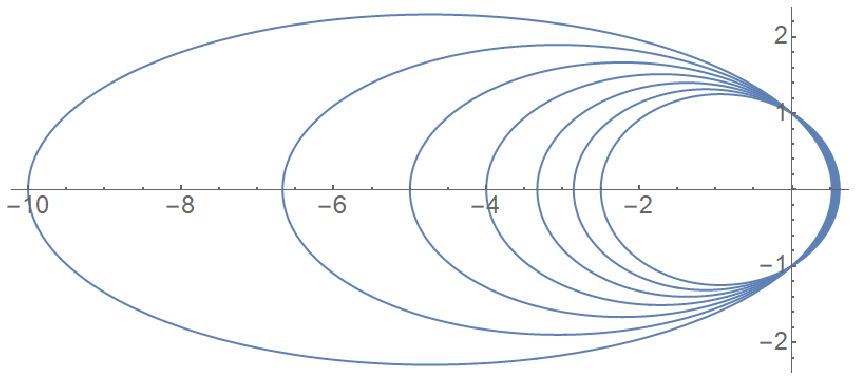
\includegraphics[width=.8\linewidth,height=6.5cm,keepaspectratio]{原图/kepler_ellipse}
\end{center}
\vfill
\noindent\begin{minipage}{\linewidth}
\small
本章从运动学描述出发，建立牛顿动力学、运动定理和守恒律，进而研究有心力轨道、有效势、稳定性、经典散射与变分方法。正文包括相关定理的完整推导、例题与练习解答。\par
\medskip
2026 年 10 月
\end{minipage}
\end{titlepage}
\pagenumbering{roman}
\begingroup
\small
\linespread{1.05}\selectfont
\makeatletter
\renewcommand{\@pnumwidth}{2.2em}
\renewcommand{\@tocrmarg}{3.2em}
\renewcommand*\l@section[2]{%
  \addvspace{4pt}%
  \@dottedtocline{1}{0em}{2.7em}{\bfseries #1}{\bfseries #2}}
\renewcommand*\l@subsection{\@dottedtocline{2}{1.5em}{3.2em}}
\makeatother
\tableofcontents
\endgroup
\clearpage
\section*{符号与基本约定}
\addcontentsline{toc}{section}{符号与基本约定}
讲义中的“静系”和“动系”是相对命名；静系是否为惯性系，需要另行判断。除非明确讨论变质量问题，质点质量 $m$ 为常数。求导时必须同时注意物理量的大小和基矢的方向。
\begin{center}
\small
\begin{tabularx}{\linewidth}{@{}lXlX@{}}
\toprule
符号&含义&符号&含义\\\midrule
$\vect r,\vect v,\vect a$&位矢、速度、加速度&$v=|\vect v|$&速率\\
$r,\theta$&平面极坐标&$s,\rho$&弧坐标、曲率半径\\
$\vect p=m\vect v$&动量&$\vect L=\vect r\times\vect p$&角动量\\
$T=\frac12mv^2$&动能&$U$&势能\\
$E=T+U$&机械能&$\ell=L/m$&比角动量\\
$\kappa>0$&平方反比力的强度&$\mu=GM$&引力参数\\
\bottomrule
\end{tabularx}
\end{center}
角动量记为 $L$，势能记为 $U$，有效势记为 $U_{\mathrm{eff}}$，速率记为 $v$。

正文中的 $U$、$L$、$b$ 分别表示势能、角动量和碰撞参数。图中若采用 $V$、$J$、$p$ 等其他记号，图题给出与正文的对应关系。正文先说明题设和坐标，再建立方程，图中的箭头和正方向应结合这些约定阅读。



\clearpage
\pagenumbering{arabic}

\section{运动描述与直角坐标}\label{sec:cartesian}

\subsection{质点、参考系与坐标系}
当物体的大小和形状对所研究的问题不产生显著影响时，可以把物体抽象为一个有质量、无几何尺寸的质点。这是针对具体问题建立的模型，同一物体在不同问题中可以有不同的处理方式。

\textbf{参考系}规定“相对于谁描述运动”；\textbf{坐标系}规定“用哪些数表示位置”。同一参考系中可以使用直角坐标、极坐标或自然坐标。改变坐标系不会改变该参考系中质点的运动，但各个分量的表达式会改变。

描述体系位置所需的独立坐标数称为\textbf{自由度}。空间自由质点有三个自由度；被限制在曲面上的质点通常有两个；被限制在给定曲线上的质点通常只有一个。约束使独立坐标减少，却可能引入未知的约束力。


\subsubsection*{理想化保留了什么}
研究地球绕太阳公转时，若只求轨道和周期，可以把地球视为质点；研究地球自转、潮汐或表面不同点的速度时，就需要考虑尺寸和姿态。质点模型保留质量、位置和相互作用，舍去姿态与形变。判断能否使用这一模型，应比较物体尺寸与问题中的距离尺度，并检查是否需要转动信息。

若空间质点满足一个独立几何约束 $f(x,y,z)=0$，局部可以用两个独立参数描述；再加一个独立约束，通常只剩一个参数。例如球面上的质点有两个自由度，固定圆环上的质点有一个。约束方程数只有在彼此独立时才能直接从三个坐标中扣除。

换参考系改变位置、速度等观测量；在同一参考系换坐标，只改变分量表达；改变物理模型，则改变要保留的运动信息和相互作用。


\subsection{位矢、运动方程与轨道}\label{topic:trajectory}
相对于固定原点 $O$，质点 $P$ 的位置矢量为 $\vect r=\overrightarrow{OP}$。若已知
\begin{equation}
\vect r=\vect r(t),
\end{equation}
就知道质点在各时刻的位置，这叫\textbf{运动方程}。运动方程包含时间信息。消去参数 $t$ 所得到的几何关系叫\textbf{轨道方程}，它只描述质点经过哪些位置。

例如 $x=A\cos\omega t,\ y=B\sin\omega t$，消去 $t$ 得
\[
\frac{x^2}{A^2}+\frac{y^2}{B^2}=1.
\]
同一条椭圆可以按不同的时间规律运动，因此仅有轨道方程还不足以确定速度和加速度。


\subsubsection*{轨道方程为什么不确定运动}
对半径为 $R$ 的圆，取 $x=R\cos\phi(t),\ y=R\sin\phi(t)$。无论 $\phi(t)=\omega t$ 还是 $\phi(t)=\alpha t^2/2$，消去时间都得到 $x^2+y^2=R^2$。前者角速度恒定，后者角加速度恒定；它们在同一条轨道上的速度与加速度完全不同。

还要区分运动学与动力学中的“方程”。$x=x(t)$ 是已经求出的运动规律；$m\ddot x=F(x,\dot x,t)$ 是决定运动规律的微分方程。后者一般需要初始条件才能求出前者。


\subsection{位移、路程、速度与加速度}\label{topic:displacement}
在 $t$ 到 $t+\Delta t$ 之间，位移是
\[
\Delta\vect r=\vect r(t+\Delta t)-\vect r(t).
\]
路程则是实际轨迹段的长度，是非负标量。一般有 $\Delta S\geq|\Delta\vect r|$；对光滑轨迹的无穷小段，$\dd S=|\dd\vect r|$。

速度和加速度的定义分别为
\begin{equation}
\vect v=\frac{\dd\vect r}{\dd t},\qquad
\vect a=\frac{\dd\vect v}{\dd t}=\frac{\dd^2\vect r}{\dd t^2}.
\end{equation}
速度沿轨迹切线、指向运动的一方。速率 $v=|\vect v|=\dd S/\dd t$ 描述运动快慢。加速度描述速度矢量的变化，既可以来自速率变化，也可以来自方向变化。
匀速圆周运动的速率不变，但速度方向一直变化，所以加速度不为零；在轨道上某一点速度为零，也不能据此认定该点加速度为零。


\subsubsection*{从有限变化到瞬时量}
在运动足够光滑时，位置的局部展开为
\[
\vect r(t+\Delta t)=\vect r(t)+\vect v(t)\Delta t
 +\frac12\vect a(t)(\Delta t)^2+O((\Delta t)^3).
\]
因此平均速度 $\Delta\vect r/\Delta t$ 在极限中趋于 $\vect v(t)$。速度箭头连接相邻时刻的位移信息，加速度箭头则连接相邻时刻的速度信息。沿轨迹前进一小段时，即使速度箭头长度相同，它们的差也可能不为零。

若 $\vect v\ne0$，用 $v^2=\vect v\cdot\vect v$ 求导，可得
\[
\dot v=\frac{\vect v\cdot\vect a}{v}.
\]
所以与速度平行的加速度分量决定速率变化；垂直分量改变方向。只有当 $\vect a$ 始终平行于同一个固定方向时，才可把矢量运动可靠地简化成该方向上的一维问题。在速度为零的瞬间，上式不能直接除以 $v$，应回到矢量定义或有向坐标。


\subsection{直角坐标系：固定基矢}\label{topic:cartesian}
若坐标轴固定在所选参考系上，则 $\vect e_x,\vect e_y,\vect e_z$ 不随时间变化。于是
\begin{align}
\vect r&=x\vect e_x+y\vect e_y+z\vect e_z,\\
\vect v&=\dot x\vect e_x+\dot y\vect e_y+\dot z\vect e_z,\\
\vect a&=\ddot x\vect e_x+\ddot y\vect e_y+\ddot z\vect e_z.
\end{align}
这里的点号始终表示对时间求导。直角坐标系的优点是基矢固定，求导直接；缺点是轨迹的几何特点有时不容易体现在方程中。

\example{椭圆规尺上某点的运动}\label{ex:ruler}
刚性直尺的两端 $A,B$ 分别被限制在水平、竖直光滑导轨上，导轨交点为 $O$。尺上固定点 $M$ 满足 $AM=a>0$、$BM=b>0$。取 $x$ 向右、$y$ 向上，考察 $A$ 在正半轴、$B$ 在正半轴的构形，杆与竖直方向夹角为 $0<\theta<\pi/2$。$B$ 端以恒定速率 $c>0$ 下降。求 $M$ 的轨道、速度和加速度，并说明端点构形处公式的适用性。
几何与变量约定见图\ref{fig:question-ex01}。

\QuestionFigure{ex01}{例1的研究对象、条件与变量}
\OriginalFigure{ellipse_rule}{椭圆规尺：两端分别沿坐标轴滑动，$AM=a$，$BM=b$。}
\solution \Step{模型与方向} 图\ref{fig:solution-ex01}给出解答所用的几何、方向或分解关系。图中的 $OA,OB$ 分别沿固定坐标轴；$M$ 是尺上的材料点，不能把它的速度直接等同于任一端点的速度。
\SolutionFigure{ex01}{解答中的几何、方向与计算关系}
\Step{建立方程与求解} 由几何关系，
\[
x=b\sin\theta,\quad y=a\cos\theta,\quad y_B=(a+b)\cos\theta.
\]
首先消去 $\theta$，得到椭圆轨道 $x^2/b^2+y^2/a^2=1$。由于 $\dot y_B=-c$，
\[
\dot\theta=\frac{c}{(a+b)\sin\theta}.
\]
因此
\begin{align*}
\dot x&=\frac{bc}{a+b}\cot\theta,&
\dot y&=-\frac{ac}{a+b},\\
\ddot x&=-\frac{bc^2}{(a+b)^2\sin^3\theta},&
\ddot y&=0.
\end{align*}
速率为 $v=\sqrt{\dot x^2+\dot y^2}$。$M$ 的加速度只有水平分量，尽管其轨道是曲线。公式适用于图示的这一段运动；$\sin\theta=0$ 附近不能维持有限杆端运动速度的同时保持上述理想匀速条件。



\Step{初始条件、结论与适用范围} 由图中 $y_B=L\cos\theta$，若初态为 $\theta_0$，则 $\cos\theta=\cos\theta_0-ct/L$，这补足了参数对时间的依赖。所写的分量式仅在同一几何分支、两导轨约束仍可维持的区间内使用。

\subsubsection*{椭圆规尺例题的中间计算}
令 $L=a+b$。由 $-L\sin\theta\,\dot\theta=-c$，先得到角速度；再对它求导：
\[
\ddot\theta=-\frac cL\frac{\cos\theta}{\sin^2\theta}\dot\theta
=-\frac{c^2\cos\theta}{L^2\sin^3\theta}.
\]
于是水平加速度为
\[
\ddot x=b(\cos\theta\,\ddot\theta-\sin\theta\,\dot\theta^2)
=-\frac{bc^2}{L^2}\frac{\cos^2\theta+\sin^2\theta}{\sin^3\theta},
\]
竖直分量则由 $y=(a/L)y_B$ 立即给出 $\ddot y=0$。这说明加速度的方向不能仅凭轨迹的凹向来猜测：曲线运动的总加速度包含切向与法向两部分。

也可不用角度直接写 $x=b\sqrt{1-(y_B/L)^2}$，再代入 $y_B(t)=y_{B0}-ct$ 求导。两种解法分别突出几何参数和输入运动规律。初始杆近于竖直时，给 $B$ 端强行规定有限下降速率，会要求 $A$ 端有很大的水平速率；公式的发散反映这个理想运动条件的局限。

\section{曲线运动的坐标方法}\label{sec:curvilinear}

\subsection{平面极坐标系：基矢也要求导}\label{topic:polar}
对于平面运动，取 $r\geq0$，$\theta$ 为从极轴沿规定正方向量取的角度。径向单位矢量 $\er$ 沿位矢方向，横向单位矢量 $\et$ 指向 $\theta$ 增大的方向。
\OriginalFigure{polar_basis}{平面极坐标基矢。图中的 $\bm i,\bm j$ 分别对应正文的 $\er,\et$。}
在固定直角基矢中写出
\[
\er=\cos\theta\vect e_x+\sin\theta\vect e_y,\qquad
\et=-\sin\theta\vect e_x+\cos\theta\vect e_y.
\]
逐项求导得
\begin{equation}\label{eq:basis}
\dot{\er}=\dot\theta\et,\qquad
\dot{\et}=-\dot\theta\er.
\end{equation}
由 $\vect r=r\er$，
\begin{equation}\label{eq:polarv}
\vect v=\dot r\er+r\dot\theta\et.
\end{equation}
再次求导，保留每一项：
\begin{align*}
\vect a
&=\ddot r\er+\dot r\dot{\er}
 +(\dot r\dot\theta+r\ddot\theta)\et+r\dot\theta\dot{\et}\\
&=(\ddot r-r\dot\theta^2)\er
 +(r\ddot\theta+2\dot r\dot\theta)\et.
\end{align*}
\textbf{极坐标分量}\quad
\[
v_r=\dot r,\quad v_\theta=r\dot\theta,\qquad
a_r=\ddot r-r\dot\theta^2,\quad
a_\theta=r\ddot\theta+2\dot r\dot\theta.
\]
径向分量不等于 $\ddot r$；横向分量不等于 $r\ddot\theta$。变化的基矢贡献了额外项。
若 $r=R$ 为常数，就退化为圆周运动：$a_r=-R\dot\theta^2=-v^2/R$，$a_\theta=R\ddot\theta$。若 $\theta$ 为常数，则是沿固定射线的直线运动。


\subsubsection*{怎样理解两项横向贡献}
$\dot r\er$ 的方向随极角改变，它的导数贡献 $\dot r\dot\theta\et$；$r\dot\theta\et$ 的大小又因半径改变，其导数再贡献同样的一项。因此 $2\dot r\dot\theta$ 并非一个重复计算，而是两个不同来源的总和。这里的极坐标建立在惯性参考系中，出现这些项并不等于参考系本身在转动。

从直角坐标检查径向分量也很有帮助。因为 $r^2=x^2+y^2$，
\[
\dot r=\frac{x\dot x+y\dot y}{r}=\vect v\cdot\er,
\qquad
v^2=\dot r^2+r^2\dot\theta^2.
\]
$\dot r$ 只测量远离或接近极点的快慢。绕极点转动时即使 $\dot r=0$，质点仍可具有非零速度。


\example{指数展开的螺旋轨道}
质点在固定平面内运动，以固定点 $O$ 为极点，极角从 $+x$ 轴逆时针量起。已知 $r(t)=r_0e^{ct}$、$\theta(t)=bt$，$r_0>0$，$b,c$ 为常数。求矢量速度、矢量加速度、两者的大小及轨道方程；再求切向、法向加速度和曲率半径，分别讨论 $b=0$ 与 $c=0$ 的情形。
几何与变量约定见图\ref{fig:question-ex02}。

\QuestionFigure{ex02}{例2的研究对象、条件与变量}

\solution \Step{模型与方向} 图\ref{fig:solution-ex02}给出解答所用的几何、方向或分解关系。图中的径向 $\er$ 和横向 $\et$ 随 $P$ 转动，合速度沿螺旋线切线。因而对位矢求导时必须同时求基矢的导数。
\SolutionFigure{ex02}{解答中的几何、方向与计算关系}
\Step{建立方程与求解} 有 $\dot r=cr,\ \ddot r=c^2r,\ \dot\theta=b,\ \ddot\theta=0$。代入极坐标公式得
\[
\vect v=r(c\er+b\et),\qquad
\vect a=r[(c^2-b^2)\er+2bc\et].
\]
于是
\[
v=r\sqrt{b^2+c^2},\qquad
|\vect a|=r(b^2+c^2).
\]
当 $b\ne0$ 时，消去时间得 $r=r_0\mathrm e^{(c/b)\theta}$，这是一条对数螺旋线。当 $c=0$ 时结果回到匀速圆周运动。


\subsubsection*{螺旋运动的自然坐标分量}
加速度的模来自
\[
(c^2-b^2)^2+(2bc)^2=(b^2+c^2)^2.
\]
若 $b\ne0$，则 $\dot v=cv$，所以切向加速度为 $a_t=cr\sqrt{b^2+c^2}$，其符号随 $c$ 改变。利用 $a_n^2=|\vect a|^2-a_t^2$ 得
\[
a_n=r|b|\sqrt{b^2+c^2},\qquad
\rho=\frac{v^2}{a_n}=\frac{r\sqrt{b^2+c^2}}{|b|}.
\]
速度与径向之间的夹角不随时间变化，因为 $v_\theta/v_r=b/c$ 为常数。$b=0$ 时是沿射线的运动，曲率为零，需要单独取直线极限。

\example{小车匀速，绳上的点是否匀速？}\label{ex:rope}
一根轻且不可伸长的绳，一端系在水平轨道上的小车 $A$，经过离轨道高度为 $h>0$ 的固定理想滑轮 $B$，另一部分绕在鼓轮 $C$ 上。绳在直线段 $BC$ 上始终绷紧、沿固定方向运动。小车以恒定速率 $v>0$ 远离 $B$ 的正下方 $O$。忽略滑轮尺寸，令 $OA=x$。求直绳段上材料点 $P$ 的速度和加速度，并求斜绳与竖直方向成 $45^\circ$ 时的结果。
几何与变量约定见图\ref{fig:question-ex03}。

\QuestionFigure{ex03}{例3的研究对象、条件与变量}
\OriginalFigure{pulley_cart}{小车与不可伸长绳。$\theta$ 从竖直方向量起，绳上点 $P$ 朝滑轮 $B$ 运动。}
\solution \Step{模型与方向} 图\ref{fig:solution-ex03}给出解答所用的几何、方向或分解关系。图中的 $AB$ 长度随 $x$ 改变；绳不可伸长使这段的长度变化由 $BC$ 上绳点的移动补偿。$P$ 所在绳段是直线，其加速度沿该绳段。
\SolutionFigure{ex03}{解答中的几何、方向与计算关系}
\Step{建立方程与求解} 设车到滑轮正下方的水平距离为 $x$，则 $\dot x=v$，斜绳长 $l=\sqrt{x^2+h^2}$。鼓轮向绳段 $AB$ 放绳，$P$ 沿 $BC$ 朝滑轮 $B$ 运动，其速率为
\[
w=\dot l=\frac{vx}{\sqrt{x^2+h^2}}.
\]
沿 $C$ 指向 $B$ 的绳方向为正，
\[
\dot w=\frac{v^2h^2}{(x^2+h^2)^{3/2}}.
\]
图中 $\theta$ 为斜绳与竖直线的夹角，故 $x=h\tan\theta$。当 $\theta=45^\circ$ 时，
\[
w=\frac{v}{\sqrt2},\qquad
\dot w=\frac{v^2}{2\sqrt2\,h}.
\]
绳点向滑轮运动且正在加速，加速度同样指向滑轮。不可伸长条件约束的是绳长关系，不能把小车的水平速度直接当成绳的速度。



\subsubsection*{绳速的另外两种推导方法}
\textbf{极坐标法。} 取固定滑轮 $B$ 为极点，$A$ 的径向坐标为 $l$，角度 $\theta$ 从竖直向下量起。车速在两条极坐标基矢的投影为 $v_r=v\sin\theta$、$v_\theta=v\cos\theta$，因此 $\dot l=v\sin\theta$、$l\dot\theta=v\cos\theta$。车的绝对加速度为零，径向分量式 $0=\ddot l-l\dot\theta^2$ 给出
\[
a_P=\ddot l=\frac{v^2\cos^2\theta}{l}=\frac{v^2\cos^3\theta}{h}.
\]
这里 $l\dot\theta^2$ 是车在极坐标分解中的向心项，$\ddot l$ 是绳速变化率；二者数值相等来自车的径向加速度恰好为零，不能把绳点在直线段上的加速度说成其自身的圆周向心加速度。

\textbf{有限变化取极限。} 令 $\Delta t$ 内车水平位移为 $v\Delta t$，则斜绳长增量为
\[
\Delta l=\sqrt{h^2+(x+v\Delta t)^2}-\sqrt{h^2+x^2}.
\]
对 $\Delta t$ 展开，
\[
\Delta l=\frac{vx}{l}\Delta t+\frac{v^2h^2}{2l^3}(\Delta t)^2+O((\Delta t)^3).
\]
一次项给出绳速 $vx/l=v\sin\theta$，二次项的两倍给出加速度 $v^2h^2/l^3$。这说明微元法、泰勒展开与直接求导来自同一极限过程。

\subsubsection*{绳长约束的求导与极限}
斜绳长增加的速率可以直接由
\[
\dot l=\frac{1}{2}(x^2+h^2)^{-1/2}(2x\dot x)
\]
得到。它等于小车速度在斜绳方向上的投影 $v\sin\theta$。即使小车匀速，投影角也在变化，故绳点加速。再求导时必须使用 $\dot x=v$：
\[
\dot w=v^2\left[\frac1{\sqrt{x^2+h^2}}
 -\frac{x^2}{(x^2+h^2)^{3/2}}\right].
\]
当 $x=0$ 时，$w=0$ 但 $\dot w=v^2/h$；当 $x\gg h$ 时，$w\to v$ 而 $\dot w\to0$。这两个极限同时核验了速度和加速度的几何意义。

\example{心形线运动的速度与加速度}\label{ex:cardioid}
在固定平面极坐标中，质点满足 $r=a(1-\cos\omega t)$、$\theta=\omega t$，$a,\omega>0$，极角从 $+x$ 轴逆时针量起。求一般时刻的速度与加速度；在 $t=\pi/(2\omega)$ 时，把结果同时写成极坐标分量和固定直角坐标分量，并求速率与加速度大小。
几何与变量约定见图\ref{fig:question-ex04}。

\QuestionFigure{ex04}{例4的研究对象、条件与变量}

\solution \Step{模型与方向} 结合题图\ref{fig:question-ex04}，解答图\ref{fig:solution-ex04}展示指定位置 $P$ 处的速度与加速度首尾分解；$\er$ 向上、$\et$ 向左，因此径向负分量在固定坐标中向下，两幅矢量图分别对应下面的速度式与加速度式。
\SolutionFigure{ex04}{解答中的几何、方向与计算关系}
\Step{建立方程与求解} 先求坐标导数，再代入极坐标公式：
\[
\dot r=a\omega\sin\theta,\quad\ddot r=a\omega^2\cos\theta,
\qquad\dot\theta=\omega,\quad\ddot\theta=0.
\]
因此任意时刻
\begin{align*}
\vect v&=a\omega[\sin\theta\,\er+(1-\cos\theta)\et],\\
\vect a&=a\omega^2[(2\cos\theta-1)\er+2\sin\theta\,\et].
\end{align*}
在指定时刻 $\theta=\pi/2$，所以
\[
\vect v=a\omega(\er+\et),\quad
\vect a=a\omega^2(-\er+2\et),\quad v=\sqrt2a\omega,\quad |\vect a|=\sqrt5a\omega^2.
\]
这里的 $\er,\et$ 是该时刻的局部基矢，不能当作固定的 $x,y$ 基矢：此时 $\er=\vect e_y$、$\et=-\vect e_x$，故 $\vect v=a\omega(-\vect e_x+\vect e_y)$、$\vect a=a\omega^2(-2\vect e_x-\vect e_y)$。
\OriginalFigure{cardioid_original}{极坐标运动 $r=e(1-\cos\omega t)$、$\varphi=\omega t$ 的心形线轨迹；其中 $e=a$、$\varphi=\theta$。}


\subsubsection*{极坐标运动的三个应用}\label{ex:polarpractice}

\Case{应用一：径向匀速且极角匀速增加}
\textbf{题目。} 质点在固定平面内满足 $r=at,\theta=bt$，$a>0$，$b$ 为常数，$t\ge0$。极角从 $+x$ 轴逆时针量起。求速度、加速度及其大小，消去时间写出轨道；说明 $b=0$ 与初始极点处的含义。
模型与变量见图\ref{fig:question-pl01}。
\QuestionFigure{pl01}{径向与横向基矢及轨道分支示意；图取 $b>0$}
\solution \Step{先确定随动基矢} 图\ref{fig:solution-pl01}中 $\er$ 沿 $OP$ 向外，$\et$ 沿极角增加方向。即使 $\dot r$ 恒定，这两个方向仍随时间变化。
\SolutionFigure{pl01}{极坐标基矢的转动与速度合成}
\Step{逐次求导} 由 $\dot r=a,\ddot r=0,\dot\theta=b,\ddot\theta=0$，代入完整极坐标式得
\[
\vect v=a\er+abt\et,\qquad
\vect a=-ab^2t\er+2ab\et.
\]
其中径向加速度来自横向速度方向的改变，横向项的两份 $ab$ 分别来自 $\dot r\er$ 的方向转动和 $r\dot\theta\et$ 的系数改变。两基矢正交，故
\[
v=a\sqrt{1+b^2t^2},\qquad |\vect a|=|ab|\sqrt{4+b^2t^2}.
\]
\Step{轨道与初始极限} 若 $b\ne0$，有 $r=(a/b)\theta$，取与 $t\ge0$ 相容的连续角度分支；若 $b=0$，为沿 $+x$ 的匀速直线运动。极点处由 $x=at\cos bt,y=at\sin bt$ 求固定坐标极限，得到 $\vect v(0)=a\vect e_x$、$\vect a(0)=2ab\vect e_y$，物理量没有发散。

\Case{应用二：圆环上的均匀增速运动}
\textbf{题目。} 小环沿半径 $R>0$ 的固定圆环运动，初始位于角度零点，随后沿逆时针运动，速率为 $v=at$，$a>0$、$t\ge0$。求弧长与转角、速度和加速度，给出总加速度相对切线的方向及初态极限。
模型与变量见图\ref{fig:question-pl02}。
\QuestionFigure{pl02}{圆周运动的局部切向与主法向}
\solution \Step{位置规律与局部方向} 图\ref{fig:solution-pl02}以 $\vt$ 表示前进方向，$\vn=-\er$ 指向圆心；图上局部方向可随圆周位置整体转动。
\SolutionFigure{pl02}{切向增速与法向转弯两种加速度}
从 $s(0)=0$ 积分得 $s=at^2/2$，所以 $\theta=at^2/(2R)$。速度为 $\vect v=at\vt$。
\Step{分别计算两分量} 因曲率半径为 $R$，
\[
a_t=\dot v=a,\qquad a_n=\frac{v^2}{R}=\frac{a^2t^2}{R},\qquad
\vect a=a\vt+\frac{a^2t^2}{R}\vn.
\]
于是 $|\vect a|=a\sqrt{1+a^2t^4/R^2}$，相对前进切线的内偏角满足 $\tan\beta=at^2/R$。初态虽 $v=0$，仍有切向加速度 $a$，只是法向分量为零。轨道为圆并不意味着匀速，不能遗漏切向项。

\Case{应用三：由一般极坐标轨道恢复运动分量}
\textbf{题目。} 质点沿给定光滑曲线 $r=f(\theta)>0$ 运动，$f$ 二次可微；其时间规律为给定的 $\theta=\theta(t)$。求速度与加速度的普遍分量式，指出式中各导数的自变量，并说明仅给轨道能否确定运动。
模型与变量见图\ref{fig:question-pl03}。
\QuestionFigure{pl03}{一般极坐标曲线的径向与横向；曲线形状为示意}
\solution \Step{先把几何函数转换为时间导数} 在图\ref{fig:solution-pl03}中，$OP=f(\theta)$，而基矢随 $\theta(t)$ 转动。记 $f'=\dd f/\dd\theta$、$f''=\dd^2 f/\dd\theta^2$，链式法则给出
\[
\dot r=f'\dot\theta,\qquad \ddot r=f''\dot\theta^2+f'\ddot\theta.
\]
\SolutionFigure{pl03}{沿给定曲线的基矢转动与局部分解}
\Step{代入完整运动学公式} 分别整理径向与横向系数，得到
\begin{align*}
\vect v&=\dot\theta(f'\er+f\et),\\
\vect a&=[(f''-f)\dot\theta^2+f'\ddot\theta]\er
       +[2f'\dot\theta^2+f\ddot\theta]\et.
\end{align*}
因而 $v=|\dot\theta|\sqrt{f'^2+f^2}$。同一曲线可用不同的 $\theta(t)$ 通过，因此轨道几何不能单独确定速度和加速度；还须给时间规律或能确定它的动力学初值问题。

\subsection{自然坐标系：把速率变化与转弯分开}\label{topic:natural}
在给定轨迹上选择起点和正方向，用有向弧坐标 $s$ 表示位置。定义切向单位矢量 $\vt=\dd\vect r/\dd s$，主法向单位矢量 $\vn$ 指向曲率中心。对于光滑曲线，
\[
\frac{\dd\vt}{\dd s}=\frac{1}{\rho}\vn.
\]
因此
\begin{equation}\label{eq:natural}
\vect v=\dot s\vt,\qquad
\vect a=\ddot s\vt+\frac{\dot s^{\,2}}{\rho}\vn.
\end{equation}
若把切向正方向取为当前运动方向，可写 $\vect a=\dot v\vt+(v^2/\rho)\vn$。这一写法在质点掉头时须重新处理方向；采用有向弧坐标的式\eqref{eq:natural} 更统一。
\OriginalFigure{natural_frame}{相邻位置的切线与切向基矢之差。图中的 $\bm i$ 对应正文的 $\vt$，下部展示基矢相减。}
切向加速度改变速率，法向加速度改变方向。空间曲线还有从法向基矢 $\vect e_b=\vt\times\vn$，但速度和加速度均处于切线与主法线张成的平面内，因此加速度的从法向分量为零。


\subsubsection*{自然坐标公式的几何推导}
相邻两点的切线夹角为 $\Delta\psi$。把两个单位切向矢量移到同一起点，它们的差在极限中垂直切线，模长为 $\Delta\psi$。密切圆给出 $\Delta\psi/\Delta s\to1/\rho$，从而得到 $\dd\vt/\dd s=\vn/\rho$。

对 $\vect v=\dot s\vt$ 使用乘积法则，
\[
\frac{\dd\vect v}{\dd t}=\ddot s\vt
 +\dot s\frac{\dd\vt}{\dd s}\dot s,
\]
就得到式\eqref{eq:natural}。法向加速度中是 $\dot s^{\,2}$，所以无论质点沿曲线哪一方向运动，法向分量都指向同一个局部曲率中心。


\subsubsection*{曲率半径的计算}\label{topic:curvature}
若平面轨道为 $y=y(x)$，
\begin{equation}
\rho=\frac{[1+(y')^2]^{3/2}}{|y''|}.
\end{equation}
若曲线用任意参数 $u$ 表示为 $\vect r(u)$，且 $\vect r'(u)\ne0$，则
\begin{equation}
\rho=\frac{|\vect r'(u)|^3}{|\vect r'(u)\times\vect r''(u)|}.
\end{equation}
此处撇号表示对 $u$ 求导，不是对时间求导。直线的曲率为零，可理解为 $\rho\to\infty$。


对 $y(x)$，令切线方向角为 $\psi$，则 $\tan\psi=y'$，而 $\dd s=\sqrt{1+(y')^2}\,\dd x$。因此
\[
\left|\frac{\dd\psi}{\dd s}\right|
=\frac{|y''|}{[1+(y')^2]^{3/2}}=\frac1\rho.
\]
对任意参数曲线，$\vect r''$ 的切向部分只改变参数前进的快慢；叉积 $\vect r'\times\vect r''$ 消去了这一部分，留下弯曲信息。这也是曲率公式不依赖参数选择的原因。


\example{已知单摆的角度变化，求速度和加速度}\label{ex:pendkin}
长为 $l>0$ 的不可伸长轻杆绕固定点 $O$ 在竖直平面内运动，端点为 $P$。摆角 $\varphi$ 从竖直向下逆时针量起，给定运动规律 $\varphi(t)=\varphi_0\sin\omega t$，$\omega>0$。把它作为已知运动学规律，不预设它是大振幅单摆的动力学精确解。求 $P$ 的速度、切向和法向加速度，说明转向时速度为零是否意味着加速度为零。
几何与变量约定见图\ref{fig:question-ex05}。

\QuestionFigure{ex05}{例5的研究对象、条件与变量}
\OriginalFigure{pendulum}{单摆的摆角 $\varphi$ 和有向弧坐标 $s=l\varphi$。}
\solution \Step{模型与方向} 图\ref{fig:solution-ex05}给出解答所用的几何、方向或分解关系。图中的 $OP=l$ 保持不变，$\vect e_\varphi$ 指向摆角增加方向，主法向指向悬点。速度随 $\dot\varphi$ 取正负，法向加速度则始终向内。
\SolutionFigure{ex05}{解答中的几何、方向与计算关系}
\Step{建立方程与求解} 取 $s=l\varphi$，曲率半径为 $l$。于是
\begin{align*}
\vect v&=l\varphi_0\omega\cos\omega t\,\vt,\\
\vect a&=-l\varphi_0\omega^2\sin\omega t\,\vt
 +l\varphi_0^2\omega^2\cos^2\omega t\,\vn.
\end{align*}
在最低点，切向加速度为零、法向加速度不为零；在摆动端点，速度为零、切向加速度一般不为零。
\Step{初始条件、结论与适用范围} 把给定摆角求导得 $\dot\varphi=\varphi_0\omega\cos\omega t$、$\ddot\varphi=-\varphi_0\omega^2\sin\omega t$。于是 $\vect v=l\dot\varphi\vect e_\varphi$、$\vect a=l\ddot\varphi\vect e_\varphi-l\dot\varphi^2\vect e_r$。在摆角极值处 $\dot\varphi=0$，但一般 $\ddot\varphi\ne0$，因此只有法向分量消失。



\example{沿抛物线匀速运动的最低点加速度}\label{ex:parabolak}
质点在固定竖直平面内沿抛物线 $y=kx^2$ 运动，$k>0$，$x$ 水平向右、$y$ 竖直向上。自顶点起向右取弧长正向，给定 $s=ct$，$c>0$。求质点通过顶点时的加速度大小和方向；进一步求一般横坐标 $x$ 处的曲率半径与加速度。
几何与变量约定见图\ref{fig:question-ex06}。

\QuestionFigure{ex06}{例6的研究对象、条件与变量}

\solution \Step{模型与方向} 图\ref{fig:solution-ex06}给出解答所用的几何、方向或分解关系。图中的切线沿轨道前进方向，主法线指向抛物线凹侧。恒速消去切向分量，剩余加速度由图示曲率半径决定。
\SolutionFigure{ex06}{解答中的几何、方向与计算关系}
\Step{建立方程与求解} 速率为常数 $c$，故切向加速度为零。顶点处 $y'=0,\ y''=2k$，所以 $\rho=1/(2k)$。主法线向上，得到
\[
\vect a=2kc^2\vect e_y.
\]



\Step{推广到一般位置}
对 $y=kx^2$，曲率半径为 $\rho=(1+4k^2x^2)^{3/2}/(2k)$，主法向单位矢量为
\[
\vn=\frac{-2kx\vect e_x+\vect e_y}{\sqrt{1+4k^2x^2}}.
\]
当速率恒为 $c$ 时，
\[
\vect a=\frac{2kc^2}{(1+4k^2x^2)^2}
 (-2kx\vect e_x+\vect e_y).
\]
虽然速率不变，加速度的大小却随位置变化；顶点的弯曲最强，所以加速度最大。轨道的几何形状决定法向方向与曲率，运动的时间规律决定切向加速度和速率。

\example{速率线性增加的空间螺旋线运动}\label{ex:helixkin}
空间曲线用参数 $u$ 表示为 $\vect r(u)=(R\cos u,R\sin u,bu)$，其中 $R>0$，$b$ 为常数。质点从 $u=0$ 出发，沿 $u$ 增大方向运动，速率给定为 $v=at$，$a>0,t\ge0$。求 $u(t)$、曲率半径以及切向、法向和总加速度，说明两个分量分别对应怎样的运动变化。
几何与变量约定见图\ref{fig:question-ex07}。

\QuestionFigure{ex07}{例7的研究对象、条件与变量}

\solution \Step{模型与方向} 图\ref{fig:solution-ex07}给出解答所用的几何、方向或分解关系。螺旋线的主法线水平指向圆柱轴线，切线还含轴向分量。图中的 $\vt,\vn$ 应先用轨道几何确定，再分别乘速率变化率和 $v^2/\rho$。
\SolutionFigure{ex07}{解答中的几何、方向与计算关系}
\Step{建立方程与求解} $|\vect r_u|=\sqrt{R^2+b^2}$，$\vect r_{uu}=(-R\cos u,-R\sin u,0)$，且 $\vect r_u\cdot\vect r_{uu}=0$，因此
\[
\rho=\frac{R^2+b^2}{R},\qquad
\vect a=a\vt+\frac{a^2t^2R}{R^2+b^2}\vn.
\]
其中 $\vt=(-R\sin u,R\cos u,b)/\sqrt{R^2+b^2}$、$\vn=(-\cos u,-\sin u,0)$。若取 $u$ 增大为运动方向，则 $\dot u=at/\sqrt{R^2+b^2}$，积分得 $u=u_0+at^2/[2\sqrt{R^2+b^2}]$，代回基矢即可把加速度完整写成时间函数。此题指定运动学速率，不能用仅有重力的螺旋线动力学方程代替。
\OriginalFigure{helix_original}{圆柱螺旋线的空间形状。图中的半径 $a$ 对应正文的 $R$。}


\Step{初始条件、结论与适用范围} 弧长元为 $\dd s=\sqrt{R^2+b^2}\,\dd u$，故 $\dot u=at/\sqrt{R^2+b^2}$。由 $u(0)=0$ 得 $u=at^2/(2\sqrt{R^2+b^2})$。这一参数关系才把空间曲线变成确定的时间运动。

\subsubsection*{空间曲线的完整 Frenet--Serret 关系}\label{topic:frenet}

对光滑正则曲线，在曲率 $\kappa=1/\rho>0$ 的点定义 $\vect e_b=\vt\times\vn$。三条基矢均随弧长变化：
\begin{equation}\label{eq:frenet}
\frac{\dd\vt}{\dd s}=\kappa\vn,\qquad
\frac{\dd\vn}{\dd s}=-\kappa\vt+\tau\vect e_b,\qquad
\frac{\dd\vect e_b}{\dd s}=-\tau\vn.
\end{equation}
第一式描述切线转弯，第三式描述密切平面转动；$\tau$ 称为挠率，其符号取决于空间曲线的定向约定。第二式中的切向系数来自 $\dd(\vt\cdot\vn)/\dd s=0$；副法向系数由第三式和正交性确定。对一般参数 $u$，
\[
\kappa=\frac{|\vect r'\times\vect r''|}{|\vect r'|^3},\qquad
\tau=\frac{(\vect r'\times\vect r'')\cdot\vect r'''}{|\vect r'\times\vect r''|^2}.
\]
圆柱螺旋线 $\vect r(u)=(R\cos u,R\sin u,bu)$ 有 $\kappa=R/(R^2+b^2)$、$\tau=b/(R^2+b^2)$。当 $b=0$ 时变成平面圆，挠率为零。在曲率为零的点，上述主法线和挠率定义需另行延拓，不能直接除以零。

虽然三条基矢都在变化，质点加速度仍为 $\dot v\vt+v^2\kappa\vn$，没有副法向分量，因为速度只含 $v\vt$；挠率首先出现在加速度的时间导数中。这解释了三维轨迹的自然坐标动力学为什么仍有 $a_b=0$。


\subsubsection*{自然坐标中的运动分类}\label{ex:naturalthinking}
\Case{应用一：法向加速度为零}
\textbf{题目。} 一段光滑平面运动在整个区间内满足 $v(t)>0$、$a_n(t)=0$。判断轨道形状，说明切向加速度能否非零，并给出一个具体运动作为例子。
模型与变量见图\ref{fig:question-na01}。
\QuestionFigure{na01}{直线变速运动与恒速圆周运动的区别}
\solution \Step{用非静止条件确定曲率} 结合题图\ref{fig:question-na01}，解答图\ref{fig:solution-na01}展示直线上的不等长速度矢量与圆周上的切向速度、向心加速度；左侧只改变速度大小，右侧只改变速度方向，所以分别对应切向项与法向项，不能由一个分量为零推出整个加速度为零。
\SolutionFigure{na01}{直线上的切向加速与圆周上的法向加速}
\Step{构造满足条件的运动} 取 $x=v_0t+a_0t^2/2$，$v_0,a_0>0,t\ge0$，则 $v_x=v_0+a_0t>0$，$a_t=a_0$，$a_n=0$。因此直线轨道并不限制速率恒定。若只知一个静止瞬间 $v=0$，不能由此判定邻近轨道的曲率。

\Case{应用二：切向加速度为零}
\textbf{题目。} 一段运动始终有 $v>0$、$a_t=0$。能否断定轨道为圆？请用固定抛物线 $y=kx^2$、$k>0$ 上的恒速运动给出完整反例，并求其法向加速度。
模型与变量见图\ref{fig:question-na03}。
\QuestionFigure{na03}{恒速通过抛物线；主法线随位置改变}
\solution \Step{速率条件不决定几何曲率} 图\ref{fig:solution-na03}中 $\vt$ 沿抛物线前进方向。$a_t=\dot v=0$ 只给出 $v=v_0$；对给定抛物线，曲率为
\[
\kappa=\frac{2k}{(1+4k^2x^2)^{3/2}},\qquad
a_n=\frac{2kv_0^2}{(1+4k^2x^2)^{3/2}}.
\]
\SolutionFigure{na03}{恒速运动仍有沿凹侧的法向加速度}
\Step{判断结论} 该曲率随 $x$ 改变，所以轨道并非圆，但始终满足 $a_t=0$。图中的加速度沿主法线；“只有法向分量”可以出现在任意光滑曲线的恒速运动中。

\Case{应用三：同时具有切向与法向分量}
\textbf{题目。} 小环在半径 $R>0$ 的固定圆环上以速率 $v=v_0+ct$ 运动，$v_0,c>0,t\ge0$。求两个加速度分量及合加速度方向，说明与恒速圆周运动有何区别。
模型与变量见图\ref{fig:question-na02}。
\QuestionFigure{na02}{圆环上的局部切向与主法向}
\solution \Step{分别处理增速与转弯} 图\ref{fig:solution-na02}中内法线始终指向圆心，故
\[
a_t=c,\qquad a_n=\frac{(v_0+ct)^2}{R},\qquad
\vect a=c\vt+\frac{(v_0+ct)^2}{R}\vn.
\]
\SolutionFigure{na02}{变速圆周运动中的两个正交分量}
\Step{合成方向} 两分量都非零，$|\vect a|=\sqrt{c^2+(v_0+ct)^4/R^2}$，相对前进切线向内偏角满足 $\tan\beta=(v_0+ct)^2/(Rc)$。令 $c\to0$，才恢复纯法向的恒速圆周运动。

\example{竖直速度分量恒定时的加速度}\label{ex:constantvy}
质点在固定 $xy$ 平面内作光滑曲线运动，竖直速度分量恒为 $v_y=c\ne0$。在某个速率 $v>0$、曲率半径为 $\rho$ 的位置，求总加速度大小与 $v,c,\rho$ 的关系。证明结论，并讨论直线段和 $c=0$ 时为什么需要另行处理。
几何与变量约定见图\ref{fig:question-ex08}。

\QuestionFigure{ex08}{例8的研究对象、条件与变量}

\solution \Step{模型与方向} 图\ref{fig:solution-ex08}给出解答所用的几何、方向或分解关系。图中的等时位移具有相同竖直分量，因此 $a_y=0$。加速度箭头水平，但并不一般沿轨道主法线，须用速度与加速度的叉积求曲率。
\SolutionFigure{ex08}{解答中的几何、方向与计算关系}
\Step{建立方程与求解} 由 $a_y=0$，加速度沿 $x$ 轴。利用平面曲率的矢量表达式，
\[
\frac1\rho=\frac{|v_xa_y-v_ya_x|}{v^3}=\frac{|c|\,|a_x|}{v^3}.
\]
所以 $a=|a_x|=v^3/(|c|\rho)$。若 $c>0$，可写成 $v^3/(c\rho)$；一般情形需取绝对值。若 $c=0$，运动沿水平直线，曲率为零，不能使用这个商式。
\Step{初始条件、结论与适用范围} 若轨道在某区间为直线且 $c\ne0$，则直线斜率固定；由竖直速度固定可推出总速度固定，所以该区间 $a=0$，与 $\rho\to\infty$ 的极限相容。对于曲率非零的点，先由叉积确定加速度大小，再由给定轨道的弯曲方向确定 $a_x$ 的符号；仅有 $v,c,\rho$ 不能区分向左弯和向右弯。



\subsection{空间运动：柱坐标与球坐标}\label{topic:column}

柱坐标记为 $(\varrho,\phi,z)$，与平面极坐标相比增加独立的竖直方向：
\begin{align*}
\vect v&=\dot\varrho\vect e_\varrho+\varrho\dot\phi\vect e_\phi+\dot z\vect e_z,\\
\vect a&=(\ddot\varrho-\varrho\dot\phi^2)\vect e_\varrho
 +(\varrho\ddot\phi+2\dot\varrho\dot\phi)\vect e_\phi+\ddot z\vect e_z.
\end{align*}
球坐标记为 $(r,\vartheta,\phi)$，\textbf{$\vartheta$ 从 $z$ 正轴量起}，$\phi$ 为方位角：
\[
x=r\sin\vartheta\cos\phi,\quad
y=r\sin\vartheta\sin\phi,\quad z=r\cos\vartheta.
\]
速度为
\[
\vect v=\dot r\er+r\dot\vartheta\vect e_\vartheta
 +r\sin\vartheta\dot\phi\vect e_\phi.
\]
加速度的三个分量为
\begin{align*}
a_r&=\ddot r-r\dot\vartheta^2-r\sin^2\vartheta\dot\phi^2,\\
a_\vartheta&=r\ddot\vartheta+2\dot r\dot\vartheta
 -r\sin\vartheta\cos\vartheta\dot\phi^2,\\
a_\phi&=r\sin\vartheta\ddot\phi
 +2\dot r\sin\vartheta\dot\phi
 +2r\cos\vartheta\dot\vartheta\dot\phi.
\end{align*}
由势能求力时，梯度也要带上尺度因子：
\begin{align*}
\nabla U&=\vect e_\varrho\partial_\varrho U
 +\vect e_\phi\frac1\varrho\partial_\phi U+\vect e_z\partial_zU
 &&\text{（柱坐标）},\\
\nabla U&=\er\partial_rU+\vect e_\vartheta\frac1r\partial_\vartheta U
 +\vect e_\phi\frac1{r\sin\vartheta}\partial_\phi U
 &&\text{（球坐标）}.
\end{align*}


\subsubsection*{尺度因子从哪里来}
球坐标中微小位移沿三个正交方向分解为
\[
\dd\vect r=\er\dd r+r\vect e_\vartheta\dd\vartheta
 +r\sin\vartheta\vect e_\phi\dd\phi.
\]
改变极角 $\vartheta$ 对应半径为 $r$ 的圆弧；改变方位角 $\phi$ 对应半径为 $r\sin\vartheta$ 的纬线圆弧。因此速度分量和梯度公式中的 $r,r\sin\vartheta$ 都来自几何长度，而非可任意省略的系数。

若 $\vartheta=\pi/2$ 且 $\dot\vartheta=0$，球坐标运动退化为赤道平面内的极坐标运动；若方位角不变，则只在一个子午面内运动。



\subsubsection*{球坐标基矢导数的逐项推导}\label{topic:sphericalbasis}

以 $\theta$ 表示从 $z$ 正轴量起的极角、$\varphi$ 表示方位角。将三条基矢写成直角坐标分量：
\begin{align*}
\er&=(\sin\theta\cos\varphi,\sin\theta\sin\varphi,\cos\theta),\\
\et&=(\cos\theta\cos\varphi,\cos\theta\sin\varphi,-\sin\theta),\\
\vect e_\varphi&=(-\sin\varphi,\cos\varphi,0).
\end{align*}
分别对两角求偏导，得 $\partial_\theta\er=\et$、$\partial_\varphi\er=\sin\theta\vect e_\varphi$、$\partial_\theta\et=-\er$、$\partial_\varphi\et=\cos\theta\vect e_\varphi$、$\partial_\varphi\vect e_\varphi=-\sin\theta\er-\cos\theta\et$。链式法则给出
\[
\dot{\er}=\dot\theta\et+\dot\varphi\sin\theta\vect e_\varphi,
\quad\dot{\et}=-\dot\theta\er+\dot\varphi\cos\theta\vect e_\varphi,
\]
\[
\dot{\vect e}_\varphi=-\dot\varphi(\sin\theta\er+\cos\theta\et).
\]
将这些关系代入 $\dd(r\er)/\dd t$ 和第二次求导，即可得到本节球坐标速度、加速度。取 $r_\perp=r\sin\theta$，方位分量也可写成
\[
a_\varphi=\frac1{r_\perp}\frac\dd{\dd t}(r_\perp^2\dot\varphi),
\qquad
a_\theta=\frac1r\frac\dd{\dd t}(r^2\dot\theta)-r\dot\varphi^2\sin\theta\cos\theta.
\]
这两个形式既可用于运动学计算，也为绕轴角动量守恒的推导提供方便。

\example{球面摆：空间运动与初始条件}\label{ex:sphericalpend}
小球质量为 $m$，以长度 $l$ 的不可伸长轻绳连接固定点 $O$，在重力下作球面运动。取 $z$ 轴竖直向下，极角 $\theta$ 从 $+z$ 轴量起，方位角为 $\phi$。初始 $\theta_0=\pi/3$、$\dot\theta_0=0$，初速度沿方位方向，大小为 $v_0$。忽略空气阻力，绳始终绷紧。建立 $\theta,\phi$ 的运动方程，写出初始角速度，并用能量与竖直角动量给出积分关系。
几何与变量约定见图\ref{fig:question-ex09}。

\QuestionFigure{ex09}{例9的研究对象、条件与变量}

\solution \Step{模型与方向} 图\ref{fig:solution-ex09}给出解答所用的几何、方向或分解关系。图中的张力沿 $P\to O$，与球面上的两个切向基矢都垂直。方位速度是 $l\sin\theta\,\dot\phi$，不是 $l\dot\phi$。
\SolutionFigure{ex09}{解答中的几何、方向与计算关系}
\Step{建立方程与求解} $r=l$ 恒定，故动力学分量为
\begin{align*}
mg\cos\theta-T&=-ml(\dot\theta^2+\dot\varphi^2\sin^2\theta),\\
-\frac gl\sin\theta&=\ddot\theta-\dot\varphi^2\sin\theta\cos\theta,\\
\frac\dd{\dd t}(l^2\sin^2\theta\dot\varphi)&=0.
\end{align*}
记 $C=l^2\sin^2\theta\dot\varphi=l\sin\theta_0v_0$，则 $\dot\varphi=C/(l^2\sin^2\theta)$。机械能守恒为
\[
\frac12ml^2\dot\theta^2+\frac{mC^2}{2l^2\sin^2\theta}-mgl\cos\theta
=\frac12mv_0^2-mgl\cos\theta_0.
\]
消去初始能量，得到
\begin{equation}\label{eq:sphericalpend}
\dot\theta^2=\frac{2g}{l}(\cos\theta-\tfrac12)
+\frac{v_0^2}{l^2}\left(1-\frac{3}{4\sin^2\theta}\right)\equiv f(\theta)^2.
\end{equation}
在 $\theta(t)$ 单调的一段，选定实际运动对应的符号 $\dot\theta=\pm f(\theta)$，有
\[
t-t_0=\int_{\theta_0}^{\theta}\frac{\dd\xi}{\pm f(\xi)},\qquad
\varphi-\varphi_0=\frac C{l^2}\int_{\theta_0}^{\theta}\frac{\dd\xi}{\sin^2\xi\,[\pm f(\xi)]}.
\]
这两个积分分别恢复时间规律与球面上的轨迹；在转向点处应换支。张力为 $T=m[g\cos\theta+l\dot\theta^2+l\dot\varphi^2\sin^2\theta]$，必须在轻绳保持绷紧的区间使用。
降阶时使用 $\ddot\theta=\tfrac12\dd(\dot\theta^2)/\dd\theta$，因此应求解 $\dot\theta^2$。所得关系可由能量守恒和初始条件独立核验，右端各项均具有角速度平方的量纲。

\TeachingFigure{c1-diagram-03}{球面摆在某一瞬时的约束与受力；$z$ 轴竖直向下，$\vect e_\varphi$ 为水平纬圈切线在纸面的投影。虚线纬圈不代表完整运动轨迹。}

\subsection{运动学中的坐标选择}
已知运动方程时求导，已知轨道时另需时间规律。坐标选择的目标，是让几何约束或力的方向尽量成为一个坐标方向。

\subsubsection*{空间曲线：螺旋线的曲率与切向运动}

对螺旋线 $\vect r(u)=(R\cos u,R\sin u,bu)$，$R>0$，有
\[
|\vect r'|=\sqrt{R^2+b^2},\qquad
\rho=\frac{R^2+b^2}{R}.
\]
若已知速率为 $v(t)$，自然坐标直接给出 $\vect a=\dot v\vt+[v^2R/(R^2+b^2)]\vn$。

若小环沿固定光滑螺旋线受重力滑动，取 $u$ 增大为正，切向重力分量为
\[F_t=-\frac{mgb}{\sqrt{R^2+b^2}}.\]
因此有向弧坐标满足
\[
\ddot s=-\frac{gb}{\sqrt{R^2+b^2}}.
\]
其切向加速度为常数，但由于轨道弯曲，加速度矢量并非常矢量。



\begin{center}\small
\begin{tabularx}{\linewidth}{@{}lXX@{}}\toprule
已知条件&优先选择&最需注意的量\\\midrule
三个坐标随时间的函数&固定直角坐标&每个分量的两次导数\\
离固定点的距离和转角&极坐标&基矢导数与横向速度\\
固定轨道、速率或弧长规律&自然坐标&曲率与有向弧坐标\\
绕轴且允许升降的运动&柱坐标&平面极坐标项与 $z$ 分量\\
球面或空间径向运动&球坐标&角度定义与尺度因子\\\bottomrule
\end{tabularx}\end{center}
固定圆周的几何约束为 $\vect r\cdot\vect r=R^2$。对时间求导得到 $\vect r\cdot\vect v=0$，再求导得到 $\vect r\cdot\vect a=-v^2$，后一式给出加速度的向心分量。



\subsection{运动学综合例题：辅助点与多种坐标解法}\label{topic:kinexamples}
\example{曲线切线的垂足怎样运动}\label{ex:pedal}
质点 $M$ 沿固定平面光滑曲线运动，瞬时速率为 $v$、曲率半径为 $\rho$。固定点为 $O$，位矢为 $\vect r=\overrightarrow{OM}$。从 $O$ 向 $M$ 处切线作垂线，垂足为 $A$。在曲率非零的区间求 $A$ 的速度及速率，并说明直线轨道的极限。
几何与变量约定见图\ref{fig:question-ex10}。

\QuestionFigure{ex10}{例10的研究对象、条件与变量}

\solution \Step{模型与方向} 结合题图\ref{fig:question-ex10}，解答图\ref{fig:solution-ex10}展示移动切线的垂足 $A$ 与其速度方向；图示两个位矢投影均为正，故 $\dot{\vect q}$ 同时含负切向和负法向分量。分解 $\vect r=\vect q+\lambda\vt$ 后求导，必须计入切线基矢的转动。
\SolutionFigure{ex10}{解答中的几何、方向与计算关系}
\Step{建立方程与求解} 以曲线定向切线为 $\vt$，写 $\vect r=\vect q+\lambda\vt$，其中 $\vect q=\overrightarrow{OA}$、$\lambda=\vect r\cdot\vt$，且 $\vect q\cdot\vt=0$。由 $\dot\vt=(v/\rho)\vn$，
\[
\dot\lambda=\dot{\vect r}\cdot\vt+\vect r\cdot\dot\vt
=v+\frac v\rho(\vect r\cdot\vn).
\]
所以
\[
\dot{\vect q}=\dot{\vect r}-\dot\lambda\vt-\lambda\dot\vt
=-\frac v\rho[(\vect r\cdot\vn)\vt+(\vect r\cdot\vt)\vn].
\]
平面内 $\vt,\vn$ 构成正交基，因而
\[
v_A=\frac{v}{\rho}\sqrt{(\vect r\cdot\vn)^2+(\vect r\cdot\vt)^2}=\frac{vr}{\rho}.
\]
这里的 $A$ 是随切线改变而运动的几何点，其速度通常既不等于 $M$ 的速度，也不沿曲线切线。直线轨道的切线固定，$\rho\to\infty$，垂足静止，结果相符。
\OriginalFigure{pedal_original}{曲线切线上的垂足 $A$、运动点 $M$ 和位矢 $\vect r,\vect q$。}

\example{固定导环中滑动斜杆的极坐标解法}\label{ex:rulerpolar}
固定点 $O=(0,0)$，固定光滑导环中心为 $B=(0,d)$，$d>0$。刚性直杆穿过导环并可相对导环滑动，其下端 $A$ 在水平导轨上以恒速 $v>0$ 向右运动。杆上材料点 $M$ 满足 $AM=d$。杆与水平线的锐角为 $0<\varphi<\pi/2$，取 $M$ 位于 $A$ 与 $B$ 之间的构形。求 $M$ 的位置、速度和加速度及其大小，并说明为何固定空间点 $B$ 到材料点 $M$ 的距离会改变。
几何与变量约定见图\ref{fig:question-ex11}。

\QuestionFigure{ex11}{例11的研究对象、条件与变量}

\solution \Step{模型与方向} 结合题图\ref{fig:question-ex11}，解答图\ref{fig:solution-ex11}展示以固定导环 $B$ 为极点的速度、加速度合成；图取 $\varphi=45^\circ$ 展示方向，径向沿 $BM$ 向下右，横向向上右。题图中的 $AM=d$ 固定而 $BM$ 可变，故不能漏掉 $\dot r,\ddot r$。
\SolutionFigure{ex11}{解答中的几何、方向与计算关系}
\Step{建立方程与求解} 几何关系给出 $x_A=d\cot\varphi$，所以
\[
v=-d\csc^2\varphi\,\dot\varphi,\qquad
\dot\varphi=-\frac vd\sin^2\varphi.
\]
以固定 $B$ 为极点，按原图从竖直向下方向量角，取 $\theta=\pi/2-\varphi$，则
\[
\dot\theta=\frac vd\sin^2\varphi,\qquad
\ddot\theta=-\frac{2v^2}{d^2}\sin^3\varphi\cos\varphi.
\]
$BA=d\csc\varphi$、$BM=BA-AM=d(\csc\varphi-1)$，因此
\[
r=d(\csc\varphi-1),\quad\dot r=v\cos\varphi,\qquad
\ddot r=\frac{v^2}{d}\sin^3\varphi.
\]
代入极坐标公式，
\begin{align*}
v_r&=v\cos\varphi,& v_\theta&=v(\sin\varphi-\sin^2\varphi),\\
a_r&=\frac{v^2}{d}\sin^4\varphi,&
a_\theta&=\frac{2v^2}{d}\sin^3\varphi\cos\varphi.
\end{align*}
由此得到
\[
v_M=v\sqrt{1-2\sin^3\varphi+\sin^4\varphi},\quad
 a_M=\frac{v^2}{d}\sin^3\varphi\sqrt{1+3\cos^2\varphi}.
\]
\textbf{直角坐标分量。} $M=A-d(\cos\varphi,-\sin\varphi)$，所以 $x_M=d\cot\varphi-d\cos\varphi$、$y_M=d\sin\varphi$。第一次求导得 $v_x=v(1-\sin^3\varphi)$、$v_y=-v\sin^2\varphi\cos\varphi$；再求导得
\[
a_x=\frac{3v^2}{d}\sin^4\varphi\cos\varphi,\qquad
 a_y=\frac{v^2}{d}\sin^3\varphi(2-3\sin^2\varphi),
\]
平方相加恢复上面的两个大小。
$A$ 向右移动使 $BA$ 增大，所以 $\dot r=v\cos\varphi>0$。若把极点改为移动端点，必须另加端点的速度与加速度。
\OriginalFigure{hinged_rod_original}{斜杆、水平运动点 $A$ 及几何角。$\varphi$ 从水平线量起，$\theta=\pi/2-\varphi$ 从竖直向下方向量起。}

\example{转杆与固定圆环的交点：三种坐标逐一计算}\label{ex:rodcircle}
固定圆环的圆心为 $K=(R,0)$、半径为 $R>0$，圆环经过原点 $O$。一根直杆绕 $O$ 在平面内转动，其方向角 $\theta(t)$ 为二次可微的给定函数。小环 $C$ 同时套在杆与圆环上，取远离 $O$ 的交点分支，$|\theta|<\pi/2$。分别用直角坐标、以 $O$ 为极点的极坐标和圆环自然坐标，求 $C$ 的速度、加速度及其大小，核对三种结果。
几何与变量约定见图\ref{fig:question-ex12}。

\QuestionFigure{ex12}{例12的研究对象、条件与变量}

\solution \Step{模型与方向} 结合题图\ref{fig:question-ex12}，解答图\ref{fig:solution-ex12}展示圆心 $K$ 处的两倍转角及 $C$ 点的切、法向加速度；$\theta$ 在 $O$ 处量取，而圆周弧长由圆心角 $2\theta$ 决定。图示正向运动且角加速为正，负切向加速度须反转切向箭头。
\SolutionFigure{ex12}{解答中的几何、方向与计算关系}
\Step{建立方程与求解} \textbf{直角坐标法。} 圆方程 $x^2+y^2=2Rx$，结合 $y=x\tan\theta$ 得
\[
x=R(1+\cos2\theta),\qquad y=R\sin2\theta.
\]
两次求导，
\begin{align*}
\dot x&=-2R\dot\theta\sin2\theta,&\dot y&=2R\dot\theta\cos2\theta,\\
\ddot x&=-2R\ddot\theta\sin2\theta-4R\dot\theta^2\cos2\theta,&
\ddot y&=2R\ddot\theta\cos2\theta-4R\dot\theta^2\sin2\theta.
\end{align*}
因此 $v=2R|\dot\theta|$、$a=2R\sqrt{\ddot\theta^2+4\dot\theta^4}$。

\textbf{极坐标法。} $r=2R\cos\theta$，因此
\[
\dot r=-2R\dot\theta\sin\theta,\qquad
\ddot r=-2R\ddot\theta\sin\theta-2R\dot\theta^2\cos\theta,
\]
\begin{align*}
v_r&=-2R\dot\theta\sin\theta,&v_\theta&=2R\dot\theta\cos\theta,\\
a_r&=-2R\ddot\theta\sin\theta-4R\dot\theta^2\cos\theta,&
a_\theta&=2R\ddot\theta\cos\theta-4R\dot\theta^2\sin\theta.
\end{align*}
平方相加得到相同的 $v,a$。本极坐标表示取 $\cos\theta\geq0$ 的交点分支；过极点时需转换极角表示。

\textbf{自然坐标法。} 圆心角是 $2\theta$，取定向弧坐标 $s=2R\theta$，曲率半径为 $R$。因此 $\dot s=2R\dot\theta$、$\ddot s=2R\ddot\theta$，法向加速度为 $\dot s^2/R=4R\dot\theta^2$，立即得到同一大小公式。若 $\dot\theta$ 改变符号，运动切向也随之改变，应区分定向弧坐标与沿速度方向的切向。
\OriginalFigure{rod_circle_original}{转杆 $OA$ 与固定圆环的交点 $C$。原图保留了极角和圆心位置。}

\subsection{反射与反复往返运动}\label{topic:reflection}
分段运动中，位置一般连续，速度却可能在碰撞或转向时改变。先确定每一段的规律，再用事件条件连接各段，比逐次列出所有时刻更方便。下面的四个模型分别说明反射、无限次转向、连续追逐和对称追逐。

\example{长方形盒中不断碰壁的小球}\label{ex:boxbounce}
固定长方形盒内边长为 $a,b>0$，以左下角为原点，长边为 $x$ 轴。质点从该角出发，初速大小 $v_0>0$，与长边夹角 $0<\theta<\pi/2$。盒内无其他水平力，与各壁作理想镜面弹性反射。求任意时刻的位置表达式，给出重复回到初始位置和速度方向的条件，并说明恰好击中角点的理想化处理。
几何与变量约定见图\ref{fig:question-ex13}。

\QuestionFigure{ex13}{例13的研究对象、条件与变量}

\solution \Step{模型与方向} 图\ref{fig:solution-ex13}给出解答所用的几何、方向或分解关系。解答图把相邻盒子作镜像展开；每次反射由跨过镜像边界代替。展开图上的直线斜率决定周期性，折回原盒后才得到实际位置。
\SolutionFigure{ex13}{解答中的几何、方向与计算关系}
\Step{建立方程与求解} 竖直壁的冲量只反转 $v_x$，水平壁的冲量只反转 $v_y$。两分量的绝对值分别保持为 $u=v_0\cos\theta$、$w=v_0\sin\theta$。设
\[
T_x=\frac{2a}{u},\quad T_y=\frac{2b}{w},\qquad
\tau_x=t-T_x\lfloor t/T_x\rfloor,\quad
\tau_y=t-T_y\lfloor t/T_y\rfloor.
\]
在一次横向周期内，前半程向右、后半程向左，所以
\[
x(t)=\begin{cases}u\tau_x,&0\le\tau_x\le T_x/2,\\
u(T_x-\tau_x),&T_x/2<\tau_x<T_x,\end{cases}
\quad
y(t)=\begin{cases}w\tau_y,&0\le\tau_y\le T_y/2,\\
w(T_y-\tau_y),&T_y/2<\tau_y<T_y.\end{cases}
\]
这两个三角波完全确定运动；碰撞时取连续的位置，速度用碰前、碰后极限表示。还可把盒子沿边反复镜像展开：展开平面内质点始终沿直线 $(ut,wt)$ 运动，再把各镜像盒折回原盒，即得到反射轨道。

两分量同时重复要求 $n_xT_x=n_yT_y$。因此 $T_x/T_y$ 为有理数时存在共同周期；若 $T_x/T_y=p/q$ 为既约分数，最小共同周期为 $qT_x=pT_y$。一般无理比没有有限共同周期。理想模型中同时撞角点可定义为两个速度分量同时反转；实际有圆角的盒子需另给局部边界形状。
\OriginalFigure{reflecting_ball}{长方形盒内弹性碰撞问题的初始位置、初速度和几何尺寸。}
速度的模保持不变，不意味着加速度处处为零。理想刚壁碰撞的速度跳变由冲量描述，不能用有限的常加速度替代。
\Step{初始条件、结论与适用范围} 若 $a\sin\theta/(b\cos\theta)$ 为有理数，可取正整数 $p,q$ 使 $v_0\cos\theta\,T=2pa$、$v_0\sin\theta\,T=2qb$；此时位置和两个速度分量都恢复。若撞击角点，两个法向分量在理想矩形模型中同时反号；真实角点碰撞还依赖局部形状。



\example{两车间反复飞行的信鸽}\label{ex:pigeon}
两辆小车在同一直线上相向匀速行驶，初距为 $2a$，各车对地速率为 $v_0>0$。信鸽从左车出发，以恒定对地速率 $2v_0$ 飞向右车；每次到达小车便立即无耗时反向，直到两车相遇。求相遇时间、信鸽总路程，并求各飞行段的长度和时长规律，说明无限次折返是否需要无限时间。
几何与变量约定见图\ref{fig:question-ex14}。

\QuestionFigure{ex14}{例14的研究对象、条件与变量}

\solution \Step{模型与方向} 图\ref{fig:solution-ex14}给出解答所用的几何、方向或分解关系。图中的两条车轨迹在时空图中相交，折线为信鸽的运动。每段长度缩短来自两车间距缩小，而总飞行时间由两车相遇时刻确定。
\SolutionFigure{ex14}{解答中的几何、方向与计算关系}
\Step{建立方程与求解} 两车接近速率为 $2v_0$，相遇时间 $t_*=a/v_0$。信鸽在整个时间内飞行，故总路程为 $2v_0t_*=2a$。为核对无限次转向，令第 $n$ 段开始时车距为 $d_n$，则
\[
\Delta t_n=\frac{d_n}{3v_0},\quad
d_{n+1}=d_n-2v_0\Delta t_n=\frac{d_n}{3},\quad d_1=2a.
\]
所以 $d_n=2a\,3^{-(n-1)}$，第 $n$ 段路程为 $\ell_n=2d_n/3$。分别求和，
\[
\sum_{n=1}^{\infty}\Delta t_n=\frac{2a}{3v_0}\frac1{1-1/3}=\frac a{v_0},\qquad
\sum_{n=1}^{\infty}\ell_n=\frac{4a}{3}\frac1{1-1/3}=2a.
\]
段数和完整往返次数都无穷大，但总时间、总路程有限。这依赖于瞬时转向、恒速和零体积的理想化；给定有限转向时间以后不能继续沿用该级数。

\subsection{连续追逐的相对坐标方法}\label{topic:pursuit}
\example{猎狗追逐直线奔跑的野兔}\label{ex:dograbbit}
野兔初始位于 $(0,d)$，$d>0$，以恒速 $u>0$ 沿 $+x$ 方向奔跑；猎狗初始位于原点，以恒速 $v=\lambda u$、$\lambda>1$ 奔跑，速度方向始终指向野兔的瞬时位置。忽略反应时间。建立以狗为原点的相对极坐标方程，求捕获时间、相对轨道及狗的地面轨迹，并说明两种轨迹的区别。
几何与变量约定见图\ref{fig:question-ex15}。

\QuestionFigure{ex15}{例15的研究对象、条件与变量}

\solution \Step{模型与方向} 图\ref{fig:solution-ex15}给出解答所用的几何、方向或分解关系。图中连线方向是狗的速度方向，而兔的速度始终水平。相对速度要先作矢量相减，再向连线和垂直连线两个方向投影。
\SolutionFigure{ex15}{解答中的几何、方向与计算关系}
\Step{建立方程与求解} 定义从狗指向兔的矢量 $\vect r=r\er$，其与 $+x$ 轴夹角为 $\phi$。初态 $r=d,\phi=\pi/2$。兔速度为 $u\vect e_x$，狗速度为 $v\er$，故
\[
\dot{\vect r}=u\vect e_x-v\er,
\quad \dot r=u\cos\phi-v,
\quad r\dot\phi=-u\sin\phi.
\]
在捕获前 $r>0,\phi>0$，消去时间得到
\[
\frac{\dd r}{r}=\left(\lambda\csc\phi-\cot\phi\right)\dd\phi.
\]
利用 $\int\csc\phi\,\dd\phi=\ln\tan(\phi/2)$ 及初态，
\[
r(\phi)=d\frac{\tan^\lambda(\phi/2)}{\sin\phi}.
\]
$\phi\to0$ 时 $r\sim d\phi^{\lambda-1}/2^\lambda\to0$。令 $z=\tan(\phi/2)$，则 $\sin\phi=2z/(1+z^2)$，捕获时间为
\begin{align*}
t_*&=\frac1u\int_0^{\pi/2}\frac{r(\phi)}{\sin\phi}\,\dd\phi
=\frac d{2u}\int_0^1 z^{\lambda-2}(1+z^2)\,\dd z\\
&=\frac d{2u}\left(\frac1{\lambda-1}+\frac1{\lambda+1}\right)
=\frac{d\lambda}{u(\lambda^2-1)}.
\end{align*}
在任意中间位置，
\[
t(\phi)=\frac d{2u}\left[
\frac{1-z^{\lambda-1}}{\lambda-1}
+\frac{1-z^{\lambda+1}}{\lambda+1}\right].
\]
兔的位置为 $(ut,d)$，因此狗的位置由相对矢量反解：
\[
x_D=ut-r\cos\phi,\qquad y_D=d-r\sin\phi.
\]
特别取 $v=2u$，得 $t_*=2d/(3u)$、捕获点 $(2d/3,d)$。以 $0\le z\le1$ 表示地面轨迹，还可化简为
\[
\frac{x_D}{d}=\frac23-z+\frac{z^3}{3},\qquad
\frac{y_D}{d}=1-z^2.
\]
\OriginalFigure{dog_rabbit_pursuit}{野兔以 $v_0$ 沿直线运动，猎狗以 $2v_0$ 追逐。初始间距为 $d$；图中 $v_0$ 对应正文的 $u$，所绘情形为 $v=2u$。}
$\lambda\to1^+$ 时捕获时间发散；$\lambda\gg1$ 时 $t_*\sim d/v$。狗的加速度大小为 $v|\dot\phi|=vu\sin\phi/r$，由方向变化产生。取 $v=2u$ 时，用 $z=\tan(\phi/2)$ 还能写成 $|\vect a_D|=8u^2/[d(1+z^2)^2]$，由初始 $2u^2/d$ 增至捕获前 $8u^2/d$，保持有限。恒速模型中 $\vect v\cdot\vect a=0$，转弯本身不改变动能；真实动物的能量消耗还涉及肌肉运动和阻力，不能由此几何模型直接推出。

\example{野兔始终垂直于追逐连线逃跑}
兔与狗初距为 $d>0$，对地速率分别为 $u>0$、$v>0$。狗始终沿两者连线追兔；兔每时刻选择垂直于从狗指向兔的连线、并使连线极角增大的方向奔跑。以两者连线长度为 $r$、方向角为 $\theta$，求捕获时间、连线转角和相对轨道，并讨论到达捕获极限时角度的变化。
几何与变量约定见图\ref{fig:question-ex16}。

\QuestionFigure{ex16}{例16的研究对象、条件与变量}

\solution \Step{模型与方向} 图\ref{fig:solution-ex16}给出解答所用的几何、方向或分解关系。解答图中兔的速度完全沿 $\et$，狗的速度沿 $\er$。因此径向闭合速度由狗提供，兔的速度只使连线旋转。
\SolutionFigure{ex16}{解答中的几何、方向与计算关系}
\Step{建立方程与求解} 相对速度变为 $\dot{\vect r}=u\et-v\er$。分解得到
\[
\dot r=-v,\qquad r\dot\phi=u.
\]
由初态积分，
\[
r=d-vt,\qquad t_*=d/v,\qquad
\phi(t)-\phi_0=\frac uv\ln\frac d{d-vt}.
\]
消去时间得到 $r=d\exp[-(v/u)(\phi-\phi_0)]$，相对轨道为对数螺线。取 $v=2u$ 时捕获时间为 $d/(2u)$，比兔保持直线奔跑时短。兔的速度没有径向分量，狗的全部速率都用于缩短间距。捕获前极角无限增大，狗的加速度 $vu/r$、兔的加速度 $u^2/r$ 都发散；这个末端行为显示恒速、无限转向能力模型的适用边界。

若兔在初始时刻就沿两者连线、背离狗作直线运动，初距仍为 $d$，则两者始终共线；兔与狗的速度方向相同，间距满足 $\dot r=u-v$。对于 $v>u$，
\[
r=d-(v-u)t,\qquad t_*^{\rm collinear}=\frac{d}{v-u}.
\]
狗速为兔速两倍时，捕获时间为 $d/u$。这一共线初态中，两者在捕获前都作匀速直线运动，加速度为零。它与兔初速度垂直初始连线的直线逃跑具有不同的初始方向，不能把两个捕获时间混用。

\subsection{对称循环追逐与对数螺线}\label{topic:cyclic}
\example{三质点的循环追逐与对数螺线}\label{ex:cyclicpursuit}
三个质点初始位于边长为 $a>0$ 的正三角形顶点，各自以恒定速率 $v_0>0$ 追逐下一个质点，次序为 $1\to2\to3\to1$。利用对称性证明运动中的三角形保持相似，求边长随时间的变化、共同相遇时刻，以及每个质点相对于固定形心的轨道方程。
几何与变量约定见图\ref{fig:question-ex17}。

\QuestionFigure{ex17}{例17的研究对象、条件与变量}

\solution \Step{模型与方向} 图\ref{fig:solution-ex17}给出解答所用的几何、方向或分解关系。图中速度沿相邻顶点连线；在正三角形中，它对指向形心方向的投影为 $\sqrt3v_0/2$。这个径向投影决定形心距离缩短，切向投影决定螺旋转角。
\SolutionFigure{ex17}{解答中的几何、方向与计算关系}
\Step{建立方程与求解} 运动方程在绕初始中心旋转 $120^\circ$ 并循环交换质点编号后不变。在三点相遇前解唯一，因此三点始终构成同一中心的正三角形。初始外接圆半径 $r_0=a/\sqrt3$。每条追逐方向相对于向内径向成 $30^\circ$，因而
\[
\dot r=-v_0\cos30^\circ=-\frac{\sqrt3}2v_0,
\qquad r\dot\phi=\frac12v_0.
\]
故 $r=r_0-\sqrt3v_0t/2$，相遇于中心，时间
\[
t_*=\frac{2r_0}{\sqrt3v_0}=\frac{2a}{3v_0}.
\]
再消去时间：$\dd r/(r\dd\phi)=-\sqrt3$，所以
\[
r=r_0\exp[-\sqrt3(\phi-\phi_0)],\quad
\phi=\phi_0-\frac1{\sqrt3}\ln(1-t/t_*).
\]
三个轨道只相差 $120^\circ$ 的初始角。每个质点的路程为 $v_0t_*=2a/3$，尽管绕中心的转角发散，路程仍有限。
\OriginalFigure{three_point_pursuit}{三个质点依次追逐，正三角形在转动中相似收缩。原图比较不同瞬间的三角形。}

\section{平动参考系与运动合成}\label{sec:relative}

\subsection{位置关系与平动的定义}\label{topic:translation}
设 $S'$ 的原点 $O'$ 在 $S$ 中的位矢为 $\vect r_0(t)$，两系坐标轴始终平行，且不发生相对转动。对同一个质点 $P$，
\begin{equation}
\vect r=\vect r_0+\vect r',\qquad t'=t.
\end{equation}

平动不要求原点匀速，也不要求原点沿直线运动；它要求动系坐标轴相对于静系不转动。整架坐标系可以沿弯曲路径移动而保持方向。相反，一个原点固定但轴在转动的坐标系，也不能用本节的简单变换处理。

$\vect r_0$ 连接两系原点，$\vect r'$ 从动系原点指向同一质点。三个矢量首尾相接，形成位置三角形。相加之前，应先把它们写在同一组方向基矢中。


\subsection{速度合成与相对速度}
对位置关系求导，并再次求导，可得
\begin{equation}\label{eq:translation}
\vect v=\vect v_0+\vect v',\qquad
\vect a=\vect a_0+\vect a'.
\end{equation}
其中 $\vect v$ 为绝对速度、$\vect v'$ 为相对速度、$\vect v_0$ 为牵连速度，即动系原点的速度。三个量都必须是对同一时刻、同一研究对象定义的矢量。
\OriginalFigure{translation}{平动参考系中的位置关系：$\vect r=\vect r_0+\vect r^{\,\prime}$。}
多个平动参考系的变换可以逐级相加，例如
\[
\vect v_{D/O}=\vect v_{D/C}+\vect v_{C/B}+\vect v_{B/A}+\vect v_{A/O}.
\]
式\eqref{eq:translation} 只适用于平动参考系。若动系旋转，会出现额外的转动项，留待第四章讨论。


\subsubsection*{速度下标能防止对象混淆}
记 $\vect v_{P/S}$ 为质点相对参考系 $S$ 的速度，则
\[
\vect v_{P/S}=\vect v_{P/S'}+\vect v_{S'/S}.
\]
若研究风 $W$ 与人 $H$，相对风速为 $\vect v_{W/H}=\vect v_{W/S}-\vect v_{H/S}$。相对速度一般不等于两个速率之差；只有两速度共线时，才可简化成带符号的一维减法。


\example{行走的人如何判断风速}
取东为 $+x$、北为 $+y$。地面风速在观测期间为恒定矢量。某人向东以 $4\,\mathrm{km/h}$ 行走，感觉风从正北吹来；改以 $8\,\mathrm{km/h}$ 向东行走后，感觉风从东北吹来。忽略测量误差，求风相对地面的速度分量、大小和来向，说明“风从某方向来”与风速矢量方向的关系。
几何与变量约定见图\ref{fig:question-ex18}。

\QuestionFigure{ex18}{例18的研究对象、条件与变量}

\solution \Step{模型与方向} 图\ref{fig:solution-ex18}给出解答所用的几何、方向或分解关系。图中的相对风速等于地面风速减去人的速度。“从北来”的相对风速实际向南；第二次观测提供两个相对分量大小相等的条件。
\SolutionFigure{ex18}{解答中的几何、方向与计算关系}
\Step{建立方程与求解} 取东为 $x$ 正方向、北为 $y$ 正方向。设风的绝对速度为 $(u_x,u_y)$。“从北吹来”表示相对速度向南，故第一种情况给出 $u_x-4=0$。第二种情况相对风速指向西南，且两个分量大小相等：
\[
u_x-8=u_y.
\]
于是 $\vect u=(4,-4)\,\mathrm{km/h}$，速率为 $4\sqrt2\,\mathrm{km/h}$。风的运动方向是东南，若按风的\emph{来向}命名，则是西北风。
\Step{初始条件、结论与适用范围} 第一次观测的相对风速只有南向分量，所以地面风速的东向分量为 $4\,\mathrm{km/h}$。第二次人的东向速度为 $8$，相对东向分量为 $-4$；东北来风表示相对矢量同时向西、向南且两分量等大，因此地面北向分量为 $-4$。风速大小为 $4\sqrt2\,\mathrm{km/h}$，实际流向东南，来向为西北。



\example{飞机往返：顺逆风与侧风}
$A,B$ 两地位于同一东西向直线上，相距 $d>0$。飞机相对空气的速率恒为 $u>0$，均匀风速大小为 $0\le w<u$。飞机必须沿地面直线 $AB$ 往返。分别求风沿 $AB$ 与垂直于 $AB$ 时的往返时间及机头偏角，并与无风时间比较。
几何与变量约定见图\ref{fig:question-ex19}。

\QuestionFigure{ex19}{例19的研究对象、条件与变量}

\solution \Step{模型与方向} 结合题图\ref{fig:question-ex19}，解答图\ref{fig:solution-ex19}展示顺风的代数速度相加和侧风的速度三角形；侧风图中空气速度的向下分量恰被向上的风速抵消，对地速度沿水平航线，故沿程速率须由直角三角形求出。
\SolutionFigure{ex19}{解答中的几何、方向与计算关系}
\Step{建立方程与求解} 若风沿 $AB$ 吹，去程和回程的地速为 $u+w,u-w$，总时间
\[
t_{\parallel}=\frac d{u+w}+\frac d{u-w}=\frac{2du}{u^2-w^2}.
\]
若风垂直 $AB$，飞机相对空气的侧向分量必须抵消风速，其沿 $AB$ 的分量为 $\sqrt{u^2-w^2}$，故
\[
t_{\perp}=\frac{2d}{\sqrt{u^2-w^2}}.
\]
当 $0<w<u$ 时，两者均大于无风时的 $2d/u$；$w=0$ 时三者相等。往返的顺风收益不能完全抵消逆风损失。


\subsubsection*{侧风问题的速度三角形}
令航线为 $x$ 轴，侧风为 $w\vect e_y$。飞机应有空气系速度
\[
\vect v_{\rm plane/air}=u\cos\beta\vect e_x-u\sin\beta\vect e_y,
\]
使 $u\sin\beta=w$。地速由横向分量抵消后得到 $u\cos\beta=\sqrt{u^2-w^2}$。去程和回程都要迎风偏航，所以两程时间相同。

比较两种往返时间，
\[
\frac{t_{\parallel}}{t_{\perp}}
=\frac{u}{\sqrt{u^2-w^2}}>1.
\]
在 $w/u\ll1$ 时，令 $t_0=2d/u$，分别展开得
\[
t_{\parallel}\simeq t_0[1+(w/u)^2],\qquad
t_{\perp}\simeq t_0[1+\tfrac12(w/u)^2].
\]
一阶风速效应在往返中抵消，二阶延时仍然存在；这说明不能只用“平均地速仍等于 $u$”估计往返时间。


\Step{机头偏角} 在图\ref{fig:solution-ex19}的侧风三角形中，机头相对地面航线朝来风侧偏转 $\beta$，使横向空气速度恰好抵消风速。因此
\[
u\sin\beta=w,\qquad \beta=\arcsin(w/u),\qquad u\cos\beta=\sqrt{u^2-w^2}.
\]
去程与回程的偏角大小相同，机头均朝来风一侧偏转；用固定东、北轴写方位角时，两航段的转向符号须分别处理。纯顺风或逆风没有侧向风，故机头偏角为零。条件 $w<u$ 保证两种往返模型都能完成；当侧风 $w\to u^-$ 时，沿航线的地速趋零，旅行时间发散。

\example{飞机绕正方形航线的飞行时间}\label{ex:squareplane}
飞机相对空气速率恒为 $u=100\,\mathrm{km/h}$，须沿地面边长 $d=6\,\mathrm{km}$ 的正方形航线飞行一周。风为恒定水平风，大小 $w=28\,\mathrm{km/h}$，与其中两条边平行。忽略转弯时间，求各边的对地速率、总飞行时间和侧风边的机头偏角。
几何与变量约定见图\ref{fig:question-ex20}。

\QuestionFigure{ex20}{例20的研究对象、条件与变量}

\solution \Step{模型与方向} 图\ref{fig:solution-ex20}给出解答所用的几何、方向或分解关系。图中顺、逆风两边沿航线直接叠加速度；另两边需采用相反的迎风偏航方向。四边都必须按对地速度计算时间。
\SolutionFigure{ex20}{解答中的几何、方向与计算关系}
\Step{建立方程与求解} 顺风、逆风的地速分别为 $u+w=128$ 和 $u-w=72\,\mathrm{km/h}$。另外两条边要抵消横风分量，因此沿航线地速为 $\sqrt{u^2-w^2}=96\,\mathrm{km/h}$。四边总时间为
\[
t=\frac6{128}+\frac6{72}+\frac{12}{96}
=\frac{49}{192}\,\mathrm h=15.3125\,\mathrm{min}.
\]
一般公式为 $t=2du/(u^2-w^2)+2d/\sqrt{u^2-w^2}$，需 $w<u$ 才能完成逆风边和保持横风边航迹。当风速趋零时恢复 $4d/u$。飞机的机头方向在横风边偏向迎风侧，地面轨迹仍沿正方形边，不能把机头航向与地面航迹混淆。
\Step{初始条件、结论与适用范围} 侧风航段的迎风偏航角满足 $\sin\beta=w/u=0.28$，所以 $\beta\simeq16.26^\circ$。相反的两条侧风边具有相反的航线方向，但都必须把机头偏向迎风侧；四边的时间单位统一后才能相加。



\subsection{加速度变换与摆线运动}

由位置关系连续求两次时间导数时，两组固定方向的基矢没有额外导数，故式\eqref{eq:translation} 的加速度相加成立。若动系匀速平动，两系测得加速度相同；若动系加速，相对加速度与绝对加速度相差 $\vect a_0$。后面引入惯性力正是由这一关系出发。

对于轮缘点，可选只随轮心平动、方向始终平行于地面轴的动系。轮缘点在这个动系内做圆周运动，而这个参考系本身不随轮子旋转，因而仍可以直接使用平动变换。


\example{纯滚动轮缘点的摆线运动}
半径为 $R>0$ 的圆轮在固定水平地面上向右纯滚动。轮缘材料点 $P$ 在初始时刻与地面接触，以该接触点为原点，$x$ 向右、$y$ 向上。令轮的顺时针转角为给定函数 $\phi(t)$，$\phi(0)=0$。求 $P$ 的摆线轨迹、速度与加速度；在匀角速率情形讨论轮顶和接地点的速度。
几何与变量约定见图\ref{fig:question-ex21}。

\QuestionFigure{ex21}{例21的研究对象、条件与变量}
\OriginalFigure{cycloid_original}{纯滚动轮缘点 $M$、轮心 $O$ 和接触点 $C$，以及摆线的局部轮廓。}
\solution \Step{模型与方向} 图\ref{fig:solution-ex21}给出解答所用的几何、方向或分解关系。图中的轮心平动位移为 $R\phi$，$P$ 相对轮心另作转动。分解图先把两个速度矢量相加，随后再对总位置求导。
\SolutionFigure{ex21}{解答中的几何、方向与计算关系}
\Step{建立方程与求解} 轮心平动与轮缘点相对轮心的圆周运动叠加，给出
\begin{equation}\label{eq:cycloid}
x=R(\phi-\sin\phi),\qquad y=R(1-\cos\phi).
\end{equation}
若轮心速率 $u=R\dot\phi$ 为常数，
\begin{align*}
\dot x&=u(1-\cos\phi),&\dot y&=u\sin\phi,\\
\ddot x&=\frac{u^2}{R}\sin\phi,&\ddot y&=\frac{u^2}{R}\cos\phi.
\end{align*}
接地点的瞬时速度为零，但加速度向上，大小为 $u^2/R$；最高点的速率为 $2u$。接地点可以作为该瞬时速度场的瞬时中心，却不是一个永久固定的转轴。
若 $u=u(t)$，应在加速度中保留 $\dot u$：
\[
\ddot x=\dot u(1-\cos\phi)+\frac{u^2}{R}\sin\phi,\qquad
\ddot y=\dot u\sin\phi+\frac{u^2}{R}\cos\phi.
\]


\subsubsection*{摆线速度与几何尖点}
轮心位置为 $(R\phi,R)$，轮缘点相对轮心的坐标为 $(-R\sin\phi,-R\cos\phi)$。两者相加就得到式\eqref{eq:cycloid}；负号由初始点位于轮心正下方确定。

当 $u$ 为常数时，
\[
v=\sqrt{u^2(1-\cos\phi)^2+u^2\sin^2\phi}
=2u|\sin(\phi/2)|.
\]
接地点处两部分速度相互抵消，但两部分加速度并不相互抵消。此处摆线有尖点，不能直接把附近光滑曲线的曲率公式代入 $v=0$ 后推断加速度。速度为零的瞬间应使用原始坐标式逐项求导。



\subsubsection*{纯滚动的第二种解法与瞬时速度中心}\label{topic:rollingsecond}

以只平动而不随轮转动的轮心系为动系。轮心速度为 $\vect v_O=u\vect e_x$，轮缘点相对轮心的速度为 $\vect v'=\vect\omega\times\overrightarrow{OM}$，纯滚动满足 $u=R\omega$。于是
\[
\vect v_M=u\vect e_x+\vect\omega\times\overrightarrow{OM}.
\]
设此刻与地面接触的轮缘点为 $C$，它的瞬时速度为零，所以
\[
\vect v_M=\vect\omega\times(\overrightarrow{OM}-\overrightarrow{OC})
=\vect\omega\times\overrightarrow{CM}.
\]
故 $\vect v_M\perp CM$，速度大小为 $\omega\,CM$。轮顶 $CM=2R$，速率为 $2u$；接触点 $CM=0$，速率为零。这是瞬时\emph{速度}中心的几何性质。

若 $u$ 恒定，轮心加速度为零，而相对轮心的加速度为 $-\omega^2\overrightarrow{OM}$，故接触点的加速度向上且大小为 $u^2/R$。不能把 $C$ 当成一个固定转轴来计算加速度，因为作为瞬时中心的接触点随时间更换。若 $u(t)$ 变化，须再加轮心加速度 $\dot u\vect e_x$ 和切向项 $\dot{\vect\omega}\times\overrightarrow{OM}$。

\subsection{多级参考系与行星的地心视运动}\label{topic:planetrelative}

若所有坐标轴彼此平行，多次平动变换可逐级相加：
\[
\vect v_{D/O}=\vect v_{A/O}+\vect v_{B/A}+\vect v_{C/B}+\vect v_{D/C},
\]
加速度有相同形式。下标表示“前者相对后者”，能够检查每个中间对象是否在相邻两项中抵消。

\example{五位同学的相对速度链}\label{ex:velocitychain}
五位观察者的坐标轴始终平行，观测均在同一时刻进行。$A$ 看 $B$ 以 $v_1$ 向东，$B$ 看 $C$ 以 $v_2$ 向南，$C$ 看 $D$ 以 $v_3$ 向西，$D$ 看 $E$ 以 $v_4$ 向北，各 $v_i\ge0$。取东为 $+x$、北为 $+y$，求 $E$ 相对 $A$ 的速度、速率和方向，并给出相对静止的条件。
几何与变量约定见图\ref{fig:question-ex22}。

\QuestionFigure{ex22}{例22的研究对象、条件与变量}

\solution \Step{模型与方向} 图\ref{fig:solution-ex22}给出解答所用的几何、方向或分解关系。图中的箭头按观察关系首尾相接，相对速度链可直接相加。东西、南北分量分别代数合成，箭头方向决定每项的符号。
\SolutionFigure{ex22}{解答中的几何、方向与计算关系}
\Step{建立方程与求解} 取东为 $x$ 正向、北为 $y$ 正向，
\[
\vect v_{E/A}=(v_1-v_3)\vect e_x+(v_4-v_2)\vect e_y.
\]
若两分量都为零，$A$ 看到 $E$ 相对静止；否则根据分量的符号判断方向。相对速率为
\[
v_{E/A}=\sqrt{(v_1-v_3)^2+(v_4-v_2)^2}.
\]
若以南为 $y$ 正向，第二分量应写成 $v_2-v_4$。坐标分量随正方向的选择改变，物理矢量保持相同。
\Step{初始条件、结论与适用范围} 四段相对速度的求和次序只改变绘图顺序，不改变合矢量。若 $v_1=v_3$ 且 $v_2=v_4$，合矢量闭合；若只有其中一对相等，合速度沿另一坐标轴。



\example{太阳系圆轨道模型中的地心视轨迹}\label{ex:geocentric}
将太阳近似固定，地球与某行星在同一平面内作匀速圆周运动，日心位矢为 $\vect r_E=R_E(\cos(n_Et+\delta_E),\sin(n_Et+\delta_E))$、$\vect r_P=R_P(\cos(n_Pt+\delta_P),\sin(n_Pt+\delta_P))$，各参数已知。地心系仅平动，其轴始终与日心轴平行。求地心位矢、速度和加速度，写出视方向角速度，讨论外行星同侧共线附近的逆行及会合周期。
几何与变量约定见图\ref{fig:question-ex23}。

\QuestionFigure{ex23}{例23的研究对象、条件与变量}

\solution \Step{模型与方向} 图\ref{fig:solution-ex23}给出解答所用的几何、方向或分解关系。图中由地球 $E$ 指向行星 $P$ 的差矢量就是地心位矢。地心视轨迹与两条日心圆轨道不同，视方向变化由差矢量与相对速度共同决定。
\SolutionFigure{ex23}{解答中的几何、方向与计算关系}
\Step{建立方程与求解} 地心系原点随地球运动、坐标轴始终与日心系平行，则
\[
\vect r'_P=\vect r_P-\vect r_E,\quad
\vect v'_P=\vect v_P-\vect v_E,\quad
\vect a'_P=\vect a_P-\vect a_E.
\]
即使两条日心轨道都是圆，差矢量的端点也一般不是圆。地心极角的瞬时变化率为
\[
\dot\psi=\frac{(\vect r'_P\times\vect v'_P)_z}{|\vect r'_P|^2}.
\]
当它改变符号时，行星在地心观察方向上出现逆行。对外行星在同侧近似共线时，$\dot\psi=(R_Pn_P-R_En_E)/(R_P-R_E)$；开普勒圆轨道中外行星线速度较小，此值为负。这种逆行来自相对运动。两者相对日心方位的重复周期为 $2\pi/|n_P-n_E|$。
\par\begin{center}\begin{minipage}{\linewidth}\centering
\OriginalPanel{heliocentric_original}
\hfill
\OriginalPanel{geocentric_mercury_original}
\par\medskip
\OriginalPanel{geocentric_venus_original}
\hfill
\OriginalPanel{geocentric_mars_original}
\captionsetup{hypcap=false}\captionof{figure}{左上：太阳静止系中的水星、金星、地球和火星圆轨道模型；右上：地心系中的水星轨迹，为一段运动轨迹示意；左下：地心系中的金星轨迹，为一段运动轨迹示意；右下：地心系中的火星轨迹，为一段运动轨迹示意。}\label{fig:orig-heliocentric_original}\label{fig:orig-geocentric_mercury_original}\label{fig:orig-geocentric_venus_original}\label{fig:orig-geocentric_mars_original}\end{minipage}\end{center}\par

\subsection{拉船轨迹与平动凸轮的建模}\label{topic:boatcam}
\example{匀速收绳的小船轨迹}\label{ex:boat}
岸上固定点 $A$ 以恒定收绳速率 $v_2>0$ 拉动河面小船，河水沿下游以恒速 $v_1>0$ 流动。以 $A$ 为极点、下游为极轴，采用小船持续随流的运动学近似：$\dot r=-v_2$、$r\dot\theta=-v_1\sin\theta$。初始 $r=r_0>0,\theta=\theta_0\in(0,\pi)$。求轨道 $r(\theta)$、$r(t)$、$\theta(t)$ 和到达岸点的时间，并说明模型假设与速度合成的含义。
几何与变量约定见图\ref{fig:question-ex24}。

\QuestionFigure{ex24}{例24的研究对象、条件与变量}

\solution \Step{模型与方向} 图\ref{fig:solution-ex24}给出解答所用的几何、方向或分解关系。图中的收绳速度沿 $-\er$；随流近似规定横向速度等于水流在 $\et$ 上的投影。它是持续成立的模型条件，不能只在初始时刻使用。
\SolutionFigure{ex24}{解答中的几何、方向与计算关系}
\Step{建立方程与求解} 第二式意味着船的\emph{横向速度持续等于水流的横向投影}；这是相应水动力随流近似，而不只是初始条件。由两式相除，记 $k=v_2/v_1$，
\[
\frac{\dd r}{r}=k\frac{\dd\theta}{\sin\theta}
=k\,\dd\ln\tan\frac\theta2.
\]
给定初始 $(r_0,\theta_0)$，积分得
\[
r=r_0\left(\frac{\tan(\theta/2)}{\tan(\theta_0/2)}\right)^k,\quad
r(t)=r_0-v_2t,\quad0\leq t<r_0/v_2.
\]
将 $r(t)$ 代回轨道，得 $\theta(t)=2\arctan[\tan(\theta_0/2)(1-v_2t/r_0)^{1/k}]$。角度下降，船向固定点靠近。

\textbf{仅受中心张力时的动力学模型。} 若收绳后小船唯一的水平外力是指向 $A$ 的张力，则由角动量守恒得到 $r^2\dot\theta=\ell$。这时不能同时要求 $r\dot\theta=-v_1\sin\theta$ 在所有时刻成立。运动方程为
\[
\theta-\theta_0=\frac{\ell}{v_2}\left(\frac1r-\frac1{r_0}\right),
\quad\ell=-r_0v_1\sin\theta_0.
\]
两个轨迹对应不同的力学模型。只指定水流速度和收绳速度，若不说明水流对船的阻力规律，一般不能唯一决定真实轨迹。建模时需说明采用随流近似，还是仅受中心张力的动力学假设。
\OriginalFigure{boat_original}{岸点 $A$、小船 $M$、绳长 $r$ 与水流速度；$\theta$ 按图中方向量取。}

\example{平动圆凸轮推动竖直顶杆}\label{ex:cam}
一个半径为 $R>0$ 的圆凸轮在固定平面内水平平动，圆心为 $C$，瞬时速度 $\dot x_C=u$、加速度 $\ddot x_C=a_0$。顶杆只能沿固定直线 $x=x_A$ 竖直运动，接触点 $A$ 始终位于圆心上方的圆周。令 $q=x_A-x_C$、$y=y_A-y_C>0$，且 $|q|<R$。求顶杆的瞬时速度与加速度，并说明接近侧端时的几何局限。
几何与变量约定见图\ref{fig:question-ex25}。

\QuestionFigure{ex25}{例25的研究对象、条件与变量}

\solution \Step{模型与方向} 结合题图\ref{fig:question-ex25}，解答图\ref{fig:solution-ex25}展示接触点 $A$ 的绝对速度由圆心平动与圆周相对切向速度合成，水平分量必须为零。图取 $q>0,u>0$，所以顶杆向上；对题图中的 $q^2+y^2=R^2$ 求导可把这一几何抵消写为代数关系。
\SolutionFigure{ex25}{解答中的几何、方向与计算关系}
\Step{建立方程与求解} \textbf{约束求导法。} 接触条件为 $q^2+y^2=R^2$，且 $\dot q=-u$、$\ddot q=-a_0$，所以
\[
2q(-u)+2y\dot y=0\quad\Longrightarrow\quad\dot y=\frac{qu}{y}.
\]
再求导，$\dot q^2+q\ddot q+\dot y^2+y\ddot y=0$，故
\[
v_{AB}=\frac{qu}{y},\qquad
 a_{AB}=\frac{qa_0}{y}-\frac{R^2u^2}{y^3}.
\]
\textbf{平动变换与自然坐标法。} 在以 $C$ 为原点、轴向保持平行的动系中，$A$ 沿圆周运动，且 $v'_x=-u$、$a'_x=-a_0$。令半径 $CA$ 与水平线夹角为 $\varphi$，$q=R\cos\varphi$、$y=R\sin\varphi$，则圆周切线的横向分量给出 $v'\sin\varphi=u$，法向加速度为 $v'^2/R$。因此
\[
v_y=v'\cos\varphi=u\cot\varphi,\qquad
 a_y=a_0\cot\varphi-\frac{u^2}{R\sin^3\varphi},
\]
与约束求导法相同。在 $\sin\varphi\to0$ 且 $u\neq0$ 时出现几何奇异，理想刚性持续接触条件不能据此推出有限的实际顶杆加速度。
\OriginalFigure{cam_original}{平动圆凸轮推动竖直顶杆 $AB$。图中 $v_0$ 对应正文的水平速度 $u$。}
\Step{初始条件、结论与适用范围} 先由 $q^2+y^2=R^2$ 及 $\dot q=-u$ 得 $\dot y=qu/y$。再次求导得到 $\ddot y=(-u^2+qa_0)/y-q^2u^2/y^3=qa_0/y-R^2u^2/y^3$。后一等式使用了 $q^2+y^2=R^2$，量纲均为长度除时间平方。接近 $|q|=R$ 时 $y\to0$，理想几何要求的速度或加速度可能发散，不能据此断言真实顶杆能保持接触。



\section{牛顿定律与动力学建模}\label{sec:newton}

\subsection{牛顿三定律与惯性参考系}
\textbf{第一定律}：不受合外力的质点保持静止或匀速直线运动。它给出惯性运动的基准，并使惯性参考系的概念有物理意义。

\textbf{第二定律}：在惯性系中，质点的动量变化率等于合外力。对常质量质点，
\begin{equation}\label{eq:newton}
\frac{\dd\vect p}{\dd t}=\vect F,\qquad \vect F=m\vect a.
\end{equation}
这里的 $\vect F$ 是所有实际作用力的矢量和，而不是某一个力。

\textbf{第三定律}：在本课程处理的经典质点相互作用中，一对作用力和反作用力大小相等、方向相反；对于满足强形式第三定律的相互作用，二者还沿两质点连线。它们作用于不同物体，不能在单个物体的受力图中相互抵消。

牛顿定律以惯性系为适用前提。若 $S$ 是惯性系，则相对于它做匀速直线平动的 $S'$ 也是惯性系。事实上此时 $\vect a_0=0$，由式\eqref{eq:translation} 知 $\vect a=\vect a'$，第二定律的形式不变。这就是伽利略相对性原理在本章的体现。


\subsubsection*{惯性系与质量的角色}
第一定律并非只是在第二定律中令 $\vect F=0$：它还确定了能够使用牛顿第二定律的参考系类别。地面系通常可在短时间、较小空间尺度问题中近似为惯性系；若要求更高精度，就要考虑地球自转等影响。本章先在所声明的惯性近似内建立方程。

惯性质量 $m$ 衡量同一作用力引起加速度的难易。$m\vect a=\vect F$ 不是力的普遍构成式；要预测运动，还需独立指定重力、弹力、阻力等力律。若物体通过喷射或吸收物质而改变质量，研究对象已不是固定粒子集合，不能只把 $m$ 换成 $m(t)$ 就套用本章的常质量方程。

作用反作用的一对力分属两个研究对象。球受地球的引力，与地球受球的引力构成一对；球的重力与桌面的支持力则是球上两个不同相互作用的力，二者即使平衡，也不是第三定律的一对力。


\subsection{从规律到方程：受力分析的作用}
受力分析必须先划定研究对象，再逐一列出它与周围物体的相互作用。重力、弹力、阻力和接触力都是实际力；“向心力”通常只是这些力在指向曲率中心方向上的合力，不能额外再加一次。

在写方程时，先写矢量关系再写分量。惯性系中的质点受到重力和绳张力时，关系为 $m\vect a=m\vect g+\vect T$。选择不同的坐标系，可以得到不同外观的方程，但物理内容相同。




\subsubsection*{力的具体表达式、约束关系与受力图}
\textbf{力的作用规律}（也称“力律”）是说明力怎样依赖位置、速度或时间的物理关系，通常写作 $\vect F=\vect F(\vect r,\vect v,t)$。例如“线性阻力”就指定阻力与物体相对介质的速度成正比且方向相反。牛顿第二定律 $m\vect a=\sum\vect F$ 说明合力产生怎样的加速度；只有再给各实际力的具体表达式，才能形成可求解的运动方程。
\begin{center}\small
\begin{tabularx}{\linewidth}{@{}l l X@{}}\toprule
物理作用&表达式&含义与使用条件\\\midrule
近地面重力&$m\vect g$&在尺度不大时将 $\vect g$ 近似为常矢量。\\
一维理想弹簧&$-k(x-x_{\rm eq})\vect e_x$&$k>0$；$x_{\rm eq}$ 是弹簧力为零的位置。\\
线性介质阻力&$-b(\vect v-\vect v_a)$&$b>0$；$\vect v_a$ 为介质对地速度，适用范围由阻力模型决定。\\
平方介质阻力&$-k|\vect v-\vect v_a|(\vect v-\vect v_a)$&$k>0$；大小正比相对速率平方。\\
球对称天体外引力&$-GMm\vect r/r^3$&$\vect r$ 从天体中心指向质点，$r$ 在球体外。\\\bottomrule
\end{tabularx}\end{center}
支持力与绳张力通常是尚未知的约束力：须将牛顿方程与接触、绳长等几何条件联立求出，并核对支持力、张力允许的方向。不能把“下滑力”“向心力”另当成额外实际力重复加入受力图。


光滑接触面只能沿法线施力；理想轻绳只能沿绳方向拉物体。双侧约束（如套在钢丝上的小环）可以在几何法线的两侧传递作用；单侧接触面通常只能推不能拉。写一个未知法向分量时，应先声明正方向，求解后再检查其符号和约束能否维持。

\example{固定斜面上的受力与加速度}
质量为 $m>0$ 的小滑块置于固定光滑直斜面上，斜面与水平夹角为 $0<\alpha<\pi/2$。地面系视为惯性系，重力加速度为 $g$，忽略空气阻力，滑块只受重力和斜面支持力。以释放点为 $s=0$，沿斜面向下为正，给定 $s(0)=0,\dot s(0)=v_0\ge0$。画出受力及分解关系，求加速度、支持力、位移和速度随时间的变化；再用功和动能关系求下滑距离 $d>0$ 后的速率。
几何与变量约定见图\ref{fig:question-ex26}。

\QuestionFigure{ex26}{例26的研究对象、条件与变量}

\solution \Step{模型与方向} 图\ref{fig:solution-ex26}给出解答所用的几何、方向或分解关系。图中支持力 $N$ 沿离开斜面的法线，重力沿竖直向下。解答图使用沿斜面的 $\vect e_s$ 和外法线 $\vect e_n$，只有实际力的投影进入两条牛顿方程。
\SolutionFigure{ex26}{解答中的几何、方向与计算关系}
\Step{建立方程与求解} 取切向沿斜面向下、法向离开斜面。重力分量为 $mg\sin\alpha$ 和 $-mg\cos\alpha$。轨道是直线，所以法向加速度为零，
\[
m\ddot s=mg\sin\alpha,\qquad N-mg\cos\alpha=0.
\]
得到 $\ddot s=g\sin\alpha$、$N=mg\cos\alpha$。若再把“下滑力”或“向心力”另加到图中，就会把已有重力分量重复计算。自由楔块的斜面会移动，后面将看到它不能直接沿用这一固定斜面答案。
\Step{初始条件、结论与适用范围} \[\dot s(t)=v_0+g\sin\alpha\,t,\qquad s(t)=v_0t+\frac12g\sin\alpha\,t^2.\]
下滑距离 $d$ 时，支持力垂直位移，其功为零；重力功为 $mgd\sin\alpha$。因而
\[\frac12mv_d^2-\frac12mv_0^2=mgd\sin\alpha,\qquad v_d=\sqrt{v_0^2+2gd\sin\alpha}.\]
若需要到达时间，取二次方程的非负根
\[t_d=\frac{\sqrt{v_0^2+2gd\sin\alpha}-v_0}{g\sin\alpha}.\]
这里 $N>0$ 保证接触可以维持；$\alpha\to0$ 时加速度趋零、支持力趋于 $mg$。固定直斜面的法向加速度为零，来自几何约束，不是因为“没有法向力”。



\subsection{三种坐标系中的动力学方程}\label{topic:newtoncomponents}
将式\eqref{eq:newton} 分解，即得运动微分方程。直角坐标中，
\begin{equation}
m\ddot x=F_x,\qquad m\ddot y=F_y,\qquad m\ddot z=F_z.
\end{equation}
平面极坐标中，
\begin{equation}\label{eq:polardynamics}
m(\ddot r-r\dot\theta^2)=F_r,\qquad
m(r\ddot\theta+2\dot r\dot\theta)=F_\theta.
\end{equation}
自然坐标中，采用沿运动方向的切向基矢，
\begin{equation}\label{eq:naturaldynamics}
m\dot v=F_t,\qquad m\frac{v^2}{\rho}=F_n,\qquad 0=F_b.
\end{equation}
最后一个式子对一般空间曲线也成立：加速度没有从法向分量，因而总力的从法向分量必须相互抵消。

这些方程中的力可以依赖位置、速度和时间。空间自由质点通常需要三个二阶方程和六个相容的初始条件，即初始位置及初始速度。约束体系的初始条件还须满足约束及其时间导数。



\subsubsection*{极坐标横向方程的守恒形式}
把横向方程乘以 $r$，左边成为
\[
mr(r\ddot\theta+2\dot r\dot\theta)
=\frac{\dd}{\dd t}(mr^2\dot\theta).
\]
因此 $F_\theta=0$ 时，$mr^2\dot\theta$ 为常数；这预示了角动量守恒。径向方程中的 $-mr\dot\theta^2$ 来自加速度的方向变化，仍是第二定律左边的一部分。

自然坐标的法向方程为 $F_n=mv^2/\rho$，其中 $F_n$ 是\emph{所有实际力的法向合量}。只有在圆周运动且曲率中心固定时，它才与某个固定圆心的径向方向完全一致。一般曲线的自然坐标方向与以任意原点建立的极坐标方向并不重合。


\subsection{初始条件、自由度与约束力}\label{topic:initial}
空间质点的状态由位置与速度共同给出；受约束运动应先判断哪些坐标独立，再写相容的初始条件。以下列出的运动方程只有配合力律、约束和初始条件，才构成确定的力学问题。


约束方程 $f(\vect r,t)=0$ 给出运动的几何限制。总力可分为已知的主动力 $\vect F$ 和待求的约束力 $\vect R$，于是
\[
m\vect a=\vect F+\vect R,\qquad f(\vect r,t)=0.
\]
固定光滑曲线的约束力垂直切线，沿自然坐标的切向方程可以不显含约束力；法向方程用于求约束力。固定光滑约束力不做功，而运动约束可能做功，这一区别在能量法中很重要。


\subsubsection*{自由度与内部状态}\label{topic:dof}

自由度是描述经典体系构形所需的独立坐标数。自由空间中的单质点有三个，限制在光滑曲面上通常有两个，限制在给定曲线上通常有一个；需判断约束是否彼此独立。自由刚体一般有六个，包括质心的三个平动坐标和姿态的三个转动坐标。姿态可由适当范围内的欧拉角描述，但某些角表示会出现坐标奇异。

亚原子粒子的自旋、颜色等属于内部自由度，是更广义的内部状态变量，不等同于本章质点位置的三个经典构形坐标；自旋和颜色的完整描述属于量子理论。把一个物体理想化为本章的质点时，暂不使用它的姿态和内部状态来描述所研究的平动。

\subsubsection*{初始条件必须与约束相容}
若约束 $f(\vect r,t)=0$ 在全过程成立，初始状态还必须满足
\[
f(\vect r_0,t_0)=0,\qquad
\nabla f(\vect r_0,t_0)\cdot\vect v_0+\partial_t f(\vect r_0,t_0)=0.
\]
例如固定球面 $r^2=R^2$ 上的初始速度必须与初始半径垂直。不能把三个速度分量任意给定，再要求质点严格留在球面上。

对固定光滑平面 $f(\vect r)=0$，约束力可写为 $\vect R=\lambda\nabla f$，其中 $\lambda$ 是待定标量。三个牛顿方程加上一个约束方程，决定三个位置函数和一个约束力参数。若改用面上的两个独立坐标，可以减少坐标数量，但仍需在要求支持力时恢复法向信息。


\addtocontents{toc}{\protect\newpage}
\section{运动微分方程的求解}\label{sec:ode}

\subsection{力只依赖时间：逐次积分}\label{topic:timeforce}
若 $m\ddot x=F(t)$，给定 $x(t_0)=x_0,\ \dot x(t_0)=v_0$，则
\[
v(t)=v_0+\frac1m\int_{t_0}^{t}F(\tau)\,\dd\tau,
\]
\[
x(t)=x_0+v_0(t-t_0)+\frac1m\int_{t_0}^{t}(t-\tau)F(\tau)\,\dd\tau.
\]
积分常数必须由初始条件确定，不能在定积分结果上重复附加任意常数。


\subsubsection*{两次积分怎样合为一个积分}
从 $\dot v=F(t)/m$ 先积分，再把 $v$ 积分，位置中出现
\[
\frac1m\int_{t_0}^t\dd\tau\int_{t_0}^\tau F(q)\,\dd q.
\]
交换积分次序，每个时刻 $q$ 的力对从 $q$ 到 $t$ 的位置都有贡献，其持续时间为 $t-q$，所以得到核函数 $(t-q)$。对位置公式求一次导数，上限项因 $t-q=0$ 消失；求第二次导数恰好恢复 $F(t)/m$。这种核验同时检查了积分常数和初始条件。

\example{周期变化的外力与初始条件}
质量为 $m>0$ 的质点被限制在固定直线上，沿 $+x$ 方向的合外力为 $F(t)=F_0\cos\omega t$，$F_0>0,\omega>0$。初始 $x(0)=0,\dot x(0)=v_0$。求速度和位置随时间的变化，区分周期振荡部分与匀速漂移部分，并求一个力周期后的速度与位移。
几何与变量约定见图\ref{fig:question-ex27}。

\QuestionFigure{ex27}{例27的研究对象、条件与变量}

\solution \Step{模型与方向} 图\ref{fig:solution-ex27}给出解答所用的几何、方向或分解关系。图中外力的正负交替只说明加速度交替。速度曲线的常数项由 $v_0$ 决定，因此零平均力并不自动使一个周期内的位移为零。
\SolutionFigure{ex27}{解答中的几何、方向与计算关系}
\Step{建立方程与求解} 依次积分而不遗漏初始速度：
\[
v(t)=v_0+\frac{F_0}{m\omega}\sin\omega t,
\qquad
x(t)=v_0t+\frac{F_0}{m\omega^2}(1-\cos\omega t).
\]
加速度是周期函数，却不保证位置也是周期函数；$v_0\ne0$ 时含有匀速漂移。一个周期内净冲量为零，因而速度回到原值，但位移为 $2\pi v_0/\omega$。$\omega\to0$ 时，用 $1-\cos\omega t\simeq\omega^2t^2/2$，恢复恒力运动。
\Step{初始条件、结论与适用范围} 记 $T=2\pi/\omega$，积分后有 $v(T)=v_0$、$x(T)=v_0T$。这表明周期力的零平均值约束速度增量为零，但初始漂移仍累计位移；仅在 $v_0=0$ 时本题运动在一个力周期后回到原点。



\example{自由电子在振荡电场中的运动}\label{ex:electron}
电子质量为 $m$、电荷为 $-e$，$e>0$，在空间均匀、沿 $x$ 方向的振荡电场 $E_x=E_0\cos(\omega t+\delta)$ 中运动，$\omega>0$。忽略其他力和辐射损耗，采用非相对论近似；初始位置、速度分别为 $x_0,v_0$。求电子的速度与位置，分离漂移与振荡项，并讨论相位 $\delta$ 和初速对运动的影响。
几何与变量约定见图\ref{fig:question-ex28}。

\QuestionFigure{ex28}{例28的研究对象、条件与变量}

\solution \Step{模型与方向} 图\ref{fig:solution-ex28}给出解答所用的几何、方向或分解关系。图中的电场方向与电子所受电力方向相反。沿选定 $x$ 轴写 $F_x=-eE_x$，再逐次积分并使用两个初始条件。
\SolutionFigure{ex28}{解答中的几何、方向与计算关系}
\Step{建立方程与求解} 牛顿方程为 $m\ddot x=-eE_0\cos(\omega t+\delta)$。第一次定积分给出
\[
v(t)=v_0-\frac{eE_0}{m\omega}[\sin(\omega t+\delta)-\sin\delta].
\]
第二次积分，
\begin{equation}\label{eq:electron}
x(t)=x_0+\left(v_0+\frac{eE_0\sin\delta}{m\omega}\right)t
+\frac{eE_0}{m\omega^2}[\cos(\omega t+\delta)-\cos\delta].
\end{equation}
式中有初始位置项、匀速漂移项以及与电场同频的受迫振荡项。对本模型而言振荡项的振幅是 $eE_0/(m\omega^2)$，初始状态决定额外的漂移。代入 $t=0$ 可逐一核对两个初始条件；再求二阶导数可核对电荷的负号。振荡响应与波传播存在联系，但介质极化和电磁波传播规律还需要麦克斯韦方程，不能仅凭单电子运动方程得出。
\Step{初始条件、结论与适用范围} 将积分结果写为 $v(t)=v_d-eE_0\sin(\omega t+\delta)/(m\omega)$，其中 $v_d=v_0+eE_0\sin\delta/(m\omega)$。再次积分为 $x(t)=x_0+v_dt+eE_0[\cos(\omega t+\delta)-\cos\delta]/(m\omega^2)$。求导回代 $m\ddot x=-eE_x$ 并代入 $t=0$，分别核对力的符号与两个初始条件。



\subsection{速度相关力：分离变量与终端速度}\label{topic:drag}
一维方程 $m\dot v=F(v)$ 可以分离变量：
\[
t-t_0=m\int_{v_0}^{v(t)}\frac{\dd w}{F(w)}.
\]
得到 $v(t)$ 后再积分求 $x(t)$。在 $F(v)=0$ 的速度处要单独考虑平衡解，不能用除法把它遗漏。


\subsubsection*{终端速度是速度方程的稳定平衡}
向下为正的线性阻力下落满足 $m\dot v=mg-bv$。力为零的速度为 $v_\infty=mg/b$。令 $w=v-v_\infty$，则
\[
\dot w=-\frac bm w,\qquad
v(t)=v_\infty+(v_0-v_\infty)\mathrm e^{-t/\tau_d},
\qquad \tau_d=\frac mb.
\]
$\tau_d$ 是速度偏离终端值衰减到原来的 $\mathrm e^{-1}$ 倍所需时间。初速度高于终端值时减速，低于终端值时加速。终端速度并不是运动方程在某个有限时刻突然切换成匀速，而是长时间渐近状态。

一般 $m\dot v=F(v)$ 在 $F(v_*)=0$ 附近可线性化为 $m\delta\dot v=F'(v_*)\delta v$。$F'(v_*)<0$ 时稳定；$F'(v_*)>0$ 时不稳定。分离变量时除以 $F(v)$ 会排除 $v=v_*$ 这一常值解，故需另行列出。


\example{线性阻力中的抛射体}
质量为 $m>0$ 的抛射体受到重力和线性空气阻力 $\vect F_d=-b\vect v$，$b>0$，空气相对地面静止。取 $x$ 水平向右、$y$ 竖直向上，初始位置为原点、速度分量为 $v_{x0},v_{y0}>0$。求两个速度分量和位置随时间的变化，给出最高点时刻及高度，并说明无阻力极限。
几何与变量约定见图\ref{fig:question-ex29}。

\QuestionFigure{ex29}{例29的研究对象、条件与变量}

\solution \Step{模型与方向} 图\ref{fig:solution-ex29}给出解答所用的几何、方向或分解关系。图中阻力始终与瞬时速度反向，两个固定轴方向的方程可分开求解；上升和下降过程中重力始终向下。
\SolutionFigure{ex29}{解答中的几何、方向与计算关系}
\Step{建立方程与求解} 两个分量满足
\[
\dot v_x=-\lambda v_x,\qquad
\dot v_y=-\lambda v_y-g.
\]
用初始条件确定常数，得到


水平分量直接分离为 $\dd v_x/v_x=-\lambda\dd t$。竖直分量先移去常量特解：令 $w_y=v_y+g/\lambda$，则 $\dot w_y=-\lambda w_y$。由 $w_y(0)=v_{y0}+g/\lambda$，两分量分别具有指数衰减的齐次解。随后对速度积分，用 $x(0)=y(0)=0$ 决定位置常数。

\begin{align}
v_x&=v_{x0}\mathrm e^{-\lambda t},&
v_y&=\left(v_{y0}+\frac g\lambda\right)\mathrm e^{-\lambda t}-\frac g\lambda,\\
x&=\frac{v_{x0}}\lambda(1-\mathrm e^{-\lambda t}),&
y&=\frac{v_{y0}+g/\lambda}\lambda(1-\mathrm e^{-\lambda t})-\frac g\lambda t.
\end{align}
当 $v_{x0}>0$ 时，消去时间得
\[
y=\frac{v_{y0}+g/\lambda}{v_{x0}}x
 +\frac g{\lambda^2}\ln\left(1-\frac{\lambda x}{v_{x0}}\right).
\]
\OriginalFigure{drag_projectile}{线性阻力下的抛射轨道与无阻力轨道。水平渐近位置 $mv_{0x}/b=v_{0x}/\lambda$。}
在无限延伸的理想介质中，$v_x\to0$，$v_y\to-g/\lambda$，水平位移趋近 $v_{x0}/\lambda$。有地面时运动应在落地时终止，不能把这一极限当作实际射程。令 $\lambda\to0$ 并展开指数或对数，应恢复无阻力抛体公式。



\Step{初始条件、结论与适用范围} 最高点由 $v_y(t_h)=0$ 得 $t_h=\lambda^{-1}\ln(1+\lambda v_{y0}/g)$。代入高度表达式后可化为 $y_h=v_{y0}/\lambda-(g/\lambda^2)\ln(1+\lambda v_{y0}/g)$。用 $\ln(1+z)=z-z^2/2+\cdots$ 得 $y_h\to v_{y0}^2/(2g)$；这一步也核对了含 $1/\lambda$ 的两项相消。

\subsubsection*{抛射最高点与无阻力极限}
若 $v_{y0}>0$，最高点满足 $v_y(t_h)=0$，所以
\[
t_h=\frac1\lambda\ln\left(1+\frac{\lambda v_{y0}}g\right),
\qquad
y_h=\frac{v_{y0}}\lambda-\frac g{\lambda^2}
 \ln\left(1+\frac{\lambda v_{y0}}g\right).
\]
令 $z=\lambda v_{y0}/g$，用 $\ln(1+z)=z-z^2/2+\cdots$，便得到 $t_h\to v_{y0}/g$、$y_h\to v_{y0}^2/(2g)$。高度式中的两个大项在弱阻力极限中相互抵消，不能分别取极限。

同样，对位置式展开 $\mathrm e^{-\lambda t}=1-\lambda t+\lambda^2t^2/2+\cdots$，可得
\[
x=v_{x0}t+O(\lambda),\qquad
y=v_{y0}t-\tfrac12gt^2+O(\lambda).
\]
轨道式中的对数要求 $1-\lambda x/v_{x0}>0$；这既是实数函数的定义域，也是水平位移有渐近上限的物理信息。

\example{平方阻力下的无初速下落}
质量为 $m>0$ 的质点在静止介质中由静止竖直下落。取释放点为原点、向下为正，重力为 $mg$，下落时阻力大小为 $kv^2$，$k>0$，方向向上。求速度和下落距离随时间的变化、终端速率及其建立时间尺度，并考察短时间和长时间极限。
几何与变量约定见图\ref{fig:question-ex30}。

\QuestionFigure{ex30}{例30的研究对象、条件与变量}

\solution \Step{模型与方向} 图\ref{fig:solution-ex30}给出解答所用的几何、方向或分解关系。图中重力与阻力相反，且阻力随速率增大。终端速率由两力平衡确定，实际释放过程则要解初值问题。
\SolutionFigure{ex30}{解答中的几何、方向与计算关系}
\Step{建立方程与求解} 方程为 $m\dot v=mg-kv^2$。定义极限速度 $v_\infty=\sqrt{mg/k}$，则
\[
\frac{\dd v}{1-v^2/v_\infty^2}=g\,\dd t.
\]
积分得
\[
v(t)=v_\infty\tanh\frac{gt}{v_\infty},\qquad
x(t)=\frac{v_\infty^2}{g}\ln\cosh\frac{gt}{v_\infty}.
\]
在短时间极限，$v\simeq gt,\ x\simeq gt^2/2$；在长时间极限，速率趋向 $v_\infty$。若还讨论上升阶段，阻力应写为 $-kv|v|$，不能始终用 $-kv^2$。




\Step{初始条件、结论与适用范围} 令 $v_T=\sqrt{mg/k}$、$\tau=v_T/g$。分离变量 $\int_0^{v/v_T}\dd u/(1-u^2)=t/\tau$，得 $v=v_T\tanh(t/\tau)$；再积分得 $s=(v_T^2/g)\ln\cosh(t/\tau)$。短时 $v=gt+O(t^3)$、$s=gt^2/2+O(t^4)$；长时 $v\to v_T$，且 $s-v_Tt\to-(v_T^2/g)\ln2$。

\subsubsection*{平方阻力积分的细节}
令 $q=v/v_\infty$，分离变量后有
\[
\frac{v_\infty}{2}\ln\frac{1+q}{1-q}=gt,
\qquad q(0)=0.
\]
于是 $q=\tanh(gt/v_\infty)$。再用 $\int\tanh z\,\dd z=\ln\cosh z$ 求下落距离，零时刻的 $\ln\cosh0=0$ 自动满足初始位置。

终端速度附近，$\dot{\delta v}\simeq-(2g/v_\infty)\delta v$，因而衰减时间尺度为 $v_\infty/(2g)$。在长时间极限，
\[
v\simeq v_\infty\left(1-2\mathrm e^{-2gt/v_\infty}\right),
\quad
x\simeq v_\infty t-\frac{v_\infty^2}{g}\ln2.
\]
线性阻力与平方阻力的系数量纲不同，不能仅比较字母 $b,k$ 的数值判断哪个阻力更大；应该在给定速度范围内比较 $bv$ 与 $kv^2$。



\subsubsection*{从有限高度下落：两种阻力都求到落地}\label{ex:fallheight}

取向下位移 $z$ 为正，初始 $z=0,v=0$，地面为 $z=h$。\textbf{线性阻力} $-bv$ 下，时间常数 $\tau=m/b$、终端速度 $v_\infty=g\tau$，
\[
v=g\tau(1-e^{-t/\tau}),\qquad
z=g\tau[t-\tau(1-e^{-t/\tau})].
\]
落地时间 $t_h>0$ 是
\[
h=g\tau[t_h-\tau(1-e^{-t_h/\tau})]
\]
的唯一正根，因为右边对 $t$ 的导数为严格正的 $v(t)$。先由这一单变量方程求 $t_h$，再求落地速度 $v_h=g\tau(1-e^{-t_h/\tau})$。这是完整确定的解，虽不必强求初等闭式。

\textbf{平方阻力} $-kv^2$ 下，$v_\infty=\sqrt{mg/k}$，从本节解得
\[
v=v_\infty\tanh(gt/v_\infty),\qquad
z=\frac{v_\infty^2}{g}\ln\cosh(gt/v_\infty).
\]
令 $z=h$ 后可以显式求出
\[
t_h=\frac{v_\infty}{g}\operatorname{arcosh}
(e^{gh/v_\infty^2}),\qquad
v_h=v_\infty\sqrt{1-e^{-2gh/v_\infty^2}}.
\]
第二式也可由 $mv\,\dd v/\dd z=mg-kv^2$ 直接积分得到。弱阻力极限中，$e^{-2gh/v_\infty^2}\approx1-2gh/v_\infty^2$，所以 $v_h\to\sqrt{2gh}$、$t_h\to\sqrt{2h/g}$。两种模型在有限落地前都只\emph{趋近}终端速度，不会在有限时刻精确达到它。

\subsubsection*{平抛阻力问题的自然坐标表达}\label{topic:drag-natural}

将 $\theta$ 定为速度方向相对水平向右的\emph{向下}夹角，取 $\vt=(\cos\theta,-\sin\theta)$、向下转弯的 $\vn=(-\sin\theta,-\cos\theta)$。阻力 $-b\vect v$ 只沿切向，重力在两方向的分量分别为 $mg\sin\theta$、$mg\cos\theta$，因此
\[
m\dot v=mg\sin\theta-bv,\qquad
m\frac{v^2}{\rho}=mg\cos\theta,
\quad \dot\theta=\frac v\rho=\frac{g\cos\theta}{v}.
\]
这组方程与直角坐标解描述同一运动。自然坐标在求曲率和支持力时方便；本题若直接求 $x(t),y(t)$，直角坐标下的两个线性方程更容易积分。不同角度定向会改变重力投影的正负号，应先画出切线方向。

\subsection{位置相关力：先求速度与位置的关系}
在运动的单调区间内，
\[
mv\frac{\dd v}{\dd x}=F(x).
\]
积分得到
\begin{equation}\label{eq:positionforce}
\frac12m(v^2-v_0^2)=\int_{x_0}^{x}F(\xi)\,\dd\xi.
\end{equation}
之后由 $\dot x=v(x)$ 求时间。到达转向点后，应改变速度符号并分段处理。式\eqref{eq:positionforce} 已经显露出动能定理的结构。


\subsubsection*{速度与位置关系如何恢复时间}\label{topic:parameters}
链式法则 $\dot v=(\dd v/\dd x)\dot x$ 在 $x(t)$ 单调的区间内成立。式\eqref{eq:positionforce} 确定的是 $v^2(x)$，而不是带方向的 $v(x)$。若初始运动向右，则先选正平方根；遇到转向点后改选负平方根。

定义 $Q(x)=v_0^2+(2/m)\int_{x_0}^xF(\xi)\,\dd\xi$，则
\[
t-t_0=\int_{x_0}^{x(t)}\frac{\dd\xi}{\pm\sqrt{Q(\xi)}}.
\]
允许区域为 $Q(x)\geq0$。根号内出现负值并不是“虚速度”，而是当前初始条件不能到达该位置。

\example{线性恢复力：从速度关系恢复完整运动}
质量为 $m>0$ 的质点在固定直线上只受恢复力 $F_x=-kx$，$k>0$，从 $x(0)=A>0$ 处静止释放。先由 $v\,\dd v/\dd x$ 求速度与位置的关系，再恢复带初始相位的完整运动，求周期和最大速率，说明通过转向点时速度符号的处理。
几何与变量约定见图\ref{fig:question-ex31}。

\QuestionFigure{ex31}{例31的研究对象、条件与变量}

\solution \Step{模型与方向} 图\ref{fig:solution-ex31}给出解答所用的几何、方向或分解关系。图中 $x=0$ 是平衡位置，恢复力与位移反向。相图有两个速度分支，不能把由能量得到的 $v^2$ 关系直接当作全程带符号速度。
\SolutionFigure{ex31}{解答中的几何、方向与计算关系}
\Step{建立方程与求解} 积分得到 $v^2=\omega_0^2(A^2-x^2)$。初始加速度向左，因此第一次经过平衡点之前应取
\[
\dot x=-\omega_0\sqrt{A^2-x^2}.
\]
从 $A$ 积分到 $x$，有 $\arccos(x/A)=\omega_0t$，所以 $x=A\cos\omega_0t$。当 $x=-A$ 时速度为零，此后沿正方向返回。微分方程直接给出完整周期解；分离积分法则清楚呈现允许区间和转向点，但必须处理解支。
\Step{初始条件、结论与适用范围} 从牛顿方程 $m\ddot x=-kx$ 开始，记 $\omega_0=\sqrt{k/m}$，利用 $\ddot x=v\,\dd v/\dd x$，积分 $\int_0^v v\,\dd v=-\omega_0^2\int_A^x x\,\dd x$ 就得到前述速度平方关系。完整运动的速度为 $-A\omega_0\sin\omega_0t$，最大速率 $A\omega_0$，周期 $2\pi/\omega_0$。



\subsection{线性方程：简谐运动与阻尼运动}\label{topic:linear}
对于
\[
\ddot x+2\gamma\dot x+\omega_0^2x=0,
\]
令 $x\propto\mathrm e^{\lambda t}$，得到 $\lambda^2+2\gamma\lambda+\omega_0^2=0$。当 $\gamma\geq0$ 时，
\[
x(t)=\begin{cases}
\mathrm e^{-\gamma t}(A\cos\omega_dt+B\sin\omega_dt),&\gamma<\omega_0,\\
(A+Bt)\mathrm e^{-\gamma t},&\gamma=\omega_0,\\
A\mathrm e^{\lambda_+t}+B\mathrm e^{\lambda_-t},&\gamma>\omega_0,
\end{cases}
\]
其中 $\omega_d=\sqrt{\omega_0^2-\gamma^2}$，$\lambda_\pm=-\gamma\pm\sqrt{\gamma^2-\omega_0^2}$。三种情况分别对应欠阻尼、临界阻尼和过阻尼。


\subsubsection*{由初始状态确定阻尼解}
对欠阻尼情形，给定 $x(0)=x_0,\ \dot x(0)=v_0$，有
\[
A=x_0,\qquad B=\frac{v_0+\gamma x_0}{\omega_d}.
\]
对临界阻尼，$A=x_0,\ B=v_0+\gamma x_0$。对过阻尼，两系数满足 $A+B=x_0$、$\lambda_+A+\lambda_-B=v_0$，故
\[
A=\frac{v_0-\lambda_-x_0}{\lambda_+-\lambda_-},\qquad
B=\frac{\lambda_+x_0-v_0}{\lambda_+-\lambda_-}.
\]
在所有情形中，系数由两项初始条件确定，不能只凭“初始位置”就把正弦项或第二个指数项删去。

\TeachingFigure{c1-diagram-14}{相同初始状态 $x(0)=x_0>0,\dot x(0)=0$ 下的欠阻尼、临界阻尼与过阻尼响应。}



\subsubsection*{能量衰减与阻尼分类}
对原方程乘以 $m\dot x$，得到
\[
\frac{\dd}{\dd t}\left(\frac12m\dot x^2+\frac12m\omega_0^2x^2\right)
=-2m\gamma\dot x^2\leq0.
\]
欠阻尼的振幅包络按 $\mathrm e^{-\gamma t}$ 衰减，振动频率小于无阻尼频率。临界阻尼和过阻尼不含正弦项，但是否越过平衡点仍与初始速度有关。所谓“不振荡”指不发生持续的来回振动，不能据此断言任何初始条件都不会穿过零点。



\example{晶体点阵附近的三维各向异性振动}\label{ex:crystal}
质量为 $m>0$ 的粒子在某平衡位置附近受到线性恢复力 $F_x=-k_xx,F_y=-k_yy,F_z=-k_zz$，各 $k_i>0$。忽略更高阶位移项，给定三个初始位置 $x_{i0}$ 和初始速度 $v_{i0}$。求三维运动、三个本征频率和总机械能，并说明频率比对轨道是否闭合的影响。
几何与变量约定见图\ref{fig:question-ex32}。

\QuestionFigure{ex32}{例32的研究对象、条件与变量}

\solution \Step{模型与方向} 图\ref{fig:solution-ex32}给出解答所用的几何、方向或分解关系。图中的三个坐标轴通过平衡点，各方向恢复力只依赖同一方向位移。因此先分别求三个一维初值解，再组合为空间轨迹。
\SolutionFigure{ex32}{解答中的几何、方向与计算关系}
\Step{建立方程与求解} 方程 $\ddot x+\omega_x^2x=0$ 中 $\omega_x=\sqrt{k_x/m}$，其余类似。直接用初始条件写为
\[
x=x_0\cos\omega_xt+\frac{v_{x0}}{\omega_x}\sin\omega_xt,
\quad y=y_0\cos\omega_yt+\frac{v_{y0}}{\omega_y}\sin\omega_yt,
\]
\[
z=z_0\cos\omega_zt+\frac{v_{z0}}{\omega_z}\sin\omega_zt.
\]
三方向能量 $E_i=\tfrac12mv_i^2+\tfrac12k_iq_i^2$ 分别守恒。若三频率的比为有理数，运动有共同周期；否则通常为准周期运动。只有各频率相同且初始矢量合适时，空间运动才可化为某一固定平面内的椭圆，不能把一般三维情形统一画成一个椭圆。

\subsubsection*{矩阵耦合方程能否总是分离}\label{topic:matrixode}

线性方程组 $m\ddot{\vect q}=A\vect q+B\dot{\vect q}$ 能否通过矩阵变换成为三个独立方程？\textbf{答案取决于两个矩阵能否同时对角化。} 若 $A,B$ 为实对称矩阵且 $AB=BA$，可以用同一正交矩阵 $Q$ 写 $\vect q=Q\vect\eta$，使 $Q^TAQ,Q^TBQ$ 都对角化；各 $\eta_i$ 满足独立的标量方程。只有 $A$ 可对角化，不足以保证 $B$ 也被同时消去耦合。

对一般 $M\ddot{\vect q}+C\dot{\vect q}+K\vect q=0$，设 $\vect q=\vect u e^{\lambda t}$，得到二次特征值问题
\[
(\lambda^2M+\lambda C+K)\vect u=0.
\]
或者把 $\vect z=(\vect q,\dot{\vect q})$ 化为一阶系统，求其 $2n$ 阶矩阵的特征值。重根时还需检查特征向量是否齐全；若不齐全，解包含 $t e^{\lambda t}$ 等项。

\example{两个方向的线性耦合如何化为独立模态}\label{ex:coupledmode}
质量为 $m>0$ 的二维质点在固定惯性坐标系中满足 $m\ddot x=-2kx+ky$、$m\ddot y=kx-2ky$，$k>0$。初始位置为 $(x_0,y_0)$、初始速度为 $(u_0,w_0)$。引入 $\eta_1=(x+y)/\sqrt2$、$\eta_2=(x-y)/\sqrt2$，求两个独立模态的频率和完整运动，再恢复 $x(t),y(t)$。
几何与变量约定见图\ref{fig:question-ex33}。

\QuestionFigure{ex33}{例33的研究对象、条件与变量}

\solution \Step{模型与方向} 图\ref{fig:solution-ex33}给出解答所用的几何、方向或分解关系。解答图中的两条对角方向分别对应同向、反向位移。沿这两个方向投影后，原来耦合的两个方程才变为独立的一维振动。
\SolutionFigure{ex33}{解答中的几何、方向与计算关系}
\Step{建立方程与求解} 取 $\eta_1=(x+y)/\sqrt2$、$\eta_2=(x-y)/\sqrt2$。相加、相减后
\[
\ddot\eta_1+\frac km\eta_1=0,\qquad
\ddot\eta_2+\frac{3k}{m}\eta_2=0.
\]
分别用初始 $\eta_i(0),\dot\eta_i(0)$ 写简谐解，再用 $x=(\eta_1+\eta_2)/\sqrt2$、$y=(\eta_1-\eta_2)/\sqrt2$ 恢复原坐标。这展示了模态分离的实际步骤。
\Step{初始条件、结论与适用范围} 初值投影为 $\eta_{10}=(x_0+y_0)/\sqrt2$、$\dot\eta_{10}=(u_0+w_0)/\sqrt2$、$\eta_{20}=(x_0-y_0)/\sqrt2$、$\dot\eta_{20}=(u_0-w_0)/\sqrt2$。分别取 $\omega_1=\sqrt{k/m}$、$\omega_2=\sqrt{3k/m}$，写出 $\eta_i=\eta_{i0}\cos\omega_it+(\dot\eta_{i0}/\omega_i)\sin\omega_it$，再作逆变换。只写频率而不投影初值，不能确定给定初态的实际运动。



\example{正交匀强电磁场中的带电粒子}\label{ex:crossedfields}
在固定惯性坐标中取均匀电场 $\vect E=E\vect e_y$、均匀磁场 $\vect B=B\vect e_z$，$B\ne0$。粒子质量为 $m>0$、带符号电荷为 $q\ne0$，初始位于原点，初速为 $V\vect e_x$。忽略其他作用，采用非相对论洛伦兹力。求平面速度、轨道和电磁漂移速度，说明电荷符号与初速怎样影响回旋方向和轨迹。
几何与变量约定见图\ref{fig:question-ex34}。

\QuestionFigure{ex34}{例34的研究对象、条件与变量}

\solution \Step{模型与方向} 结合题图\ref{fig:question-ex34}，解答图\ref{fig:solution-ex34}展示速度平面中以漂移速度 $v_d=E/B$ 为圆心的回旋；图示 $\omega_c>0,V>v_d>0$，剩余速度顺时针转动。平移速度原点消去恒定电驱动后，再积分速度才能恢复位置轨迹。
\SolutionFigure{ex34}{解答中的几何、方向与计算关系}
\Step{建立方程与求解} 洛伦兹力给出
\[
m\ddot x=qB\dot y,\quad m\ddot y=qE-qB\dot x,\quad m\ddot z=0.
\]
令带符号的回旋频率 $\omega_c=qB/m$。第一式定积分得 $\dot x=V+\omega_cy$。代入第二式，
\[
\ddot y+\omega_c^2y=\frac{qE}{m}-\omega_cV
=\omega_c\left(\frac EB-V\right).
\]
初始 $y=\dot y=0$，故
\begin{align*}
y(t)&=\frac{V-E/B}{\omega_c}(\cos\omega_ct-1),\\
v_x(t)&=\frac EB+(V-E/B)\cos\omega_ct,\\
v_y(t)&=-(V-E/B)\sin\omega_ct.
\end{align*}
再积分 $v_x$ 并用初始位置，得到
\[
x(t)=\frac EB t+\frac{V-E/B}{\omega_c}\sin\omega_ct,\qquad z(t)=0.
\]
在以速度 $\vect v_d=\vect E\times\vect B/B^2=(E/B)\vect e_x$ 平动的参考系中，轨迹为圆；原参考系中的轨迹为圆运动与匀速漂移合成的旋轮线类曲线。$V=E/B$ 时洛伦兹力相消，质点匀速直行；$E=0$ 时恢复纯磁场圆周运动。磁场不做功，$\dd T/\dd t=qE\dot y$，所以 $T-qEy$ 保持不变，可以用来核验解。

\TeachingFigure{c1-diagram-15}{正交匀强电磁场中的回旋与漂移。图取 $\omega_c=qB/m>0$、$v_d=E/B>0$、$V=2v_d$；箭头给出粒子的行进方向。}

\subsection{均匀球体内部的引力与地心隧道}\label{topic:gravitytunnel}
\example{穿过地心的理想隧道及线性阻力}
把球形天体近似为半径 $R$、密度均匀的球体，表面重力加速度为 $g$。沿直径开理想直隧道，忽略天体自转、挖掘对引力分布的影响及隧道壁作用。质点从一端由静止释放。求球内引力、运动规律和首次到另一端的时间；再加入沿隧道的线性阻力 $-b\dot x$，讨论是否仍能到达另一端表面。
几何与变量约定见图\ref{fig:question-ex35}。

\QuestionFigure{ex35}{例35的研究对象、条件与变量}

\solution \Step{模型与方向} 图\ref{fig:solution-ex35}给出解答所用的几何、方向或分解关系。图中的 $x=0$ 位于球心，两端为 $x=\pm R$。球内引力与 $x$ 成正比且指向球心；阻尼图还标出与无阻尼不同的振幅衰减。
\SolutionFigure{ex35}{解答中的几何、方向与计算关系}
\Step{建立方程与求解} 取地心为原点，沿隧道的有符号坐标为 $x$，初态 $x(0)=R,\dot x(0)=0$。球对称性及球壳定理给出半径 $r$ 内质量
\[
M(r)=\frac{4\pi}3\rho r^3=M\frac{r^3}{R^3}.
\]
外部球壳对内部质点的合力为零，因此
\[
F_x=-\frac{GMm}{R^3}x=-m\frac gR x,\qquad
\omega_0=\sqrt{g/R}.
\]
无阻力时方程为 $\ddot x+\omega_0^2x=0$，解为 $x=R\cos\omega_0t$。质点到地心用四分之一周期，到另一表面用半周期：
\[
t_{\text{单程}}=\pi\sqrt{R/g},\qquad
|v|_{\max}=R\omega_0=\sqrt{gR}.
\]
例如取 $R=6.37\times10^6\,\mathrm m$、$g=9.80\,\mathrm{m/s^2}$，该理想模型单程约 $2.53\times10^3\,\mathrm s$，即 $42.2$ 分钟。这是给定均匀密度参数的计算结果。

取地心为势能零点，有 $U=m\omega_0^2x^2/2$。从表面下落到地心，势能完全转为动能；越过地心后又转回势能。无阻力时系统往复运动，无需额外推进，但不能同时提取净能量并保持振幅。

加入线性阻力，定义 $\gamma=b/(2m)$，方程成为
\[
\ddot x+2\gamma\dot x+\omega_0^2x=0,
\qquad \dot E=-b\dot x^2\le0.
\]
欠阻尼 $0<\gamma<\omega_0$ 时，$\omega_d=\sqrt{\omega_0^2-\gamma^2}$，由初态得
\[
x=R\mathrm e^{-\gamma t}\left(\cos\omega_dt+
\frac{\gamma}{\omega_d}\sin\omega_dt\right),
\quad \dot x=-\frac{R\omega_0^2}{\omega_d}\mathrm e^{-\gamma t}\sin\omega_dt.
\]
首次经过地心时
\[
t_C=\frac{\pi-\arctan(\omega_d/\gamma)}{\omega_d}.
\]
首个反向转折点在 $t_1=\pi/\omega_d$，位置
$x(t_1)=-R\mathrm e^{-\gamma\pi/\omega_d}$，其绝对值小于 $R$。所以任何正阻力都会使质点到不了另一端表面；“单程时间”此时并不存在，不能只把 $\omega_0$ 换成 $\omega_d$。

临界阻尼时 $x=R(1+\omega_0t)\mathrm e^{-\omega_0t}>0$，只渐近趋近地心。过阻尼时令 $\alpha=\sqrt{\gamma^2-\omega_0^2}$，
\[
x=R\mathrm e^{-\gamma t}\left(\cosh\alpha t+
\frac\gamma\alpha\sinh\alpha t\right)>0,
\]
也不会在有限时间越过地心。真实天体密度分布变化时，应改用
$\ddot x=-GM(|x|)x/|x|^3$，再由实际质量分布求解。
\OriginalFigure{earth_tunnel}{理想地心隧道模型：质点由地表沿穿过地心的直线轨道释放。}

\subsection{运动方程的数值求解}\label{topic:numerical}
一般非线性方程没有方便的初等解析解，可把二阶方程改写为一阶方程组：
\[
\dot{\vect r}=\vect v,\qquad
\dot{\vect v}=\frac1m\vect F(\vect r,\vect v,t).
\]
显式欧拉递推 $\vect r_{n+1}=\vect r_n+\Delta t\vect v_n$、$\vect v_{n+1}=\vect v_n+\Delta t\vect F_n/m$ 说明了数值方法的基本思想。显式欧拉法的误差与步长有关；对长时间保守运动，简单欧拉法可能产生明显的能量漂移。

单侧接触模型要求支持力非负；所需支持力为负时，接触约束失效，运动转入分离阶段。


\subsubsection*{为什么欧拉法可能制造能量}
对无阻尼振子 $\dot x=v,\ \dot v=-\omega_0^2x$，显式欧拉法给出
\[
x_{n+1}=x_n+h v_n,\qquad v_{n+1}=v_n-h\omega_0^2x_n.
\]
代入 $E_n=\tfrac12m(v_n^2+\omega_0^2x_n^2)$，交叉项抵消后得到
\[
E_{n+1}=(1+\omega_0^2h^2)E_n.
\]
即使真实能量恒定，数值能量也逐步增长。这是离散方法的误差，不能据此解释为物理系统获得了额外动力。

若力仅依赖位置，可采用速度 Verlet 递推：
\begin{align*}
\vect r_{n+1}&=\vect r_n+h\vect v_n+\tfrac12h^2\vect a_n,\\
\vect a_{n+1}&=\vect F(\vect r_{n+1})/m,\\
\vect v_{n+1}&=\vect v_n+\tfrac12h(\vect a_n+\vect a_{n+1}).
\end{align*}
对于光滑、时间无关的位置力，该方法具有二阶精度，并适合长时间保守运动；速度相关力不能直接照搬这一递推。

\example{弹簧摆的数值求解}\label{ex:springnumeric}
固定点 $O$ 连接一根无质量、可伸可压的理想弹簧，原长 $l=1.0\,\mathrm m$、劲度 $k=40\,\mathrm{N/m}$，端点小球质量 $m=1.0\,\mathrm{kg}$。取 $x$ 向右、$y$ 向上，$g=9.8\,\mathrm{m/s^2}$，小球初始位于 $(-l,0)$、初速为零。建立笛卡尔分量方程和能量表达式，给出可复现的数值积分步骤，并用能量误差判断数值结果的可靠程度。
几何与变量约定见图\ref{fig:question-ex36}。

\QuestionFigure{ex36}{例36的研究对象、条件与变量}

\solution \Step{模型与方向} 图\ref{fig:solution-ex36}给出解答所用的几何、方向或分解关系。图中的弹簧力沿小球与固定点的连线，其系数含实际长度 $r=\sqrt{x^2+y^2}$。数值积分应同时推进两个位置和两个速度，不能分别套用两个不相关的一维弹簧模型。
\SolutionFigure{ex36}{解答中的几何、方向与计算关系}
\Step{建立方程与求解} $r=\sqrt{x^2+y^2}$，直角坐标方程为
\[
\ddot x=-\frac{k}{m}(r-l)\frac xr,\qquad
\ddot y=-g-\frac{k}{m}(r-l)\frac yr.
\]
初始加速度为 $(0,-g)$，随后径向伸缩与摆角变化耦合。数值计算采用四个状态量：位置 $x,y$ 和速度 $v_x,v_y$。每一步均由当前位置计算弹簧长度和加速度。系统能量为
\[
E=\frac12m(v_x^2+v_y^2)+\frac12k(r-l)^2+mgy
\]
初始为零，应在无阻尼的数值解中保持接近零。本例不能用小角度定长单摆方程代替，因为初始悬线是水平的，弹簧长度也在变化。

可按上述参数使用四阶 Runge--Kutta 法计算 $0\leq t\leq6\,\mathrm s$ 内的轨迹，先取步长 $0.001\,\mathrm s$，再将步长减半，比较轨迹及能量误差以检查收敛。配图取自该模型的原始数值动画，展示累积轨迹与瞬时构形；动画帧号不代表所用积分算法或物理时间。
\OriginalFigure{spring_numeric_original}{弹簧摆的累积运动轨迹与瞬时构形，取原数值动画代表帧；纵坐标向上为正。}
本题涉及 $r=0$ 时径向方向的定义。实际弹簧结构与碰撞限制可改变模型；本组初始条件下能量为零。原点处弹性势能为 $kl^2/2>0$，重力势能为零，因此原点不在允许区域内。

\section{约束运动与加速平动参考系}\label{sec:constraints}
\subsection{光滑约束：切向运动与法向反力}\label{topic:constraint}
\example{小环沿抛物线钢索下滑}
质量为 $m>0$ 的小环套在固定竖直平面内的光滑钢索 $x^2=4ay$ 上，$a>0$。取 $y$ 竖直向上，小环从 $(2a,a)$ 静止释放，只受重力与钢索约束力。求到达最低点 $O$ 时的速率、曲率半径和约束力，说明约束力为何不等于重力。
几何与变量约定见图\ref{fig:question-ex37}。

\QuestionFigure{ex37}{例37的研究对象、条件与变量}
\OriginalFigure{parabolic_wire}{抛物线钢索上的小环。图中支持力 $R$ 对应正文的 $N$，沿主法线方向。}
\solution \Step{模型与方向} 图\ref{fig:solution-ex37}给出解答所用的几何、方向或分解关系。最低点处切线水平、主法线向上。解答图把能量所确定的速率与法向牛顿方程相接，所需向心加速度使支持力大于 $mg$。
\SolutionFigure{ex37}{解答中的几何、方向与计算关系}
\Step{建立方程与求解} 沿切向的运动方程可以写成 $mv\,\dd v=-mg\,\dd y$。积分并代入释放条件，得
\[
\frac12mv^2=mg(a-y).
\]
最低点 $y=0$，所以 $v^2=2ag$。又有 $y=x^2/(4a)$，最低点曲率半径为 $\rho=2a$。法向竖直向上，
\[
N-mg=m\frac{v^2}{\rho}=mg,
\qquad v=\sqrt{2ag},\quad N=2mg.
\]
支持力不仅平衡重力，还提供改变速度方向所需的法向加速度。

\subsubsection*{抛物线钢索：沿途支持力与释放高度}
在右支 $x>0$ 上，切线斜率为 $x/(2a)$。令切线与水平夹角为 $\theta$，则
\[
\cos\theta=\frac1{\sqrt{1+x^2/(4a^2)}},\qquad
\rho=2a\left(1+\frac{x^2}{4a^2}\right)^{3/2}.
\]
更一般地，从高度 $h_0>0$ 静止释放，任意可达位置的速率满足 $v^2=2g(h_0-y)$。主法向指向上方的曲率中心，重力的法向分量为 $-mg\cos\theta$，因而
\[
N=\frac{mv^2}{\rho}+mg\cos\theta.
\]
最低点的通式为
\[
v_{\rm bottom}=\sqrt{2gh_0},\qquad
N_{\rm bottom}=mg\left(1+\frac{h_0}{a}\right).
\]
本题 $x=2a$ 对应 $h_0=a$，法向方程两项分别为 $mg$ 和 $mg$。若把释放条件改为高度 $y=2a$，则 $h_0=2a$，最低点速率变为 $\sqrt{4ag}$，支持力变为 $3mg$；这是另一组初始条件。只写 $N=mg$ 会漏掉曲线运动的法向加速度；只写 $N=mv^2/\rho$ 则会漏掉重力的法向分量。

\example{匀速转动的光滑直管中的小球}
一根光滑直管在水平面内绕固定端 $O$ 以恒角速度 $\Omega>0$ 转动，小球质量为 $m$，可沿管自由滑动。取地面惯性极坐标，管方向为 $\theta=\Omega t$，给定 $r(0)=r_i>0,\dot r(0)=u_i$。在小球仍位于管内且 $r>0$ 的时间区间，求径向运动与管对小球的横向约束力，说明光滑约束在地面系中能否做功。
几何与变量约定见图\ref{fig:question-ex38}。

\QuestionFigure{ex38}{例38的研究对象、条件与变量}

\solution \Step{模型与方向} 图\ref{fig:solution-ex38}给出解答所用的几何、方向或分解关系。图中的地面极坐标基矢随管转动。管光滑使沿管实际合力为零，但径向加速度仍含 $-r\Omega^2$；横向约束力由另一分量方程确定。
\SolutionFigure{ex38}{解答中的几何、方向与计算关系}
\Step{建立方程与求解} 管对小球的水平作用力只有横向分量。径向方程为
\[
\ddot r-\Omega^2r=0,
\]
故 $r=A\mathrm e^{\Omega t}+B\mathrm e^{-\Omega t}$。横向约束力为
\[
R_\theta=2m\Omega\dot r.
\]
在地面系中，这是用极坐标写出的惯性系方程。不能把该方程中的 $-r\Omega^2$ 误说成额外施加在小球上的实际力。




\Step{初始条件、结论与适用范围} 一般初值解为 $r=r_i\cosh\Omega t+(u_i/\Omega)\sinh\Omega t$，$\dot r=\Omega r_i\sinh\Omega t+u_i\cosh\Omega t$。管力为 $R_\theta=2m\Omega\dot r$，功率为 $R_\theta r\Omega$，故 $W=m\Omega^2[r^2(t)-r_i^2]$。它来自维持管匀速转动的外部驱动。

\subsubsection*{转动直管：初始条件与约束力做功}
给定 $r(0)=r_i,\ \dot r(0)=u_i$，指数解可写成
\[
r(t)=r_i\cosh\Omega t+\frac{u_i}{\Omega}\sinh\Omega t.
\]
即使初始径向速度为零，$r_i>0$ 的小球也会向外滑动。角向约束力与沿管速度垂直，却不与小球的\emph{地面系速度}垂直：
\[
P_R=R_\theta(r\Omega)=2m\Omega^2r\dot r.
\]
对 $T=\tfrac12m(\dot r^2+\Omega^2r^2)$ 求导并代入 $\ddot r=\Omega^2r$，恰好有 $\dot T=P_R$。维持管匀速转动的外部驱动向小球传递能量。光滑表示约束力没有沿管的摩擦分量，并不保证运动约束在地面系不做功。

\OriginalFigure{rotating_tube_original}{绕固定轴转动的水平直管与管内小球。黑点为转轴，蓝点为小球。}


\subsubsection*{弹簧摆：约束长度与可变长度的区别}

对竖直平面内弹簧摆，角度 $\theta$ 从竖直向下方向量取，原长 $r_0$、劲度系数 $k$，
\[
m(\ddot r-r\dot\theta^2)=mg\cos\theta-k(r-r_0),
\]
\[
m(r\ddot\theta+2\dot r\dot\theta)=-mg\sin\theta.
\]
这组方程一般非线性，适合数值求解。

\example{光滑螺旋线上的小环：运动和全部约束力}\label{ex:helixbead}
固定光滑螺旋线为 $\vect r(u)=(R\cos u,R\sin u,bu)$，$R>0$，$z$ 轴向上。质量为 $m>0$ 的小环套在钢丝上，只受重力和垂直于钢丝切线的约束力。已知 $u(0)=u_0,\dot u(0)=\dot u_0$。求参数运动、速度、加速度及约束力的三个圆柱坐标分量，检查约束力与速度是否正交。
几何与变量约定见图\ref{fig:question-ex39}。

\QuestionFigure{ex39}{例39的研究对象、条件与变量}

\solution \Step{模型与方向} 图\ref{fig:solution-ex39}给出解答所用的几何、方向或分解关系。图中切线同时具有周向、竖直分量。重力沿切线的投影改变速率，而约束力还需保证向圆柱轴线的曲率加速度。
\SolutionFigure{ex39}{解答中的几何、方向与计算关系}
\Step{建立方程与求解} 令 $D=\sqrt{R^2+b^2}$，定向弧坐标为 $s=D(u-u_0)$。切向单位矢量为 $\vt=(-R\sin u,R\cos u,b)/D$，重力投影为 $-mgb/D$，所以
\[
\ddot s=-\frac{gb}{D},\qquad
\ddot u=-\frac{gb}{R^2+b^2}.
\]
逐次积分得
\[
u(t)=u_0+\dot u_0t-\frac{gb}{2(R^2+b^2)}t^2.
\]
把 $u(t)$ 代回三个坐标即得到完整运动方程。若给的是初始\emph{速率} $v_0$，还需指定沿螺旋线上升或下降，分别取 $\dot u_0=\pm v_0/D$。

主法线 $\vn=(-\cos u,-\sin u,0)$，副法线 $\vect e_b=(b\sin u,-b\cos u,R)/D$。重力在法线方向投影为零、副法线方向为 $-mgR/D$，而 $a_n=R\dot u^2$、$a_b=0$，因此钢丝的反力为
\[
\vect N=mR\dot u^2\vn+\frac{mgR}{D}\vect e_b.
\]
三维曲线约束力可以有两个独立分量，不能把副法向支持力遗漏。总反力大小为
\[
N=mR\sqrt{\dot u^4+g^2/D^2}.
\]
取 $b=0$，轨道变成水平圆环，运动为匀速，同时需要径向反力和竖直支持力。

\example{绳缠绕固定圆柱的小球：何时碰到圆柱}\label{ex:involute}
在固定光滑水平面上有半径为 $R>0$ 的固定圆柱。轻且不可伸长的绳一端固定于柱面，另一端系质量 $m$ 的小球；绳保持绷紧并沿柱面逐渐缠绕。初始自由直绳长为 $s_0>0$，小球初速 $v_0>0$ 垂直于直绳并指向缠紧方向。求缠绕角与剩余绳长、速率、张力和运动时间的关系，判断碰到圆柱的时刻及理想模型的局限。
几何与变量约定见图\ref{fig:question-ex40}。

\QuestionFigure{ex40}{例40的研究对象、条件与变量}

\solution \Step{模型与方向} 结合题图\ref{fig:question-ex40}，解答图\ref{fig:solution-ex40}展示球 $P$ 的速度与绳张力正交，$Q$ 为当时的切点及曲率中心，因而瞬时曲率半径等于自由绳长 $s$。图示一段接近圆柱的轨迹，$Q$ 随缠绕移动，不能把它当成空间固定转心。
\SolutionFigure{ex40}{解答中的几何、方向与计算关系}
\Step{建立方程与求解} 张力沿自由直绳，而轨迹的切线与自由直绳垂直，张力不做功，速率恒为 $v_0$。以缠绕增加的角度 $\psi$ 为参数，$s=s_0-R\psi$。记 $\er=(\cos\psi,\sin\psi)$、$\et=(-\sin\psi,\cos\psi)$，取小球位置
\[
\vect r=R\er+s\et.
\]
求导时 $\dd\er/\dd\psi=\et$、$\dd\et/\dd\psi=-\er$、$\dd s/\dd\psi=-R$，从而
\[
\frac{\dd\vect r}{\dd\psi}=-s\er,\qquad v_0=s\dot\psi,\qquad
\dot s=-\frac{Rv_0}{s}.
\]
积分得
\[
s(t)=\sqrt{s_0^2-2Rv_0t},\qquad
 t_{\rm hit}=\frac{s_0^2}{2Rv_0}.
\]
小球沿圆的渐开线接近柱面；$\psi(t)=(s_0-s(t))/R$，再代回位矢即得运动方程。速度方向为 $-\er$，其转角变化率为 $\dot\psi$，所以曲率半径为 $\rho=v_0/\dot\psi=s$，张力为 $T=mv_0^2/s$。碰撞前张力发散，说明有限时间命中是理想绳模型的极限结论，实际绳的弹性及强度将影响末段运动。
\OriginalFigure{cylinder_wrap_original}{圆柱、切线绳段与渐开线轨迹，取原动画末帧。缩绳运动可沿同一几何轨迹反向理解。}

\example{水平圆环上的摩擦制动：有限时间能否停止}\label{ex:ringfriction}
质量为 $m>0$ 的小套环沿半径为 $R>0$ 的固定水平圆环运动，初速为 $v_0>0$。圆环对套环的法向作用同时提供竖直支持与水平向心力，动摩擦力大小为法向合力大小的 $\mu_f$ 倍，$\mu_f>0$，方向与速度相反。建立速率方程，求停止时间的积分表达式，并判断是否能在有限时间停止。
几何与变量约定见图\ref{fig:question-ex41}。

\QuestionFigure{ex41}{例41的研究对象、条件与变量}

\solution \Step{模型与方向} 图\ref{fig:solution-ex41}给出解答所用的几何、方向或分解关系。图中的竖直支持分量平衡重力，水平法向分量提供向心力。摩擦定律中的法向力是这两个分量的合力，不能仅取水平向心分量。
\SolutionFigure{ex41}{解答中的几何、方向与计算关系}
\Step{建立方程与求解} 竖直加速度为零、径向加速度为 $v^2/R$，所以法向反力大小为
\[
N=m\sqrt{g^2+v^4/R^2}.
\]
摩擦沿切线反向，$m\dot v=-\mu_fN$。分离变量后，停止时间为
\[
t_{\rm stop}=\frac1{\mu_f}\int_0^{v_0}
\frac{\dd v}{\sqrt{g^2+v^4/R^2}}.
\]
积分有限。由分母 $\geq g$，得 $t_{\rm stop}\leq v_0/(\mu_fg)$；又因分母在区间内不超过其初值，得 $t_{\rm stop}\geq v_0/[\mu_f\sqrt{g^2+v_0^4/R^2}]$。

停止前的路程可以求成初等式。用 $\dd s=v\dd t$，令 $w=v^2$，
\begin{align*}
s_{\rm stop}&=\frac1{\mu_f}\int_0^{v_0}\frac{v\dd v}{\sqrt{g^2+v^4/R^2}}\\
&=\frac{R}{2\mu_f}\operatorname{arsinh}\frac{v_0^2}{gR}.
\end{align*}
小速度极限为 $v_0^2/(2\mu_fg)$，与平面库仑摩擦一致。

若改成“另有光滑水平面承重，只有竖直圆壁的径向反力产生摩擦”，则摩擦法向力为 $mv^2/R$，方程变为 $\dot v=-\mu_fv^2/R$，解 $v=v_0/(1+\mu_fv_0t/R)$。这个不同模型没有有限停止时间，且累计路程对数发散。题目的支持方式决定答案，不能把竖直支持力忽略后仍声称有限停止。
\OriginalFigure{friction_ring_original}{水平圆环与套环的几何构形；支持力和摩擦力的分解见正文。}

\subsection{惯性力的来源与意义}\label{topic:inertia}
设 $S$ 为惯性系，$S'$ 相对 $S$ 做加速平动。由 $\vect a=\vect a_0+\vect a'$ 与 $m\vect a=\vect F$，
\begin{equation}\label{eq:inertialforce}
m\vect a'=\vect F+\vect F_{\mathrm{in}},\qquad
\vect F_{\mathrm{in}}=-m\vect a_0.
\end{equation}
惯性力来自参考系的加速度，方向与动系原点的加速度相反，大小正比于研究对象自身的质量。它不是物体之间的新相互作用，也没有与之成对的“反作用力”。在动系中引入它，是为了用类似牛顿第二定律的形式写运动方程。


\subsubsection*{平动参考系中的惯性力}
设 $S$ 为惯性系，$S'$ 相对 $S$ 只作平动，其原点加速度为 $\vect a_0(t)$。在 $S'$ 中，惯性力为 $-m\vect a_0$，运动方程左端使用相对加速度 $\vect a'$。

把式\eqref{eq:inertialforce} 移回 $m(\vect a'+\vect a_0)=\vect F$，立即恢复惯性系方程。两种写法描述同一运动，差别来自所测加速度。若研究多个物体，每个物体的惯性力都使用自己的质量；它们也不能当作物体间的内力互相抵消。


\subsection{有效重力与相对平衡}
在匀加速平动系中，可以把重力与惯性力合并为有效重力：
\[
\vect g_{\rm eff}=\vect g-\vect a_0.
\]
但必须先明确参考系确实没有转动，否则式\eqref{eq:inertialforce} 不完整。

\example{水平加速小车中的悬线偏角}
小车在水平地面上以恒加速度 $a_0>0$ 向右平动。车内固定点悬挂长为 $l$ 的轻绳和质量为 $m$ 的小球，最终小球相对车保持静止。以绳偏离竖直向下方向的角为 $\beta$。求偏向、偏角及张力，分别用地面惯性系和小车平动参考系建立方程并核对。
几何与变量约定见图\ref{fig:question-ex42}。

\QuestionFigure{ex42}{例42的研究对象、条件与变量}

\solution \Step{模型与方向} 图\ref{fig:solution-ex42}给出解答所用的几何、方向或分解关系。图中的小车系惯性力指向左方，小球偏向加速度的反方向。地面系只画重力和张力；两套图的未知张力和偏角必须相同。
\SolutionFigure{ex42}{解答中的几何、方向与计算关系}
\Step{建立方程与求解} 在小车系中，小球受向下的重力、沿绳的张力和向左的惯性力。平衡条件为
\[
T\sin\beta=ma_0,\qquad T\cos\beta=mg.
\]
所以 $\tan\beta=a_0/g$，$T=m\sqrt{g^2+a_0^2}$，绳向左偏。

\TeachingFigure{c1-diagram-21}{加速车厢中的受力图：三力在小车参考系内平衡。}




\Step{初始条件、结论与适用范围} 在地面惯性系中没有额外惯性力，绳张力的水平分量使小球随车加速：$T\sin\beta=ma_0$；竖直加速度为零，故 $T\cos\beta=mg$。小车系则在同一实际受力基础上加入向左的平动惯性力。两种方法使用不同加速度，却求得相同的张力和偏角。

\subsubsection*{竖直加速与失重}
若车厢竖直向上加速 $a_0$，有效重力向下，大小 $g+a_0$，相对静止悬球的张力为 $m(g+a_0)$。若竖直向下加速 $a_0<g$，张力为 $m(g-a_0)$。当 $a_0=g$ 时，车厢与小球都做自由落体，有效重力为零，绳的重力张紧作用消失。

对于固定加速度 $\vect a_0$，惯性力可由 $U_{\rm in}=m\vect a_0\cdot\vect r'$ 表示。在均匀重力场中，总有效势为
\[
U_{\rm eff}^{\rm trans}=-m(\vect g-\vect a_0)\cdot\vect r'.
\]
球的相对平衡方向由有效重力确定；这与后面有心力问题中的“有效势”来源不同，此处记号加上上标以免混淆。如果 $\vect a_0$ 随时间变化，该势显含时间，不能据此直接宣称相对机械能守恒。

\subsection{相互耦合的运动：自由楔块与滑块}\label{topic:wedge}
\example{自由滑动楔块上的滑块}
质量为 $M>0$ 的楔块可在固定光滑水平面上自由平动，其直斜面倾角为 $0<\alpha<\pi/2$，质量为 $m>0$ 的小滑块可沿斜面无摩擦下滑。忽略其他阻力，系统初始静止。取楔块水平坐标为 $X$，沿斜面向下的相对位移为 $s$。求楔块水平加速度、滑块相对加速度与支持力，并说明 $M\to\infty$ 时如何恢复固定斜面结果。
几何与变量约定见图\ref{fig:question-ex43}。

\QuestionFigure{ex43}{例43的研究对象、条件与变量}
\OriginalFigure{wedge}{楔块参考系中滑块的受力。图中 $m_1=m$，$\ddot x_2=\ddot X$；惯性力水平向左。}
\solution \Step{模型与方向} 图\ref{fig:solution-ex43}给出解答所用的几何、方向或分解关系。图中滑块的地面加速度由楔块平动和沿斜面的相对加速度相加。支持力对两物体作用相反；水平动量关系把两者的加速度联系起来。
\SolutionFigure{ex43}{解答中的几何、方向与计算关系}
\Step{建立方程与求解} 沿用图中的斜面方向，取水平向右为正，楔块位置为 $X$，滑块沿斜面向左下滑的位移为 $s$。滑块的水平位置可写为 $x=X-s\cos\alpha$。楔块系中的惯性力向左，其沿斜面向下的分量为 $m\ddot X\cos\alpha$，故
\[
m\ddot s=mg\sin\alpha+m\ddot X\cos\alpha.
\]
系统水平方向没有外力，因此
\[
(M+m)\ddot X-m\ddot s\cos\alpha=0.
\]
联立得到
\begin{equation}
\ddot s=\frac{(M+m)g\sin\alpha}{M+m\sin^2\alpha},\qquad
\ddot X=\frac{mg\sin\alpha\cos\alpha}{M+m\sin^2\alpha}.
\end{equation}
支持力为
\[
N=m(g\cos\alpha-\ddot X\sin\alpha)
 =\frac{mMg\cos\alpha}{M+m\sin^2\alpha}.
\]
当 $M\to\infty$ 时，楔块不再明显运动，恢复固定斜面结果 $\ddot s=g\sin\alpha$。在楔块系中只求相对加速度；回到地面系时还要叠加楔块加速度。


\subsubsection*{自由楔块：从两个物体的受力方程求解}
不用预先引用系统守恒律，也能得到楔块结果。斜面向右升高，滑块受到的支持力法向为 $(-\sin\alpha,\cos\alpha)$；楔块受到其反作用力，水平分量为 $N\sin\alpha$，故
\[
M\ddot X=N\sin\alpha.
\]
滑块相对楔块的法向加速度为零，但绝对加速度有楔块平动的法向投影 $-\ddot X\sin\alpha$，因此
\[
-m\ddot X\sin\alpha=N-mg\cos\alpha.
\]
联立可得 $\ddot X$ 与 $N$，再代入切向方程求 $\ddot s$。这样可以看出：固定斜面的条件 $N=mg\cos\alpha$ 在自由楔块上不再成立。

地面系中的滑块加速度分量为
\[
a_x=\ddot X-\ddot s\cos\alpha
=-\frac{Mg\sin\alpha\cos\alpha}{M+m\sin^2\alpha},
\]
\[
a_y=-\ddot s\sin\alpha
=-\frac{(M+m)g\sin^2\alpha}{M+m\sin^2\alpha}.
\]
相对加速度沿斜面，而绝对加速度一般不沿瞬时斜面方向；斜面本身也在移动。取 $\alpha\to0$ 得无下滑驱动，取 $M\to\infty$ 恢复固定斜面。

\subsection{弹簧滑块与单摆的耦合运动}\label{topic:sliderpend}
\example{移动悬点的单摆：牛顿法与能量建模}\label{ex:sliderpend}
质量为 $M>0$ 的小车在光滑水平轨道上运动，经劲度为 $k>0$ 的弹簧连接固定墙，弹簧平衡时小车坐标为 $X_0$。车上悬挂长 $l$ 的轻杆和质量为 $m>0$ 的小球，摆角 $\theta$ 从竖直向下量起。忽略阻力，给定 $X,\theta$ 及其一阶导数的初值。用牛顿法和动能、势能建模分别建立耦合方程，说明两种方法的对应关系。
几何与变量约定见图\ref{fig:question-ex44}。

\QuestionFigure{ex44}{例44的研究对象、条件与变量}

\solution \Step{模型与方向} 结合题图\ref{fig:question-ex44}，解答图\ref{fig:solution-ex44}展示小车与摆球的成对杆力，以及摆球速度的首尾合成；杆力可由两物体方程消去，速度两分量通常不正交，内积产生动能中的 $\dot X\dot\theta\cos\theta$ 项。
\SolutionFigure{ex44}{解答中的几何、方向与计算关系}
\Step{建立方程与求解} 在滑块的加速平动系中，小球的惯性力为 $-m\ddot X\vect e_x$。沿径向和横向分别有
\[
-ml\dot\theta^2=mg\cos\theta-T-m\ddot X\sin\theta,
\quad ml\ddot\theta=-mg\sin\theta-m\ddot X\cos\theta.
\]
滑块的水平牛顿方程为 $M\ddot X=T\sin\theta-k(X-X_0)$。消去张力后，得到完整耦合方程
\begin{equation}\label{eq:sliderpend}
\begin{aligned}
(M+m)\ddot X+ml(\ddot\theta\cos\theta-\dot\theta^2\sin\theta)+k(X-X_0)&=0,\\
l\ddot\theta+\ddot X\cos\theta+g\sin\theta&=0.
\end{aligned}
\end{equation}
张力仍可由 $T=m[l\dot\theta^2+g\cos\theta-\ddot X\sin\theta]$ 恢复。若用轻绳而非刚杆，这个张力应保持非负。

\textbf{第二种方法。} 小球位置为 $x=X+l\sin\theta$、$y=-l\cos\theta$，于是
\begin{align*}
T_{\rm kin}&=\tfrac12(M+m)\dot X^2+ml\dot X\dot\theta\cos\theta+\tfrac12ml^2\dot\theta^2,\\
U&=\tfrac12k(X-X_0)^2-mgl\cos\theta.
\end{align*}
将 $\mathcal L=T_{\rm kin}-U$ 代入对 $X,\theta$ 的拉格朗日方程，直接得到式\eqref{eq:sliderpend}。这里的交叉动能项来自移动悬点，不能漏掉。

小振动时令 $x=X-X_0$，略去二阶小量，试解 $(x,\theta)=(A,B)e^{i\omega t}$。非零解要求
\[
M\omega^4-\left[k+(M+m)\frac gl\right]\omega^2+\frac{kg}{l}=0.
\]
两根对应两个耦合频率。固定悬点极限 $M\to\infty$ 且保持滑块不动时恢复 $\omega=\sqrt{g/l}$；若 $k=0$，还出现整体水平平移的零频率模式。
\OriginalFigure{slider_pendulum}{弹簧滑块与悬挂小球的耦合运动。原图的 $x$ 对应正文的滑块位移 $X$；红色箭头表示随滑块参考系中的惯性力 $-m\ddot X\vect e_x$。}

\subsection{双摆与穿孔绳：两种完整建模方法}\label{topic:doublepend}
\example{双摆的牛顿方程：使用平动非惯性系}\label{ex:double-newton}
两根无质量刚杆依次连接固定点 $O$、球 $P_1$、球 $P_2$，长度分别为 $l_1,l_2>0$，球质量为 $m_1,m_2>0$，系统在竖直平面内无阻力运动。两角 $\theta_1,\theta_2$ 都从竖直向下量起，令 $\delta=\theta_1-\theta_2$。利用地面系及随 $P_1$ 平动的参考系，建立两个摆角的牛顿方程，并说明杆力的消去过程。
几何与变量约定见图\ref{fig:question-ex45}。

\QuestionFigure{ex45}{例45的研究对象、条件与变量}

\solution \Step{模型与方向} 结合题图\ref{fig:question-ex45}，解答图\ref{fig:solution-ex45}展示随 $P_1$ 平动但坐标轴不转的参考系，以及下球的杆力、重力、平动惯性力。图中 $\vect a_1$ 方向仅作瞬时示意，惯性力必须与它相反，投影后才产生含 $\delta$ 的耦合项。
\SolutionFigure{ex45}{解答中的几何、方向与计算关系}
\Step{建立方程与求解} 球 1 的加速度为 $\vect a_1=-l_1\dot\theta_1^2\vect e_{r1}+l_1\ddot\theta_1\vect e_{\theta1}$。对球 1 写
\begin{align*}
-m_1l_1\dot\theta_1^2&=m_1g\cos\theta_1+T_2\cos\delta-T_1,\\
m_1l_1\ddot\theta_1&=-m_1g\sin\theta_1-T_2\sin\delta.
\end{align*}
以球 1 为动原点、坐标轴保持平行，球 2 的相对加速度为 $-l_2\dot\theta_2^2\vect e_{r2}+l_2\ddot\theta_2\vect e_{\theta2}$，惯性力为 $-m_2\vect a_1$。投影后
\begin{align*}
-m_2l_2\dot\theta_2^2&=m_2g\cos\theta_2-T_2
+m_2l_1\dot\theta_1^2\cos\delta+m_2l_1\ddot\theta_1\sin\delta,\\
m_2l_2\ddot\theta_2&=-m_2g\sin\theta_2
-m_2l_1\dot\theta_1^2\sin\delta-m_2l_1\ddot\theta_1\cos\delta.
\end{align*}
后两式中的附加项完全来自球 1 的平动加速度；本例的动系没有随杆转动，所以不用加入科里奥利力。由球 2 径向式求 $T_2$，代入球 1 横向式，再联立球 2 横向式，即可消去约束力。

\example{双摆的拉格朗日推导、显式方程和小振动}\label{ex:double-lagrange}
竖直平面内的双摆由两根轻刚杆和两个质点组成，固定悬点为 $O$，杆长 $l_1,l_2$，球质量 $m_1,m_2$；两摆角 $\theta_1,\theta_2$ 均从竖直向下量起。只受重力与理想铰接约束。独立写出两个球的位置、系统动能与势能，用拉格朗日方程推导摆角方程，化为显式角加速度形式，并在线性小振动近似下求正常模态。
几何与变量约定见图\ref{fig:question-ex46}。

\QuestionFigure{ex46}{例46的研究对象、条件与变量}

\solution \Step{模型与方向} 结合题图\ref{fig:question-ex46}，解答图\ref{fig:solution-ex46}展示下球绝对速度由上球速度与相对上球的摆动速度合成。两份速度方向的内积给出 $\cos(\theta_1-\theta_2)$，从而确定混合动能项；各质量、杆长均沿用题图中的定义。
\SolutionFigure{ex46}{解答中的几何、方向与计算关系}
\Step{建立方程与求解} 两个球的位置分别为
\[
(x_1,y_1)=(l_1\sin\theta_1,-l_1\cos\theta_1),
\quad (x_2,y_2)=(x_1+l_2\sin\theta_2,y_1-l_2\cos\theta_2).
\]
求导并合并动能，
\begin{align*}
T&=\tfrac12(m_1+m_2)l_1^2\dot\theta_1^2+\tfrac12m_2l_2^2\dot\theta_2^2
+m_2l_1l_2\dot\theta_1\dot\theta_2\cos\delta,\\
U&=-(m_1+m_2)gl_1\cos\theta_1-m_2gl_2\cos\theta_2.
\end{align*}
令 $\mathcal L=T-U$。对第一角，
\[
\frac{\partial\mathcal L}{\partial\dot\theta_1}=(m_1+m_2)l_1^2\dot\theta_1+m_2l_1l_2\dot\theta_2\cos\delta,
\]
\[
\frac{\partial\mathcal L}{\partial\theta_1}=-m_2l_1l_2\dot\theta_1\dot\theta_2\sin\delta-(m_1+m_2)gl_1\sin\theta_1.
\]
对前式求时间导数时，$\dd\cos\delta/\dd t=-\sin\delta(\dot\theta_1-\dot\theta_2)$。代入后交叉速度项相消。对第二角作同样计算，得到
\begin{equation}\label{eq:doublepend}
\begin{aligned}
(m_1+m_2)l_1^2\ddot\theta_1+m_2l_1l_2\cos\delta\,\ddot\theta_2
+m_2l_1l_2\sin\delta\,\dot\theta_2^2+(m_1+m_2)gl_1\sin\theta_1&=0,\\
m_2l_2^2\ddot\theta_2+m_2l_1l_2\cos\delta\,\ddot\theta_1
-m_2l_1l_2\sin\delta\,\dot\theta_1^2+m_2gl_2\sin\theta_2&=0.
\end{aligned}
\end{equation}
质量矩阵行列式为 $m_2l_1^2l_2^2(m_1+m_2\sin^2\delta)>0$，因此在正质量、正杆长下可唯一解出两个角加速度。给定四个相容的初始量 $\theta_i(0),\dot\theta_i(0)$ 后，可用本章数值方法求一般大角度运动，并用 $T+U$ 检查误差。

取 $m_1=m_2=m,l_1=l_2=l$，本式化为
\[
2\ddot\theta_1+\cos\delta\,\ddot\theta_2+\sin\delta\,\dot\theta_2^2+\frac{2g}{l}\sin\theta_1=0,
\]
\[
\ddot\theta_2+\cos\delta\,\ddot\theta_1-\sin\delta\,\dot\theta_1^2+\frac gl\sin\theta_2=0.
\]
小振动近似中 $\sin\theta_i\approx\theta_i$、$\cos\delta\approx1$，且略去角速度平方项。一般参数的模态频率满足
\[
m_1l_1l_2\omega^4-(m_1+m_2)g(l_1+l_2)\omega^2+(m_1+m_2)g^2=0.
\]
当两质点质量相同、两杆长度相等时，
\[
\omega_-^2=(2-\sqrt2)g/l,\quad \omega_+^2=(2+\sqrt2)g/l,
\]
角振幅比分别为 $\theta_2/\theta_1=\sqrt2$ 和 $-\sqrt2$：低频模态同向摆动，高频模态反向摆动。两种建模方法应给出相同方程，拉格朗日法减少了约束力未知量。
\OriginalFigure{double_pendulum}{等长、等质量双摆在下端球随上端球平动的参考系中的受力图。正文进一步使用 $l_1,l_2,m_1,m_2$ 表示一般情形。}

\example{桌面小球、穿孔轻绳与悬挂小球}\label{ex:hole}
质量 $m_A>0$ 的小球在光滑水平桌面上运动，用轻且不可伸长的绳穿过固定小孔 $O$，连接桌下悬球 $m_B>0$。绳总长为 $l$，桌上径向长度 $r$、竖直悬垂长度 $z$ 满足 $r+z=l$；桌上球极角为 $\theta$。建立系统方程，消去张力并找出守恒量，讨论何时可以保持定半径圆周运动。
几何与变量约定见图\ref{fig:question-ex47}。

\QuestionFigure{ex47}{例47的研究对象、条件与变量}

\solution \Step{模型与方向} 结合题图\ref{fig:question-ex47}，解答图\ref{fig:solution-ex47}展示桌上球的径向张力与桌下球的竖直受力。固定孔两侧的张力大小相同，绳长给出 $\delta z=-\delta r$；消去张力时两个质量都进入径向惯性，而切向运动保留角动量。
\SolutionFigure{ex47}{解答中的几何、方向与计算关系}
\Step{建立方程与求解} 对桌面球写 $m_A(\ddot r-r\dot\theta^2)=-T$、$\dd(r^2\dot\theta)/\dd t=0$。对悬挂球写 $m_B\ddot z=m_Bg-T$，又 $\ddot z=-\ddot r$，消去张力得
\[
(m_A+m_B)\ddot r=m_Ar\dot\theta^2-m_Bg,\qquad
 L=m_Ar^2\dot\theta=\text{常量}.
\]
张力为 $T=m_B(g+\ddot r)$。两球的动能和势能为
\[
T_{\rm kin}=\tfrac12(m_A+m_B)\dot r^2+\tfrac12m_Ar^2\dot\theta^2,
\qquad U=m_Bgr+\text{常量}.
\]
代入拉格朗日方程即可独立恢复上述两个方程。当 $m_A=m_B=m$ 时，径向式为 $2m\ddot r-mr\dot\theta^2+mg=0$。

将角动量代入能量，
\[
E=\tfrac12(m_A+m_B)\dot r^2+m_Bgr+\frac{L^2}{2m_Ar^2}.
\]
只要 $L\neq0$ 且 $E$ 有限，$r\to0$ 时最后一项发散，桌面小球不可能被有限能量运动拉进孔内。圆周相对平衡半径为
\[
r_*^3=\frac{L^2}{m_Am_Bg},
\]
其径向小振动频率 $\omega_r^2=3m_Bg/[(m_A+m_B)r_*]$。所有结论须限制在 $0<r<l$、悬挂球尚未触地且绳保持绷紧的区间。
\OriginalFigure{thread_through_hole}{桌面小球 $A$ 经小孔 $O$ 与悬挂小球 $B$ 相连的透视图；两球质量分别为正文中的 $m_A,m_B$。}

\section{功、保守力与势能}\label{sec:work}

\subsection{功与功率}\label{topic:workpower}
力在无穷小位移 $\dd\vect r$ 上做的功为 $\dd W=\vect F\cdot\dd\vect r$。沿轨迹 $C$ 从 $A$ 到 $B$ 的功为
\begin{equation}
W_{A\to B}=\int_C\vect F\cdot\dd\vect r
=\int_C(F_x\dd x+F_y\dd y+F_z\dd z).
\end{equation}
功是标量，但它依赖力与位移之间的方向关系。垂直于速度的力瞬时不做功。功率为
\begin{equation}
P=\frac{\dd W}{\dd t}=\vect F\cdot\vect v.
\end{equation}
这里的位移与速度是力的作用点的位移与速度，并且是在指定参考系中测量的。


\subsubsection*{把轨迹参数代入功的定义}
若轨迹用参数 $q$ 表示为 $\vect r(q)$，则
\[
W=\int_{q_A}^{q_B}\vect F(\vect r(q))\cdot\vect r'(q)\,\dd q.
\]
不能只把力的大小对路程积分；必须保留沿切线的分量。对于恒定力 $\vect F_0$，积分可以直接化为 $\vect F_0\cdot(\vect r_B-\vect r_A)$。对于大小和方向都变化的力，则通常要先参数化路径。

例如把物体沿任意路径从高度 $y_A$ 移到 $y_B$，重力做功为 $-mg(y_B-y_A)$。线性阻力则有
\[
W_d=-b\int_{t_A}^{t_B}v^2(t)\,\dd t,
\]
它与沿途速率和经过时间有关。即使起终点相同，不同运动过程的阻力功也可能不同。

功的单位为能量，功率的单位为能量除以时间。$\int\vect F\dd t$ 是冲量，$\int\vect F\cdot\dd\vect r$ 才是功。两者都能处理较复杂的力，但保留的物理信息不同。


\subsection{保守力：功只取决于端点}\label{topic:conservative}
对于不显含时间的位置力场 $\vect F(\vect r)$，若任意两条连接相同端点的允许路径上做功相同，则称该力为保守力。等价地，任意闭合路径上的功为零：
\[
\oint_C\vect F\cdot\dd\vect r=0.
\]
\OriginalFigure{conservative_paths}{从 $A$ 到 $B$ 的曲线路径，以及沿途各位置的力矢量。}
在这种情况下，可以定义单值势能 $U$，使
\begin{equation}\label{eq:potential}
\vect F=-\nabla U,\qquad
W_{A\to B}=U(A)-U(B).
\end{equation}
势能允许加任意常数，因此只有势能差参与力学结果。

对于具有连续偏导数的力场，在\textbf{单连通区域}内，$\nabla\times\vect F=0$ 是保守力的充要条件。若区域存在被排除的洞或奇点，仅验证旋度为零不足以推出全局路径无关。使用旋度判据时，必须同时检查区域条件。

一维中可直接积分 $U(x)=-\int F(x)\,\dd x+C$。多维中，可以先核验保守性，再沿方便的路径积分，或把 $-\vect F\cdot\dd\vect r$ 凑成全微分。


\subsubsection*{由路径无关性构造势能}\label{topic:conservativeproof}
选固定参考点 $O$，定义
\[
U(P)-U(O)=-\int_O^P\vect F\cdot\dd\vect r.
\]
若积分与路径无关，右边就是位置 $P$ 的单值函数。让端点从 $P$ 移到 $P+\dd\vect r$，可得 $\dd U=-\vect F\cdot\dd\vect r$，比较三个独立方向的系数，即得到 $\vect F=-\nabla U$。

反过来，若有单值势函数，沿任意路径的积分为 $-\int\dd U=U(A)-U(B)$，所以路径无关。这解释了“保守力”“闭路功为零”“存在单值势能”为什么是同一个性质的不同表达。

\subsubsection*{旋度为零为什么还需区域条件}
在不包含原点的平面区域，力场
\[
\vect F=K\frac{-y\vect e_x+x\vect e_y}{x^2+y^2}
\]
处处旋度为零。但沿半径为 $R$ 的圆逆时针绕一周，有 $\vect F=(K/R)\vect e_\theta$、$\dd\vect r=R\vect e_\theta\dd\theta$，因此
\[
\oint\vect F\cdot\dd\vect r=2\pi K\ne0.
\]
原点被排除后，绕它的闭路不能在区域内连续缩成一点。局部可用角度构造势函数，但绕一周角度改变 $2\pi$，势函数不能在整个区域内单值。这个例子说明，验证旋度只是判据的一部分。



\example{两组力场的保守性判断}\label{ex:fieldjudge}
两个光滑力场分别为 $\vect F_1=(yz,xz,xy)$、$\vect F_2=(y^2z^2,x^2z^2,x^2y^2)$，都定义在整个 $\mathbb R^3$。分别判断是否为保守力；可保守者求以原点为零点的势能，不可保守者给出旋度非零的具体点，并说明定义域条件的作用。
几何与变量约定见图\ref{fig:question-ex48}。

\QuestionFigure{ex48}{例48的研究对象、条件与变量}

\solution \Step{模型与方向} 图\ref{fig:solution-ex48}给出解答所用的几何、方向或分解关系。解答图中的两条路径连接相同端点，保守场中两条路径的功相同；非保守场可用局部闭合回路的环流揭示差别。
\SolutionFigure{ex48}{解答中的几何、方向与计算关系}
\Step{建立方程与求解} 对第一组，三对混合偏导分别相等，旋度为零；实际上 $\vect F_1=\nabla(xyz)$，所以 $U_1=-xyz+C$。

第二组的旋度为
\[
\nabla\times\vect F_2=
\bigl(2x^2(y-z),\,2y^2(z-x),\,2z^2(x-y)\bigr),
\]
在一般点不为零，因此不是保守力。例如在 $(x,y,z)=(1,1,0)$ 的第一分量为 $2$，已足以否定它在整个空间保守。旋度在部分点恰好为零，不代表力场全局保守。


\Step{初始条件、结论与适用范围} 例如第二场在 $(1,2,1)$ 处，旋度的 $z$ 分量为 $\partial_xF_y-\partial_yF_x=2xz^2-2yz^2=-2\ne0$。因此无需尝试定义全空间势能；非零旋度已提供局部反例。

\subsubsection*{静电场与感应电场的对比}\label{topic:inducedelectric}

固定电荷产生的静电场可以写成 $\vect E=-\nabla\phi$，静电力 $q\vect E$ 对应势能 $q\phi$；匀强静电场是其中的简单例子。感应电场满足闭路电动势 $\oint\vect E\cdot\dd\vect l=-\dd\Phi_B/\dd t$，当所围磁通量变化时，闭路功一般不为零，不能用一个单值的静电势把它完全表示。这里“保守”的判断需针对给定的场和区域，而不能只看力是否叫电场力。

\subsection{由力场构造势能：全微分与分段积分}\label{topic:potential}
\example{从给定力场求势能}
在整个 $\mathbb R^3$ 中给定力场 $\vect F=xz\vect e_x+yz\vect e_y+\tfrac12(x^2+y^2)\vect e_z$。先判断其保守性，再求满足 $U(0,0,0)=0$ 的势能，并通过逐分量求梯度核对结果。
几何与变量约定见图\ref{fig:question-ex49}。

\QuestionFigure{ex49}{例49的研究对象、条件与变量}

\solution \Step{模型与方向} 图\ref{fig:solution-ex49}给出解答所用的几何、方向或分解关系。图中沿坐标折线积分时，每一段只有相应坐标改变。逐分量积分势能后仍需保留其他变量构成的待定函数，最后用其余分量确定。
\SolutionFigure{ex49}{解答中的几何、方向与计算关系}
\Step{建立方程与求解} 核验交叉偏导：
\[
\partial_yF_x=\partial_xF_y=0,\quad
\partial_zF_x=\partial_xF_z=x,\quad
\partial_zF_y=\partial_yF_z=y.
\]
在整个 $\mathbb R^3$ 中该力为保守力。注意
\[
\vect F\cdot\dd\vect r
=xz\dd x+yz\dd y+\tfrac12(x^2+y^2)\dd z
=\dd\left[\tfrac12z(x^2+y^2)\right].
\]
因此 $U=-\frac12z(x^2+y^2)$。最后逐项求 $-\nabla U$，应恢复给定力场。



\subsubsection*{任意势能零点与三种积分路径}\label{topic:arbitraryzero}

若指定一般点 $A=(x_0,y_0,z_0)$ 为势能零点，前一例的势能为
\[
U(x,y,z)=-\tfrac12\bigl[z(x^2+y^2)-z_0(x_0^2+y_0^2)\bigr].
\]
先沿 $x$ 到 $(x,y_0,z_0)$，再沿 $y$ 到 $(x,y,z_0)$，最后沿 $z$ 到目标点，三段功分别为
\[
W_1=\tfrac12z_0(x^2-x_0^2),\quad
W_2=\tfrac12z_0(y^2-y_0^2),\quad
W_3=\tfrac12(x^2+y^2)(z-z_0).
\]
$U=-(W_1+W_2+W_3)$ 即得结果。若取直线 $\vect r(\lambda)=\vect r_0+\lambda(\vect r-\vect r_0)$，有
\[
U=-\int_0^1\vect F(\vect r(\lambda))\cdot(\vect r-\vect r_0)\dd\lambda.
\]
若零点为原点，力为二次齐次函数，积分成为
\[
U=-\int_0^1\lambda^2\left[x^2z+y^2z+\tfrac12z(x^2+y^2)\right]\dd\lambda
=-\tfrac12z(x^2+y^2).
\]
凑全微分法从 $\dd[\tfrac12z(x^2+y^2)]$ 直接得到同一式。三个方法都已展开；改变零点只改变加法常数，不改变力和可测量的能量差。

\subsubsection*{力场例题的逐分量积分}
若没有立即看出全微分，可按以下步骤求解：
\begin{align*}
\partial_xU=-xz&\quad\Longrightarrow\quad U=-\tfrac12zx^2+f(y,z),\\
\partial_yU=-yz&\quad\Longrightarrow\quad f=-\tfrac12zy^2+g(z),\\
\partial_zU=-\tfrac12(x^2+y^2)&\quad\Longrightarrow\quad g'(z)=0.
\end{align*}
最后的常数由 $U(0,0,0)=0$ 确定。每一步积分后保留的“常数”，实际上可以是尚未积分变量的函数。过早把它当作数值常数，会遗漏其他方向的力。

也可以选折线路径：先从原点沿 $x$ 轴到 $(x,0,0)$，再沿 $y$ 方向到 $(x,y,0)$，最后沿 $z$ 方向到 $(x,y,z)$。前两段因 $z=0$ 而功为零，最后一段的功为 $z(x^2+y^2)/2$。同样得到所求势能；路径选择只是简化积分，不改变结果。

\example{多项式力场的势能}\label{ex:polynomialpotential}
力场定义在整个三维空间，其分量为 $F_x=6yz^3-20x^3y^2$、$F_y=6xz^3-10x^4y$、$F_z=18xyz^2$。证明它可由势能产生，求满足 $U(0,0,0)=0$ 的势能，并逐项核对三个偏导关系。
几何与变量约定见图\ref{fig:question-ex50}。

\QuestionFigure{ex50}{例50的研究对象、条件与变量}

\solution \Step{模型与方向} 图\ref{fig:solution-ex50}给出解答所用的几何、方向或分解关系。图中的不同坐标段提示逐变量积分。每一步都以未积分的坐标为参数，并用下一分量确定积分函数，不能把它提前当作常数。
\SolutionFigure{ex50}{解答中的几何、方向与计算关系}
\Step{建立方程与求解} \textbf{逐分量积分。} $\partial_xU=-F_x$ 给出 $U=-6xyz^3+5x^4y^2+f(y,z)$。再由 $\partial_yU=-F_y$ 得 $f_y=0$，由 $\partial_zU=-F_z$ 得 $f_z=0$。零点条件使常数为零，所以
\[
U=-6xyz^3+5x^4y^2.
\]
\textbf{沿直线路径积分。} 取 $\vect r(\lambda)=\lambda(x,y,z)$，$0\leq\lambda\leq1$。力的前一组项为四次齐次项，后一组为五次齐次项，因此
\begin{align*}
U&=-\int_0^1\vect F(\lambda\vect r)\cdot\vect r\,\dd\lambda\\
&=-\int_0^1[30xyz^3\lambda^4-30x^4y^2\lambda^5]\dd\lambda\\
&=-6xyz^3+5x^4y^2.
\end{align*}
\textbf{凑全微分。} $\vect F\cdot\dd\vect r=\dd(6xyz^3-5x^4y^2)$，立即得到同一势能。最后分别求三个偏导核验全部分量。

\example{沿螺旋线做功：端点法与路径积分法}\label{ex:helixwork}
三维力场为 $\vect F=(x+2y+z+5,\,2x+y+z,\,x+y+z-6)$。质点沿螺旋线 $x=\cos\theta,y=\sin\theta,z=7\theta$，由 $\theta=0$ 运动到 $2\pi$，各坐标使用一致单位。判断保守性，分别用端点势能差及参数路径积分求功，并核对两种结果。
几何与变量约定见图\ref{fig:question-ex51}。

\QuestionFigure{ex51}{例51的研究对象、条件与变量}

\solution \Step{模型与方向} 图\ref{fig:solution-ex51}给出解答所用的几何、方向或分解关系。图中的螺旋线连接高度不同的两个端点；虽然平面投影闭合，空间路径并未闭合。因此端点势能差一般不为零。
\SolutionFigure{ex51}{解答中的几何、方向与计算关系}
\Step{建立方程与求解} 三对混合偏导均相等，力场在整个空间保守。其势能可取
\[
U=-\left[\tfrac12(x^2+y^2+z^2)+2xy+xz+yz+5x-6z\right].
\]
起终点分别是 $(1,0,0)$ 和 $(1,0,14\pi)$。改走 $x=1,y=0$ 的竖直直线路径，
\[
W=\int_0^{14\pi}(z-5)\dd z=98\pi^2-70\pi.
\]
若按原螺旋线直接积分，则被积函数为
\[
\vect F\cdot\frac{\dd\vect r}{\dd\theta}
=2\cos2\theta+7\theta(\cos\theta-\sin\theta)-5\sin\theta
+7(\cos\theta+\sin\theta)+49\theta-42.
\]
在 $[0,2\pi]$ 上，第一、第三、第四项积分为零；$7\theta\cos\theta$ 积分为零，$-7\theta\sin\theta$ 积分为 $14\pi$，最后两项为 $98\pi^2-84\pi$，合起来仍为 $98\pi^2-70\pi$。保守性把复杂路径积分化为端点计算，但直接积分仍可作为核验。

\subsubsection*{极坐标中的梯度与尺度因子}\label{topic:polargradient}

平面极坐标的位移为 $\dd\vect r=\er\dd r+\et r\dd\theta$，全微分为 $\dd U=U_r\dd r+U_\theta\dd\theta$。由 $\dd U=\nabla U\cdot\dd\vect r$ 对应独立微分，
\[
\nabla U=\frac{\partial U}{\partial r}\er+\frac1r\frac{\partial U}{\partial\theta}\et,
\qquad F_r=-U_r,\quad F_\theta=-\frac1rU_\theta.
\]
同理柱坐标的尺度因子为 $(1,\rho,1)$，球坐标为 $(1,r,r\sin\theta)$，因此角方向的导数必须除以相应弧长因子。这解释了前面柱、球坐标梯度的分母，不能把三个坐标导数直接当作三个力分量。

\subsection{常见势能与耗散力}
\begin{center}\small
\begin{tabularx}{\linewidth}{@{}lXX@{}}
\toprule
作用&势能选择&对应的力\\\midrule
近地面匀强重力&$U=mgy$，$y$ 向上&$F_y=-mg$\\
一维线性弹簧&$U=\frac12kx^2$，$x$ 为形变量&$F_x=-kx$\\
平方反比引力&$U=-\kappa/r$，零点在无穷远&$F_r=-\kappa/r^2$\\
平方反比斥力&$U=\kappa/r$，零点在无穷远&$F_r=\kappa/r^2$\\
\bottomrule
\end{tabularx}\end{center}
摩擦力和阻力常使机械能转化为其他形式的能量，称为耗散力。例如线性阻力的功率为 $-bv^2\leq0$。非保守力的含义则更宽：它只表示不能用单值、仅依赖位置的势能描述其做功，不一定在所有过程中都使机械能减少。

若力为 $\vect F=-\nabla U(\vect r,t)$，但势能显含时间，则仍有
\[
\frac{\dd(T+U)}{\dd t}=\frac{\partial U}{\partial t}
\]
（在没有其他做功力时）。因此“存在势函数”与“机械能守恒”之间，还隔着势能是否显含时间这一条件。


\subsubsection*{势能零点与守恒条件}
把势能整体改为 $U+C$，力和允许的运动完全相同，机械能数值也整体增加 $C$。所谓“能量为正还是负”，只有在零点已经声明时才有意义。引力问题通常取无穷远为零点，因此负机械能对应不能逃到无穷远的束缚状态。

更一般地，力分为 $-\nabla U(\vect r,t)$ 与其他力 $\vect F_{\rm nc}$。沿实际运动轨迹，
\[
\dot U=\nabla U\cdot\vect v+\partial_tU,
\qquad
\frac{\dd}{\dd t}(T+U)=\vect F_{\rm nc}\cdot\vect v+\partial_tU.
\]
例如弹簧的固定端按外部给定规律 $X(t)$ 运动，势能为 $U=\tfrac12k[x-X(t)]^2$，其显含时间项为
\[
\partial_tU=-k[x-X(t)]\dot X(t).
\]
这是驱动端与质点交换机械能的功率。弹力仍可由对位置求导得到，却不能在驱动过程中直接令质点的 $T+U$ 为常数。


\section{基本运动定理与守恒律}\label{sec:theorems}

\subsection{动量定理与动量守恒}\label{topic:momentum}
动量定义为 $\vect p=m\vect v$。由牛顿第二定律，
\begin{equation}
\frac{\dd\vect p}{\dd t}=\vect F,\qquad
\vect p_2-\vect p_1=\int_{t_1}^{t_2}\vect F\,\dd t=\vect I.
\end{equation}
$\vect I$ 称为冲量。若合外力恒为零，则动量守恒；若只有某方向的合力恒为零，则该方向的动量分量守恒。短时间的大力作用通常适合用冲量处理，而不必追踪每一瞬间的加速度。


\subsubsection*{冲量中的方向与短时近似}
冲量是矢量，必须对各分量分别积分。短时碰撞中，若接触力很大而重力等平常力有限，可以在极短作用时间内忽略后者的冲量；这不意味着这些力在物理上消失。若作用时间不够短，仍应纳入全部外力。

\example{三角形力脉冲的冲量与动能变化}
质量为 $m>0$ 的质点在直线上运动，初速为 $v_0$。在时长 $\Delta t>0$ 内，合外力从零线性增至 $F_0>0$，再线性减为零，升降阶段各占 $\Delta t/2$，力方向始终为 $+x$。求冲量、末速度和动能变化，并解释力—时间图面积与力—位移图面积的不同。
几何与变量约定见图\ref{fig:question-ex52}。

\QuestionFigure{ex52}{例52的研究对象、条件与变量}

\solution \Step{模型与方向} 图\ref{fig:solution-ex52}给出解答所用的几何、方向或分解关系。图中三角形下的面积是冲量而非功。先由冲量求带符号末速度，再由两个速度平方之差求动能变化。
\SolutionFigure{ex52}{解答中的几何、方向与计算关系}
\Step{建立方程与求解} 力--时间图下的面积为 $I=F_0\Delta t/2$，故
\[
v_1=v_0+\frac{F_0\Delta t}{2m}.
\]
动能变化则为
\[
\Delta T=\frac12m(v_1^2-v_0^2)=v_0I+\frac{I^2}{2m}.
\]
它一般不等于 $I$，也不只由力峰值确定。若 $v_0<0$ 而脉冲较小，力虽向正方向做冲量，质点仍向负方向移动，动能反而先减少。冲量反映速度矢量变化，功反映动能变化。
\Step{初始条件、结论与适用范围} 冲量为 $J=F_0\Delta t/2$，所以 $v_f=v_0+J/m$。动能变化为 $\Delta T=Jv_0+J^2/(2m)$，其正负还与初速度方向有关。力始终向右，并不保证整个脉冲期间都对左行质点做正功。



\subsection{角动量定理与角动量守恒}\label{topic:angular}
相对于惯性系中的固定点 $O$，
\begin{equation}
\vect L=\vect r\times m\vect v,\qquad
\vect M=\vect r\times\vect F.
\end{equation}
求导时 $\vect v\times m\vect v=0$，所以
\begin{equation}\label{eq:angular}
\frac{\dd\vect L}{\dd t}=\vect M,\qquad
\Delta\vect L=\int\vect M\,\dd t.
\end{equation}
若关于该点的合力矩为零，则角动量守恒。关于不同原点的角动量一般不同；对运动原点，式\eqref{eq:angular} 不能不加修改地使用。

平面极坐标中，角动量垂直运动平面，其有向分量为
\[
L_z=mr^2\dot\theta.
\]
当 $L_z$ 为非零常数时，角速度随 $1/r^2$ 变化。


\subsubsection*{力矩和参考点}
力矩大小为 $M=rF\sin\beta$，也可写成力乘以作用线到参考点的垂直距离。力不为零而力矩为零是完全可能的，例如力的作用线穿过参考点。

若固定参考点 $A$ 相对 $O$ 的位矢为 $\vect a$，则
\[
\vect L_A=\vect L_O-\vect a\times\vect p,
\qquad
\vect M_A=\vect M_O-\vect a\times\vect F.
\]
所以一个力关于 $O$ 的力矩为零，不保证关于其他点也为零。对运动参考点，若角动量定义为 $\vect L_A=(\vect r-\vect r_A)\times m\vect v$，其中速度仍取惯性系绝对速度，则
\[
\frac{\dd\vect L_A}{\dd t}=\vect M_A-\vect v_A\times\vect p.
\]
这就是本章在直接使用角动量定理时始终强调固定参考点的原因。

若只有 $M_z=0$，也可单独推出 $L_z$ 守恒，并不要求整个力矩矢量都为零。分量守恒常比全部矢量守恒更容易出现。


\example{有心力为什么导致平面运动}
质量为 $m>0$ 的质点只受相对于固定点 $O$ 的有心力 $\vect F=F_r(r)\er$，初始位置、速度为 $\vect r_0,\vect v_0$，且 $\vect r_0\times\vect v_0\ne0$。证明轨道始终位于固定平面内，写出该平面的方程；再讨论初始角动量为零时的运动及证明中的例外。
几何与变量约定见图\ref{fig:question-ex53}。

\QuestionFigure{ex53}{例53的研究对象、条件与变量}

\solution \Step{模型与方向} 图\ref{fig:solution-ex53}给出解答所用的几何、方向或分解关系。图中的固定法向量是初始角动量方向。由于任一时刻 $\vect r$ 都垂直于守恒的 $\vect L$，轨道平面由初始位置、速度确定。
\SolutionFigure{ex53}{解答中的几何、方向与计算关系}
\Step{建立方程与求解} 力的作用线通过固定力心，故关于力心的力矩为零，$\vect L$ 为常矢量。若 $\vect L\ne0$，由 $\vect L\cdot\vect r=0$ 知，所有位矢均位于垂直 $\vect L$ 的固定平面中。

若 $\vect L=0$，上述等式无法选出唯一平面。此时速度与位矢共线，运动退化为径向直线运动；在力场非奇异且解唯一的区间内，这条直线由初始位置确定。非零角动量的平面论证与零角动量的径向情形应分开。



\Step{初始条件、结论与适用范围} 若 $\vect L_0=m\vect r_0\times\vect v_0\ne0$，固定平面方程为 $\vect L_0\cdot\vect r=0$，其法向及经过力心的性质均已确定。若 $\vect L_0=0$，在力场与解保持正则的区间内，速度与位矢平行，运动退化为沿固定径向直线；此时不能用零向量唯一指定轨道平面。

\subsubsection*{陀螺进动方向：角动量矢量怎样改变}\label{topic:gyroscope}

本章只用角动量定理解释方向，刚体运动的完整方程将在后续章节建立。取固定支点 $O$，质心位于 $\vect r=l\vect n$，$\vect n$ 沿陀螺轴向外、与竖直向上夹角为 $\beta$。重力矩为
\[
\vect M_O=\vect r\times(-mg\vect e_z)=mgl\vect e_z\times\vect n.
\]
高速自转时 $\vect L\approx L_s\vect n$，若轴以角速度 $\Omega$ 绕竖直方向稳定进动，$\dot{\vect L}=\Omega L_s\vect e_z\times\vect n$。于是
\[
\Omega=\frac{mgl}{L_s}.
\]
反转自转方向，带符号的 $L_s$ 反号，进动方向也反转。这个近似要求自转角动量占主导且稳定进动，不能把它扩展为所有刚体运动中“自转与进动总同向”的无条件规律。力矩改变的是角动量方向，瞬时改变量满足 $\dd\vect L=\vect M\dd t$。
\par\begin{center}\begin{minipage}{\linewidth}\centering
\OriginalPanel{gyroscope}
\hfill
\OriginalPanel{gyroscope_photo}
\captionsetup{hypcap=false}\captionof{figure}{左：重力矩改变陀螺角动量的方向，原图的 $\bm J$ 对应正文的 $\vect L$；右：陀螺演示的原始静态画面。}\label{fig:orig-gyroscope}\label{fig:orig-gyroscope_photo}\end{minipage}\end{center}\par

\subsubsection*{角动量在平动参考系间的完整变换}\label{topic:angulartransform}

令 $\vect r=\vect r_0+\vect r'$、$\vect p=m\vect v=m\vect v_0+m\vect v'=\vect p_0+\vect p'$。展开叉积得到
\[
\vect L=\vect r_0\times\vect p_0+\vect r'\times\vect p'
+\vect r_0\times\vect p'+\vect r'\times\vect p_0.
\]
与速度变换相比，角动量多了两项交叉项，不能只写成两个角动量之和。在轴向平行的加速动系中，相对角动量 $\vect L'=\vect r'\times m\vect v'$ 满足
\[
\frac{\dd\vect L'}{\dd t}=\vect r'\times(\vect F-m\vect a_0).
\]
因此静系中关于固定力心的角动量守恒，并不保证任意移动原点中定义的相对角动量守恒。要先固定参考系和参考点，再使用角动量定理。

\subsection{动能定理与机械能守恒}\label{topic:energy}
用速度点乘牛顿第二定律，
\[
m\vect a\cdot\vect v=\vect F\cdot\vect v,
\]
得到
\begin{equation}\label{eq:kinetic}
\frac{\dd T}{\dd t}=\vect F\cdot\vect v,\qquad
T_2-T_1=W_{1\to2}.
\end{equation}
这是动能定理，它不要求力一定是保守力。

把力分为由不显含时间的势能描述的部分与其他做功力，便有
\begin{equation}\label{eq:energy}
E_2-E_1=W_{\rm nc},\qquad E=T+U.
\end{equation}
仅有保守力做功，且约束不向体系输入或取走能量时，机械能守恒。使用这一结论前应核查：所选参考系、势能的时间依赖、约束是否运动，以及非保守力是否做功。


\subsubsection*{从牛顿方程到能量方程}
对常质量质点，
\[
m\vect a\cdot\vect v=m\frac{\dd\vect v}{\dd t}\cdot\vect v
=\frac{\dd}{\dd t}\left(\frac12m\vect v\cdot\vect v\right).
\]
沿时间积分后，右边的 $\int\vect F\cdot\vect v\dd t$ 正是实际轨迹上的功。动能定理没有引入新的力律，只把矢量方程投影到速度方向并积分；它通常不能单独给出法向反力。

当只要求某位置的速率时，能量法往往能绕过时间函数。若要求到达时间，则还需将速率转成坐标导数并积分。若要求支持力或张力，则通常还需使用法向牛顿方程。这是能量法的长处和信息范围。

\subsubsection*{同一楔块问题的能量复算}
自由楔块与滑块从静止开始，水平方向动量关系为 $(M+m)\dot X=m\dot s\cos\alpha$。滑块的地面速度为 $(\dot X-\dot s\cos\alpha,-\dot s\sin\alpha)$，总动能为
\[
T=\tfrac12(M+m)\dot X^2-m\dot X\dot s\cos\alpha+\tfrac12m\dot s^2.
\]
消去 $\dot X$，令 $s=0$ 时势能为零，得到
\[
\frac12m\frac{M+m\sin^2\alpha}{M+m}\dot s^2-mgs\sin\alpha=0.
\]
在运动区间求导可恢复前面的 $\ddot s$。约束作用力在两物体上交换能量，但对于地面系中的整个系统，光滑接触不造成净机械能损失。


\example{大振幅单摆通过最低点的速度}\label{ex:pendenergy}
小球质量为 $m>0$，固定轻刚杆长度为 $l>0$，在竖直平面内摆动。由摆角 $0<\theta_0<\pi$ 处静止释放，摆角从竖直向下量起，忽略阻力。求第一次通过最低点时的速率及杆的轴向作用力，并说明为何不能用小角近似代替大振幅能量关系。
几何与变量约定见图\ref{fig:question-ex54}。

\QuestionFigure{ex54}{例54的研究对象、条件与变量}

\solution \Step{模型与方向} 图\ref{fig:solution-ex54}给出解答所用的几何、方向或分解关系。图中势能高度取 $l(1-\cos\theta)$，约束力沿杆且不做功。最低点的杆力既要平衡重力的法向分量，也要提供向心加速度。
\SolutionFigure{ex54}{解答中的几何、方向与计算关系}
\Step{建立方程与求解} 以最低点为势能零点，$U=mgl(1-\cos\theta)$。杆力不做功，故
\[
\frac12mv^2+mgl(1-\cos\theta)
=mgl(1-\cos\theta_0).
\]
最低点速率为
\[
v_{\rm bottom}=\sqrt{2gl(1-\cos\theta_0)}.
\]
若改用切向方程 $ml\ddot\theta=-mg\sin\theta$，乘以 $\dot\theta$ 再积分，也会得到相同的能量关系。速度结果并不要求小角度近似；只有把运动进一步近似成简谐振动时，才需要 $|\theta|\ll1$。



\Step{初始条件、结论与适用范围} 最低点取内法线向上，杆的拉力方向分量满足 $N-mg=mv^2/l$，所以 $N=mg[1+2(1-\cos\theta_0)]$。它是最低点的杆力；杆在别处若给出有符号轴力，应另按实际方向判断拉、压。

\subsubsection*{单摆：从能量求张力与周期}
摆球的速率满足 $v^2=2gl(\cos\theta-\cos\theta_0)$。若摆长由轻绳维持，指向悬点的法向方程为
\[
T-mg\cos\theta=\frac{mv^2}{l},
\qquad
T=mg(3\cos\theta-2\cos\theta_0).
\]
轻绳要求 $T\geq0$；轻杆则可推可拉，限制不同。原速度结果对轻杆大振幅成立，换成轻绳后应先检查全过程能否保持张紧。

若 $0<\theta_0<\pi$ 且维持圆弧约束，利用 $v=l|\dot\theta|$，一周期为
\[
\tau=4\sqrt{\frac l{2g}}\int_0^{\theta_0}
\frac{\dd\theta}{\sqrt{\cos\theta-\cos\theta_0}}.
\]
小振幅下，$\cos\theta-\cos\theta_0\simeq(\theta_0^2-\theta^2)/2$，积分化为 $\int_0^{\theta_0}\dd\theta/\sqrt{\theta_0^2-\theta^2}=\pi/2$，所以 $\tau\simeq2\pi\sqrt{l/g}$。能量法因此既适用于有限振幅，也清楚显示小角近似在哪里进入。

\example{带恒定切向外力的单摆到达最低点的时间}\label{ex:forcedpend}
固定单摆长为 $l$、球质量为 $m$，摆角从竖直向下量起。初始 $\theta(0)=\theta_0>0,\dot\theta(0)=0$。除重力外，另有大小恒为 $mg$、始终沿减小摆角方向的切向力。求速度与摆角的关系，并在 $\theta_0\ll1$ 条件下求第一次到达 $\theta=0$ 的时间，交代近似在哪一步使用。
几何与变量约定见图\ref{fig:question-ex55}。

\QuestionFigure{ex55}{例55的研究对象、条件与变量}

\solution \Step{模型与方向} 图\ref{fig:solution-ex55}给出解答所用的几何、方向或分解关系。图中的附加外力沿切线，与重力的切向投影共同使摆角减小。其功等于力乘沿切线走过的弧长，而不是乘竖直下降高度。
\SolutionFigure{ex55}{解答中的几何、方向与计算关系}
\Step{建立方程与求解} 绕悬点的力矩为 $-mgl(\sin\theta+1)$，故
\[
ml^2\ddot\theta=-mgl(\sin\theta+1).
\]
小角度近似令 $\omega_0=\sqrt{g/l}$，有 $\ddot\theta+\omega_0^2\theta=-\omega_0^2$。通解为 $\theta=A\cos\omega_0t+B\sin\omega_0t-1$；初始条件给出 $A=1+\theta_0,B=0$，所以
\[
\theta(t)=(1+\theta_0)\cos\omega_0t-1,\quad
 t_*=\frac1{\omega_0}\arccos\frac1{1+\theta_0}.
\]
虽然平衡位置的线性方程形式含常量 $-1$，本题只使用 $0\leq\theta\leq\theta_0$ 的首次下落段，小角度近似在此区间一致有效。不能把所得解任意延续到 $\theta\approx-1$ 后仍称为小角度解。$\theta_0\to0$ 时 $t_*\sim\sqrt{2l\theta_0/g}$，符合初始角加速度约为 $-g/l$ 的估算。

也可以保留精确重力，乘以 $\dot\theta$ 积分得
\[
\dot\theta^2=\frac{2g}{l}[\cos\theta-\cos\theta_0+\theta_0-\theta],
\]
\[
t_*^{\rm exact}=\sqrt{\frac l{2g}}\int_0^{\theta_0}
\frac{\dd\theta}{\sqrt{\cos\theta-\cos\theta_0+\theta_0-\theta}}.
\]
这说明角动量定理、牛顿方程和能量积分可以在同一问题中互相核验；额外切向力做功，单纯的重力势能与动能之和不守恒。

\subsection{势能曲线：先定性，再积分}\label{topic:potentialcurve}
一维保守运动满足
\begin{equation}\label{eq:1Denergy}
\dot x=\pm\sqrt{\frac2m[E-U(x)]}.
\end{equation}
允许区域由 $E\geq U(x)$ 决定。$E=U(x)$ 的简单交点通常是转向点。$U'(x_0)=0$ 给出平衡点：$U''(x_0)>0$ 时，小扰动产生恢复力；$U''(x_0)<0$ 时，小扰动会离开平衡点。二阶导数为零时，需要继续考察高阶项。
\OriginalFigure{potential_curve}{势能曲线与能量线。原图以 $V(x)$ 表示势能，对应正文的 $U(x)$。}
平衡点附近展开 $U(x)=U(x_0)+\frac12U''(x_0)(x-x_0)^2+\cdots$，小振动频率为
\[
\omega=\sqrt{\frac{U''(x_0)}m}.
\]
两个简单转向点 $x_-,x_+$ 之间的往返周期为
\[
\tau=2\int_{x_-}^{x_+}\frac{\dd x}{\sqrt{2[E-U(x)]/m}}.
\]
靠近势垒顶点的临界能量时，这个积分可能发散，因此“被势阱限制”并不自动保证所有能量下周期都有限。


\subsubsection*{原图的允许区间与转向点}
对于原图中的能量 $E$，$x_1$ 到 $x_2$ 是一个允许区间；越过势垒后的 $x\ge x_3$ 部分是另一允许区间。质点不能在这两个区间之间穿过 $U>E$ 的区域。较高的能量线 $E^\prime$ 可越过图示势垒；较低的 $E^{\prime\prime}$ 在图示范围内没有经典允许区间。\par

\subsubsection*{补充计算：对称双势阱}
下面用一个有解析表达式的模型进一步说明势垒和转向点。以 $a$、$U_0$ 分别为长度和能量尺度，选
\[
U(x)=U_0\left[\left(\frac xa\right)^2-1\right]^2,
\qquad U_0>0.
\]
$x=\pm a$ 为两个稳定平衡点，$x=0$ 为势垒顶部。$0<E<U_0$ 时有四个转向点：
\[
x=\pm a\sqrt{1+\sqrt{E/U_0}},\qquad
x=\pm a\sqrt{1-\sqrt{E/U_0}}.
\]
每条实际轨道只能留在其中一个势阱中。$E>U_0$ 时中间区域也允许通过，运动可跨越两个势阱；$E=U_0$ 时，恰好到达势垒顶端所需时间为无穷长，不能把“能量相等”理解成有限时间内越过顶部。

求导得 $U''(\pm a)=8U_0/a^2$，所以两个阱底的小振动频率相同：
\[
\omega_{\rm small}=\sqrt{\frac{8U_0}{ma^2}}.
\]
在顶部附近 $U\simeq U_0-2U_0x^2/a^2$。临界能量 $E=U_0$ 时，时间积分含有 $\int\dd x/|x|$，出现对数发散；这解释了势垒附近停留时间特别长的现象。

\TeachingFigure{c1-double-well}{对称双势阱 $U/U_0=[(x/a)^2-1]^2$。$E_1=0.36U_0$ 时，浅色标出两个互不相通的允许区间，四个转向点为 $x/a=\pm\sqrt{1.6},\,\pm\sqrt{0.4}$；$E_2=1.30U_0$ 时可越过中间势垒。}

\subsubsection*{转向点不是平衡点}
转向点满足 $E=U$，其速度为零；平衡点满足 $U'=0$，其加速度为零。简单转向点通常有非零加速度，所以质点会掉头。若同时满足 $E=U(x_0)$、$U'(x_0)=0$，则需单独分析是否为静止解或渐近接近的临界运动。

对于简单转向点 $x_t$，$E-U(x)$ 在附近与 $|x-x_t|$ 成正比，时间积分的 $1/\sqrt{|x-x_t|}$ 可以积出有限值。势垒顶部的二次接触则不同。这一区别来自曲线的接触阶数，而不是图上能量线与势能线“交在一起”这一表面现象。


\example{小球何时脱离固定半圆柱凸面}
半径为 $R>0$ 的固定光滑半圆柱凸面位于竖直平面内，小球质量为 $m$。小球从最高点静止释放并受到使其向一侧离开的无穷小扰动；忽略扰动能量及空气阻力。以从顶端量起的圆心角为 $\theta$，求接触阶段的速率和支持力，确定首次脱离的位置和速度，并说明脱离条件。
几何与变量约定见图\ref{fig:question-ex56}。

\QuestionFigure{ex56}{例56的研究对象、条件与变量}

\solution \Step{模型与方向} 图\ref{fig:solution-ex56}给出解答所用的几何、方向或分解关系。图中主法线向圆心，支持力却由柱面推向外方。沿内法线列方程时支持力带负号；求得的接触解只有在 $N\ge0$ 时才有效。
\SolutionFigure{ex56}{解答中的几何、方向与计算关系}
\Step{建立方程与求解} 能量守恒给出 $v^2=2gR(1-\cos\theta)$。沿指向圆心的方向列方程，
\[
mg\cos\theta-N=m\frac{v^2}{R}.
\]
凸面只能推小球，不能拉小球。脱离时 $N=0$，故
\[
g\cos\theta=2g(1-\cos\theta),\qquad
\cos\theta=\frac23.
\]
严格地说，小球恰在顶端、初速度为零时是一个不稳定平衡；“开始滑下”意味着存在任意小的初始偏离。能量方程求速度，法向方程判断接触，两者缺一不可。


\OriginalFigure{fixed_hemicylinder}{小球沿固定半圆柱凸面下滑时的支持力、重力和速度方向。原图的 $v^\prime$ 在固定柱面情形下等于正文的速率 $v$。}

脱离后圆弧约束不再成立，小球转入只受重力的抛体运动。若继续沿圆弧列法向方程，$N$ 将变成负值，这不是实际表面向内拉球，而是原接触模型已失效。处理分段运动时，脱离点的位置和切向速度应作为下一阶段的初始条件。

\example{弹簧上端突然停止后的最大伸长}\label{ex:springstop}
质量为 $m>0$ 的物体悬挂于竖直轻弹簧下端，劲度为 $k>0$。上端突然停止并此后固定；停止瞬间弹簧伸长为静态值 $x_0=mg/k$，物体仍以速率 $v_0>0$ 向下运动。取伸长向下为正，求以此瞬间为起点的运动、最大伸长及达到该值的时间。
几何与变量约定见图\ref{fig:question-ex57}。

\QuestionFigure{ex57}{例57的研究对象、条件与变量}

\solution \Step{模型与方向} 图\ref{fig:solution-ex57}给出解答所用的几何、方向或分解关系。图中 $x$ 从弹簧原长位置量起，而简谐位移应从静态伸长 $x_0$ 量起。停止上端并不使下端速度同时归零。
\SolutionFigure{ex57}{解答中的几何、方向与计算关系}
\Step{建立方程与求解} 以向下的伸长 $x$ 为坐标，总势能为
\[
U(x)=\frac12kx^2-mgx
=\frac12k(x-x_0)^2-\frac12kx_0^2.
\]
上端停止之后的运动机械能守恒。到最大伸长时速度为零，因此
\[
\frac12k(x_{\max}-x_0)^2=\frac12mv_0^2.
\]
所以
\[
x_{\max}=x_0+v_0\sqrt{\frac mk},\qquad
T_{\max}=kx_{\max}.
\]
上端制动过程可能对弹簧系统交换能量，故能量守恒只从“上端已经停止”的瞬间开始使用。



\Step{初始条件、结论与适用范围} 令 $\xi=x-x_0$，则 $\ddot\xi+\omega_0^2\xi=0$，$\xi(0)=0,\dot\xi(0)=v_0$，所以 $x=x_0+(v_0/\omega_0)\sin\omega_0t$。第一次最大伸长在 $t=\pi/(2\omega_0)$，为 $x_{\max}=mg/k+v_0\sqrt{m/k}$。

\subsubsection*{弹簧例题的位移中心}
令 $\xi=x-x_0$，则停止后的方程为 $\ddot\xi+\omega_0^2\xi=0$，$\omega_0=\sqrt{k/m}$。初始条件是 $\xi(0)=0$、$\dot\xi(0)=v_0$，因此
\[
\xi(t)=\frac{v_0}{\omega_0}\sin\omega_0t.
\]
第一次最大伸长发生于 $t=\pi/(2\omega_0)$。振幅是相对于重力平衡伸长 $x_0$ 测量的，不是相对于弹簧原长测量的；这就是最大伸长要写成 $x_0+v_0/\omega_0$ 的原因。


\subsubsection*{从一般势阱积分恢复整个往返运动}\label{ex:potentialtime}

设能量 $E$ 对应两个简单转向点 $x_-<x_+$，其间 $U(x)<E$。初始在 $x_-$ 静止后向右运动。定义
\[
G(x)=\sqrt{\frac m2}\int_{x_-}^{x}\frac{\dd\xi}{\sqrt{E-U(\xi)}}.
\]
在这一允许区间内 $G$ 严格递增，故可反解 $x=g(t)=G^{-1}(t)$。半周期为 $\tau/2=G(x_+)$，一个周期内完整的运动方程为
\[
x(t)=\begin{cases}g(t),&0\leq t\leq\tau/2,\\
g(\tau-t),&\tau/2\leq t\leq\tau.
\end{cases}
\]
再以周期 $\tau$ 延拓。若初始位置在阱内，则先由 $G(x_0)$ 确定时间平移，再根据初始速度正负选择分支。未指定势函数的解析式时，运动应保留为积分及其反函数的形式，不能仅凭示意曲线确定一个初等 $x(t)$。当转向点是势垒顶部的重根时，积分可能发散，此时不能作有限周期延拓。

\subsection{势能求静力平衡与离开移动柱面的条件}\label{topic:energyapplications}
\example{三根轻杆悬挂三球：各杆偏角}\label{ex:threeballs}
三根无质量刚杆均长为 $l$，依次从固定点悬挂三个质量均为 $m>0$ 的小球。在最下球施加水平向右恒力 $F>0$，系统达到静力平衡。按从上到下的次序，三杆与竖直向下夹角分别记为 $\theta_3,\theta_2,\theta_1$。求各偏角及各杆轴力，并用整体或势能方法核对方向。
几何与变量约定见图\ref{fig:question-ex58}。

\QuestionFigure{ex58}{例58的研究对象、条件与变量}

\solution \Step{模型与方向} 图\ref{fig:solution-ex58}给出解答所用的几何、方向或分解关系。图中的上、中、下杆分别承受其下方三个、两个、一个小球的重力，但水平分量都为同一个 $F$。因此编号越靠上，偏离竖直方向越小。
\SolutionFigure{ex58}{解答中的几何、方向与计算关系}
\Step{建立方程与求解} 三球位置的和使重力势能为 $-mgl(3\cos\theta_3+2\cos\theta_2+\cos\theta_1)$。水平恒力势能为最下端位置的 $-Fx_{\rm end}$，故
\[
U=-mgl(3\cos\theta_3+2\cos\theta_2+\cos\theta_1)
-Fl(\sin\theta_3+\sin\theta_2+\sin\theta_1).
\]
静力平衡要求三个偏导分别为零，得到
\[
\tan\theta_3=\frac{F}{3mg},\quad
\tan\theta_2=\frac{F}{2mg},\quad
\tan\theta_1=\frac{F}{mg}.
\]
在 $0\leq\theta_i<\pi/2$ 内，每个二阶偏导为 $l[n_i mg\cos\theta_i+F\sin\theta_i]>0$，混合偏导为零，所以这是势能极小值和稳定平衡。上段承担三个球的重量，偏角最小，下段偏角最大。
角度从铅垂线量起时，水平与竖直分力之比为 $\tan\theta_i$。当 $F\to0$，各杆应回到铅垂方向。静力平衡只要求势能驻点；势能局部最低点对应稳定平衡，其稳定性由允许扰动下的势能二阶变化决定。
\OriginalFigure{three_rods}{等长轻杆悬挂三个等质量小球，末端受水平力；角标从下向上依次为 $\theta_1,\theta_2,\theta_3$。}


\Step{初始条件、结论与适用范围} 截取每根杆以下的整体，其水平拉力分量均为 $F$，竖直分量分别为 $3mg,2mg,mg$。于是按上、中、下次序，杆轴力大小依次为 $T_3=\sqrt{F^2+9m^2g^2}$、$T_2=\sqrt{F^2+4m^2g^2}$、$T_1=\sqrt{F^2+m^2g^2}$。对球逐个受力时，下杆的作用须与上杆方向分别处理，不能把所有张力都当作相同。

\Case{均质软绳的悬链线}
\textbf{题目。} 均质软绳线密度为 $\lambda>0$，上端悬于固定点，下端受到水平恒力 $F>0$，系统静止。忽略绳的弯曲刚度，绳始终绷紧。以最低端 $A$ 为原点，弧长 $s$ 从下端向上量，取 $x$ 正方向指向悬点所在的一侧，$y$ 竖直向上；下端外力为 $-F\vect e_x$。求绳张力随 $s$ 的变化及绳形方程，并与三个离散杆的静力平衡比较。
模型与变量见图\ref{fig:question-ca01}。
\QuestionFigure{ca01}{软绳的下端水平外力、悬点与弧长坐标}
\solution \Step{截取绳段并画受力图} 见图\ref{fig:solution-ca01}，取 $A$ 到 $P$ 的绳段，所受重力为 $\lambda gs$、方向竖直向下，下端外力为 $-F\vect e_x$。上端张力沿 $P$ 处切线，必须平衡这两个作用；因此 $T_x=F$、$T_y=\lambda gs$，$T=\sqrt{F^2+(\lambda gs)^2}$。
\SolutionFigure{ca01}{所截绳段的张力、水平外力与总重力}
\Step{把张力方向转换为绳形的斜率} \[
\frac{\dd x}{\dd s}=\frac F{\sqrt{F^2+(\lambda gs)^2}},
\qquad\frac{\dd y}{\dd s}=\frac{\lambda gs}{\sqrt{F^2+(\lambda gs)^2}}.
\]
记 $a=F/(\lambda g)$，定积分得 $x=a\operatorname{arsinh}(s/a)$、$y=a[\sqrt{1+(s/a)^2}-1]$。消去 $s$，
\[
y=a[\cosh(x/a)-1].
\]
这是最低点为原点的悬链线。三个离散杆的重量累积对应连续绳的 $\lambda gs$，提供了从离散静力平衡到连续模型的联系。

\example{可水平移动的半圆柱：脱离角随质量怎样变化}\label{ex:movingcylinder}
质量为 $M>0$、半径为 $R$ 的半圆柱在固定光滑水平面上仅能水平平动。质量为 $m>0$ 的小球从凸面最高点静止释放，并以无穷小扰动向右侧下滑，忽略扰动能量。取柱心水平坐标为 $X$，球相对柱心坐标为 $(R\sin\theta,R\cos\theta)$。求柱体反冲、球的角速度与接触力关系，确定脱离角并讨论 $M\to\infty$ 的极限。
几何与变量约定见图\ref{fig:question-ex59}。

\QuestionFigure{ex59}{例59的研究对象、条件与变量}

\solution \Step{模型与方向} 结合题图\ref{fig:question-ex59}，解答图\ref{fig:solution-ex59}展示接触力、重力和球的绝对速度合成；图取右侧下滑支，柱体反冲向左。先以水平动量消去 $\dot X$，再代入动能，而脱离条件须由单侧法向力 $N=0$ 单独确定。
\SolutionFigure{ex59}{解答中的几何、方向与计算关系}
\Step{建立方程与求解} 严格停在顶部的理想静止状态可以永远保持；“开始下滑”取微小扰动后释放的极限。没有水平外力，初始总水平动量为零，故
\[
(M+m)\dot X+mR\cos\theta\dot\theta=0.
\]
消去 $\dot X$，总动能为
\[
T=\frac12mR^2\frac{M+m\sin^2\theta}{M+m}\dot\theta^2.
\]
机械能守恒使 $T=mgR(1-\cos\theta)$，得到
\[
R\dot\theta^2=\frac{2g(M+m)(1-\cos\theta)}{M+m\sin^2\theta}.
\]
令 $N\geq0$ 为柱面对球沿外法线的支持力。柱体水平受力为 $-N\sin\theta$，所以 $M\ddot X=-N\sin\theta$。对球沿指向圆心的方向写
\[
mg\cos\theta-N=m(R\dot\theta^2-\ddot X\sin\theta).
\]
消去 $\ddot X$ 后
\[
N\left(1+\frac mM\sin^2\theta\right)=mg\cos\theta-mR\dot\theta^2.
\]
刚脱离时 $N=0$，此刻柱体加速度也为零，得到 $R\dot\theta^2=g\cos\theta$。记 $c=\cos\theta_*$、$\alpha=m/(M+m)$，与能量式联立化为
\[
\alpha c^3-3c+2=0,\qquad 0<c<1.
\]
在 $0<\alpha<1$ 时左边对 $c\in(0,1)$ 严格递减，端点异号，故有唯一物理解。$M\to\infty$ 时 $c\to2/3$，恢复固定柱；$M=m$ 时 $c\approx0.73205$、$\theta_*\approx42.94^\circ$；$M\to0^+$ 时 $c\to1$，脱离越来越靠近顶部。

这里“何时脱离”首先确定脱离位置；若还要求从给定 $\theta_0>0$ 开始的时间，可由 $\dot\theta$ 积分：
\[
t_* =\sqrt{\frac R{2g}}\int_{\theta_0}^{\theta_*}
\sqrt{\frac{M+m\sin^2\theta}{(M+m)(\cos\theta_0-\cos\theta)}}\dd\theta.
\]
本时间式对应从 $\theta_0$ 静止释放的能量，因此脱离角也应把原能量中的 $1$ 改成 $\cos\theta_0$ 后重算。严格的顶部静止极限达到任何有限偏角需无限时间；此时脱离角描述的是受微小扰动后离开顶部的极限，而非从绝对静止状态出发的有限脱离时刻。
\OriginalFigure{moving_hemicylinder}{小球沿可水平移动的半圆柱凸面下滑。原图的 $v^\prime=R\dot\theta$ 为相对柱面的速率；半圆柱的水平反冲由正文的 $\dot X$ 描述。}

\subsubsection*{固定圆柱的三种坐标方程对照}\label{topic:cylindercoordinates}

对固定圆柱，$x=R\sin\theta,y=R\cos\theta$，直角坐标力分量为 $m\ddot x=N\sin\theta$、$m\ddot y=N\cos\theta-mg$，并带约束 $x^2+y^2=R^2$。将其分别投影到外径向和切向，得到
\[
-mR\dot\theta^2=N-mg\cos\theta,
\qquad mR\ddot\theta=mg\sin\theta.
\]
这是以圆心为原点的极坐标法。自然坐标取 $s=R\theta$、法向指向圆心，方程为 $m\ddot s=mg\sin\theta$、$mv^2/R=mg\cos\theta-N$。切向式乘以 $\dot s$ 积分给出 $v^2=2gR(1-\cos\theta)$，再用 $N=0$ 得 $\cos\theta_*=2/3$。三种表示包含相同的信息，差别在是否预先利用约束消去坐标。

\subsection{经典势垒与量子隧穿的联系}\label{topic:tunneling}

经典能量式 $\tfrac12m\dot x^2=E-U(x)$ 限制实际运动只能在 $E\geq U$ 的区域。到达简单转向点后速度反向；恰等于光滑势垒最高点的临界轨迹通常渐近接近顶点，不能无条件说有限时间“翻过去”。

量子力学以波函数描述状态。在有限宽势垒内，即使 $E<U$，波函数仍可以衰减而非恒为零；势垒另一侧可能存在透射概率。这叫隧穿。即使 $E>U$，波动性质也可能产生反射。宏观物体的隧穿概率通常极端小，不能由微观隧穿现象推断宏观物体能以可观测概率穿过高墙。

对于足够平滑、透射很小的势垒，半经典近似给出指数因子
\[
\mathcal T\ \propto\ \exp\left[-\frac2\hbar\int_{x_1}^{x_2}
\sqrt{2m(U(x)-E)}\,\dd x\right],
\]
其中 $x_1,x_2$ 是 $U=E$ 的两个边界。这是拓展说明，不属于本章牛顿方程的结果。扫描隧道显微镜利用导体表面与针尖之间电子隧穿电流对间隙的敏感性。
\OriginalFigure{quantum_tunneling}{势垒与量子隧穿的概念类比，图中的狮子用于说明经典越障与隧穿的区别。}

\section{有心力与开普勒轨道}\label{sec:kepler}

\subsection{有心力的基本性质}\label{topic:central}
有心力的作用线始终通过固定点 $O$。本节进一步限定为仅依赖距离的径向力：
\[
\vect F=F(r)\er.
\]
约定 $F(r)>0$ 为斥力，$F(r)<0$ 为引力。关于力心的角动量守恒。非零角动量运动在固定平面内，可以采用平面极坐标。

因为 $\dd\vect r=\dd r\er+r\dd\theta\et$，做功为 $\vect F\cdot\dd\vect r=F(r)\dd r$，因此该力是保守力：
\[
U(r)=-\int F(r)\,\dd r+C.
\]
必须注意，只知道“力的方向通过力心”足以推出角动量守恒，却不足以推出机械能守恒；若径向力的大小还依赖时间或角度，能量性质需要另行判断。

令 $L=|\vect L|>0$，选择角度正方向使 $\dot\theta>0$，定义比角动量
\begin{equation}\label{eq:ell}
\ell=\frac Lm=r^2\dot\theta.
\end{equation}
单位时间扫过的面积为
\begin{equation}\label{eq:area}
\frac{\dd A}{\dd t}=\frac12r^2\dot\theta=\frac\ell2.
\end{equation}
因此面积速度恒定是角动量守恒的直接几何结果。


\subsubsection*{面积定律的微小三角形}
从 $t$ 到 $t+\dd t$，两条相邻半径扫过的有向三角形面积为
\[
\dd A=\frac12|\vect r\times\vect v|\dd t
=\frac{L}{2m}\dd t.
\]
面积速度恒定，并不表示沿轨道的速率恒定。椭圆近心点距离较小，横向速度 $v_\theta=\ell/r$ 较大；远心点相反。只有圆轨道的半径不变，才由面积定律推出角速度与速率都恒定。

用角动量而非角速度作为常数尤其方便。若误令椭圆运动的 $\dot\theta$ 为常数，会违反 $r^2\dot\theta=\ell$，进而得到错误的径向加速度和周期。



\example{垂直轨道面的冲量：轨道面转过多少角}\label{ex:planeimpulse}
质点在相对于固定力心 $O$ 的有心力作用下，以速率 $v_0>0$ 作半径 $r_0>0$ 的圆周运动。在某瞬间施加垂直原轨道面的短暂冲量，使该方向的速度增量为 $\Delta v_z$；冲量期间位置不变。求新旧轨道面的夹角、新角动量的大小与方向，说明为何本题并不保证冲量后的轨道仍为圆。
几何与变量约定见图\ref{fig:question-ex60}。

\QuestionFigure{ex60}{例60的研究对象、条件与变量}

\solution \Step{模型与方向} 结合题图\ref{fig:question-ex60}，解答图\ref{fig:solution-ex60}展示冲量前后的速度三角形和角动量三角形；位矢沿 $\vect e_x$ 不变，所以正 $\Delta v_z$ 产生负 $\vect e_y$ 的角动量增量。比较两法向的夹角得到轨道面倾角，不需要假定新轨道仍为圆。
\SolutionFigure{ex60}{解答中的几何、方向与计算关系}
\Step{建立方程与求解} 取冲量时的位置为 $r_0\vect e_x$、原速度为 $v_0\vect e_y$。冲量前后角动量分别为
\[
\vect L=mr_0v_0\vect e_z,\qquad
\vect L'=mr_0(v_0\vect e_z-\Delta v_z\vect e_y).
\]
冲量后仍只受有心力，新角动量守恒，新轨道平面垂直于 $\vect L'$，故
\[
\tan i=\frac{|\Delta v_z|}{v_0},\quad
\cos i=\frac{v_0}{\sqrt{v_0^2+\Delta v_z^2}}.
\]
当 $\Delta v_z=v_0$ 时，轨道面转角为 $i=\pi/4$。两平面的交线就是当时的位置矢量所在直线 $Ox$，所以轨道面绕这条线倾转。该冲量同时使能量增加 $m(\Delta v_z)^2/2$、角动量大小增大；“转变轨道面”不表示轨道形状仍为原圆。若特指平方反比引力且初始为圆轨道，增速后的冲量点是新轨道的近心点；总速率达到逃逸速度后，新轨道不再束缚。
\OriginalFigure{orbital_plane_impulse}{垂直冲量 $I$ 使轨道面绕冲击位置的矢径转动；原图 $I$ 对应正文的冲量 $J$。}
\Step{初始条件、结论与适用范围} 新的角动量大小为 $L'=mr_0\sqrt{v_0^2+(\Delta v_z)^2}$。两平面较小夹角满足 $\tan i=|\Delta v_z|/v_0$；法向方向的正负决定倾转朝向。冲量没有保持机械能，故新的圆轨道条件通常不再成立。



\subsection{比耐公式：把时间换成极角}\label{topic:binet}
非零角动量时，令 $u(\theta)=1/r$，撇号表示对 $\theta$ 求导。由式\eqref{eq:ell}，
\[
\dot\theta=\ell u^2,\qquad
\dot r=-\ell u',\qquad
\ddot r=-\ell^2u^2u''.
\]
代入径向运动方程 $m(\ddot r-r\dot\theta^2)=F(r)$，得到
\begin{equation}\label{eq:binet}
u''+u=-\frac{F(1/u)}{m\ell^2u^2}.
\end{equation}
这是比耐公式。它求的是轨道 $r(\theta)$；如需 $r(t)$，还必须用 $\dd t=r^2\dd\theta/\ell$ 恢复时间信息。对于 $L=0$ 的径向运动，不能除以 $\ell$ 使用此式。


\subsubsection*{比耐公式的链式法则逐项展开}
因为 $r=1/u$，
\[
\dot r=-\frac{u'}{u^2}\dot\theta=-\ell u',
\qquad
\ddot r=-\ell u''\dot\theta=-\ell^2u^2u''.
\]
另一方面，$r\dot\theta^2=(1/u)(\ell^2u^4)=\ell^2u^3$。二者相减后正好出现 $u''+u$。这一步把两个随时间变化的非线性量组合成关于极角的轨道方程，是平方反比力容易求解的关键。

轨道方程需要两个常数，例如偏心率和近心方向。角动量另由初始状态给定；恢复时间时还会出现一个相位起点。这些常数共同对应原平面运动中的位置与速度初始条件，不能把轨道形状当作所有运动信息。


\subsubsection*{逆问题：从轨道和面积定律反推力律}\label{topic:inversekepler}

已知轨道为 $r=p/(1+e\cos\theta)$ 且面积速度恒定，则 $\ell=r^2\dot\theta$ 为常数。令 $u=(1+e\cos\theta)/p$，有 $u''+u=1/p$。比耐公式给出
\[
F(r)=-\frac{m\ell^2}{p}\frac1{r^2}.
\]
因此椭圆轨道的几何形式与面积定律共同推出平方反比引力。若再用第三定律约束 $\ell^2/p$，就可把比例系数与中心天体质量联系起来。



\subsubsection*{四种中心力的比耐方程}\label{topic:fourbinet}

令 $u=1/r$、$\ell=L/m$，比耐式为 $u''+u=-F(1/u)/(m\ell^2u^2)$，撇号表示对极角求导。
\begin{enumerate}
\item \textbf{平方反比引力：} $F=-\kappa/r^2$，所以 $u''+u=\kappa/(m\ell^2)$，得到焦点圆锥曲线。
\item \textbf{增加立方反比项的中心模型：} $F=-\kappa/r^2-\beta/r^3$，所以
\[
u''+q^2u=\frac\kappa{m\ell^2},\qquad q^2=1-\frac\beta{m\ell^2}.
\]
当 $q^2>0$，解为 $u=\kappa/(m\ell^2q^2)+A\cos[q(\theta-\theta_0)]$。两个近心点间的角变化为 $2\pi/q$，每次径向周期的进动为 $2\pi(1/q-1)$；$\beta>0$ 时在这一模型中正向进动。$q^2\leq0$ 时不能继续使用余弦解。这一修正可用于说明轨道摄动与进动的关系，但真实的多天体引力一般不严格是固定中心的 $r^{-3}$ 力。
\item \textbf{平方反比斥力：} $F=+\kappa/r^2$，所以 $u''+u=-\kappa/(m\ell^2)$。常数项的负号使物理轨道取双曲线的斥力分支，后面的散射推导使用这个分支。
\item \textbf{线性中心恢复力：} $F=-kr$，所以 $u''+u=k/(m\ell^2u^3)$。它在 $u$ 中非线性，却在直角坐标中分离为两个同频简谐方程，得到以力心为几何中心的椭圆；完整解见本章有效势部分。
\end{enumerate}
这些方程说明，同一个力律在不同变量下的求解难度可能不同。比耐式适合先求轨道形状；要求运动时间仍需补用 $\dot\theta=\ell/r^2$。

\subsection{平方反比引力与圆锥曲线轨道}\label{topic:conic}
令 $F(r)=-\kappa/r^2$，$\kappa>0$，势能零点选在无穷远，$U=-\kappa/r$。比耐公式变为
\[
u''+u=\frac{\kappa}{m\ell^2}.
\]
转动极轴，使 $\theta=0$ 对应近心点，可以把解写成
\begin{equation}\label{eq:conic}
r=\frac p{1+e\cos\theta},\qquad
p=\frac{m\ell^2}{\kappa}=\frac{L^2}{m\kappa}.
\end{equation}
这里 $p$ 为半正焦弦，$e\geq0$ 为偏心率。为求 $e$ 与能量的关系，代入
\[
E=\frac m2\left(\dot r^2+\frac{\ell^2}{r^2}\right)-\frac\kappa r.
\]
利用 $\dot r=m^{-1}(\kappa/\ell)e\sin\theta$，化简得
\begin{equation}\label{eq:eccentric}
E=\frac{m\kappa^2}{2L^2}(e^2-1),\qquad
e^2=1+\frac{2EL^2}{m\kappa^2}.
\end{equation}

\subsubsection*{能量与偏心率关系的完整化简}
由 $u=(1+e\cos\theta)/p$，径向速度为 $\dot r=(\ell e/p)\sin\theta$，横向速度为 $r\dot\theta=\ell/r=(\ell/p)(1+e\cos\theta)$。代入能量：
\begin{align*}
E&=\frac{m\ell^2}{2p^2}
 [e^2\sin^2\theta+(1+e\cos\theta)^2]
 -\frac\kappa p(1+e\cos\theta)\\
&=\frac{m\ell^2}{2p^2}
 [1+e^2+2e\cos\theta-2(1+e\cos\theta)]\\
&=\frac{m\ell^2}{2p^2}(e^2-1).
\end{align*}
第二行使用 $\kappa/p=m\ell^2/p^2$。随角度变化的项全部抵消，得到式\eqref{eq:eccentric}。如果化简后能量仍含 $\theta$，就应检查径向速度、势能符号或参数 $p$ 是否写错。


对于物理允许的非零角动量轨道，
\begin{center}\small
\begin{tabularx}{\linewidth}{@{}lllX@{}}
\toprule
能量&偏心率&轨道&几何特点\\\midrule
$E<0$&$0\leq e<1$&椭圆&圆为 $e=0$ 的特例\\
$E=0$&$e=1$&抛物线&临界逃逸轨道\\
$E>0$&$e>1$&双曲线&无穷远处速率非零\\
\bottomrule
\end{tabularx}\end{center}
近心距离为 $r_{\rm p}=p/(1+e)$。椭圆另有远心距离 $r_{\rm a}=p/(1-e)$，半长轴 $a=p/(1-e^2)$，半短轴 $b=a\sqrt{1-e^2}$，且
\begin{equation}\label{eq:semimajor}
E=-\frac\kappa{2a}.
\end{equation}
\OriginalFigure{kepler_ellipse}{平方反比引力场中的一组椭圆轨道，力心位于共同焦点。}
\OriginalFigure{kepler_hyperbola}{双曲线轨道的分支与渐近线；左、右两组曲线展示不同的轨道几何。}


\subsubsection*{焦点椭圆的极坐标表达}\label{topic:ellipse}
令极轴为 $x$ 轴，则 $x=r\cos\theta$，轨道式等价于 $r+ex=p$。平方并整理，得到
\[
(1-e^2)x^2+y^2+2pe x-p^2=0.
\]
当 $e<1$ 时配方，令 $a=p/(1-e^2)$、$b=a\sqrt{1-e^2}$，可写成
\[
\frac{(x+ae)^2}{a^2}+\frac{y^2}{b^2}=1.
\]
椭圆中心在 $(-ae,0)$，极点 $O$ 是右焦点，而非几何中心。近心点在极轴正向，远心点在负向，因此两距离为 $a(1-e)$、$a(1+e)$。这些关系也可直接由 $r=p/(1+e\cos\theta)$ 在 $\theta=0,\pi$ 处的值核验。

引力双曲线满足 $e>1$，可到达的极角范围为 $1+e\cos\theta>0$，即 $|\theta|<\arccos(-1/e)$。斥力轨道则写成 $r=p/(e\cos\theta-1)$，范围为 $|\theta|<\arccos(1/e)$。两个轨道虽同属双曲线，实际分支和力心相对弯曲方向不同，不能只把引力图上的箭头反向就当作斥力轨道。



\subsubsection*{抛物线的几何方程与焦点}\label{topic:parabolaorbit}

临界能量 $E=0$ 时 $e=1$，轨道 $r=p/(1+\cos\theta)$ 意味着 $r+x=p$。因此
\[
\sqrt{x^2+y^2}=p-x\quad\Longrightarrow\quad
y^2=2p\left(\frac p2-x\right).
\]
力心 $O$ 为焦点，顶点为 $(p/2,0)$，准线为 $x=p$，开口向负 $x$；近心距离为 $p/2$。当 $\theta\to\pm\pi$ 时距离发散。抛物线没有有限远心点，也没有椭圆那样的周期。
\OriginalFigure{kepler_parabola}{以力心为焦点的抛物线轨道，最近点位于极轴正方向。}

\subsection{开普勒三定律与宇宙速度}\label{topic:kepler}
对质量远小于中心天体的质点，取 $\kappa=GMm=m\mu$。第一定律来自式\eqref{eq:conic} 中的束缚椭圆轨道；第二定律来自式\eqref{eq:area}。

椭圆面积为 $\pi ab$，面积速度为 $\ell/2$，故周期 $\tau=2\pi ab/\ell$。又有 $\ell^2=\mu p=\mu a(1-e^2)$，因此
\begin{equation}
\tau^2=\frac{4\pi^2}{\mu}a^3.
\end{equation}
这就是第三定律。若两个天体的质量都不可忽略，约化到相对运动后，$\mu$ 应改为 $G(M+m)$。

在半径为 $R$ 的中心天体表面附近，圆轨道速率和逃逸速率分别为
\[
v_1=\sqrt{\frac\mu R},\qquad v_2=\sqrt{\frac{2\mu}R}.
\]
在理想的地球模型中，它们约为 $7.9\,\mathrm{km/s}$ 与 $11.2\,\mathrm{km/s}$。由能量式还可得到椭圆或双曲线的活力公式
\begin{equation}\label{eq:visviva}
v^2=\mu\left(\frac2r-\frac1a\right),
\end{equation}
其中双曲线采用有向半长轴 $a<0$。式中的势能零点始终为无穷远。


活力公式直接来自 $v^2/2-\mu/r=-\mu/(2a)$。在椭圆近远心点，速度纯横向，故 $r_{\rm p}v_{\rm p}=r_{\rm a}v_{\rm a}=\ell$。结合几何距离可得
\[
v_{\rm p}^2=\frac\mu a\frac{1+e}{1-e},\qquad
v_{\rm a}^2=\frac\mu a\frac{1-e}{1+e}.
\]
两者之比为 $(1+e)/(1-e)$。偏心率越大，近远心点速率差越明显；$e=0$ 时恢复圆轨道。



\subsubsection*{圆轨道与逃逸阈值的区别}\label{topic:cosmic}
圆轨道条件由力平衡得到 $mv_1^2/R=m\mu/R^2$，它要求速度方向切向，且半径保持不变。逃逸条件则由无穷远速度非负得到
\[
\frac12mv_2^2-\frac{m\mu}{R}=0.
\]
第一宇宙速度是特定圆轨道的速度，第二宇宙速度是能量阈值；达到后者不意味着轨道一定是直线。无阻力、点质量势场内，非零角动量的临界轨道为抛物线。


第三宇宙速度还需把地球引力和日心系运动联系起来。若地球绕日速率为 $v_\oplus$，并沿有利方向发射，则离开地球势场后的地心系速率至少为 $(\sqrt2-1)v_\oplus$。理想模型下地表初速满足
\[
v_3^2=v_2^2+(\sqrt2-1)^2v_\oplus^2,
\]
代入地球与太阳的近似参数，得到约 $16.7\,\mathrm{km/s}$。以上忽略大气、地球自转及实际发射轨迹，属于能量阈值估算。


\subsubsection*{从椭圆轨道恢复时间：偏近点角}
为得到某时刻的位置，引入参数 $\eta$，用椭圆中心的几何参数表示
\[
x=a(\cos\eta-e),\qquad y=b\sin\eta,
\qquad r=a(1-e\cos\eta).
\]
由 $\dd A=(x\dd y-y\dd x)/2$ 得
\[
\dd A=\frac{ab}{2}(1-e\cos\eta)\dd\eta.
\]
再用面积速度 $\dot A=\ell/2$，以及 $ab/\ell=\sqrt{a^3/\mu}=1/n$，得到
\begin{equation}
n(t-t_{\rm p})=\eta-e\sin\eta,\qquad n=\sqrt{\frac\mu{a^3}}.
\end{equation}
$t_{\rm p}$ 是一次经过近心点的时刻。给定时间，先求解这一标量方程，再代入 $x,y$，即可获得位置。圆轨道 $e=0$ 时参数匀速变化；椭圆中 $\eta$ 与实际极角 $\theta$ 一般不同，不能混用。

这段补充完成了“求出轨道形状”到“求出运动方程”的最后一步。偏心率较大时通常数值解 $\eta-e\sin\eta$，但无需重新积分两个耦合的牛顿方程。


\subsection{由初始状态判断轨道与轨道变化}
\example{判断小行星轨道是否与地球相交}\label{ex:asteroid}
把地球视为半径 $R$、引力参数为 $\mu=GM$ 的固定球体，忽略大气和其他天体。小行星在 $r_0>R$ 处的速率为 $v_0$，速度与向外径向夹角为 $\alpha\in[0,\pi]$。求轨道的单位质量能量、比角动量及近心距离，给出是否与地表相交的判据，并区分几何相交与未来是否实际撞击。
几何与变量约定见图\ref{fig:question-ex61}。

\QuestionFigure{ex61}{例61的研究对象、条件与变量}

\solution \Step{模型与方向} 图\ref{fig:solution-ex61}给出解答所用的几何、方向或分解关系。图中用近心距离与地球半径比较，不能只比较初速度与逃逸速度。若当前正在向外远离，还须判断轨道是束缚轨道还是已经逃逸。
\SolutionFigure{ex61}{解答中的几何、方向与计算关系}
\Step{建立方程与求解} 计算单位质量的能量和角动量：
\[
\varepsilon=\frac12v_0^2-\frac\mu{r_0},\qquad
\ell=r_0v_0|\sin\alpha|.
\]
若 $\ell>0$，有
\[
p=\frac{\ell^2}{\mu},\quad
e=\sqrt{1+\frac{2\varepsilon\ell^2}{\mu^2}},\quad
r_{\rm p}=\frac p{1+e}.
\]
$r_{\rm p}\leq R$ 表示理想轨道与地球表面相交。要判断\emph{今后}是否碰撞，还要确认质点处于入射段，或是会再次返回近心点的束缚轨道；已经远离地球的非束缚出射轨道不一定将来碰撞。$\ell=0$ 时直接分析径向运动。
\Step{初始条件、结论与适用范围} 更具体地，对 $\ell>0$ 且 $r_p\le R$，若初始径向速度 $v_0\cos\alpha<0$，未来必先穿过 $r=R$；若初态向外而 $\varepsilon<0$，会在远心点转回后穿过；若初态向外且 $\varepsilon\ge0$，则向无穷远离开，不发生未来撞击。若初态恰为径向转向点，应由 $\ddot r=\ell^2/r_0^3-\mu/r_0^2$ 判断随后方向。$\ell=0$ 时为径向运动：向内者会碰撞，向外且能量负者返回后碰撞，向外且能量非负者逃逸。



\example{把初始位置和速度转换成轨道参数}
球形中心天体半径为 $R$、引力参数为 $\mu$。质点当前距力心 $r_0=4R$，速率 $v_0=\sqrt{\mu/(4R)}$，径向速度为 $-\sqrt3v_0/2$，横向速度为 $v_0/2$。忽略其他作用。求轨道的半长轴、偏心率、近远心距离，并判断质点今后是否撞击表面及作出判断的时间方向依据。
几何与变量约定见图\ref{fig:question-ex62}。

\QuestionFigure{ex62}{例62的研究对象、条件与变量}

\solution \Step{模型与方向} 图\ref{fig:solution-ex62}给出解答所用的几何、方向或分解关系。图中 $P$ 的速度指向右方，投影到 $OP$ 径向为负；这说明质点当前处于入射段。求出理想近心距离后，应先与实体表面半径比较。
\SolutionFigure{ex62}{解答中的几何、方向与计算关系}
\Step{建立方程与求解} 单位质量能量和比角动量为
\[
\varepsilon=-\frac\mu{8R},\qquad
\ell=(4R)\frac{v_0}{2}=\sqrt{\mu R}.
\]
因此 $a=4R$、$p=R$、$e=\sqrt3/2$，近心距离为
\[
r_{\rm p}=\frac{R}{1+\sqrt3/2}<R.
\]
该轨道束缚且当前径向速度向内，所以将先到达表面。几何参数说明轨道与天体相交，径向速度的符号说明质点正朝交点前进。数学椭圆在表面以内的延长部分不属于实际自由飞行阶段。
\Step{初始条件、结论与适用范围} 由初始速率得到 $\varepsilon=\mu/(8R)-\mu/(4R)=-\mu/(8R)$；横向初速则独立给出 $\ell=r_0v_{\theta0}=\sqrt{\mu R}$。代入 $a=-\mu/(2\varepsilon)$ 和 $e^2=1+2\varepsilon\ell^2/\mu^2$，可逐步得到上述结果。远心距离为 $r_a=a(1+e)=(4+2\sqrt3)R$，近心距离同样可写为 $r_p=(4-2\sqrt3)R\simeq0.536R$；实际运动在到达表面 $r=R$ 时即结束自由轨道阶段。



\example{抛物线轨道进入给定半径以内的时间}\label{ex:parabolictransit}
质点在固定力心的平方反比引力场中沿抛物线轨道运动，引力参数为 $\mu>0$，近心距离为 $r_p=R/n$，$n>1$。$R$ 只是观察球面的半径，内部不存在阻挡轨道的实体表面。求质点从入射穿过 $r=R$ 到出射再次穿过该球面的时间，并说明近心距离对计时区间的作用。
几何与变量约定见图\ref{fig:question-ex63}。

\QuestionFigure{ex63}{例63的研究对象、条件与变量}

\solution \Step{模型与方向} 结合题图\ref{fig:question-ex63}，解答图\ref{fig:solution-ex63}展示半角变量 $z$ 下的径向距离及两计时边界；图取 $n=2$ 展示对称结构，实际边界为 $z=\pm\sqrt{n-1}$。由 $r/r_p=1+z^2$ 把面积定律化为同一正偶函数的定积分。
\SolutionFigure{ex63}{解答中的几何、方向与计算关系}
\Step{建立方程与求解} 抛物线 $e=1,E=0$，轨道方程为 $r=p/(1+\cos\theta)$，$p=2r_p=2R/n$，比角动量 $\ell=\sqrt{\mu p}$。两个交点位于 $\theta=\pm\theta_0$，
\[
\cos\theta_0=\frac pR-1=\frac2n-1,
\qquad z_0=\tan(\theta_0/2)=\sqrt{n-1}.
\]
面积定律给 $\dd t=r^2\dd\theta/\ell$。令 $z=\tan(\theta/2)$，则 $1+\cos\theta=2/(1+z^2)$、$\dd\theta=2\dd z/(1+z^2)$，所以
\begin{align*}
\Delta t&=\frac{p^2}\ell\int_{-\theta_0}^{\theta_0}
\frac{\dd\theta}{(1+\cos\theta)^2}
=\frac{p^2}{2\ell}\int_{-z_0}^{z_0}(1+z^2)\,\dd z\\
&=\frac{p^{3/2}}{\sqrt\mu}\left(z_0+\frac{z_0^3}{3}\right)
=\sqrt{\frac{(2R/n)^3}\mu}\frac{n+2}{3}\sqrt{n-1}.
\end{align*}
与同半径圆轨道周期 $T_R=2\pi\sqrt{R^3/\mu}$ 比较，
\[
\frac{\Delta t}{T_R}=\frac1{2\pi}\left(\frac2n\right)^{3/2}
\frac{n+2}{3}\sqrt{n-1}.
\]
$n\to1^+$ 时两个交点合并，时间趋零；$n\to\infty$ 时进入径向抛物线极限，时间趋于 $2\sqrt2\sqrt{R^3/\mu}/3$。若 $R$ 是实体天体表面，实际运动在入射撞击时就终止，上述时间只属于无阻挡的数学轨道。

\example{近心点的冲量怎样改变轨道}
质点在引力参数为 $\mu$ 的固定力心周围沿椭圆运动，当前位于近心点 $r_p$，速度为纯横向 $v_p$。施加短暂平面内冲量，径向、横向速度增量分别为 $\Delta v_r,\Delta v_\theta$，位置在冲量期间不变。求新的单位质量能量、比角动量、轨道类型和轨道参数，并判断原近心点是否仍为新轨道的近心点。
几何与变量约定见图\ref{fig:question-ex64}。

\QuestionFigure{ex64}{例64的研究对象、条件与变量}

\solution \Step{模型与方向} 图\ref{fig:solution-ex64}给出解答所用的几何、方向或分解关系。图中的径向与横向冲量改变不同的速度分量。只有横向分量进入关于力心的角动量，而两分量都进入新机械能。
\SolutionFigure{ex64}{解答中的几何、方向与计算关系}
\Step{建立方程与求解} 若增加径向速度 $\Delta v_r$，比角动量不变，而比能量变为
\[
\varepsilon'=\varepsilon+\frac12(\Delta v_r)^2.
\]
用 $e'^2=1+2\varepsilon'\ell^2/\mu^2$ 求新偏心率。新轨道在冲量点的径向速度一般不为零，所以该点一般不再是新轨道的近心点。

若沿原速度方向增加横向速度 $\Delta v_t>0$，则
\[
\ell'=r_{\rm p}(v_{\rm p}+\Delta v_t),\quad
\varepsilon'=\frac12(v_{\rm p}+\Delta v_t)^2-\frac\mu{r_{\rm p}}.
\]
该点仍是近心点。只有在 $\varepsilon'<0$ 时新轨道仍为椭圆，可用 $a'=-\mu/(2\varepsilon')$；冲量足够大时会变成抛物线或双曲线，不能继续称为“另一椭圆”。



\Step{初始条件、结论与适用范围} 冲量后的比角动量为 $\ell'=r_p(v_p+\Delta v_\theta)$，单位质量能量为 $\varepsilon'=\tfrac12[(\Delta v_r)^2+(v_p+\Delta v_\theta)^2]-\mu/r_p$。以 $e'^2=1+2\varepsilon'\ell'^2/\mu^2$ 判定圆锥曲线，并在 $\varepsilon'\ne0$ 时取 $a'=-\mu/(2\varepsilon')$。若 $\Delta v_r\ne0$，原位置不再是径向转向点；若径向增量为零，还要比较新横向速率与当地圆速率。

\subsubsection*{冲量后的参数与阈值}
径向冲量不改变 $\ell$，所以 $p$ 不变；增加径向动能使 $e$ 增大，新的近心距离 $p/(1+e)$ 反而减小。由束缚轨道逃逸的径向增速阈值为 $(\Delta v_r)^2=-2\varepsilon$。它与“冲量点是否仍是近心点”是两个不同判断。

横向增速要同时更新 $\ell$ 与 $\varepsilon$。在任意径向转向点，
\[
\ddot r=\frac{\ell^2}{r^3}-\frac\mu{r^2}
=\frac{v_t^2-\mu/r}{r}.
\]
若 $v_t>\sqrt{\mu/r}$，该点为径向极小值，即近心点；若较小，为远心点；相等时是圆轨道。在原椭圆近心点沿原方向增速，会继续满足近心条件。

\example{圆轨道上的切向增速}
质点在引力参数为 $\mu$ 的固定力心周围作半径为 $r_0$ 的圆周运动，初速为 $v_c=\sqrt{\mu/r_0}$。瞬时施加同向切向冲量，使速率变为 $qv_c$，$1<q<\sqrt2$。求冲量大小、新能量和比角动量、新轨道的半长轴、偏心率及近远心距离，判断增速点在新轨道上的位置。
几何与变量约定见图\ref{fig:question-ex65}。

\QuestionFigure{ex65}{例65的研究对象、条件与变量}

\solution \Step{模型与方向} 图\ref{fig:solution-ex65}给出解答所用的几何、方向或分解关系。图中增速点的径向速度仍为零，但速率已高于当地圆轨道速率。新的近心、远心位置必须由新能量与新角动量共同确定。
\SolutionFigure{ex65}{解答中的几何、方向与计算关系}
\Step{建立方程与求解} 冲量后
\[
\varepsilon'=\frac\mu{2r_0}(q^2-2),\qquad
\ell'=q\sqrt{\mu r_0}.
\]
故
\[
a'=\frac{r_0}{2-q^2},\qquad e'=q^2-1,
\qquad r_{\rm p}'=r_0,\qquad
r_{\rm a}'=\frac{q^2r_0}{2-q^2}.
\]
周期变化由 $\tau'/\tau_c=(a'/r_0)^{3/2}$ 给出。增速提高了瞬时速度，却使新椭圆的周期变长，原因是半长轴增大。$q=\sqrt2$ 达到临界逃逸，$q>\sqrt2$ 则为双曲线，椭圆周期公式不再适用。



\subsubsection*{初始方向决定近日点方位：偏心率矢量}\label{topic:eccvector}

在引力参数 $\mu$ 的平方反比引力下，定义比角动量 $\vect h=\vect r\times\vect v$，偏心率矢量为
\[
\vect e=\frac{\vect v\times\vect h}{\mu}-\frac{\vect r}{r}.
\]
它指向近日点，大小等于偏心率。由牛顿方程可直接验证 $\dot{\vect e}=0$；也可点乘位矢得到 $\vect e\cdot\er=h^2/(\mu r)-1$，从而恢复 $r=p/[1+e\cos(\theta-\omega)]$。

把初始位置取在 $x$ 正轴，初速分量为 $(v_r,v_t)$，$h=r_0v_t$，则
\[
e_x=\frac{r_0v_t^2}{\mu}-1,\qquad
 e_y=-\frac{r_0v_rv_t}{\mu},\qquad
\omega=\operatorname{atan2}(e_y,e_x).
\]
这是从初始状态恢复轨道\emph{方向}的步骤。能量与角动量大小只决定 $a,p,e$，还不足以确定椭圆的长轴方位。$e=0$ 时近日点方向没有唯一意义。

\textbf{径向冲量的完整答案。} 原近心点取在 $x$ 轴，原 $e_x=e,e_y=0$。径向增速为 $\Delta v_r=I_r/m$ 后，
\[
\vect e'=\left(e,-\frac{\ell\Delta v_r}{\mu}\right),\qquad
 e'=\sqrt{e^2+\left(\frac{\ell\Delta v_r}{\mu}\right)^2},
\]
\[
\omega'=\operatorname{atan2}\left(-\frac{\ell\Delta v_r}{\mu},e\right),\quad
 a'=-\frac\mu{2\varepsilon'},\quad 2a'\text{ 为新长轴长度}.
\]
其中 $\varepsilon'=\varepsilon+(\Delta v_r)^2/2$，最后的长轴公式仅在 $\varepsilon'<0$ 时成立。关系 $\cos\omega'=e/e'$ 只能确定偏角大小，不能区分冲量向内或向外；$\operatorname{atan2}$ 可以保留旋转方向。

\textbf{切向正冲量的完整答案。} $\Delta v_t=I_t/m>0$ 后，$v_t'=v_p+\Delta v_t$，
\[
\vect e'=\left(\frac{r_pv_t'^2}{\mu}-1,0\right),\quad
\varepsilon'=\frac12v_t'^2-\frac\mu{r_p},\quad
 p'=\frac{r_p^2v_t'^2}{\mu}.
\]
原近心点的 $v_p$ 大于当地圆速，所以 $e_x'>0$，新近日点方向不变。若仍束缚，$a'=r_p/(1-e')$ 增大，长轴与偏心率均增大；若 $v_t'\geq\sqrt{2\mu/r_p}$，改为抛物线或双曲线。上述关系同时确定了新轨道的方位、长轴大小和偏心率。

\subsubsection*{固定位置改变速度与固定速率改变方向}\label{topic:orbitfamilies}

固定 $r_0$、纯横向发射，令 $q=v_0/\sqrt{\mu/r_0}$。$q<1$ 时起点是远心点，$q=1$ 时为圆，$1<q<\sqrt2$ 时起点为近心点且轨道为椭圆，$q=\sqrt2$ 时抛物线，$q>\sqrt2$ 时双曲线。统一有 $e=|q^2-1|$、$p=q^2r_0$，椭圆时 $a=r_0/(2-q^2)$。

若固定速率而改变它与向外径向的夹角 $\alpha$，则能量固定、角动量为 $\ell=r_0v_0\sin\alpha$。束缚轨道的半长轴不变，偏心率与近日点方位却随 $\alpha$ 改变：$e_x=q^2\sin^2\alpha-1$、$e_y=-q^2\sin\alpha\cos\alpha$。$\alpha\to0$ 时角动量趋零，需要用径向运动单独处理。因此，从同一出发点改变初速度，可以得到一族不同的轨道。
\par\begin{center}\begin{minipage}{\linewidth}\centering
\OriginalPanel{orbit_speed_family_original}
\hfill
\OriginalPanel{orbit_angle_family_original}
\captionsetup{hypcap=false}\captionof{figure}{左：固定发射角 $\alpha=\pi/4$、改变初速的轨道族；右：固定初速、改变发射角的轨道族。两图均取原动画末帧，边界之外的轨道延伸未显示。}\label{fig:orig-orbit_speed_family_original}\label{fig:orig-orbit_angle_family_original}\end{minipage}\end{center}\par

\subsection{引力弹弓：参考系变换与能量交换}\label{topic:slingshot}
\example{运动行星对飞行器的引力助推}
行星质量远大于飞行器，在遭遇期间近似以恒定日心速度 $\vect V$ 运动。飞行器只受该行星的球对称引力，轨道不进入行星表面；已知日心入射速度 $\vect v_{\rm in}$ 及行星系偏折角。利用两个参考系中的速度合成，求日心系单位质量动能的变化，并说明何种相对偏折能够增能，以及能量的来源。
几何与变量约定见图\ref{fig:question-ex66}。

\QuestionFigure{ex66}{例66的研究对象、条件与变量}

\solution \Step{模型与方向} 结合题图\ref{fig:question-ex66}，解答图\ref{fig:solution-ex66}展示等长相对速度之差 $\Delta\vect w$ 及其在行星速度方向上的投影；图示差矢量与 $\vect V$ 同向，故日心动能增加。一般偏折的增能或减能均由这一投影的带符号内积决定。
\SolutionFigure{ex66}{解答中的几何、方向与计算关系}
\Step{建立方程与求解} 在随行星平动的惯性系中，入射、出射渐近速度为
\[
\vect w_{\rm in}=\vect v_{\rm in}-\vect V,\qquad
\vect w_{\rm out}=\vect v_{\rm out}-\vect V.
\]
两端均取离行星足够远、行星势能近于零的位置。该系中机械能守恒，故 $|\vect w_{\rm out}|=|\vect w_{\rm in}|=w$。引力改变其方向，转过偏折角 $\delta$。回到日心系，
\begin{align*}
\Delta\varepsilon
&=\frac12|\vect V+\vect w_{\rm out}|^2-
\frac12|\vect V+\vect w_{\rm in}|^2\\
&=\vect V\cdot(\vect w_{\rm out}-\vect w_{\rm in}).
\end{align*}
这里 $\varepsilon$ 为飞行器单位质量的日心系动能。因此相对速度的模不变，日心系动能却可增加或减少，符号取决于遭遇几何。若 $\vect V=0$，动能变化为零。

两等长矢量之差的模为 $2w\sin(\delta/2)$，故
\[
|\Delta\varepsilon|\le2Vw\sin(\delta/2).
\]
给定偏折角时，速度改变量朝向行星运动方向可获得最大增能。若忽略表面限制而允许完全反向，则上界为 $2Vw$。

行星引力参数记为 $\mu_P=GM_P$。以渐近碰撞参数 $b$ 表示双曲线，
\[
e=\sqrt{1+\frac{b^2w^4}{\mu_P^2}},\quad
\sin\frac\delta2=\frac1e,\quad
r_p=\frac{\mu_P}{w^2}(e-1).
\]
这三式由吸引型比耐方程和双曲线渐近线求得。给定允许近心距离 $r_p\ge R_P$，就有
$e\ge1+R_Pw^2/\mu_P$，从而限制最大偏折角；不能不顾表面碰撞而任意选取 $\delta$。

例如取 $V=10\,\mathrm{km/s}$、$w=5\,\mathrm{km/s}$、$\delta=60^\circ$，允许几何下最大增能为 $50\,\mathrm{km^2/s^2}$。若入射相对速度与 $\vect V$ 的夹角为 $120^\circ$、出射为 $60^\circ$，则日心速率分别为 $\sqrt{75}$ 与 $\sqrt{175}\,\mathrm{km/s}$，平方差的一半正好为上述结果。
\OriginalFigure{gravity_assist}{引力弹弓的参考系变换。图中行星速度 $\bm U$ 对应正文的 $\vect V$，并以接近反向的转向作示意。}
恒速度行星是大质量近似。若把行星和飞行器同时纳入封闭系统，总动量和总能量守恒，飞行器增加的能量来自行星轨道能量的减少。行星反冲虽小，仍承担相应收支。

\addtocontents{toc}{\protect\newpage}

\section{有效势与轨道稳定性}\label{sec:effective}

\subsection{径向方程与有效势的建立}\label{topic:effective}
角动量守恒给出 $\dot\theta=L/(mr^2)$。机械能可写为
\begin{equation}\label{eq:effective}
E=\frac12m\dot r^2+U_{\mathrm{eff}}(r),\qquad
U_{\mathrm{eff}}(r)=U(r)+\frac{L^2}{2mr^2}.
\end{equation}
径向方程等价于
\begin{equation}
m\ddot r=-U_{\mathrm{eff}}'(r).
\end{equation}
第二项称为离心势项，它来自角向动能。这个一维等效描述并没有把真实角向运动消去；完整运动还须由 $\dot\theta=L/(mr^2)$ 恢复。
\OriginalFigure{effective_potential}{有效势与径向转向点。$r_p,r_a$ 分别为近心距和远心距；图中 $V(r)$ 对应 $U_{\rm eff}(r)$。}
径向允许区域是 $E\geq U_{\mathrm{eff}}(r)$；交点给出 $\dot r=0$。此时通常仍有横向速度，所以“径向转向”不是“质点停下”。若有两个径向转向点，则质点被限制在一个环域内，但轨道不一定闭合。


\subsubsection*{从径向牛顿方程核对有效势}
径向牛顿方程为 $m\ddot r=F(r)+mr\dot\theta^2$。由角动量守恒，$mr\dot\theta^2=L^2/(mr^3)$，同时 $F=-U'$，所以
\[
m\ddot r=-U'(r)+\frac{L^2}{mr^3}
=-\frac{\dd}{\dd r}\left[U(r)+\frac{L^2}{2mr^2}\right].
\]
这与能量分解完全一致。离心势项是角向动能在固定角动量下的表达；它既不是新增的实际相互作用，也不意味着可以把原势能 $U$ 从问题中删掉。

线性中心恢复力 $U=kr^2/2$ 可产生原图所示的有效势形状：小半径时角向动能项增大，大半径时弹性势能增大。令 $r_c=(L^2/mk)^{1/4}$，$\xi=r/r_c$，则 $U_{\rm eff}/(kr_c^2)=(\xi^2+\xi^{-2})/2$。这一无量纲表达式用于计算；原图中的近、远心距离由能量线与有效势的交点给出。


\subsection{径向转向点与运动的允许区间}\label{topic:turnpoints}
对于平方反比引力，
\[
U_{\mathrm{eff}}=-\frac\kappa r+\frac{L^2}{2mr^2}.
\]
当 $L\ne0$ 时，$r\to0$ 的离心势项占优，有效势趋向正无穷；有效势在 $r_0=L^2/(m\kappa)$ 处取极小值。

\TeachingFigure{c1-diagram-34}{平方反比引力的有效势与能量分区；$r_0=L^2/(m\kappa)$。示例束缚能量为 $E/(\kappa/r_0)=-0.32$，其转向点为 $r_{\rm p}/r_0=0.625$、$r_{\rm a}/r_0=2.5$。}



\subsubsection*{平方反比引力的能量分区}
有效势最低点为 $r_0=L^2/(m\kappa)$，最低值
\[
E_{\min}=-\frac{m\kappa^2}{2L^2}.
\]
固定 $L$ 后，$E<E_{\min}$ 无允许状态；$E=E_{\min}$ 只有圆轨道；$E_{\min}<E<0$ 有近远两个转向点，为束缚椭圆；$E\geq0$ 只有一个有限的近心转向点，允许到达无穷远。

$E=0$ 时无穷远速率趋于零，$E>0$ 时趋于 $\sqrt{2E/m}$。能量线与有效势在有限半径处相交只是 $\dot r=0$，完整速率仍为 $L/(mr)$。在有效势最小值处同时取 $\dot r=0$，就有 $\ddot r=0$，从而得到保持恒定半径的圆轨道。

离心势垒的讨论要求 $L\ne0$。对 $L=0$，有效势就是原势能 $-\kappa/r$，径向运动可以接近力场奇点；对于有尺寸的天体，实际飞行会先在表面终止。


\subsection{圆形轨道的存在条件与稳定性}\label{topic:stability}
圆轨道的半径 $r_0$ 必须满足
\begin{equation}
U_{\mathrm{eff}}'(r_0)=0.
\end{equation}
固定角动量，将 $r=r_0+\delta r$ 代入径向方程并线性化：
\[
m\delta\ddot r=-U_{\mathrm{eff}}''(r_0)\delta r.
\]
若 $U_{\mathrm{eff}}''(r_0)>0$，小的径向扰动作振动，圆轨道稳定；若小于零，扰动指数增长，圆轨道不稳定。等于零时，线性分析不能给出充分结论。

\example{幂律势能下稳定圆轨道的条件}
质量为 $m>0$ 的质点在中心势 $U(r)=cr^\alpha$ 中运动，$r>0$、$L\ne0$，$c,\alpha$ 为常数。求圆轨道的存在条件、半径关系和稳定条件，再求稳定圆轨道附近的径向频率与角频率之比，说明 $\alpha=-2$ 为何需要单独讨论。
几何与变量约定见图\ref{fig:question-ex67}。

\QuestionFigure{ex67}{例67的研究对象、条件与变量}

\solution \Step{模型与方向} 图\ref{fig:solution-ex67}给出解答所用的几何、方向或分解关系。图中的离心势与给定势能相加形成有效势；极值条件只保证圆轨道存在，极值处曲率的正负才决定径向稳定性。
\SolutionFigure{ex67}{解答中的几何、方向与计算关系}
\Step{建立方程与求解} 圆轨道条件为
\[
c\alpha r_0^{\alpha-1}-\frac{L^2}{mr_0^3}=0,
\qquad L^2=mc\alpha r_0^{\alpha+2}.
\]
因此必须有 $c\alpha>0$，也就是力 $F=-c\alpha r^{\alpha-1}$ 为引力。利用圆轨道条件，
\[
U_{\mathrm{eff}}''(r_0)
=c\alpha(\alpha+2)r_0^{\alpha-2}.
\]
稳定圆轨道的条件为
\[
c\alpha>0,\qquad \alpha>-2.
\]
对 $\alpha=-2$，即立方反比引力，若角动量恰满足圆轨道条件，有效势成为常数；径向冲量会使 $r$ 在到达奇点之前匀速改变，没有恢复作用。$r=0$ 是力场奇点，不能未经说明把解延伸成“穿过力心”。


\subsubsection*{小扰动频率与角频率的比较}
稳定圆轨道附近的径向频率为 $\omega_r^2=U_{\rm eff}''(r_0)/m$，圆轨道角频率为 $\Omega_0=L/(mr_0^2)$。对于幂律势，圆轨道条件给出
\[
\Omega_0^2=\frac{c\alpha}{m}r_0^{\alpha-2},
\qquad \frac{\omega_r^2}{\Omega_0^2}=\alpha+2.
\]
若径向扰动很小，一次径向振动期间的转角近似为
\[
\Delta\theta_r\simeq\frac{2\pi\Omega_0}{\omega_r}
=\frac{2\pi}{\sqrt{\alpha+2}}.
\]
平方反比引力对应 $\alpha=-1$，转角为 $2\pi$；线性恢复力对应 $\alpha=2$，转角为 $\pi$。一般力律下转角不一定是 $2\pi$，近心方向可能逐次改变。这是由稳定性分析走向轨道进动分析的联系，公式本身是近圆轨道近似。



\subsubsection*{幂律有效势的全部边界情形}\label{topic:powercases}

取 $U=cr^\alpha$、$L\neq0$，吸引力要求 $c\alpha>0$。圆轨道条件为 $c\alpha r_0^{\alpha+2}=L^2/m$，稳定条件为 $\alpha+2>0$。
\begin{enumerate}
\item $c>0,\alpha>0$：有效势在 $r\to0$ 和 $r\to\infty$ 时都趋于正无穷，有唯一极小值。高于极小值的有限能量运动有内、外两个转向点。
\item $c<0,-2<\alpha<0$：小半径时正的 $r^{-2}$ 项占优，有效势趋于正无穷；大半径时从负侧趋于零。存在稳定极小值；$E<0$ 时可以束缚，$E\geq0$ 时允许向无穷远运动。
\item $c<0,\alpha=-2$：有效势整体为 $(c+L^2/2m)/r^2$。一般没有有限半径的极小值；系数恰为零时所有半径都是径向中性状态，径向速度扰动后并不会自动回到原圆。
\item $c<0,\alpha<-2$：小半径时负的吸引势占优，有效势趋于负无穷；存在的圆轨道对应极大值，因而不稳定。负无穷的势模型在中心有奇点，落到奇点之后不能无条件继续解。
\end{enumerate}
\OriginalFigure{powerlaw_stability_negative}{负系数幂律中心势的有效势比较。原图的 $V(r)$ 表示有效势，对应正文的 $U_{\rm eff}(r)$。}

\example{立方反比引力下的中性圆轨道}\label{ex:inversecube}
质量为 $m>0$ 的质点只受立方反比有心引力 $\vect F=-c\er/r^3$，$c>0$，角动量 $L\ne0$。取无穷远势能为零，求势能与有效势、圆轨道存在条件，并讨论在保持 $L$ 不变的微小径向位移和微小径向速度扰动下，是否具有回复作用和径向稳定性。
几何与变量约定见图\ref{fig:question-ex68}。

\QuestionFigure{ex68}{例68的研究对象、条件与变量}

\solution \Step{模型与方向} 图\ref{fig:solution-ex68}给出解答所用的几何、方向或分解关系。解答图中的临界有效势是一条水平线。径向位移不会产生恢复力，而径向速度扰动会使半径持续漂移，这两种扰动必须分开讨论。
\SolutionFigure{ex68}{解答中的几何、方向与计算关系}
\Step{建立方程与求解} 若圆轨道受到径向冲量，使 $\dot r(0)=w$ 而不改变 $L$，则 $m\ddot r=-U_{\rm eff}'=0$，故
\[
r=r_0+wt,\quad
\theta-\theta_0=\frac\ell w\left(\frac1{r_0}-\frac1{r_0+wt}\right)\quad(w\neq0).
\]
$w>0$ 时半径无限增大，$w<0$ 时在 $t=r_0/|w|$ 逼近中心奇点，极角发散。圆轨道不是具有恢复力的稳定轨道。在奇异的 $r^{-3}$ 力模型下，若要把轨迹延拓到中心之后，必须指定额外的碰撞或正则化规则；原方程不能唯一确定这种延拓。
\Step{初始条件、结论与适用范围} 由 $-\dd U/\dd r=-c/r^3$ 得 $U=-c/(2r^2)$，故 $U_{\rm eff}=(L^2/m-c)/(2r^2)$。只有 $L^2=mc$ 时才可能在任意半径保持 $\dot r=0$ 的圆周运动。在临界条件下，微扰方程是 $\ddot\xi=0$，解为 $\xi=\xi_0+\dot\xi_0t$。纯位移扰动给另一个圆轨道，而任意小的非零径向速度造成长期漂移；因此没有回复振动，不能称为严格的渐近稳定。



\subsection{轨道积分、径向周期与进动}\label{topic:orbitintegral}
在每个径向单调的区间内，
\[
\dot r=\pm\sqrt{\frac2m[E-U_{\mathrm{eff}}(r)]},\qquad
\dot\theta=\frac L{mr^2}.
\]
两式相除得到
\begin{equation}\label{eq:orbitintegral}
\theta-\theta_0
=\pm\int_{r_*}^{r}\frac{L\,\dd q}{q^2\sqrt{2m[E-U_{\mathrm{eff}}(q)]}}.
\end{equation}
比耐公式适合把力律转成关于 $u$ 的微分方程；有效势适合先判断径向允许区间、转向点与稳定性，再积分。非平方反比力下，轨道可能在环域内进动而不闭合。

\subsubsection*{线性中心恢复力：中心椭圆与径向周期}\label{topic:hooke}
在无重力水平面内，若力为 $\vect F=-k\vect r$，则两直角分量均是简谐振子。初始 $\vect r(0)=(r_0,0),\ \vect v(0)=(0,v_0)$ 时，
\[
x=r_0\cos\omega t,\qquad
y=\frac{v_0}{\omega}\sin\omega t,\qquad \omega=\sqrt{k/m}.
\]
轨道为\emph{以力心为中心}的椭圆，与平方反比引力中“以力心为焦点”的椭圆不同。径向量满足
\[
r^2=r_0^2\cos^2\omega t+\frac{v_0^2}{\omega^2}\sin^2\omega t,
\]
因此径向周期为 $\pi/\omega$，而质点的完整运动周期通常为 $2\pi/\omega$。



对中心恢复力，圆轨道半径为 $r_0=(L^2/mk)^{1/4}$，且 $U_{\rm eff}''(r_0)=4k$。因此径向小振动频率为 $2\omega$。这与上面精确椭圆解中 $r^2$ 的周期 $\pi/\omega$ 相符。圆轨道的 $r$ 本身不振动，所谓径向频率是在圆轨道附近加入微小径向扰动后的频率。

求两个径向转向点时，令 $q=r^2$，能量关系成为 $kq^2-2Eq+L^2/m=0$，所以
\[
r_{\rm p,a}^2=\frac{E\mp\sqrt{E^2-kL^2/m}}k.
\]
根号要求 $E\geq L\sqrt{k/m}$，恰好是有效势最低能量。这个计算例子展示了如何先用图判断两个转向点，再把交点求成解析式。



\subsubsection*{中心谐振子的极坐标轨道}
\label{ex:hooke-polar}
前面已用直角坐标解出 $\vect F=-k\vect r$，下面利用变量变换直接求极坐标轨道。$L\neq0$ 时令 $w=1/r^2$，则 $\dot r=-Lw'/(2m\sqrt w)$，撇号表示对极角求导。把它代入能量式后乘 $8mw/L^2$，得到
\[
w'^2+4w^2+\frac{4mk}{L^2}=\frac{8mE}{L^2}w.
\]
对极角求导并在非转向段约去 $w'$，得 $w''+4w=4mE/L^2$。连续性使结果延拓至转向点，因此
\[
w=\frac{mE}{L^2}+A\cos2(\theta-\theta_0),
\quad A^2=\frac{m^2E^2}{L^4}-\frac{mk}{L^2}.
\]
所以完整的极坐标轨道为
\[
r^2=\frac{L^2}{mE+\sqrt{m^2E^2-mkL^2}\cos2(\theta-\theta_0)}.
\]
它是以原点为中心的椭圆，$\theta_0$ 指向一个短半轴端点。也可以取固定角动量的倍数作为新变量，例如 $L/r^2=Lw$，所得方程与此式等价。$E=L\sqrt{k/m}$ 时振幅 $A=0$，轨道为圆；$L=0$ 时运动退化为经过中心的直线，应直接使用一维谐振子解。

\subsubsection*{径向周期、角周期与轨道闭合}

对一般有心势，径向一次往返所对应的角度为
\[
\Delta\theta_r=2\int_{r_{\rm p}}^{r_{\rm a}}
\frac{L\,\dd r}{r^2\sqrt{2m[E-U_{\mathrm{eff}}(r)]}}.
\]
当该角度与 $2\pi$ 的比值为有理数时，经过若干径向周期可以闭合；无理时会出现不断进动的非闭合轨道。不能把某一条轨道闭合误认为这个力律下所有束缚轨道都闭合。



\subsubsection*{从有效势积分完整恢复开普勒圆锥曲线}\label{topic:keplerintegral}

对 $U=-\kappa/r$，轨道积分在单调径向的一段为
\[
\dd\theta=\frac{L\,\dd r}{r^2\sqrt{2mE+2m\kappa/r-L^2/r^2}}.
\]
令 $u=1/r$，$\dd r/r^2=-\dd u$，得到
\[
\dd\theta=-\frac{\dd u}{\sqrt{A^2-(u-u_c)^2}},
\quad u_c=\frac{m\kappa}{L^2},
\quad A^2=u_c^2+\frac{2mE}{L^2}.
\]
由 $\int\dd z/\sqrt{1-z^2}=\arcsin z$，积分并选近日点角为 $\omega$，得到 $u=u_c+A\cos(\theta-\omega)$，即
\[
r=\frac{p}{1+e\cos(\theta-\omega)},\quad
 p=\frac{L^2}{m\kappa},\quad
 e=\frac A{u_c}=\sqrt{1+\frac{2EL^2}{m\kappa^2}}.
\]
这与比耐法一致。$A^2<0$ 表示给定能量低于有效势最低值，没有实际运动；$A=0$ 是圆轨道；$L=0$ 时本次变量积分所除的量为零，应另用径向能量方程。两个径向转向点之间应改变积分支的符号，不能跨转向点一直使用同一 $\dot r$ 符号。

\subsection{非开普勒轨道与中心弹簧}\label{topic:nonkepler}
\example{非开普勒引力轨道的数值计算与进动}\label{ex:nonkeplernumeric}
质量 $m=1$ 的质点在无量纲中心势 $U(r)=-r^{-1.1}$ 中运动。初态为 $r_0=1,\dot r_0=0,v_{\theta0}=0.9$，取初始极角为零。求初始能量和角动量，建立数值轨道方程；计算转向点和相邻近心方向的夹角，并说明为何轨迹一般不是闭合圆锥曲线。
几何与变量约定见图\ref{fig:question-ex69}。

\QuestionFigure{ex69}{例69的研究对象、条件与变量}

\solution \Step{模型与方向} 图\ref{fig:solution-ex69}给出解答所用的几何、方向或分解关系。图中的多个近心方向由同一初值轨道连续积分得到。先用能量确定允许半径区间，再以角度为自变量推进轨道，可避免把不同轨道拼接成进动图。
\SolutionFigure{ex69}{解答中的几何、方向与计算关系}
\Step{建立方程与求解} 力为 $F=-1.1r^{-2.1}$，比耐方程为
\[
u''+u=\frac{1.1}{0.9^2}u^{0.1},\qquad u(0)=1,\quad u'(0)=0.
\]
对 $(u,u')$ 用四阶 Runge--Kutta 法积分，然后取 $(x,y)=(\cos\theta/u,\sin\theta/u)$。初始径向加速度 $0.9^2-1.1=-0.29<0$，初始点是远心点。转向半径也可由 $E=-r^{-1.1}+0.9^2/(2r^2)$ 求得，用来核验数值轨道的内、外边界。
\par\begin{center}\begin{minipage}{\linewidth}\centering
\OriginalPanel{nonkepler_short}
\hfill
\OriginalPanel{nonkepler_long}
\captionsetup{hypcap=false}\captionof{figure}{左：$U\propto-r^{-1.1}$ 的一段数值轨道；右：较长描画区间内的轨迹。两图来自同类势场的示意计算，未用于表示本例给定初值的计算结果；有限时长的图像本身不构成轨道稠密性的证明。}\label{fig:orig-nonkepler_short}\label{fig:orig-nonkepler_long}\end{minipage}\end{center}\par
临近圆轨道时，本章频率比为 $\omega_r/\omega_\theta=\sqrt{\alpha+2}=\sqrt{0.9}$，所以近心点间极角约为 $2\pi/\sqrt{0.9}>2\pi$，有正向进动。当前轨道有有限的偏心程度，应由数值转向点和角积分求实际进动，不把小扰动公式当作精确数值。

\subsubsection*{Bertrand 定理与非闭合轨道的准确范围}\label{topic:bertrand}

对于具有稳定圆轨道的光滑中心势，若要求\emph{所有束缚轨道}都闭合，则满足这一性质的两类吸引势为 $U=-\kappa/r$ 和 $U=kr^2/2$，分别对应平方反比引力和线性中心恢复力。这是 Bertrand 定理；它不表示其他势中绝不可能有某一条特殊闭合轨道。

在两个简单径向转向点之间的规则束缚运动中，径向周期的角增量若与 $2\pi$ 之比为有理数，轨道闭合；若为无理数，反复的近心点方向遍历角度，轨迹在允许环域内稠密。稠密是无限时间的性质，有限次数描画仍只是一条曲线。圆轨道、分离轨迹、落向奇点或散射轨道不满足上述两转向点周期运动条件，不能都套用“填满环域”的描述。

\example{原长非零的中心弹簧：两种发射方向的最小、最大距离}\label{ex:finite-spring}
质量为 $m>0$ 的小球在固定光滑水平面内运动，通过劲度 $k>0$、原长 $l_0>0$ 的理想轻弹簧连接固定点 $O$。初始弹簧恰为原长，小球速率为 $v_0>0$。分别考虑初速垂直弹簧，以及初速与指向 $O$ 的方向成 $45^\circ$ 两种发射。求各自能量与角动量，建立最小、最大距离的求根方程并选出物理根。
几何与变量约定见图\ref{fig:question-ex70}。

\QuestionFigure{ex70}{例70的研究对象、条件与变量}

\solution \Step{模型与方向} 结合题图\ref{fig:question-ex70}，解答图\ref{fig:solution-ex70}展示两个发射条件的有效势与同一总能量的交点；图取无量纲初速 $s=0.5$，左图的初始位置就是内转向点，右图的两个正转向根分居初始位置两侧。极值距离仍有非零切向速度。
\SolutionFigure{ex70}{解答中的几何、方向与计算关系}
\Step{建立方程与求解} 本题 $F=-k(r-l_0)$，不是前一道补充题的 $F=-kr$。令 $\omega_0=\sqrt{k/m}$、$q=r/l_0$、$s=v_0/(\omega_0l_0)$，发射角为 $\alpha$，则
\[
E=\tfrac12mv_0^2,\qquad L=ml_0v_0\sin\alpha,
\qquad U_{\rm eff}=\tfrac12k(r-l_0)^2+\frac{L^2}{2mr^2}.
\]
转向点满足
\begin{equation}\label{eq:finitespring}
q^2(q-1)^2-s^2q^2+s^2\sin^2\alpha=0.
\end{equation}
当 $L\neq0$ 时，$U_{\rm eff}''=k+3L^2/(mr^4)>0$，有效势严格凸，且两端均趋于正无穷，故高于最小值的能量恰有两个正转向根。

\textbf{（1）$\alpha=90^\circ$。} 初始径向速度为零，$r_0=l_0$ 是转向点；初始径向加速度 $v_0^2/l_0>0$，所以 $r_p=l_0$。多项式可因式分解为
\[
(q-1)(q^3-q^2-s^2q-s^2)=0.
\]
唯一大于 $1$ 的三次方程根 $q_a$ 给出 $r_a=l_0q_a$。

\textbf{（2）$\alpha=135^\circ$。} 初始径向速度为负且不为零，两个正根分居 $1$ 的两侧。求
\[
q^4-2q^3+(1-s^2)q^2+\tfrac12s^2=0
\]
的两个正根，分别给出 $r_p,r_a$。选择向内或向外发射只决定先到哪一个转向点，不改变能量和距离极值。

例如取 $s=0.5$，第一种情形 $r_p/l_0=1$、$r_a/l_0\approx1.32948$；第二种情形 $r_p/l_0\approx0.78402$、$r_a/l_0\approx1.43509$。这些数值由转向方程求根后代回核验，实际轨迹一般不是圆锥曲线。$l_0\to0$ 的中心线性弹簧是另一种参数极限，不能把本题直接替换为原长为零的谐振子。
\OriginalFigure{finite_rest_spring}{保持原长的中心弹簧与两种初速度方向。固定点 $O$ 在右侧；斜向初速与向外径向的夹角为 $135^\circ$。}

\section{经典散射与卢瑟福公式}\label{sec:scattering}

\subsection{碰撞参数、入射状态与最近距离}\label{topic:impact}
设入射粒子在 $U(r)=\kappa/r$ 的斥力场中运动。无穷远处速率为 $v_\infty$，瞄准距离（碰撞参数）为 $b$，散射角为 $\chi$，则
\[
E=\frac12mv_\infty^2,\qquad L=mv_\infty b.
\]

在散射问题中，无穷远初态由入射方向、速率和碰撞参数描述。$b$ 是力心到\emph{入射渐近直线}的垂直距离，不是最近距离。无穷远动量的力臂为 $b$，故有 $L=mv_\infty b$。

最近点满足径向速度为零，但通常仍有横向速度。解 $E=\kappa/r+L^2/(2mr^2)$，取正根得
\[
r_{\min}=\frac{\kappa+\sqrt{\kappa^2+2EL^2/m}}{2E}
=\frac\kappa{2E}\left[1+\sqrt{1+\left(\frac{2Eb}\kappa\right)^2}\right].
\]
正碰 $b=0$ 时 $r_{\min}=\kappa/E$，粒子在有限距离停止后原路返回。大碰撞参数时最近距离接近入射直线到力心的距离，但一般仍大于 $b$。


\subsection{由双曲线求散射角}\label{topic:scatterangle}

对平方反比斥力 $F=+\kappa/r^2$，比耐方程为
\[
u''+u=-\frac\kappa{m\ell^2}.
\]
取近心方向为极轴，其正半径解为
\[
u=\frac{e\cos\theta-1}{p},\qquad
p=\frac{L^2}{m\kappa},\qquad
 e^2=1+\frac{2EL^2}{m\kappa^2}
=1+\left(\frac{2Eb}\kappa\right)^2.
\]
轨道到无穷远时 $u\to0$，故渐近半角 $\theta_\infty$ 满足 $\cos\theta_\infty=1/e$。入射速度指向力心附近，方向与入射位置矢量相反；出射速度沿出射位置方向。因此速度偏折角为
\[
\chi=\pi-2\theta_\infty,\qquad
\sin\frac\chi2=\frac1e.
\]
再由 $\sqrt{e^2-1}=2Eb/\kappa$，得到 $\cot(\chi/2)=2Eb/\kappa$。这一推导明确了散射角是\emph{入射与出射速度方向的夹角}，不等于两条渐近位置射线的夹角。


比耐公式仍可求解双曲线轨道，利用渐近线几何关系可得
\begin{equation}\label{eq:impact}
b=\frac\kappa{mv_\infty^2}\cot\frac\chi2
=\frac\kappa{2E}\cot\frac\chi2.
\end{equation}
瞄准距离越小，偏折角越大；$b\to0$ 的正碰极限对应 $\chi\to\pi$。
\OriginalFigure{rutherford_orbit}{斥力散射的双曲线轨道与渐近线。原图碰撞参数记为 $p$，正文记为 $b$。}
\subsection{微分散射截面的推导}\label{topic:crosssection}
对轴对称的粒子束，入射环带面积 $\dd\sigma=2\pi b|\dd b|$，对应的出射立体角为 $\dd\Omega=2\pi\sin\chi\,\dd\chi$。所以
\begin{equation}
\frac{\dd\sigma}{\dd\Omega}
=\frac b{\sin\chi}\left|\frac{\dd b}{\dd\chi}\right|.
\end{equation}
将式\eqref{eq:impact} 代入，
\begin{equation}\label{eq:rutherford}
\frac{\dd\sigma}{\dd\Omega}
=\left(\frac\kappa{4E}\right)^2\frac1{\sin^4(\chi/2)}.
\end{equation}
\OriginalFigure{scattering_cone}{入射面积元与出射立体角的几何对应。原图的散射角 $\varphi$ 对应正文的 $\chi$。}
式\eqref{eq:rutherford} 是\emph{每单位立体角}的微分截面，不应与只对散射角求导的 $\dd\sigma/\dd\chi$ 混淆。
\subsubsection*{代入角度关系的中间步骤}
令 $A=\kappa/(2E)$，则 $b=A\cot(\chi/2)$，
\[
\left|\frac{\dd b}{\dd\chi}\right|
=\frac A2\csc^2\frac\chi2.
\]
利用 $\sin\chi=2\sin(\chi/2)\cos(\chi/2)$，
\begin{align*}
\frac{\dd\sigma}{\dd\Omega}
&=\frac{A\cot(\chi/2)}{\sin\chi}\,
 \frac A2\csc^2(\chi/2)\\
&=\frac{A^2}{4}\csc^4(\chi/2),
\end{align*}
即得式\eqref{eq:rutherford}。绝对值不可省略，因为 $b$ 随 $\chi$ 增大而减小，截面面积却必须为正。

截面量纲是面积，微分截面表示单位立体角所对应的入射面积。若入射通量为 $j$（单位面积单位时间的粒子数），参与独立散射的靶中心数为 $N_t$，一个小探测立体角为 $\Delta\Omega$，则稀薄靶近似下计数率为
\[
\dot N\simeq jN_t\frac{\dd\sigma}{\dd\Omega}\Delta\Omega.
\]
这将轨道偏折规律转成可比较的角分布。这里只取力心固定、经典弹性散射的模型；靶质量不可忽略时，应先在质心系处理相对运动，再换算实验室角度。


\subsection{积分截面与能量依赖}
对于 $\chi\geq\chi_0>0$，积分截面为
\[
\sigma(\chi\geq\chi_0)=\pi\left(\frac\kappa{2E}\right)^2\cot^2\frac{\chi_0}2.
\]
理想的无限程库仑场在 $\chi_0\to0$ 时总截面发散。实际实验的角度范围、屏蔽和探测条件会影响可观测的总计数。


\subsubsection*{积分截面为什么是一个圆面积}
$\chi\geq\chi_0$ 对应 $b\leq b_0=A\cot(\chi_0/2)$。所有满足阈值的入射粒子占据碰撞参数平面上的半径 $b_0$ 圆盘，所以 $\sigma=\pi b_0^2$；这与对微分截面的角积分完全一致。

如果探测角范围为 $\chi_1\leq\chi\leq\chi_2$，则应取两个阈值截面的差：
\[
\sigma_{[\chi_1,\chi_2]}=\pi\left(\frac\kappa{2E}\right)^2
\left[\cot^2\frac{\chi_1}2-\cot^2\frac{\chi_2}2\right].
\]
若改求对角度的分布，必须乘上轴对称角带因子：$\dd\sigma/\dd\chi=2\pi\sin\chi\,\dd\sigma/\dd\Omega$。省去这个因子会把探测环带计数与单位立体角计数混淆。

\example{散射角、最近距离与能量缩放}
粒子在固定力心的平方反比斥力势 $U=\kappa/r$ 中散射，$\kappa>0$，无穷远入射动能为 $E>0$。求散射角为 $90^\circ$ 时的碰撞参数及最近距离，求 $60^\circ$ 与 $120^\circ$ 处微分截面的比值，并讨论能量变化对角度和截面的影响。
几何与变量约定见图\ref{fig:question-ex71}。

\QuestionFigure{ex71}{例71的研究对象、条件与变量}

\solution \Step{模型与方向} 图\ref{fig:solution-ex71}给出解答所用的几何、方向或分解关系。图中碰撞参数是力心到入射渐近线的距离，最近距离则沿实际弯曲轨道取到；两者不可混同。
\SolutionFigure{ex71}{解答中的几何、方向与计算关系}
\Step{建立方程与求解} 当 $\chi=90^\circ$ 时，$b=\kappa/(2E)$，所以 $e=\sqrt2$，
\[
r_{\min}=\frac\kappa{2E}(1+\sqrt2).
\]
固定能量时两角度的微分截面之比为
\[
\frac{(\dd\sigma/\dd\Omega)_{60^\circ}}
 {(\dd\sigma/\dd\Omega)_{120^\circ}}
=\left(\frac{\sin60^\circ}{\sin30^\circ}\right)^4=9.
\]
当能量翻倍，固定角度的碰撞参数减半，微分截面及任意固定角区间的积分截面都变为原来的四分之一。若固定的是碰撞参数，则应重新由 $\cot(\chi/2)=2Eb/\kappa$ 求角度，不能同时把角度也视为固定。
\Step{初始条件、结论与适用范围} 由散射关系 $\cot(\chi/2)=2Eb/\kappa$，在 $90^\circ$ 时先求得 $b=\kappa/(2E)$。再用 $L=\sqrt{2mE}\,b$ 代入最近点能量式 $Er_{\min}^2-\kappa r_{\min}-L^2/(2m)=0$，取正根，得 $r_{\min}=\kappa(1+\sqrt2)/(2E)$。它大于碰撞参数，符合斥力将轨道推离力心的几何。



\subsection{球形势阱的折射与经典散射}\label{topic:squarewell}
\example{有限深度球形势阱的微分截面}
质量为 $m$ 的粒子从无穷远入射，能量为 $E>0$、碰撞参数为 $b$。固定球形势阱半径为 $a>0$、深度为 $V_0>0$，势能在 $r<a$ 时为 $-V_0$，在 $r>a$ 时为零。忽略吸收及量子效应。对穿过势阱的经典轨道，求边界处速率与折射关系、散射角、角度允许范围和微分散射截面，并交代 $b\ge a$ 的情况。
几何与变量约定见图\ref{fig:question-ex72}。

\QuestionFigure{ex72}{例72的研究对象、条件与变量}

\solution \Step{模型与方向} 结合题图\ref{fig:question-ex72}，解答图\ref{fig:solution-ex72}展示势阱入口的局部折转和动量分解；切向动量不变而法向动量随势能降低而增加，因而向内法线折转。图中 $i,j$ 均从法线量起，出口还有一次折转，净散射角须把两次贡献相加。
\SolutionFigure{ex72}{解答中的几何、方向与计算关系}
\Step{建立方程与求解} 阱内、外势能均为常数，粒子在各区域沿直线运动。只有边界附近的径向力冲量改变运动方向。速度模由能量确定：
\[
v_{\rm out}=\sqrt{2E/m},\quad
v_{\rm in}=\sqrt{2(E+V_0)/m},\quad
n=\frac{v_{\rm in}}{v_{\rm out}}=\sqrt{1+V_0/E}>1.
\]
在球面入口，角动量守恒等价于切向动量连续。设外部速度与向内法线夹角为 $i$，内部夹角为 $j$，则
\[
mv_{\rm out}a\sin i=mv_{\rm in}a\sin j,
\qquad \sin i=n\sin j,\qquad b=a\sin i.
\]
阱内速度较快，而方向向法线折转，故这里的 $n$ 表示两区速度比。不能直接将它解释为光学中的相速度折射率。

粒子在阱内走一条弦，出口再次折转。入、出边界关于弦中点对称，每次转向为 $i-j$，偏折角的大小
\[
\chi=2(i-j)=2\left[\arcsin(b/a)-\arcsin(b/(na))\right],\quad 0<b<a.
\]
它随 $b$ 单调增加：
\[
\frac{\dd\chi}{\dd b}=\frac2{a\sqrt{1-b^2/a^2}}
-\frac2{na\sqrt{1-b^2/(n^2a^2)}}>0.
\]
正中入射 $b=0$ 沿直径直进直出，净偏折为零；$b\to a^-$ 时
$\chi\to\chi_{\max}=\pi-2\arcsin(1/n)$。$b>a$ 的粒子不受力，也不计入非零角散射截面。$b=a$ 是理想尖锐边界上的掠射临界情形，向内侧或外侧取极限的结果不同，应注明所取分支。单一临界碰撞参数的环带面积为零，不影响下面的微分截面及总截面。

为显式求截面，令 $s=\chi/2$、$z=\cos s$，由 $j=i-s$ 及折射关系得到
\[
\tan i=\frac{n\sin s}{n\cos s-1},\qquad
b^2=\frac{a^2n^2\sin^2s}{n^2+1-2n\cos s}.
\]
记 $D=n^2+1-2nz$，逐项求导：
\[
\frac{\dd b^2}{\dd z}
=\frac{2a^2n^2[n(1+z^2)-(n^2+1)z]}{D^2},
\qquad \frac{\dd z}{\dd\chi}=-\frac12\sin s.
\]
入射环带与出射立体角对应，故
\begin{equation}
\frac{\dd\sigma}{\dd\Omega}
=\frac1{2\sin\chi}\frac{\dd b^2}{\dd\chi}
=\frac{a^2n^2[(n^2+1)z-n(1+z^2)]}{4zD^2}.
\end{equation}
适用范围 $0<\chi<\chi_{\max}$，其他非零角为零。前向极限为 $a^2n^2/[4(n-1)^2]$；最大角处截面趋于零。分子也可写作 $(nz-1)(n-z)$，在允许区间内非负。

积分时用 $b$ 变量最直接：
\[
\sigma_{\rm sc}=2\pi\int_0^{\chi_{\max}}
\frac{\dd\sigma}{\dd\Omega}\sin\chi\,\dd\chi
=\pi[b^2]_{0}^{a}=\pi a^2.
\]
这是有限 $V_0>0$ 时发生非零偏折的入射面积。$V_0\to0$ 时角分布收缩到前向，零势极限必须结合探测角分辨率讨论，不能把有限角处的极限和全角积分随意交换。核光学模型中若引入吸收或量子干涉，需要另建模型；上述推导只处理实势阱的经典弹性轨道。

\TeachingFigure{c1-diagram-38}{球形势阱中的折射轨道。取 $b/a=0.6$、$n=1.5$，入口有 $i\approx36.87^\circ$、$j\approx23.58^\circ$，总偏折 $\chi=2(i-j)\approx26.58^\circ$。}

\subsection{立方反比斥力的轨道与截面}\label{topic:inversecubescatter}
\example{势能为 $c/r^2$ 的完整散射解}
质量为 $m>0$ 的粒子在斥力势 $U=c/r^2$、$c>0$ 中作经典散射，无穷远速率为 $v_\infty>0$、碰撞参数为 $b>0$。求轨道的最近距离、散射角、每单位立体角截面以及大于给定角阈值的积分截面，并分别讨论小角极限和正碰极限。
几何与变量约定见图\ref{fig:question-ex73}。

\QuestionFigure{ex73}{例73的研究对象、条件与变量}

\solution \Step{模型与方向} 图\ref{fig:solution-ex73}给出解答所用的几何、方向或分解关系。图中以入射、出射渐近线确定偏折角；$1/r^2$ 势能对应 $1/r^3$ 斥力，不能套用平方反比力的卢瑟福公式。
\SolutionFigure{ex73}{解答中的几何、方向与计算关系}
\Step{建立方程与求解} 该势产生 $F_r=2c/r^3$，方向向外。无穷远能量和角动量为 $E=mv_\infty^2/2$、$L=mv_\infty b$，有效势
\[
U_{\rm eff}=\frac{L^2+2mc}{2mr^2}.
\]
最近点满足 $E=U_{\rm eff}$，因此
\[
r_{\min}^2=b^2+\frac cE.
\]
即使 $b=0$ 也有有限反射距离 $\sqrt{c/E}$；正碰是径向入射后原路返回，散射角为 $\chi=\pi$。以下极角轨道按 $b>0$、$L\ne0$ 推导。令 $u=1/r$、近心方向为 $\theta=0$，比耐方程为
\[
u''+qu=0,\qquad q=1+\frac{2mc}{L^2}=1+\frac c{Eb^2}.
\]
在最近点 $u'=0$，解为 $u=r_{\min}^{-1}\cos(\sqrt q\,\theta)$。两条渐近位置射线在 $\theta=\pm\pi/(2\sqrt q)$，因此
\[
\chi=\pi-\frac\pi{\sqrt q},\qquad
b^2=\frac cE\frac{(\pi-\chi)^2}{\chi(2\pi-\chi)}.
\]
这也给出 $b\to\infty$ 时 $\chi\to0$、$b\to0$ 时 $\chi\to\pi$。对角度求导，
\[
\left|\frac{\dd b^2}{\dd\chi}\right|
=\frac{2c\pi^2}{E}\frac{\pi-\chi}{\chi^2(2\pi-\chi)^2}.
\]
于是两种不同的角分布分别为
\begin{align}
\frac{\dd\sigma}{\dd\chi}
&=\pi\left|\frac{\dd b^2}{\dd\chi}\right|
=\frac{2\pi^3c}{E}\frac{\pi-\chi}{\chi^2(2\pi-\chi)^2},\\
\frac{\dd\sigma}{\dd\Omega}
&=\frac{c\pi^2}{E}\frac{\pi-\chi}
{\sin\chi\,\chi^2(2\pi-\chi)^2}.
\end{align}
两者相差 $2\pi\sin\chi$，不能把对极角的结果直接当作对立体角的结果。第二式量纲为面积；能量依赖为 $E^{-1}$，与平方反比斥力的 $E^{-2}$ 不同。

由于 $b$ 随 $\chi$ 减小，偏折角不小于 $\chi_0>0$ 的积分截面为
\[
\sigma(\chi\ge\chi_0)=\pi b^2(\chi_0)
=\frac{\pi c}{E}\frac{(\pi-\chi_0)^2}{\chi_0(2\pi-\chi_0)}.
\]
例如 $\chi_0=\pi/2$ 时 $b^2=c/(3E)$，截面为 $\pi c/(3E)$。$\chi\to\pi$ 时每单位立体角截面趋于 $c/(E\pi^2)$；前向小角则约为 $c/(4E\chi^3)$，全角总截面因长程力的前向贡献发散。

\subsection{Yukawa势与近圆轨道的稳定性}\label{topic:yukawa}
指数因子缩短相互作用的范围，但径向幂次仍决定短距离行为。下面分别研究
\[
U_1(r)=-\frac K r\mathrm e^{-r/a},\qquad
U_2(r)=-\frac C{r^2}\mathrm e^{-r/a},\qquad K,C,a>0.
\]
第一种是吸引型 Yukawa 势\footnote{标准径向形式可参见 \href{https://academic.oup.com/ptep/article/2017/8/083A01/4092946}{Yukawa potential: ground state energy and critical screening}。这里讨论经典轨道，未使用其量子能谱结果。}；第二种是指数屏蔽的反平方势能。$K$ 的量纲为能量乘长度，$C$ 为能量乘长度平方。改变幂次会改变圆轨道稳定性，不能仅按指数外观套用结论。

\example{Yukawa 势中的圆轨道与近圆进动}
质量为 $m>0$ 的质点在 Yukawa 中心势 $U(r)=-K e^{-r/a}/r$ 中运动，$K,a>0$，角动量为 $L\ne0$。求圆轨道的存在条件和径向稳定区间，求稳定圆轨道附近径向、角向频率的关系及相邻近心点的转角，说明屏蔽长度 $a$ 的作用。
几何与变量约定见图\ref{fig:question-ex74}。

\QuestionFigure{ex74}{例74的研究对象、条件与变量}

\solution \Step{模型与方向} 图\ref{fig:solution-ex74}给出解答所用的几何、方向或分解关系。图中左侧有效势用于 Yukawa 势。圆轨道处的一阶导数为零，而二阶导数中还保留指数屏蔽对恢复作用的影响。
\SolutionFigure{ex74}{解答中的几何、方向与计算关系}
\Step{建立方程与求解} 先求径向力：
\[
U_1'=K\mathrm e^{-r/a}\left(\frac1{r^2}+\frac1{ar}\right),\qquad
F_r=-U_1'.
\]
令 $q=r_0/a$，圆轨道条件 $L^2/(mr_0^3)=U_1'(r_0)$ 给出
\[
\frac{L^2}{m}=Kr_0\mathrm e^{-q}(1+q),\qquad
\Omega_0^2=\frac{K\mathrm e^{-q}(1+q)}{mr_0^3}.
\]
在固定 $L$ 下作径向扰动 $r=r_0+\xi$，线性化有效势，
\[
\ddot\xi+\omega_r^2\xi=0,\qquad
\omega_r^2=\frac{U_1''(r_0)}m+3\Omega_0^2
=\frac{K\mathrm e^{-q}}{mr_0^3}(1+q-q^2).
\]
稳定性要求 $0<q<(1+\sqrt5)/2$。在稳定近圆轨道，一次径向周期 $2\pi/\omega_r$ 中的极角变化为
\[
\Delta\phi=2\pi\frac{\Omega_0}{\omega_r}
=2\pi\sqrt{\frac{1+q}{1+q-q^2}}.
\]
相邻近心方向相对于一次整周的进动量为 $\Delta\varpi=\Delta\phi-2\pi$。若 $q\ll1$，
\[
\frac{1+q}{1+q-q^2}=1+q^2+O(q^3),\qquad
\Delta\varpi=\pi q^2+O(q^3).
\]
因此领先项是二次小量。接近稳定边界时径向频率趋于零，近圆近似只适用于足够小的扰动；不能把小振幅结果用于任意偏心率轨道。
\Step{初始条件、结论与适用范围} 这里 $U_1$ 明确指 $-K e^{-r/a}/r$。设 $x=r_0/a$，圆轨道条件为 $L^2/m=K r_0e^{-x}(1+x)$。有效势曲率化为 $U_{\rm eff}^{\prime\prime}(r_0)=K e^{-x}(1+x-x^2)/r_0^3$，所以稳定区间为 $0<x<(1+\sqrt5)/2$，而 $\omega_r^2/\Omega_0^2=(1+x-x^2)/(1+x)$。相邻近心点转角约为 $2\pi\sqrt{(1+x)/(1+x-x^2)}$。



\subsection{屏蔽反平方势的势垒与坠落}\label{topic:screenedr2}
\example{指数屏蔽反平方势能中的不稳定圆轨道}
质量为 $m>0$ 的质点在中心势 $U(r)=-C e^{-r/a}/r^2$ 中运动，$C,a>0$，角动量为 $L\ne0$。分析有效势的圆轨道条件及稳定性，给出有效势垒存在的参数范围，并按能量和当前运动方向判断初态是散射、临界趋近还是向力心坠落。
几何与变量约定见图\ref{fig:question-ex75}。

\QuestionFigure{ex75}{例75的研究对象、条件与变量}

\solution \Step{模型与方向} 图\ref{fig:solution-ex75}给出解答所用的几何、方向或分解关系。图中右侧对应带屏蔽的反平方势能，中心小半径区的离心项与吸引项同阶竞争。势垒顶是非稳定圆轨道，不能将其当作势阱底。
\SolutionFigure{ex75}{解答中的几何、方向与计算关系}
\Step{建立方程与求解} 记 $A=L^2/(2m)$，则
\[
W(r)=\frac{A-C\mathrm e^{-r/a}}{r^2},\qquad
W'(r)=\frac{-2A+C\mathrm e^{-r/a}(2+r/a)}{r^3}.
\]
函数 $\mathrm e^{-q}(2+q)$ 从2严格降至0。因此 $A\ge C$ 时 $W'<0$，没有圆轨道，$W$ 从正的高势垒单调降到0（$A=C$ 时也向正无穷发散）。$0<A<C$ 时恰有一个圆轨道，条件为
\[
2A=C\mathrm e^{-q}(2+q),\qquad
W(r_0)=\frac{C\mathrm e^{-q}q}{2r_0^2}>0.
\]
在该极值点求二阶导数：
\[
W''(r_0)=-\frac{C\mathrm e^{-q}}{a r_0^3}(1+q)<0.
\]
它是势垒顶，所有圆轨道都不稳定，因而没有围绕它的稳定径向小振动，也无近圆周期进动公式。

当 $0<A<C$，$W\to-\infty$ 于力心，外侧趋于 $0^+$。从无穷远入射的 $E>0$ 粒子，若 $E<W(r_0)$，在外侧转折后返回无穷远；若 $E>W(r_0)$，越过势垒后坠向奇异力心。$E=W(r_0)$ 的临界轨道渐近趋向不稳定圆轨道。负能量只允许内侧运动，不会产生两个有限转折点之间的稳定束缚轨道。到达奇异点后经典点力模型失去后续唯一延拓，不能凭空指定一次弹回。

零角动量 $L=0$ 对应 $A=0$，须另作径向分析。此时
\[
W(r)=-\frac{C\mathrm e^{-r/a}}{r^2}<0,\qquad
W'(r)=\frac{C\mathrm e^{-r/a}(2+r/a)}{r^3}>0.
\]
所以 $W$ 在 $r>0$ 严格单调地从 $-\infty$ 增至 $0^-$，没有有限半径的圆轨道，也没有正的势垒顶。由 $m\dot r^2/2=E-W(r)$ 可见，$E\ge0$ 的向内径向运动到达力心，向外运动则可到达无穷远；$E=0$ 时到无穷远的速率趋零。$E<0$ 时存在唯一外侧转向点，向外运动到达该点后回落，仍不能形成两个有限转向点之间的周期束缚运动。关于奇异力心处后续延拓的限制仍然适用。
\Step{初始条件、结论与适用范围} 这里 $U_2$ 明确指 $-C e^{-r/a}/r^2$。设 $A=L^2/(2m)$、$x=r/a$，则 $U_{\rm eff}=(A-Ce^{-x})/r^2$。圆轨道条件为 $2A=C e^{-x}(x+2)$；右端随 $x>0$ 单调减小，故只有 $0<A<C$ 时存在正半径临界点。此处 $U_{\rm eff}^{\prime\prime}=-C e^{-x}x(x+1)/r^4<0$，为势垒顶。初态分类还要结合其所处势垒哪一侧以及径向速度符号。



\subsection{一般中心势的散射求积与数值计算}\label{topic:scatterquadrature}
对任意给定的中心势 $U(r)$，在 $E>0$、存在外侧径向转折点 $r_{\min}$ 的散射支上，先解
\[
1-\frac{b^2}{r_{\min}^2}-\frac{U(r_{\min})}{E}=0.
\]
从最近点到无穷远的极角积累为
\[
\alpha(b)=\int_{r_{\min}}^\infty
\frac{b\,\dd r}{r^2\sqrt{1-b^2/r^2-U(r)/E}},\qquad
\chi_{\rm signed}=\pi-2\alpha.
\]
对于单次、无绕行的轨道，实际偏折大小为 $|\chi_{\rm signed}|$。吸引势可使 $\alpha>\pi/2$，故有符号偏折为负。若绕行多圈，应由入、出速度方向把角度归约到 $[0,\pi]$，再保留所有映到同一角度的碰撞参数支。

为消除无限上限，令 $z=r_{\min}/r$，则
\[
\alpha=\frac b{r_{\min}}\int_0^1
\frac{\dd z}{\sqrt{1-(b^2/r_{\min}^2)z^2-U(r_{\min}/z)/E}}.
\]
端点 $z=1$ 的一般平方根奇异性可再用 $z=1-s^2$ 消去。数值计算依次执行：选定外侧转折点，求角积分，连续追踪 $\chi(b)$，按单调段求导，最后累加
\[
\frac{\dd\sigma}{\dd\Omega}
=\sum_j\frac{b_j}{\sin\chi}\left|\frac{\dd b_j}{\dd\chi}\right|.
\]
只有存在返回无穷远的轨道支才能这样计入弹性散射。被捕获的初态计入捕获面积，不计入出射角分布。指数屏蔽势的结果由 $E,a$ 和耦合强度共同决定，上述求积及分支规则给出其经典截面；量子 Born 近似是另一套近似，不能替代这里的轨道积分。

\TeachingFigure{c1-diagram-39}{两种指数屏蔽势的有效势，$q=r/a$。左图兼有稳定势阱和很低的外侧势垒，框内放大势垒附近；右图只有不稳定势垒顶。}



\example{Yukawa 势散射的无量纲数值求积}\label{ex:yukawanumeric}
考虑吸引型 Yukawa 势 $U=-K e^{-r/a}/r$ 的经典散射，入射能量为 $E=K/a$。以 $a$ 为长度单位，分别取 $b/a=0.5,1,2$。建立最近距离、偏折角和微分截面的无量纲求积公式，给出数值计算步骤及结果，说明如何处理转向点处的可积奇性和多分支散射。
几何与变量约定见图\ref{fig:question-ex76}。

\QuestionFigure{ex76}{例76的研究对象、条件与变量}

\solution \Step{模型与方向} 图\ref{fig:solution-ex76}给出解答所用的几何、方向或分解关系。图中的积分从外侧最近点延伸到无穷远，转向点使分母为零但积分可积。应先选取物理外根，再作变量代换与数值求积。
\SolutionFigure{ex76}{解答中的几何、方向与计算关系}
\Step{建立方程与求解} 记 $q=r/a$、$\beta=b/a$。转折点的无量纲方程为
\[
F(q)=1-\frac{\beta^2}{q^2}+\frac{\mathrm e^{-q}}q=0.
\]
对于本例三个参数，每个入射支都具有唯一正转折点 $q_0$。用二分或 Brent 方法求正根，代回检验 $|F(q_0)|$。角积分为
\[
\alpha=\int_{q_0}^\infty\frac{\beta\,\dd q}{q^2\sqrt{F(q)}}.
\]
令 $z=q_0/q=1-s^2$，得到有限、端点平滑的积分
\[
\alpha=\frac{\beta}{q_0}\int_0^1
\frac{2s\,\dd s}
{\sqrt{1-(\beta^2/q_0^2)(1-s^2)^2+
[(1-s^2)/q_0]\mathrm e^{-q_0/(1-s^2)}}}.
\]
在 $s=0$ 处，取分子、分母共同趋零的极限。令 $B=\beta^2/q_0^2$，根号内对 $z$ 在1处的导数为
$F_z(1)=-2B+\mathrm e^{-q_0}(1+1/q_0)$，被积函数的端点极限为 $2/\sqrt{-F_z(1)}$。这一步避免直接跨过平方根奇点。

本例为无绕行的吸引散射，$\alpha>\pi/2$，所以偏折大小 $\chi=2\alpha-\pi$。截面除以 $a^2$ 后为
\[
\frac f{a^2}=\frac{\beta}{\sin\chi}
\left|\frac{\dd\beta}{\dd\chi}\right|
=\frac{\beta}{\sin\chi\,|\chi'(\beta)|}.
\]
用对称差分求导并缩小步长检查收敛，得到
\begin{center}\begin{tabular}{ccccc}\toprule
$\beta$ & $q_0$ & $\chi$（弧度） & $\chi$（度） & $f/a^2$\\\midrule
0.5 & 0.243345 & 1.843003 & 105.5963 & 0.185211\\
1 & 0.800318 & 0.759887 & 43.5383 & 1.048723\\
2 & 1.928648 & 0.153670 & 8.8047 & 60.3254\\\bottomrule
\end{tabular}\end{center}
大碰撞参数产生小偏折，对应的每立体角密度可以较大；表中大小不能直接解释为某个有限探测器的计数，还需乘以相应立体角。数值角积分、求导和分支追踪分别检查，是从一般中心势到可用散射结果的完整步骤。

\section{等时曲线、最速降线与变分方法}\label{sec:variation}
曲线运动不仅可以求“沿已知轨道怎样运动”，也可以反过来问“哪种轨道产生指定的运动性质”。等时曲线要求到最低点的时间与释放位置无关；最速降线要求两端之间旅行时间最小。两种问题都与摆线有关，但坐标、边界条件和所优化的量各有明确含义。\footnote{变分方法的补充阅读：\href{https://www.ocw.mit.edu/courses/8-033-relativity-fall-2006/resources/lecture8_euler/}{MIT 课程讲义：欧拉方程与最速降线}。以下给出独立的完整推导。}

\subsection{从弧长方程反求等时曲线}\label{topic:tautochrone}
\example{大振幅仍严格简谐的光滑轨道}
质点在固定竖直平面内的一条光滑轨道上，仅在重力与理想约束力作用下运动。最低点为原点，$s$ 为从最低点起量的有符号弧长，$y$ 为高于最低点的高度。要求任意允许振幅下都满足 $\ddot s+\omega_0^2s=0$，$\omega_0>0$。求轨道方程、与频率相应的几何尺度及振动周期，并说明弧长坐标的取值范围。
几何与变量约定见图\ref{fig:question-ex77}。

\QuestionFigure{ex77}{例77的研究对象、条件与变量}

\solution \Step{模型与方向} 图\ref{fig:solution-ex77}给出解答所用的几何、方向或分解关系。图中势能高度由弧长平方确定。先从切向牛顿方程得到 $y(s)$，再利用弧长的几何恒等式恢复平面曲线。
\SolutionFigure{ex77}{解答中的几何、方向与计算关系}
\Step{建立方程与求解} 沿轨道的重力分量为 $-mg\,\dd y/\dd s$。若要求
\[
\ddot s+\omega^2s=0,
\]
则 $\dd y/\dd s=\omega^2s/g$。取 $y(0)=0$，积分得
\[
y=\frac{\omega^2s^2}{2g}.
\]
令 $A=g/(4\omega^2)$，就有 $y=s^2/(8A)$。几何上 $\dd x^2+\dd y^2=\dd s^2$，因此在右半支
\[
\frac{\dd x}{\dd s}=\sqrt{1-\frac{s^2}{16A^2}},\qquad |s|\le4A.
\]
作参数代换 $s=4A\sin(q/2)$，$-\pi<q<\pi$，得
\[
\dd x=2A\cos^2(q/2)\,\dd q=A(1+\cos q)\,\dd q,
\]
从最低点积分得到
\begin{equation}
x=A(q+\sin q),\qquad y=A(1-\cos q).
\end{equation}
这是一段最低点居中的倒置摆线。它满足 $\dd s/\dd q=2A\cos(q/2)$，代回即可核对所需的 $y(s)$。

由弧长方程，静止释放 $s(0)=s_0,\dot s(0)=0$ 后
\[
s=s_0\cos\left(\sqrt{g/(4A)}\,t\right).
\]
第一次到达最低点的时间与 $s_0$ 无关：
\[
t_{\rm bottom}=\frac{\pi}{2}\sqrt{\frac{4A}g}
=\pi\sqrt{A/g},\qquad T=4\pi\sqrt{A/g}.
\]
这是弧长严格简谐，而不是仅对小角度线性化。端点尖点处切线和曲率存在退化，释放点取在光滑开区间内。
\OriginalFigure{tautochrone_force}{反求等时曲线时使用的轨道、切向角和受力示意；曲线的解析形式见上文推导。}
对于单侧支，曲率半径为 $\rho_c=4A\cos(q/2)$。法向支持力为
\[
N=mg\cos(q/2)+\frac{mv^2}{\rho_c}>0.
\]
因此，光滑槽或下方支承在光滑区间内可维持轨道。单摆的圆弧只有小振幅近似等时，这里的轨道几何消除了有限振幅对周期的影响。

\subsection{旅行时间泛函与欧拉方程}\label{topic:brachistochrone}
\example{给定两端点的最速降线}
竖直平面中取 $x$ 水平向右、$y$ 竖直向下。质点从 $A=(0,0)$ 静止出发，在均匀重力下沿固定光滑轨道运动到 $B=(d,h)$，$d,h>0$，忽略阻力。轨道允许在到达 $B$ 前先下降到终点下方。建立旅行时间泛函，求最速降线的参数方程、端点参数条件与最短时间，并解释起点竖直切线的含义。
几何与变量约定见图\ref{fig:question-ex78}。

\QuestionFigure{ex78}{例78的研究对象、条件与变量}

\solution \Step{模型与方向} 结合题图\ref{fig:question-ex78}，解答图\ref{fig:solution-ex78}展示轨道局部弧长元与下降高度；图中的纵坐标向下为正，$y$ 决定当前速率，而 $\dd s$ 决定通过微元的路程，所以旅行时间元为 $\dd t=\dd s/\sqrt{2gy}$，优化时两者必须同时变化。
\SolutionFigure{ex78}{解答中的几何、方向与计算关系}
\Step{建立方程与求解} 能量守恒给 $v=\sqrt{2gy}$，弧长元为
$\dd s=\sqrt{1+y'^2}\,\dd x$。因而时间取决于整条曲线：
\[
\mathcal T[y]=\int_0^dF(y,y')\,\dd x,
\qquad F=\sqrt{\frac{1+y'^2}{2gy}}.
\]
选择端点固定的扰动 $y_\epsilon=y+\epsilon\eta$，$\eta(0)=\eta(d)=0$。一阶变分为
\begin{align*}
\delta\mathcal T
&=\int_0^d(F_y\eta+F_{y'}\eta')\,\dd x\\
&=\left[F_{y'}\eta\right]_0^d+
\int_0^d\left(F_y-\frac{\dd}{\dd x}F_{y'}\right)\eta\,\dd x.
\end{align*}
边界项因端点固定而为零。对任意内部扰动均取零，得到欧拉方程
\[
F_y-\frac{\dd}{\dd x}F_{y'}=0.
\]
起点 $y=0$ 使 $F$ 奇异；可先在远离起点的小区间内推导，再取起点极限。最终摆线的时间积分收敛，所以该极限有确定意义。

由于 $F$ 不显含 $x$，可直接求第一积分。沿驻值曲线，
\[
\frac{\dd}{\dd x}(F-y'F_{y'})
=y'\left(F_y-\frac{\dd F_{y'}}{\dd x}\right)=0.
\]
而 $F_{y'}=y'/\sqrt{2gy(1+y'^2)}$，故
\[
F-y'F_{y'}=\frac1{\sqrt{2gy(1+y'^2)}}=\text{常数},
\quad y(1+y'^2)=2A,\quad A>0.
\]
还可直接按欧拉方程逐项计算。记 $p=y'$，在 $y>0$ 的光滑区间内，
\[
F_y=-\frac{\sqrt{1+p^2}}{2\sqrt{2g}\,y^{3/2}},
\qquad
F_{y'}=\frac{p}{\sqrt{2g}\sqrt y\sqrt{1+p^2}}.
\]
后一项的全导数含 $y$ 和 $p$ 的两项变化：
\[
\frac{\dd F_{y'}}{\dd x}
=\frac{y''}{\sqrt{2g}\sqrt y(1+p^2)^{3/2}}
-\frac{p^2}{2\sqrt{2g}\,y^{3/2}\sqrt{1+p^2}}.
\]
于是
\[
F_y-\frac{\dd F_{y'}}{\dd x}
=-\frac{2yy''+1+p^2}{2\sqrt{2g}\,y^{3/2}(1+p^2)^{3/2}}=0,
\quad 2yy''+1+y'^2=0.
\]
为降阶，把它写成
\[
\frac{\dd}{\dd x}\bigl[y(1+y'^2)\bigr]
=y'\bigl(1+y'^2+2yy''\bigr)=0.
\]
积分同样得到 $y(1+y'^2)=2A$。这条直接路线与上述无显式 $x$ 的第一积分相互校验。推导没有除以 $y'$，因而在摆线最低点 $y'=0$ 处仍成立。

令 $y=A(1-\cos q)$，选择起点向下的分支。则
\[
y'=\cot(q/2),\qquad
\frac{\dd x}{\dd q}=\frac{\dd y/\dd q}{y'}
=A(1-\cos q).
\]
积分并施加 $x(0)=0$，得
\begin{equation}
x=A(q-\sin q),\qquad y=A(1-\cos q),\qquad 0\le q\le q_B<2\pi.
\end{equation}
参数 $A,q_B$ 由两个端点条件共同确定：
\[
\frac dh=\frac{q_B-\sin q_B}{1-\cos q_B},\qquad
A=\frac h{1-\cos q_B}.
\]
右端比值在 $0<q_B<2\pi$ 从0单调增至无穷，故每组 $d/h>0$ 对应唯一参数。若 $d/h>\pi/2$，则 $q_B>\pi$，最速曲线会先降得更深，再上升到终点。擅自要求轨道始终下降会改变优化问题。

弧长元和速率分别为
\[
\dd s=2A\sin(q/2)\,\dd q,
\quad v=2\sqrt{gA}\sin(q/2).
\]
两者在起点同时趋零，比值有限，因此
\[
\mathcal T_{\min}=q_B\sqrt{A/g}.
\]
直线轨道的长度为 $\sqrt{d^2+h^2}$，沿线加速度为
$gh/\sqrt{d^2+h^2}$，因此可用下式核对数值结果：
\[
\mathcal T_{\rm line}=\sqrt{\frac{2(d^2+h^2)}{gh}}.
\]

\subsection{驻值曲线为什么给出最短时间}
欧拉方程本身只保证一阶驻值。对当前问题，可以用一族摆线构造比较函数来证明最短性。对任意 $x>0,y>0$，由
\[
x=A(q-\sin q),\qquad y=A(1-\cos q),\quad 0<q<2\pi
\]
唯一确定 $A,q$，定义 $S(x,y)=q\sqrt{A/g}$。它是从起点到该点的摆线旅行时间。对两个参数关系求全微分后比较系数，得到
\[
S_x=\frac1{2\sqrt{gA}},\qquad
S_y=\frac{\cot(q/2)}{2\sqrt{gA}},\qquad
|\nabla S|=\frac1{\sqrt{2gy}}.
\]
于是对任何位于可达区域 $y>0$ 的分段光滑路径，柯西不等式给
\[
\dd S=\nabla S\cdot\dd\vect r
\le |\nabla S|\,\dd s=\frac{\dd s}{\sqrt{2gy}}=\dd t.
\]
沿路径积分，$S(B)-S(A)\le\mathcal T$。起点极限 $S(A)=0$，而摆线切向与 $\nabla S$ 平行，处处取等号，故它实现最小时间。允许路径绕到 $x<0$ 时，将 $S$ 对 $x$ 作偶对称延拓，分段应用同一不等式；穿越对称轴的孤立点不改变积分结论。起点及可能的零高度端点用极限处理。
\OriginalFigure{brachistochrone}{最速降线问题的端点与候选路径。图中 $y$ 轴向下为正。}

\example{水平距离与下降高度相等的数值比较}
沿用竖直向下为 $y$ 正向的坐标，质点从 $(0,0)$ 静止滑到 $(h,h)$，$h>0$，轨道光滑且仅受重力。分别考虑两点间的直线斜轨和最速降线。数值求解摆线端点方程，求两条轨道以 $\sqrt{h/g}$ 为时间单位的到达时间，比较相对节省的时间并核对计算精度。
几何与变量约定见图\ref{fig:question-ex79}。

\QuestionFigure{ex79}{例79的研究对象、条件与变量}

\solution \Step{模型与方向} 图\ref{fig:solution-ex79}给出解答所用的几何、方向或分解关系。图中两条轨道有相同端点，摆线起始下降更陡。数值比较必须使用同一时间单位，并由端点条件确定摆线尺度后再计算时间。
\SolutionFigure{ex79}{解答中的几何、方向与计算关系}
\Step{建立方程与求解} 解 $q_B-\sin q_B=1-\cos q_B$，得到
$q_B\approx2.412011$、$A/h\approx0.572917$。因此
\[
\mathcal T_{\min}\sqrt{g/h}\approx1.825682,
\qquad \mathcal T_{\rm line}\sqrt{g/h}=2.
\]
摆线时间约为直线的 $91.3\%$。这里先求端点参数，再用时间公式，不能任意取一段摆线就宣称满足题设。
\Step{初始条件、结论与适用范围} 直线轨道长为 $\sqrt2h$，沿轨道加速度为 $g/\sqrt2$，由静止运动得 $\mathcal T_{\rm line}=2\sqrt{h/g}$。摆线端点满足 $h=A(q_B-\sin q_B)=A(1-\cos q_B)$，取非零根 $0<q_B<2\pi$；求出尺度后，$\mathcal T_{\min}=q_B\sqrt{A/g}$。两时间相减再除以直线时间，得到相对节省约 $8.716\%$。端点方程在 $q=0$ 也形式为零，但退化根不能连接两个不同的端点。



\subsection{变分方法与力学、光学的联系}
固定端点泛函 $J[y]=\int F(x,y,y')\dd x$ 的共同结构是：建立被积量，列端点条件，作任意内部扰动，分部积分，再检查驻值类型与约束。下面几个应用说明为何同一数学工具能处理不同物理问题。

\subsubsection*{悬链线与长度约束}
这里重新以竖直向上为 $y$ 的正方向。均匀柔绳的重力势能为 $\lambda g\int y\sqrt{1+y'^2}\dd x$，绳长固定为 $\int\sqrt{1+y'^2}\dd x=l$。引入乘子 $\nu$，令
$F=(\lambda gy+\nu)\sqrt{1+y'^2}$。无显式 $x$ 的第一积分给
\[
\frac{\lambda gy+\nu}{\sqrt{1+y'^2}}=C.
\]
记 $a=C/(\lambda g)>0$、$y_*= -\nu/(\lambda g)$，积分得到
\[
y-y_*=a\cosh\frac{x-x_*}{a}.
\]
两端位置与总长度共同确定常数。这里长度约束不可省略，否则泛函不对应固定长度的真实柔绳。

\subsubsection*{最短光程与分层介质}
静态介质的光程为 $\int n(y)\sqrt{1+y'^2}\dd x$。其第一积分为
$n(y)/\sqrt{1+y'^2}=\text{常数}$。若 $\alpha$ 是切线与竖直法线的夹角，则 $\sin\alpha=1/\sqrt{1+y'^2}$，故 $n\sin\alpha$ 保持不变，跨越界面给出折射规律。对于旅行时间，等效 $n\propto1/v(y)$；最速降线的 $v=\sqrt{2gy}$ 正是连续分层的速度场。

\subsubsection*{旋转曲面的面积驻值}
将 $y(x)>0$ 绕 $x$ 轴旋转，面积为 $2\pi\int y\sqrt{1+y'^2}\dd x$。第一积分给 $y/\sqrt{1+y'^2}=a$，故
$y=a\cosh[(x-x_*)/a]$。旋转后的曲面称悬链面。它满足面积驻值，但给定两圆边界是否存在连接解、该支是否稳定，仍需依据边界距离判断，不能把驻值一概解释为绝对最小。

\subsubsection*{作用量与运动方程}
以时间为自变量，作用量 $\mathcal S[q]=\int_{t_0}^{t_1}(T-U)\dd t$ 的固定端点变分给
\[
\frac\dd{\dd t}\frac{\partial\mathcal L}{\partial\dot q}
-\frac{\partial\mathcal L}{\partial q}=0.
\]
对于 $\mathcal L=m\dot x^2/2-U(x)$，它化为 $m\ddot x=-U'(x)$。作用量驻值不一定为最小值；变分问题的物理量、约束和极值性质都需要分别说明。

\section{引力拓展与理论力学的整体联系}\label{sec:relativity}

本节讨论惯性质量、引力红移、光线偏折和近日点进动，并介绍质点力学与质点组、刚体及分析力学的联系。讨论中分别说明牛顿近似的适用范围和相对论修正的物理意义。

\subsection{惯性质量、引力质量与黑洞成像的背景}\label{topic:equivalence}
惯性质量 $m_i$ 由 $\vect F=m_i\vect a$ 定义，引力质量 $m_g$ 由 $\vect F_g=m_g\vect g$ 定义。若两者成比例且单位归一后相等，同一地点不同试验体的自由落体加速度相同。在加速平动系中惯性力为 $-m_i\vect a_0$，其正比于质量的形式与均匀重力相似，这构成理解等效原理的起点。

等效原理是\emph{局部}的：均匀重力与共同加速度可在有限精度的小区域内对应，但潮汐效应反映引力场的空间变化，不能通过一个整体平动在所有位置消去。广义相对论以时空几何描述这种性质，不能把所有弯曲时空都称作一个普通的牛顿加速坐标系。

2019 年 4 月 10 日，事件视界望远镜合作组发布了 M87* 的首幅黑洞图像。观测通过射电干涉测量重建亮度分布，图中亮环与中心暗区包含强引力场中光传播的信息；它与相对论黑洞模型的比较构成检验的一部分。配图展示 GRMHD 模型与模拟的 EHT 观测结果，用来说明理论模型、有限观测能力和重建图像之间的联系。模拟观测图不等同于 M87* 的首幅实测图像。
\footnote{参见：\href{https://eventhorizontelescope.org/blog/first-ever-image-black-hole-published-event-horizon-telescope-collaboration}{EHT 合作组，2019 年首幅黑洞图像发布说明}。}
\OriginalFigure{blackhole_models}{黑洞模型与模拟 EHT 观测图：上排为 GRMHD 模型，下排为模拟观测；保留原图的角尺度和色条。}

\subsection{引力红移：弱场估算与频率的参考者}\label{topic:redshift}

在静态弱引力场中，令牛顿引力势每单位质量为 $\Phi$。一个与场源相对静止的观察者在 $A$ 处发出频率 $\nu_A$ 的光，另一个静止观察者在 $B$ 处接收。两处 $|\Phi|/c^2\ll1$，频率比为
\[
\frac{\nu_B-\nu_A}{\nu_A}\approx-\frac{\Phi_B-\Phi_A}{c^2}.
\]
当光从较低引力势到较高引力势，$\Phi_B>\Phi_A$，接收频率变小，是引力红移；反向为蓝移。球形质量 $M$ 的外部 $\Phi=-GM/r$，所以
\[
\frac{\Delta\nu}{\nu}\approx\frac{GM}{c^2}\left(\frac1{r_B}-\frac1{r_A}\right).
\]
近地面高度差 $h\ll R$ 时，红移量 $z\equiv(\nu_A-\nu_B)/\nu_B\approx gh/c^2$。

弱场中的启发式估算可使用光子能量 $E=h_P\nu$ 与等效能量质量 $E/c^2$，其中 $h_P$ 是普朗克常数。若把整个过程的频率变化作为一阶小量，能量平衡也给出同一个一阶频移。但光子的静止质量为零，$E/c^2$ 不是可任意代入牛顿质点运动方程的静止质量。

对于 Schwarzschild 静态场，两处\emph{静止}观察者的精确频率关系是
\[
\frac{\nu_B}{\nu_A}
=\sqrt{\frac{1-2GM/(r_Ac^2)}{1-2GM/(r_Bc^2)}}.
\]
将分子、分母各自按 $GM/(rc^2)$ 展开，即恢复弱场式。移动观察者还需同时考虑多普勒效应，不能只用高度差判断收到的频率。
\footnote{参见：\href{https://www.einstein-online.info/en/explandict/gravitational-redshift/}{Max Planck 引力物理研究所 Einstein Online：引力红移}。}
\OriginalFigure{gravitational_redshift}{光从较低引力势处向外传播时发生引力红移的示意。}

\subsection{光线偏折：牛顿类比为何只给一半}\label{topic:lightbend}

首先考虑真实的低速质点，在平方反比引力下以远处速率 $v_\infty$、碰撞参数 $b$ 经过质量 $M$。在偏折很小的近似中，未扰轨迹取 $x=v_\infty t,y=b$，横向加速度为
\[
a_y=-\frac{GMb}{(b^2+v_\infty^2t^2)^{3/2}}.
\]
对 $-\infty<t<\infty$ 积分，令 $\xi=v_\infty t/b$，有
\[
|\Delta v_y|=\frac{GM}{bv_\infty}\int_{-\infty}^{\infty}
\frac{\dd\xi}{(1+\xi^2)^{3/2}}
=\frac{2GM}{bv_\infty}.
\]
因此牛顿小角散射公式为 $\chi_N\approx2GM/(bv_\infty^2)$。若形式上把 $v_\infty$ 换成 $c$，得到光线偏折的牛顿类比值 $2GM/(bc^2)$。

广义相对论在弱场给出的光线总偏折为
\[
\chi_{\rm GR}\approx\frac{4GM}{bc^2}=2\chi_N(v_\infty=c).
\]
对掠过太阳边缘的光，取 $GM_\odot\approx1.327\times10^{20}\,\mathrm{m^3/s^2}$、$R_\odot\approx6.96\times10^8\,\mathrm m$、$c\approx3.00\times10^8\,\mathrm{m/s}$，得到 $\chi_{\rm GR}\approx8.47\times10^{-6}\,\mathrm{rad}\approx1.75''$，牛顿类比为约 $0.87''$。

不能将 $m=E/c^2$ 直接代入非相对论双曲线散射公式：光子的动量 $E/c$、能量 $E$ 与非相对论关系 $E_{\rm kin}=p^2/(2m)$ 不能同时混用。上述横向冲量积分把类比的含义和系数直接展示出来；真正的相对论结果来自光在弯曲时空中的传播，而非改变一个牛顿质点的质量记号。
\footnote{参见：\href{https://www.einstein-online.info/en/spotlight/light_deflection/}{Shapiro 与 Shapiro，Einstein Online：引力导致的光线偏折}。}
\OriginalFigure{light_deflection}{太阳附近的光线偏折，使恒星的视位置与真实位置不同。}

\subsection{水星近日点进动：从比耐式到进动量}\label{topic:mercury}

经典多行星系统中，其他行星的引力摄动会导致水星轨道不完全闭合。每世纪约 $5600''$ 的总观测角变化还包含参考坐标方向的进动等因素；不能把这个总数全部归因于其他行星的动力学摄动。扣除这些可计算因素后，额外约 $43''$ 每世纪的异常近日点进动由广义相对论解释。
\footnote{参见：\href{https://www.einstein-online.info/en/spotlight/postnewton/}{Gerhard Schäfer，Einstein Online：从牛顿到爱因斯坦的后牛顿近似}。}

对球对称源外的弱场、低速轨道，Schwarzschild 方程在适当近似下的比耐形式为
\[
\frac{\dd^2u}{\dd\theta^2}+u=\frac\mu{\ell^2}+\frac{3\mu}{c^2}u^2,
\qquad\mu=GM,\quad p=\frac{\ell^2}{\mu}.
\]
未扰解为 $u_0=(1+e\cos\theta)/p$。把它代入修正项，
\[
\frac{3\mu}{c^2}u_0^2=\frac{3\mu}{p^2c^2}
\left(1+2e\cos\theta+\frac{e^2}{2}+\frac{e^2}{2}\cos2\theta\right).
\]
常量和二倍频项只产生有界的一阶修正，$\cos\theta$ 项与未扰频率相同，会产生累积相位偏移。设轨道主项为
\[
u\approx\frac1p\{1+e\cos[(1-\delta)\theta]\},\qquad\delta\ll1.
\]
左边同频项为 $2\delta e\cos\theta/p$，与右边 $6\mu e\cos\theta/(p^2c^2)$ 比较，得到 $\delta=3\mu/(pc^2)$。两次近日点之间的角变化为 $2\pi/(1-\delta)$，因此每公转的额外进动为
\[
\Delta\varpi=\frac{6\pi GM}{a(1-e^2)c^2}.
\]
将水星参数代入，并按一个世纪的公转次数累积，就得到约 $43''$。这里采用摄动近似；实际每次公转的进动很小。

同样的修正也可以在固定角动量下写成径向有效势
\[
\frac{U_{\rm eff}}m=-\frac\mu r+\frac{\ell^2}{2r^2}
-\frac{\mu\ell^2}{c^2r^3}.
\]
第三项为负，且含角动量。它是相对论径向方程的\emph{有效}修正，不应简单当成一个与试验轨道无关的普通牛顿引力势。若以 $\lambda/r^3$ 表示此有效势修正，则 $\lambda=-m\mu\ell^2/c^2$，其系数取决于角动量。
\begingroup\renewcommand{\OriginalHeight}{6.1cm}\OriginalFigure{mercury_precession}{水星近日点方向逐次变化的放大示意。}\endgroup

\subsection{从质点力学到质点组、刚体与分析力学}\label{topic:courseoverview}

质点力学为质点组、刚体动力学、转动参考系和分析力学提供基础。下面通过各类对象的基本方程说明这些内容之间的联系。

\textbf{质点组。} 总质量 $M=\sum_i m_i$，质心 $\vect r_C=M^{-1}\sum_i m_i\vect r_i$，总动量 $\vect P=M\vect v_C$。内力满足相互作用成对条件时，$\dot{\vect P}=\vect F^{\rm ext}$。总角动量分解为
\[
\vect L_O=\vect r_C\times\vect P+\vect L_C,
\qquad T=\tfrac12Mv_C^2+T_{\rm rel}.
\]
总角动量变化由外力矩决定；总动能变化既可能包含外力功，也可能包含内力功。只有内力和外力的做功满足对应的保守条件，才可直接建立总机械能守恒。

\textbf{刚体。} 各质点间距离保持不变，动能为质心平动与绕质心转动之和。一般三维转动有 $\vect L_C=I_C\vect\omega$，其中 $I_C$ 是惯量张量，角动量未必平行角速度；定轴转动时可简化为 $T_{\rm rot}=\tfrac12I\omega^2$、$L=I\omega$。这说明陀螺方向判断只是角动量定理的一种应用。

\textbf{转动参考系。} 若动系以角速度 $\vect\omega$ 相对静系转动，位置关系仍为 $\vect r=\vect r_0+\vect r'$，但速度和加速度需增加转轴项：
\begin{align*}
\vect v&=\vect v_0+\vect v'+\vect\omega\times\vect r',\\
\vect a&=\vect a_0+\vect a'+\dot{\vect\omega}\times\vect r'
+\vect\omega\times(\vect\omega\times\vect r')+2\vect\omega\times\vect v'.
\end{align*}
把除 $\vect a'$ 外的动系项移到力的一边，分别得到平动惯性力、欧拉力、离心力和科里奥利力。本章专用的平动变换是 $\vect\omega=0$ 的情形，不能用于随旋转杆转动的坐标轴。

\textbf{拉格朗日方法。} 选择独立广义坐标 $q_i$，写 $\mathcal L=T-U$，满足适当的理想约束条件时，
\[
\frac\dd{\dd t}\frac{\partial\mathcal L}{\partial\dot q_i}
-\frac{\partial\mathcal L}{\partial q_i}=Q_i^{\rm nc}.
\]
$Q_i^{\rm nc}$ 是未计入势能的广义力。双摆中没有这类力，因此右边为零。定义共轭动量 $p_i=\partial\mathcal L/\partial\dot q_i$。若 $q_i$ 是循环坐标，即 $\partial\mathcal L/\partial q_i=0$，则 $\dot p_i=Q_i^{\rm nc}$；只有相应广义力为零时，才由循环性推出 $p_i$ 守恒。

能量函数及其沿实际运动的变化率为
\[
E_{\mathcal L}=\sum_i\dot q_i\frac{\partial\mathcal L}{\partial\dot q_i}-\mathcal L,
\qquad
\frac{\dd E_{\mathcal L}}{\dd t}
=\sum_i Q_i^{\rm nc}\dot q_i-\frac{\partial\mathcal L}{\partial t}.
\]
这是对定义求导后，代入拉格朗日方程的结果。因此 $\mathcal L$ 无显时且非保守广义力总功率为零时，$E_{\mathcal L}$ 守恒；各 $Q_i^{\rm nc}=0$ 是充分条件。对于固定约束及通常的二次型动能，$E_{\mathcal L}=T+U$，也就恢复势能无显时且其他力不做功的机械能守恒条件。小振动把动能和势能各自保留到二次型，得到本章展示的矩阵模态问题。

\textbf{哈密顿方法。} 在 $Q_i^{\rm nc}=0$ 的情形，定义 $p_i=\partial\mathcal L/\partial\dot q_i$，当速度到动量的变换可逆，令 $H=\sum_i p_i\dot q_i-\mathcal L$，则
\[
\dot q_i=\frac{\partial H}{\partial p_i},\qquad
\dot p_i=-\frac{\partial H}{\partial q_i}.
\]
哈密顿方法进一步引出相空间、泊松括号、正则变换、哈密顿--雅可比方程和刘维尔定理。本章的任务是建立牛顿方程、运动定理、守恒量和轨道分析的基础；这些基本方程说明质点力学与后续章节之间的联系。

\textbf{机械能与热运动。} 宏观摩擦使有组织的机械运动能量转移到微观自由度，总能量仍满足相应守恒规律。热能与微观运动及相互作用有关；内能还可能包含转动、振动和其他微观能量，不能总等同于一个质点的平动动能。
\OriginalFigure{thermal_motion}{微观粒子热运动的示意。宏观机械能可通过相互作用转移到微观自由度。}

\clearpage
\section*{本章公式与方法索引}\label{appendix:formulas}
\addcontentsline{toc}{section}{本章公式与方法索引}
\small
\begin{longtable}{@{}p{.20\linewidth}p{.48\linewidth}p{.26\linewidth}@{}}
\toprule
问题&基本关系&适用条件\\\midrule\endhead
固定直角系&$\vect v=\dot{\vect r},\ \vect a=\ddot{\vect r}$&基矢是否固定\\[6pt]
平面极坐标&$\vect v=\dot r\er+r\dot\theta\et$；\newline $\vect a=(\ddot r-r\dot\theta^2)\er+(r\ddot\theta+2\dot r\dot\theta)\et$&包含基矢导数\\[6pt]
自然坐标&$\vect a=\ddot s\vt+\dot s^{\,2}\vn/\rho$&$s$ 的正方向、$\rho$ 的取值\\[6pt]
平动参考系&$\vect v=\vect v_0+\vect v'$，$\vect a=\vect a_0+\vect a'$&坐标轴始终平行\\[6pt]
动力学&$m\vect a=\vect F+\vect R$&参考系是否惯性；约束条件\\[6pt]
加速平动系&$m\vect a'=\vect F-m\vect a_0$&惯性力按选定参考系计入\\[6pt]
功与势能&$W=\int\vect F\cdot\dd\vect r$，$\vect F=-\nabla U$&势能零点；区域连通性\\[6pt]
动量定理&$\Delta\vect p=\int\vect F\dd t$&合力及其各分量\\[6pt]
角动量定理&$\dot{\vect L}=\vect r\times\vect F$&关于哪个固定点\\[6pt]
能量关系&$\Delta(T+U)=W_{\rm nc}$&$U$ 不显含时间；其他力及约束功计入 $W_{\rm nc}$\\[6pt]
有心力&$r^2\dot\theta=\ell$，$\dot A=\ell/2$&$L=0$ 时另作径向分析\\[6pt]
比耐公式&$u''+u=-F(1/u)/(m\ell^2u^2)$&$u=1/r$，撇号对极角\\[6pt]
引力轨道&$r=p/(1+e\cos\theta)$；\newline $p=L^2/(m\kappa)$；$e^2=1+2EL^2/(m\kappa^2)$&$U=-\kappa/r$，零点在无穷远\\[6pt]
有效势&$U_{\rm eff}=U+L^2/(2mr^2)$；\newline $E=\frac12m\dot r^2+U_{\rm eff}$&固定角动量；径向速度与总速度\\[6pt]
圆轨道&$U_{\rm eff}'(r_0)=0$；\newline $U_{\rm eff}''(r_0)>0$ 时稳定&稳定性是局部扰动结论\\[6pt]
卢瑟福散射&$b=(\kappa/2E)\cot(\chi/2)$；\newline $\dd\sigma/\dd\Omega=(\kappa/4E)^2\csc^4(\chi/2)$&分清散射角与立体角\\
\bottomrule
\end{longtable}
\normalsize

\section*{综合练习}\addcontentsline{toc}{section}{综合练习}
题目先集中列出，详解从第\pageref{appendix:solutions}页开始。每幅图的方向、变量与相应题设共同使用。
\Case{第1题}
在固定惯性系中分别研究两种运动：（a）质点沿 $x$ 轴，位置为 $x(t)=a_0t^2/2$，$a_0\ne0$；（b）质点沿半径 $R>0$ 的圆周以恒定速率 $v_0>0$ 运动。求两者的速度与加速度，分别说明“直线轨道”“恒定速率”对加速度的哪一部分施加限制，并给出加速度全程为零需要满足的条件。

模型与变量见图\ref{fig:question-tr01}。
\QuestionFigure{tr01}{综合练习第1题的模型与条件}
\Case{第2题}
质点在固定平面极坐标中满足 $r=at,\theta=bt$，$a>0$，$b$ 为常数，$t\ge0$，极角从 $+x$ 轴逆时针量起。求速度、加速度、速率和加速度大小，写出 $b\ne0$ 时的轨道方程，并说明 $b=0$ 和 $t=0$ 时应怎样理解结果。

模型与变量见图\ref{fig:question-tr02}。
\QuestionFigure{tr02}{综合练习第2题的模型与条件}
\Case{第3题}
小环沿半径为 $R>0$ 的固定圆环运动，圆心为 $O$。自 $t=0$ 起沿逆时针方向运动，速率给定为 $v=ct$，$c>0$。以起点为角度零点，求弧长、圆心角、切向和法向加速度及总加速度大小，说明速度为零的初始时刻是否有加速度。

模型与变量见图\ref{fig:question-tr03}。
\QuestionFigure{tr03}{综合练习第3题的模型与条件}
\Case{第4题}
质点在固定平面内沿抛物线 $y=kx^2$ 以恒定速率 $v>0$ 运动，$k>0$，取横坐标增加的方向为前进方向。求任意点的单位切向、单位主法向、曲率半径及加速度矢量和大小，确定加速度大小的最大值及其位置。

模型与变量见图\ref{fig:question-tr04}。
\QuestionFigure{tr04}{综合练习第4题的模型与条件}
\Case{第5题}
飞机相对静止空气团的速率恒为 $u>0$，须沿地面边长为 $d>0$ 的正方形航线飞行一周。地面系中均匀风速为 $w\vect e_x$，$0\le w<u$，正方形两边平行 $x$ 轴。忽略转弯时间。画出各边的速度合成，求四边飞行时间、侧风航段的迎风偏角及总时间，并与无风情况比较。

模型与变量见图\ref{fig:question-tr05}。
\QuestionFigure{tr05}{综合练习第5题的模型与条件}
\Case{第6题}
质量为 $m>0$ 的质点在静止介质中从原点由静止竖直下落，阻力为 $-bv$，$b>0$。取竖直向下为正，重力加速度为 $g$。求速度和下落距离随时间的变化、终端速率、响应时间尺度；展开短时结果，并说明 $b\to0$ 与 $t\to\infty$ 的意义。

模型与变量见图\ref{fig:question-tr06}。
\QuestionFigure{tr06}{综合练习第6题的模型与条件}
\Case{第7题}
质量为 $m>0$ 的质点在固定直线上只受 $F_x=-kx$，$k>0$，从 $x(0)=A>0$ 处静止释放。分别用微分方程和机械能关系求最大速率，给出其发生位置、第一次达到的时刻及运动周期，并说明能量方法能确定和不能单独确定的内容。

模型与变量见图\ref{fig:question-tr07}。
\QuestionFigure{tr07}{综合练习第7题的模型与条件}
\Case{第8题}
一个竖直升降舱的加速度恒为 $a_0$，约定向上为正。舱顶用长为 $l$ 的轻绳悬挂质量为 $m>0$ 的小球，小球相对舱静止，绳竖直。求绳张力，并分别讨论 $a_0>0$、$-g<a_0<0$、$a_0=-g$ 和 $a_0<-g$ 时该状态能否维持。

模型与变量见图\ref{fig:question-tr08}。
\QuestionFigure{tr08}{综合练习第8题的模型与条件}
\Case{第9题}
在整个三维空间内给定力场 $\vect F=(2xy,x^2,0)$，各分量采用一致单位。判断其是否为保守力；若是，求 $U(0,0,0)=0$ 的势能，并分别计算从 $O=(0,0,0)$ 到 $P=(a,b,0)$ 沿两条坐标折线路径的功，以核对路径无关性。

模型与变量见图\ref{fig:question-tr09}。
\QuestionFigure{tr09}{综合练习第9题的模型与条件}
\Case{第10题}
质量为 $m>0$ 的质点在中心保守势中运动，关于固定力心 $O$ 的角动量非零。在位置 $\vect r=r\er$ 施加短暂径向冲量 $\vect J=J_r\er$，冲量期间位置变化可忽略。已知冲量前径向、横向速度为 $v_r^-,v_\theta^-$。求两速度分量、角动量和机械能的前后关系；给出机械能恰好不变的条件，并区分冲量过程与其后的无冲量运动。

模型与变量见图\ref{fig:question-tr10}。
\QuestionFigure{tr10}{综合练习第10题的模型与条件}
\Case{第11题}
卫星在固定球形天体外作半径 $r_0$ 的圆轨道运动，引力参数为 $\mu$，速率为 $v_c=\sqrt{\mu/r_0}$。在某点受到沿原速度方向的短暂冲量，速率变为 $qv_c$，$1<q<\sqrt2$，径向速度仍为零。求新轨道的能量、比角动量、半长轴、偏心率和远心距离，判断增速点是近心点还是远心点。

模型与变量见图\ref{fig:question-tr11}。
\QuestionFigure{tr11}{综合练习第11题的模型与条件}
\Case{第12题}
质量为 $m>0$ 的质点在中心势 $U=-\kappa/r$、$\kappa>0$ 中运动，给定角动量大小 $L>0$。建立有效势，求圆轨道半径、机械能，以及保持同一角动量时圆轨道附近小径向振动的频率；与圆轨道角频率比较并解释。

模型与变量见图\ref{fig:question-tr12}。
\QuestionFigure{tr12}{综合练习第12题的模型与条件}
\Case{第13题}
质量为 $m>0$ 的质点在各向同性中心势 $U=kr^2/2$、$k>0$ 中运动，角动量大小为 $L>0$。求圆轨道半径及能量，验证径向稳定性，计算小径向振动频率、圆轨道角频率和一次径向周期内的转角，并结合中心椭圆解释这个转角。

模型与变量见图\ref{fig:question-tr13}。
\QuestionFigure{tr13}{综合练习第13题的模型与条件}
\Case{第14题}
粒子在平方反比斥力势 $U=\kappa/r$ 中作经典散射，$\kappa>0$，入射动能为 $E>0$。入射能量增为 $2E$ 时，（a）保持散射角 $\chi$ 不变，求微分截面的变化比例；（b）保持碰撞参数 $b>0$ 不变，求新旧散射角之间的准确关系，并给出小角近似。

模型与变量见图\ref{fig:question-tr14}。
\QuestionFigure{tr14}{综合练习第14题的模型与条件}
\Case{第15题}
粒子质量为 $m>0$，在斥力势 $U=\kappa/r$ 中从无穷远入射，给定入射能量 $E>0$ 与角动量大小 $L\ge0$。求最近接近距离，指出此时哪一个速度分量为零、哪一个可以不为零，并检验正碰 $L=0$ 的极限。

模型与变量见图\ref{fig:question-tr15}。
\QuestionFigure{tr15}{综合练习第15题的模型与条件}
\Case{第16题}
质点被限制在半径为 $R>0$ 的固定圆环上，初始位置为 $(R,0)$，拟给定初速度 $(u,w)$。求初速度能够满足约束的条件；对允许初态求径向初加速度，并解释为什么仅凭几何约束不能确定切向加速度。

模型与变量见图\ref{fig:question-tr16}。
\QuestionFigure{tr16}{综合练习第16题的模型与条件}
\Case{第17题}
质量为 $m>0$ 的一维质点只受合外力 $F_x=F_0\cos\omega t$，$F_0,\omega>0$，初始 $x(0)=0,v(0)=0$。求完整运动，求一个力周期后的位移和速度，求闭区间 $0\le t\le\pi/\omega$ 内的最大位移及其时刻，并解释零平均力不能一般推出零位移。

模型与变量见图\ref{fig:question-tr17}。
\QuestionFigure{tr17}{综合练习第17题的模型与条件}
\Case{第18题}
一维欠阻尼振子满足 $\ddot x+2\gamma\dot x+\omega_0^2x=0$，$0<\gamma<\omega_0$，初始 $x(0)=x_0>0,\dot x(0)=0$。求完整初值解及速度，说明正弦项为何不能删除，检验无阻尼极限，并求第一次通过平衡点的时刻。

模型与变量见图\ref{fig:question-tr18}。
\QuestionFigure{tr18}{综合练习第18题的模型与条件}
\Case{第19题}
光滑直管在水平面内绕固定端 $O$ 以恒角速度 $\Omega>0$ 转动，质量为 $m>0$ 的小球可沿管滑动。地面惯性极坐标中 $\theta=\Omega t$，初态 $r(0)=r_i>0,\dot r(0)=0$。在球仍处于管内的时间范围，求 $r(t)$、管的横向约束力和从零时刻到 $t$ 所做的功，并用动能变化核对。

模型与变量见图\ref{fig:question-tr19}。
\QuestionFigure{tr19}{综合练习第19题的模型与条件}
\Case{第20题}
质量为 $m>0$ 的一维质点处于双势阱 $U(x)=U_0[(x/a)^2-1]^2$，$U_0,a>0$。求所有平衡点及其稳定性，求两个稳定点附近的小振动频率；当总能量为 $E=U_0/4$ 时，求四个转向点和各允许区间，说明质点能否在两势阱之间往返。

模型与变量见图\ref{fig:question-tr20}。
\QuestionFigure{tr20}{综合练习第20题的模型与条件}
\Case{第21题}
固定惯性系中，质点的合力始终通过固定点 $O$。另取固定点 $A$，记 $\vect a=\overrightarrow{OA}$、$\vect r=\overrightarrow{OP}$、$\vect p=m\vect v$。推导关于 $A$ 与关于 $O$ 的角动量及力矩关系，判断关于 $A$ 的角动量是否一定守恒，并给出一个具体反例和守恒的充分条件。

模型与变量见图\ref{fig:question-tr21}。
\QuestionFigure{tr21}{综合练习第21题的模型与条件}
\Case{第22题}
质点在引力参数为 $\mu>0$ 的固定力心周围沿椭圆运动，半长轴为 $a$、偏心率为 $0<e<1$。求近远心距离、两处速率及速率比；用偏近点角 $\eta$ 从近心点开始计时，求到 $\eta=\pi/2$ 的时间，并说明偏近点角与真实极角的区别。

模型与变量见图\ref{fig:question-tr22}。
\QuestionFigure{tr22}{综合练习第22题的模型与条件}
\Case{第23题}
质量为 $m>0$ 的粒子在幂律中心势 $U=cr^\alpha$ 中运动，给定非零角动量，且存在稳定圆轨道 $r=r_0$。求圆轨道存在、稳定所需的参数条件，以及小径向振动频率与圆轨道角频率的比值；求相邻近心点转角，并说明这一局部结论的适用范围。

模型与变量见图\ref{fig:question-tr23}。
\QuestionFigure{tr23}{综合练习第23题的模型与条件}
\Case{第24题}
粒子在平方反比斥力势 $U=\kappa/r$ 中作经典散射，入射能量为 $E>0$。求散射角带 $60^\circ\le\chi\le120^\circ$ 的积分截面，并与 $\chi\ge60^\circ$ 的积分截面比较。分别用入射碰撞参数环带面积与微分截面积分核对，说明积分上下限的对应关系。

模型与变量见图\ref{fig:question-tr24}。
\QuestionFigure{tr24}{综合练习第24题的模型与条件}
\Case{第25题}
轴对称散射的微分截面为 $f(\chi)=\dd\sigma/\dd\Omega$。探测器位于以散射中心为球心的球面上。推导完整方位角环带的立体角元；设入射通量 $\Phi$、有效靶粒子数 $N_t$ 已知，两个小探测器的效率分别为 $\epsilon_i$、立体角为 $\Delta\Omega_i$，求计数率与微分截面的关系，说明如何比较测量值，并写出有限角域的准确积分式。

模型与变量见图\ref{fig:question-tr25}。
\QuestionFigure{tr25}{综合练习第25题的模型与条件}

\clearpage
\section*{综合练习详解}\label{appendix:solutions}\addcontentsline{toc}{section}{综合练习详解}
\Case{第1题详解}
\solution \Step{模型与方向} 结合题图\ref{fig:question-tr01}，解答图\ref{fig:solution-tr01}展示两种运动的速度变化方式；直线图取 $a_0>0$ 作方向示意，圆周图中 $\vn$ 指向圆心，分别用位置求导与 $a_n=v_0^2/R$ 计算。
\SolutionFigure{tr01}{解答中的几何、方向与计算关系}

\Step{逐次求导与向量大小} 对第一种运动，$\vect v=a_0t\vect e_x$，$\vect a=a_0\vect e_x$，因此即使轨道曲率为零也可以有非零加速度。对第二种运动，令 $\omega=v_0/R$，则 $\vect r=R(\cos\omega t,\sin\omega t)$，两次求导得 $\vect a=-\omega^2\vect r$。\Step{区分三个命题} 一般自然坐标式 $\vect a=\dot v\vt+(v^2/\rho)\vn$ 中两方向正交。非静止区间内，加速度为零要求速率不变且曲率为零。单个瞬间 $v=0$ 不能据此判定前后轨道或加速度。

\Case{第2题详解}
\solution \Step{模型与方向} 图\ref{fig:solution-tr02}给出解答所用的几何、方向或分解关系。图中的径向与横向基矢随质点转动；轨道为 $r$ 对 $\theta$ 的线性关系，但沿轨道的运动并不匀速。
\SolutionFigure{tr02}{解答中的几何、方向与计算关系}
\Step{建立方程与求解} 给定 $r=at,\theta=bt$，有 $\dot r=a,\ddot r=0,\dot\theta=b,\ddot\theta=0$。代入速度和加速度公式，
\[
\vect v=\dot r\er+r\dot\theta\et=a\er+abt\et,
\]
\[
\vect a=(\ddot r-r\dot\theta^2)\er+
(r\ddot\theta+2\dot r\dot\theta)\et
=-ab^2t\er+2ab\et.
\]
因为两基矢正交，速率为 $a\sqrt{1+b^2t^2}$。若 $b=0$，退化为径向匀速直线运动，加速度为零；若只对两个速度分量求普通导数而忽略基矢导数，会漏掉径向项和一半横向项。
\Step{补全大小与轨道} 加速度两分量正交，故 $|\vect a|=\sqrt{a^2b^4t^2+4a^2b^2}=|ab|\sqrt{b^2t^2+4}$。$b\ne0$ 时，消去时间得 $r=(a/b)\theta$，应取与 $t\ge0$ 相符的角度分支。\Step{极点的固定坐标极限} 由 $x=at\cos bt,y=at\sin bt$，可直接求得 $\vect v(0)=a\vect e_x$、$\vect a(0)=2ab\vect e_y$。所以极点处的坐标表示奇异并不意味着实际速度或加速度发散。

\Case{第3题详解}
\solution \Step{模型与方向} 图\ref{fig:solution-tr03}给出解答所用的几何、方向或分解关系。图中 $\vt$ 沿前进方向，$\vn$ 指向圆心，二者互相垂直。切向箭头描述速率增长，法向箭头描述转弯。
\SolutionFigure{tr03}{解答中的几何、方向与计算关系}
\Step{建立方程与求解} 以运动方向为切向，$a_t=\dd v/\dd t=c$。圆环曲率半径为 $R$，法向指向圆心，$a_n=v^2/R=c^2t^2/R$。两分量垂直，故
\[
|\vect a|=\sqrt{c^2+c^4t^4/R^2}.
\]
初态 $t=0$ 虽然速度为零，仍有切向加速度 $c$，此时法向分量为零。
\Step{把速率与位置联系} 从 $s(0)=0$ 积分得 $s=ct^2/2$，故 $\theta=ct^2/(2R)$、$\dot\theta=ct/R$。代入极坐标式得 $\vect a=-R\dot\theta^2\er+R\ddot\theta\et=-(c^2t^2/R)\er+c\et$，与自然坐标结果一致。\Step{方向与极限} 总加速度相对切线的内偏角满足 $\tan\beta=a_n/a_t=ct^2/R$。初态 $a_n=0$，总加速度纯切向且大小为 $c$；之后内偏角逐渐增大。

\Case{第4题详解}
\solution \Step{模型与方向} 图\ref{fig:solution-tr04}给出解答所用的几何、方向或分解关系。图中主法线指向曲线凹侧，且一般并不竖直；顶点处才恰为竖直向上。
\SolutionFigure{tr04}{解答中的几何、方向与计算关系}
\Step{建立方程与求解} 对 $y=kx^2$，$y'=2kx,y''=2k$，平面曲线曲率为
\[
\frac1\rho=\frac{|y''|}{(1+y'^2)^{3/2}}
=\frac{2|k|}{(1+4k^2x^2)^{3/2}}.
\]
恒速意味着 $a_t=0$，故 $|\vect a|=v^2/\rho=2|k|v^2/(1+4k^2x^2)^{3/2}$。方向沿主法线，指向曲线凹侧。顶点曲率最大，故加速度大小最大；$k=0$ 的直线极限给零。
\Step{写出矢量方向} 令 $D=1+4k^2x^2$，则 $\vt=(1,2kx)/\sqrt D$、$\vn=(-2kx,1)/\sqrt D$。所以 $\vect a=2kv^2(-2kx,1)/D^2$，两个分量可直接与图中的主法线方向核对。\Step{求极值} 因 $D\ge1$，加速度大小 $2kv^2/D^{3/2}$ 在 $x=0$ 最大，为 $2kv^2$，此处曲率半径为 $1/(2k)$。恒速只是切向分量为零，不能删除法向分量。

\Case{第5题详解}
\solution \Step{模型与方向} 图\ref{fig:solution-tr05}给出解答所用的几何、方向或分解关系。图中的两条侧风边要求对地横向漂移为零；机头方向与对地航线方向不同。
\SolutionFigure{tr05}{解答中的几何、方向与计算关系}
\Step{建立方程与求解} 以风向为 $x$ 轴。顺风、逆风边的对地速率分别为 $u+w,u-w$，时间为 $d/(u+w),d/(u-w)$。另两边要求对地 $x$ 分量为零，飞机必须提供对空气速度分量 $-w$；由于其对空气速率固定为 $u$，沿目标边的分量为 $\sqrt{u^2-w^2}$。所以
\[
t_{\rm total}=\frac d{u+w}+\frac d{u-w}
+\frac{2d}{\sqrt{u^2-w^2}}
=\frac{2du}{u^2-w^2}+\frac{2d}{\sqrt{u^2-w^2}}.
\]
$w=0$ 时回到 $4d/u$；$w\to u^-$ 时逆风和横风边都越来越慢，时间发散。
\Step{建立速度三角形} 对地速度为 $\vect v_g=\vect v_a+w\vect e_x$。沿 $+y$ 飞行时要取 $v_{a,x}=-w$，由 $|\vect v_a|=u$ 得 $v_{a,y}=\sqrt{u^2-w^2}$，偏航角满足 $\sin\beta=w/u$。沿 $-y$ 飞行时仅纵向分量反号。\Step{时间比较} 两条平行风向的边合计时间为 $2du/(u^2-w^2)>2d/u$；侧风两边时间为 $2d/\sqrt{u^2-w^2}>2d/u$。因此任何非零风速都使本题总时间大于无风值 $4d/u$。

\Case{第6题详解}
\solution \Step{模型与方向} 图\ref{fig:solution-tr06}给出解答所用的几何、方向或分解关系。图中向下的重力恒定，阻力向上且随速度增大；速度曲线渐近终端值，而不在有限时刻突然达到该值。
\SolutionFigure{tr06}{解答中的几何、方向与计算关系}
\Step{建立方程与求解} 取向下为正，$m\dot v=mg-bv$，$v(0)=0$。令 $\lambda=b/m$，积分因子为 $\mathrm e^{\lambda t}$，于是
\[
\frac\dd{\dd t}(v\mathrm e^{\lambda t})=g\mathrm e^{\lambda t},
\quad v=\frac g\lambda(1-\mathrm e^{-\lambda t}).
\]
再用 $x(0)=0$ 积分速度，
\[
x=\frac g\lambda t-\frac g{\lambda^2}(1-\mathrm e^{-\lambda t}).
\]
将指数展开到三次项，得到
$v=gt-g\lambda t^2/2+O(t^3)$、$x=gt^2/2-g\lambda t^3/6+O(t^4)$。领先项与自由落体一致；长时速度趋于 $g/\lambda$，与力平衡 $mg=bv$ 一致。
\Step{积分常数与时间尺度} 定义 $\tau=m/b$、$v_T=mg/b$，方程为 $\dot v+(1/\tau)v=g$，通解 $v=v_T+C e^{-t/\tau}$。静止初态使 $C=-v_T$；再用距离初值为零确定第二次积分常数。\Step{展开并核对量纲} 由 $e^{-t/\tau}=1-t/\tau+t^2/(2\tau^2)-\cdots$ 得 $v=gt-gt^2/(2\tau)+\cdots$、$s=gt^2/2-gt^3/(6\tau)+\cdots$。当 $t\ll\tau$ 时重力项领先；$t\gg\tau$ 时重力与阻力近于平衡，位移仍持续增加。

\Case{第7题详解}
\solution \Step{模型与方向} 图\ref{fig:solution-tr07}给出解答所用的几何、方向或分解关系。图中从 $A$ 到平衡点的势能下降转化为动能增长；相图上下两支表示通过同一位置时可能有相反方向的速度。
\SolutionFigure{tr07}{解答中的几何、方向与计算关系}
\Step{建立方程与求解} 微分方程写成 $\ddot x+\omega^2x=0$，$\omega=\sqrt{k/m}$。通解 $x=C\cos\omega t+D\sin\omega t$，初态给 $C=A,D=0$。因此 $v=-A\omega\sin\omega t$，最大速率为 $|A|\omega$。

能量法从 $m\ddot x\dot x=-kx\dot x$ 积分，得
\[
\frac12mv^2+\frac12kx^2=\frac12kA^2,
\quad v^2=\frac km(A^2-x^2).
\]
右端在 $x=0$ 最大，得到同一结果。能量法直接给速率极值，微分方程法还给出时间相位。
\Step{确定第一次极值时刻} $v=-A\omega\sin\omega t$，$\omega=\sqrt{k/m}$。第一次通过平衡点为 $t=\pi/(2\omega)$，此时速度为 $-A\omega$，速率最大为 $A\omega$；周期 $T=2\pi/\omega$。\Step{能量支的选择} 能量给 $v=\pm\omega\sqrt{A^2-x^2}$。由初始从右侧向左运动，第一段选负号；在左转向点之后需改选正号。只有完整初值解才能同时给出时间、方向与往复次数。

\Case{第8题详解}
\solution \Step{模型与方向} 图\ref{fig:solution-tr08}给出解答所用的几何、方向或分解关系。图中的小球在地面系与舱具有相同加速度；解答图的地面受力图只有张力和重力。
\SolutionFigure{tr08}{解答中的几何、方向与计算关系}
\Step{建立方程与求解} 取地面惯性系向上为正，悬球与车同加速度 $a_0$，$T-mg=ma_0$，故 $T=m(g+a_0)$。若车以 $g$ 向下加速，即 $a_0=-g$，则 $T=0$。在车系中重力和向上的惯性力相消，表现为失重。若要求向下加速度超过 $g$，公式给负张力，柔绳不能维持这一相对静止状态，必须重新判断是否松弛。
\Step{在两参考系中核对} 地面惯性系给 $T-mg=ma_0$。在舱系加入 $-ma_0\vect e_y$ 的平动惯性力，相对静止条件为 $T-mg-ma_0=0$，得到同一张力。\Step{检查单侧约束} 轻绳只能拉不能推，故必须 $T=m(g+a_0)\ge0$。当 $a_0=-g$ 时可有零张力自由落体；若 $a_0<-g$，负张力没有物理意义，题设中的绷紧相对静止状态失效，应改作松绳运动分析。

\Case{第9题详解}
\solution \Step{模型与方向} 图\ref{fig:solution-tr09}给出解答所用的几何、方向或分解关系。图中两条折线分别先沿 $x$ 后沿 $y$、先沿 $y$ 后沿 $x$，两者端点相同。
\SolutionFigure{tr09}{解答中的几何、方向与计算关系}
\Step{建立方程与求解} 力场 $\vect F=(2xy,x^2,0)$ 定义于整个 $\mathbb R^3$。其旋度的 $z$ 分量为 $\partial_xF_y-\partial_yF_x=2x-2x=0$，其余也为零；区域单连通，故可构造势能。由 $U_x=-2xy$ 得 $U=-x^2y+f(y,z)$，再用 $U_y=-x^2$ 得 $f_y=0$，$U_z=0$ 得 $f_z=0$。原点为零点，故 $U=-x^2y$。反求 $-\nabla U$ 即回到给定力场。
\Step{沿两条路径实际积分} 路径一先在 $y=0$ 上沿 $x$ 走到 $(a,0)$，这段 $F_x=0$，再在 $x=a$ 上沿 $y$ 走到 $(a,b)$，功为 $\int_0^b a^2\dd y=a^2b$。路径二先沿 $x=0$ 上行，功为零，再在 $y=b$ 上沿 $x$ 走，功为 $\int_0^a2xb\dd x=a^2b$。\Step{与势能核对} 两条路径的结果都等于 $U(O)-U(P)=a^2b$。路径核对展示此例的结果，而全空间的保守性由光滑性、旋度及单连通定义域共同保证。

\Case{第10题详解}
\solution \Step{模型与方向} 结合题图\ref{fig:question-tr10}，解答图\ref{fig:solution-tr10}展示冲量前后的速度端点及径向增量；两端点在同一切向高度，说明 $v_\theta$ 不变，未改变的位矢使角动量也不变。机械能是否增加须另算径向速度平方之差。
\SolutionFigure{tr10}{解答中的几何、方向与计算关系}
\Step{建立方程与求解} 冲量作用位置为 $\vect r=r\er$，$\vect J=J_r\er$。冲量矩为 $\vect r\times\vect J=0$，因此 $\vect L^+=\vect L^-$。径向速度变化为 $v_r^+=v_r^-+J_r/m$，位置和横向速度不变，所以
\[
\Delta E=\Delta T=J_rv_r^-+\frac{J_r^2}{2m}.
\]
该值一般不为零。冲量结束后，若只剩原来的中心保守力，各段运动分别守恒各自的机械能。冲量前后两常数无需相同，角动量则相同。
\Step{按分量计算动量增量} $m(v_r^+-v_r^-)=J_r$，$v_\theta^+=v_\theta^-$。故 $L^+=mrv_\theta^+=L^-$；保持的是角动量，不是径向动量。\Step{能量不变的例外} 由 $\Delta E=J_rv_r^-+J_r^2/(2m)$，得 $\Delta E=0$ 当且仅当 $J_r=0$ 或 $J_r=-2mv_r^-$。后一情形使径向速度反号而大小不变。冲量结束后，各段轨道分别守恒其新的能量常数。

\Case{第11题详解}
\solution \Step{模型与方向} 图\ref{fig:solution-tr11}给出解答所用的几何、方向或分解关系。图中冲量前后位置相同，新轨道与旧圆轨道在增速点相切；增速改变了能量和角动量。
\SolutionFigure{tr11}{解答中的几何、方向与计算关系}
\Step{建立方程与求解} 在半径 $r_0$ 处，初速改为 $q\sqrt{\mu/r_0}$，径向速度仍为零。单位质量能量和比角动量
\[
\varepsilon'=\frac{\mu}{2r_0}(q^2-2),\qquad
\ell'=q\sqrt{\mu r_0}.
\]
因 $1<q<\sqrt2$，能量负。由 $a=-\mu/(2\varepsilon')$、$e^2=1+2\varepsilon'\ell'^2/\mu^2$，得
\[
a=\frac{r_0}{2-q^2},\qquad
e=\sqrt{1+q^2(q^2-2)}=q^2-1.
\]
于是 $a(1-e)=r_0$，增速点是近心点。$q\to1$ 时回到圆轨道，$q\to\sqrt2$ 时能量趋零、半长轴发散，达到抛物线阈值。
\Step{把偏心率化简} $e^2=1+q^2(q^2-2)=(q^2-1)^2$。由于 $q>1$，取 $e=q^2-1$，不能忽略开平方时的绝对值及参数范围。\Step{求两个转向距离} $r_p=a(1-e)=r_0$，$r_a=a(1+e)=r_0q^2/(2-q^2)$。增速点是近心点；其处径向加速度 $\ddot r=(q^2-1)\mu/r_0^2>0$，也表明半径随后先增大。

\Case{第12题详解}
\solution \Step{模型与方向} 图\ref{fig:solution-tr12}给出解答所用的几何、方向或分解关系。图中圆轨道位于有效势最低点，附近的径向运动等价于势阱底的小振动。
\SolutionFigure{tr12}{解答中的几何、方向与计算关系}
\Step{建立方程与求解} 有效势为 $W=L^2/(2mr^2)-\kappa/r$。圆轨道满足
$W'=-L^2/(mr^3)+\kappa/r^2=0$，故 $r_0=L^2/(m\kappa)$。代回得 $E_0=-\kappa/(2r_0)=-m\kappa^2/(2L^2)$。二阶导数
\[
W''(r_0)=\frac{3L^2}{mr_0^4}-\frac{2\kappa}{r_0^3}
=\frac\kappa{r_0^3}.
\]
令 $r=r_0+\xi$，则 $m\ddot\xi=-W''(r_0)\xi$，$\omega_r=\sqrt{\kappa/(mr_0^3)}$。圆轨道角频率为 $\Omega=L/(mr_0^2)$，平方也等于 $\kappa/(mr_0^3)$，两者相同。
\Step{线性化的具体步骤} 写 $r=r_0+\xi$，从 $m\ddot r=-W^\prime(r)$ 展开：$W^\prime(r_0+\xi)=W^\prime(r_0)+W^{\prime\prime}(r_0)\xi+O(\xi^2)$。圆轨道条件消去常数项，于是 $\ddot\xi+[W^{\prime\prime}(r_0)/m]\xi=0$。\Step{频率与闭合} 由圆轨道平衡 $L^2/m=\kappa r_0$，可把 $\Omega=L/(mr_0^2)$ 化成 $\sqrt{\kappa/(mr_0^3)}=\omega_r$。这里的线性分析解释近圆轨道的频率关系，完整开普勒椭圆的闭合还可由轨道方程直接证明。

\Case{第13题详解}
\solution \Step{模型与方向} 图\ref{fig:solution-tr13}给出解答所用的几何、方向或分解关系。图中离心势阻止质点在非零角动量下到达原点，弹性势则在大半径处升高，二者形成稳定势阱。
\SolutionFigure{tr13}{解答中的几何、方向与计算关系}
\Step{建立方程与求解} $W=L^2/(2mr^2)+kr^2/2$，$W'=-L^2/(mr^3)+kr$。令其为零，$r_0^4=L^2/(mk)$，故 $r_0=(L^2/(mk))^{1/4}$。再算
$W''=3L^2/(mr^4)+k$，在圆轨道上为 $4k>0$，所以稳定。径向频率为 $\omega_r=2\sqrt{k/m}$，而角频率 $\Omega=\sqrt{k/m}$，一次径向振动期间转角为 $\pi$，对应中心椭圆的两个等价径向极小点。
\Step{圆轨道能量} 由 $L^2/(mr_0^2)=kr_0^2$，有 $E_0=W(r_0)=kr_0^2=L\sqrt{k/m}$。二阶导数 $W^{\prime\prime}(r_0)=4k$ 使径向频率为 $2\sqrt{k/m}$。\Step{转角的几何解释} $T_r=2\pi/\omega_r$，故 $\Delta\theta=\Omega T_r=\pi$。中心椭圆在两条相反方向都有半径极小点，转过 $\pi$ 就回到等价的径向状态；这不表示空间轨道只是一条半椭圆。

\Case{第14题详解}
\solution \Step{模型与方向} 图\ref{fig:solution-tr14}给出解答所用的几何、方向或分解关系。图中固定角度与固定碰撞参数是两种不同的比较方式；改变能量时不能同时把它们当作不变。
\SolutionFigure{tr14}{解答中的几何、方向与计算关系}
\Step{建立方程与求解} 平方反比斥力的截面为 $f(\chi)=(\kappa/(4E))^2\sin^{-4}(\chi/2)$。固定角度，只改变能量，$f(2E)/f(E)=1/4$。若固定碰撞参数，则 $\cot(\chi/2)=2Eb/\kappa$，故
$\chi(E)=2\arctan[\kappa/(2Eb)]$。能量加倍使正切值减半，角度减小，但角度本身一般不简单减半；只有小角近似时 $\chi\approx\kappa/(Eb)$ 才有这一比例。
\Step{固定角度时的幂次} 卢瑟福式为 $f_E(\chi)=\kappa^2\sin^{-4}(\chi/2)/(16E^2)$，因此能量加倍使分母乘四。\Step{固定入射位置时的角度关系} 由 $\tan(\chi/2)=\kappa/(2Eb)$，得到 $\tan(\chi_{2E}/2)=\tfrac12\tan(\chi_E/2)$，所以 $\chi_{2E}=2\arctan[\tfrac12\tan(\chi_E/2)]$。仅在 $\chi_E\ll1$ 时才近似为原角度的一半。

\Case{第15题详解}
\solution \Step{模型与方向} 图\ref{fig:solution-tr15}给出解答所用的几何、方向或分解关系。图中的最近点只使径向速度为零。只要角动量非零，质点仍沿轨道切线运动，并未在空间中停止。
\SolutionFigure{tr15}{解答中的几何、方向与计算关系}
\Step{建立方程与求解} 最近点 $\dot r=0$，由 $E=\kappa/r+L^2/(2mr^2)$ 得
$Er^2-\kappa r-L^2/(2m)=0$。正根为
\[
r_{\min}=\frac{\kappa+\sqrt{\kappa^2+2EL^2/m}}{2E}.
\]
另一根非正，不属于物理距离。$L=0$ 时 $r_{\min}=\kappa/E$；$L\ne0$ 时最近点的横向速度仍为 $L/(mr_{\min})$，并未完全停止。
\Step{乘去分母并选根} 在最近点令 $\dot r=0$，将 $E=L^2/(2mr^2)+\kappa/r$ 乘以 $r^2$，得到 $Er^2-\kappa r-L^2/(2m)=0$。判别式为 $\kappa^2+2EL^2/m>0$；因 $E>0$，只取带正号的根。\Step{速度和量纲核对} 此处 $v_r=0$，但 $v_\theta=L/(mr_{\min})$。$\kappa/E$ 具有长度量纲；当 $L=0$ 时根化为 $r_{\min}=\kappa/E$，此时总速度才为零。

\Case{第16题详解}
\solution \Step{模型与方向} 图\ref{fig:solution-tr16}给出解答所用的几何、方向或分解关系。图中初始点位于圆的最右端，允许速度必须沿竖直切线；径向加速度指向左方圆心。
\SolutionFigure{tr16}{解答中的几何、方向与计算关系}
\Step{建立方程与求解} 约束为 $\vect r\cdot\vect r=R^2$，一次求导给 $\vect r\cdot\vect v=0$。在 $\vect r_0=(R,0)$ 代入 $(u,w)$，得 $Ru=0$，所以 $u=0$。再次求导，$\vect v\cdot\vect v+\vect r\cdot\vect a=0$，故 $w^2+Ra_x=0$，$a_x=-w^2/R$。切向初速度 $w$ 的正负均允许，切向加速度则由实际受力决定。
\Step{连续两次对约束求导} 从 $x^2+y^2=R^2$ 得 $x\dot x+y\dot y=0$，再求导得 $\dot x^2+\dot y^2+x\ddot x+y\ddot y=0$。代入初值先得 $u=0$，再得 $a_x=-w^2/R$。\Step{尚未确定的分量} 第二个等式在初态不含 $a_y$，因此它不约束切向加速度。只有补充切向实际受力，才能用 $ma_y=F_t$ 确定该分量。几何约束与动力学规律各提供不同的信息。

\Case{第17题详解}
\solution \Step{模型与方向} 图\ref{fig:solution-tr17}给出解答所用的几何、方向或分解关系。图中力先正后负，而速度需对力积分；位移极值出现在速度为零处，不是力为零处。
\SolutionFigure{tr17}{解答中的几何、方向与计算关系}

\Step{两次定积分} $v(t)=m^{-1}\int_0^tF_0\cos\omega\tau\,\dd\tau=F_0\sin\omega t/(m\omega)$；再积分为 $x(t)=F_0(1-\cos\omega t)/(m\omega^2)$。\Step{求极值而非只代数取幅值} 在 $0<t<\pi/\omega$，$v(t)>0$，因此位移单调增加；到 $t=\pi/\omega$ 达最大值 $2F_0/(m\omega^2)$。若另给非零初速，将多出 $v_0t$ 项，虽每周期速度增量仍为零，位移却不再必为零。

\Case{第18题详解}
\solution \Step{模型与方向} 图\ref{fig:solution-tr18}给出解答所用的几何、方向或分解关系。图中衰减包络不是实际运动曲线。即使静止释放，包络自身也在变化，因此括号内必须有适当相位，才能抵消初始导数。图中的弹簧—阻尼模型满足 $b=2m\gamma$、$k=m\omega_0^2$。
\SolutionFigure{tr18}{解答中的几何、方向与计算关系}
\Step{建立方程与求解} 通解 $x=\mathrm e^{-\gamma t}(A\cos\omega_dt+B\sin\omega_dt)$，$\omega_d=\sqrt{\omega_0^2-\gamma^2}$。$x(0)=x_0$ 给 $A=x_0$。求导并取 $t=0$，$v(0)=-\gamma A+\omega_dB=0$，因此 $B=\gamma x_0/\omega_d$。若删去正弦项，初速度会变成 $-\gamma x_0$，与静止释放不符。$\gamma\to0$ 时正弦系数消失，恢复无阻尼振动。
\Step{写出完整初值解}
\[
x(t)=x_0e^{-\gamma t}\left(\cos\omega_dt+\frac{\gamma}{\omega_d}\sin\omega_dt\right),\qquad
\omega_d=\sqrt{\omega_0^2-\gamma^2}.
\]
\Step{显式速度与首次过零} 令 $\omega_d=\sqrt{\omega_0^2-\gamma^2}$，求导可化为 $v=-x_0(\omega_0^2/\omega_d)e^{-\gamma t}\sin\omega_dt$。位置首次过零满足 $\cos\omega_dt+(\gamma/\omega_d)\sin\omega_dt=0$，位于 $\pi/2<\omega_dt<\pi$，所以 $t_*=\bigl[\pi-\arctan(\omega_d/\gamma)\bigr]/\omega_d$。\Step{初态与极限} 代入 $t=0$，位置为 $x_0$、速度为零；$\gamma\to0$ 时，$t_*\to\pi/(2\omega_0)$。

\Case{第19题详解}
\solution \Step{模型与方向} 图\ref{fig:solution-tr19}给出解答所用的几何、方向或分解关系。图中的管力与管方向垂直，却不与小球的地面速度垂直；地面速度还包含横向分量 $r\Omega$。
\SolutionFigure{tr19}{解答中的几何、方向与计算关系}
\Step{建立方程与求解} 管以恒角速率 $\Omega$ 转动，光滑小球的径向方程为 $\ddot r-\Omega^2r=0$。初态给 $r=r_i\cosh\Omega t$、$\dot r=\Omega r_i\sinh\Omega t$。横向牛顿方程给
$R_\theta=2m\Omega\dot r=2m\Omega^2r_i\sinh\Omega t$。地面系横向速度为 $r\Omega$，因此约束力功率
$P_R=R_\theta r\Omega=2m\Omega^2r\dot r$，积分得
\[
W=m\Omega^2[r^2(t)-r_i^2].
\]
又有 $\dot r^2=\Omega^2(r^2-r_i^2)$，所以动能增量
$\Delta T=m[\dot r^2+\Omega^2(r^2-r_i^2)]/2=W$。光滑仅表示沿管无摩擦，并不保证运动约束的支持力在地面系不做功。
\Step{从分量方程确定力} 沿管无摩擦使 $F_r=0$，故 $m(\ddot r-r\Omega^2)=0$；横向方程为 $R_\theta=m(2\Omega\dot r)$。\Step{积分功率并逐项核对动能} 由 $\vect v=\dot r\er+r\Omega\et$ 得 $P=2m\Omega^2r\dot r$，故 $W=m\Omega^2(r^2-r_i^2)$。再由解得 $\dot r^2=\Omega^2(r^2-r_i^2)$，因此 $T-T_0=\tfrac12m[\dot r^2+\Omega^2(r^2-r_i^2)]=W$。能量由维持匀转的外界驱动提供。

\Case{第20题详解}
\solution \Step{模型与方向} 图\ref{fig:solution-tr20}给出解答所用的几何、方向或分解关系。图中能量水平线与势能曲线的交点是转向点；中央高于能量线的区域不属于经典允许区。
\SolutionFigure{tr20}{解答中的几何、方向与计算关系}
\Step{建立方程与求解} 令 $q=x/a$，势能 $U=U_0(q^2-1)^2$，假定 $U_0>0$。$U'=4U_0q(q^2-1)/a$，平衡点为 $q=0,\pm1$。二阶导数 $U''=4U_0(3q^2-1)/a^2$，因此 $x=0$ 不稳定，$x=\pm a$ 稳定。

能量 $E=U_0/4$ 下，转向点满足 $(q^2-1)^2=1/4$，所以 $q^2=1\pm1/2$，四个位置为 $\pm a\sqrt{3/2}$、$\pm a/\sqrt2$。实际可达区间分别为 $[-a\sqrt{3/2},-a/\sqrt2]$ 与 $[a/\sqrt2,a\sqrt{3/2}]$。两区之间 $U>E$，质点留在所处势阱内。
\Step{稳定点的小振动} $U^{\prime\prime}(\pm a)=8U_0/a^2$，故 $\omega_{\rm small}=\sqrt{8U_0/(ma^2)}$；原点处曲率为负，微扰会离开平衡位置。\Step{逐个选取允许区间} 转向点按从左到右排列为 $-a\sqrt{3/2},-a/\sqrt2,a/\sqrt2,a\sqrt{3/2}$。要求动能 $E-U\ge0$，得到两个互不相连的区间。由于能量低于中央势垒 $U_0$，经典轨道不能穿过中间禁阻区。

\Case{第21题详解}
\solution \Step{模型与方向} 图\ref{fig:solution-tr21}给出解答所用的几何、方向或分解关系。图中两参考点都固定，但同一条力作用线未必经过 $A$。对 $A$ 的力臂是 $\vect r-\vect a$。
\SolutionFigure{tr21}{解答中的几何、方向与计算关系}
\Step{建立方程与求解} 设 $\vect a$ 从 $O$ 指向另一个固定点 $A$。对单个质点，$\vect L_A=(\vect r-\vect a)\times\vect p=\vect L_O-\vect a\times\vect p$。求导得
$\dot{\vect L}_A=\vect M_O-\vect a\times\vect F$。若力始终通过 $O$，$\vect M_O=0$，但一般 $\vect a\times\vect F\ne0$，所以关于 $A$ 的角动量不一定守恒。若 $A$ 也始终在力作用线上，才保证对应力矩全过程为零。
\Step{具体反例} 取 $\vect a=a\vect e_x$，质点某时刻位于 $\vect r=y\vect e_y$，受指向 $O$ 的力 $\vect F=-F\vect e_y$，$a,y,F>0$。关于 $O$ 的力矩为零，而关于 $A$ 的力矩为 $(-a\vect e_x+y\vect e_y)\times(-F\vect e_y)=aF\vect e_z\ne0$。\Step{充分条件} 若 $A$ 也始终位于力的作用线上，则 $\vect a\times\vect F=0$，关于 $A$ 的力矩才全程为零。仅在某一个时刻力矩为零，不能推出整个运动中守恒。

\Case{第22题详解}
\solution \Step{模型与方向} 图\ref{fig:solution-tr22}给出解答所用的几何、方向或分解关系。图中偏近点角在辅助圆圆心处量取，真实极角在力心焦点处量取，两者顶点不同。
\SolutionFigure{tr22}{解答中的几何、方向与计算关系}
\Step{建立方程与求解} 引力椭圆有 $r_p=a(1-e)$、$r_a=a(1+e)$。两处径向速度均为零，角动量守恒给 $r_pv_p=r_av_a$，所以 $v_p/v_a=(1+e)/(1-e)$。

用参数 $x=a(\cos\eta-e),y=a\sqrt{1-e^2}\sin\eta$，面积元为 $ab(1-e\cos\eta)\dd\eta/2$。面积速度为 $\ell/2$，故
$\dd t=(ab/\ell)(1-e\cos\eta)\dd\eta$。利用 $ab/\ell=\sqrt{a^3/\mu}$，从近心点积分到 $\eta=\pi/2$，
\[
t=\sqrt{\frac{a^3}\mu}\left[\eta-e\sin\eta\right]_0^{\pi/2}
=\sqrt{\frac{a^3}\mu}(\pi/2-e).
\]
偏近点角并非真实极角，不能把 $\eta=\pi/2$ 解释为轨道在力心处转过四分之一周。
\Step{把速率写成已知参数} 比角动量为 $\ell=\sqrt{\mu a(1-e^2)}$，所以 $v_p=\ell/[a(1-e)]$、$v_a=\ell/[a(1+e)]$。两处径向速度均为零，才可直接用 $\ell=rv$。\Step{时间元的来源} 将椭圆参数代入 $x\dd y-y\dd x$，得 $ab(1-e\cos\eta)\dd\eta$，其中 $b=a\sqrt{1-e^2}$。面积速度 $\ell/2$ 给 $\dd t=(ab/\ell)(1-e\cos\eta)\dd\eta$，积分后得到开普勒时间关系。$e\to0$ 时所求时间回到圆轨道周期的四分之一。

\Case{第23题详解}
\solution \Step{模型与方向} 图\ref{fig:solution-tr23}给出解答所用的几何、方向或分解关系。图中圆轨道对应有效势极小值；把径向位移限制在极小值附近，才能用二阶展开求频率。
\SolutionFigure{tr23}{解答中的几何、方向与计算关系}
\Step{建立方程与求解} 取 $U=cr^\alpha$，圆轨道存在时 $\Omega_0^2=U'(r_0)/(mr_0)=c\alpha r_0^{\alpha-2}/m>0$。有效势二阶导数给
\[
\omega_r^2=\frac1m\left[U''(r_0)+\frac{3U'(r_0)}{r_0}\right]
=(\alpha+2)\Omega_0^2.
\]
稳定圆轨道要求 $\alpha+2>0$，故 $\omega_r/\Omega_0=\sqrt{\alpha+2}$。一次小径向周期中转角约为 $2\pi/\sqrt{\alpha+2}$。将该角减去整周角可描述近心方向的变化；谐振子有两个等价近心方向，需结合轨道对称性理解。这个频率比只控制近圆运动，不能独自证明任意振幅轨道闭合。
\Step{先消去角动量} 圆轨道条件给 $L^2/m=c\alpha r_0^{\alpha+2}$，因此首先要求 $c\alpha>0$。有效势曲率为 $c\alpha(\alpha+2)r_0^{\alpha-2}$，所以稳定还要求 $\alpha+2>0$。\Step{两个周期的比值} $\omega_r/\Omega_0=\sqrt{\alpha+2}$，小径向周期内转角约为 $\Delta\theta=2\pi/\sqrt{\alpha+2}$。若该角与 $2\pi$ 的比为有理数，线性近似轨道可在若干次径向振动后重复；不能只凭此近似断定任意偏心率的精确轨道都闭合。

\Case{第24题详解}
\solution \Step{模型与方向} 图\ref{fig:solution-tr24}给出解答所用的几何、方向或分解关系。解答图将出射角带与入射面上的圆环对应起来；大散射角对应小碰撞参数，两个端点的次序相反。
\SolutionFigure{tr24}{解答中的几何、方向与计算关系}
\Step{建立方程与求解} 令 $A=\kappa/(2E)$，$b=A\cot(\chi/2)$。散射角越大，碰撞参数越小，因此角带对应入射环带面积
$\sigma(\chi_1\le\chi\le\chi_2)=\pi[b^2(\chi_1)-b^2(\chi_2)]$。$\cot30^\circ=\sqrt3$、$\cot60^\circ=1/\sqrt3$，故
\[
\sigma(60^\circ\le\chi\le120^\circ)
=\pi A^2(3-1/3)=\frac83\pi A^2.
\]
而 $\sigma(\chi\ge60^\circ)=\pi b^2(60^\circ)=3\pi A^2$，两者比为 $8/9$。其余 $1/9$ 来自 $120^\circ<\chi\le180^\circ$。
\Step{用立体角积分核对} 写 $A=\kappa/(2E)$，有 $f(\chi)=A^2\sin^{-4}(\chi/2)/4$。于是 $\sigma=2\pi\int_{\chi_1}^{\chi_2}f(\chi)\sin\chi\,\dd\chi=\pi A^2[\cot^2(\chi_1/2)-\cot^2(\chi_2/2)]$。这里利用 $\dd[\cot^2(\chi/2)]/\dd\chi=-\cot(\chi/2)\csc^2(\chi/2)$。\Step{比较两种探测范围} 角带结果为 $8\pi A^2/3$，阈值以上结果为 $3\pi A^2$，故前者占后者的 $8/9$；面积法与角积分法一致。

\Case{第25题详解}
\solution \Step{模型与方向} 图\ref{fig:solution-tr25}给出解答所用的几何、方向或分解关系。图中的球面环带沿整个方位角展开，而一个小探测器只覆盖其中一部分。探测面积相同也不必对应相同的立体角。
\SolutionFigure{tr25}{解答中的几何、方向与计算关系}
\Step{建立方程与求解} 在单位球面上，极角方向长度元为 $\dd\chi$，方位角方向长度元为 $\sin\chi\,\dd\varphi$，故 $\dd\Omega=\sin\chi\,\dd\chi\dd\varphi$。完整轴对称环带对 $0\le\varphi<2\pi$ 积分，得到 $2\pi\sin\chi\,\dd\chi$。

窄探测角域内，计数率可写为 $\dot N\approx\Phi N_t\epsilon f(\chi)\Delta\Omega$，其中 $\Phi$ 为入射通量、$N_t$ 为受照有效靶粒子数、$\epsilon$ 为探测效率。不同探测器的 $\Delta\Omega$ 不同，即使同一截面也会得到不同原始计数。只有统一或校正这些因素后，才能比较每单位立体角的微分截面。对于有限角域应积分 $\Phi N_t\epsilon\int f\dd\Omega$，不能总以中心角值代替。



\Step{由球面几何得到角元} 半径为 $R_d$ 的探测球面上，窄环带面积为 $(R_d\dd\chi)(2\pi R_d\sin\chi)$；除以 $R_d^2$ 得 $\dd\Omega=2\pi\sin\chi\,\dd\chi$。小面元若倾斜还应使用其朝向力心的投影面积。\Step{先归一化再比较} 对足够小的角域，$f(\chi_i)\simeq\dot N_i/(\Phi N_t\epsilon_i\Delta\Omega_i)$，两探测器应比较归一化后的量。有限角域则用 $\dot N=\Phi N_t\int_{\Delta\Omega}\epsilon(\Omega)f(\chi)\dd\Omega$，若效率恒定才可提出积分号外。


\end{document}
